% Arquivo LaTeX de exemplo de dissertação/tese a ser apresentada à CPG do IME-USP
%
% Criação: Jesús P. Mena-Chalco
% Revisão: Fabio Kon e Paulo Feofiloff
% Adaptação para UTF8, biblatex e outras melhorias: Nelson Lago
%
% Except where otherwise indicated, these files are distributed under
% the MIT Licence. The example text, which includes the tutorial and
% examples as well as the explanatory comments in the source, are
% available under the Creative Commons Attribution International
% Licence, v4.0 (CC-BY 4.0) - https://creativecommons.org/licenses/by/4.0/


%%%%%%%%%%%%%%%%%%%%%%%%%%%%%%%%%%%%%%%%%%%%%%%%%%%%%%%%%%%%%%%%%%%%%%%%%%%%%%%%
%%%%%%%%%%%%%%%%%%%%%%%%%%%%%%% PREÂMBULO LaTeX %%%%%%%%%%%%%%%%%%%%%%%%%%%%%%%%
%%%%%%%%%%%%%%%%%%%%%%%%%%%%%%%%%%%%%%%%%%%%%%%%%%%%%%%%%%%%%%%%%%%%%%%%%%%%%%%%

% "Book" tem capítulos (e partes, mas normalmente não usamos) e, se o documento
% é frente-e-verso, cada capítulo começa em uma página de numeração ímpar.
% Report é similar, mas cada capítulo começa em uma nova página, par ou ímpar.
% É possível mudar esse comportamento com a opção "openany". Observe que você
% pode adaptar este modelo para escrever artigos, mudando a classe do
% documento de "book" para "article" ou a classe de algum periódico específico.
%
% A opção frente-e-verso aqui significa, por exemplo, que as margens das páginas
% ímpares e pares são diferentes ou que números de página aparecem à direita
% ou à esquerda alternadamente. Nada impede que você crie um documento "só
% frente" e, ao imprimir, faça a impressão frente-e-verso.
%
% Aqui também definimos a língua padrão do documento e línguas adicionais. A
% classe em si não usa essa informação mas, passando as opções de língua aqui,
% elas são repassadas para todas as packages, e diversas packages mudam
% seu comportamento em função da língua (em especial, babel/polyglossia).
% A última língua da lista é a língua padrão do documento.
%\documentclass[12pt,twoside,brazil,english]{book}
\documentclass[12pt,twoside,english,brazil]{book}
%\documentclass[12pt,twoside,english,brazil]{article}

% tamanho da página e margens
\usepackage[a4paper]{geometry}
\geometry{
  % distância entre o início da página e o início do texto principal
  top=32mm,
  bottom=28mm,
  left=24mm,
  right=34mm,
  % Com geometry, esta medida não é tão relevante; basta garantir que ela
  % seja menor que "top" e que o texto do cabeçalho caiba nela.
  headheight=25.4mm,
  % distância entre o início do texto principal e a base do cabeçalho;
  % ou seja, o cabeçalho "invade" a margem superior nessa medida. Essa
  % é a medida que determina a posição do cabeçalho
  headsep=11mm,
  footskip=10mm,
  marginpar=20mm,
  marginparsep=5mm,
}

% Vários comandos auxiliares para o desenvolvimento de packages e classes;
% aqui, usamos em alguns comandos de formatação e condicionais.
\usepackage{etoolbox}
\usepackage{xstring}
\usepackage{xparse}

% Vários pacotes e opções de configuração genéricos; para personalizar o
% resultado, modifique estes arquivos.
%%%%%%%%%%%%%%%%%%%%%%%%%%%%%%%%%%%%%%%%%%%%%%%%%%%%%%%%%%%%%%%%%%%%%%%%%%%%%%%%
%%%%%%%%%%%%%%%%%%%%%%% CONFIGURAÇÕES E PACOTES BÁSICOS %%%%%%%%%%%%%%%%%%%%%%%%
%%%%%%%%%%%%%%%%%%%%%%%%%%%%%%%%%%%%%%%%%%%%%%%%%%%%%%%%%%%%%%%%%%%%%%%%%%%%%%%%

% Detecta o tipo de sistema que estamos usando (XeTeX, LuaTeX ou pdfTeX). Na
% verdade, ifpdf não detecta pdfTeX, mas sim se estamos gerando um PDF; como
% só XeTeX, LuaTeX e pdfTeX geram PDFs, combinando todos é possível identificar
% pdfTeX também.
\usepackage{ifxetex}
\usepackage{ifluatex}
\usepackage{ifpdf}

% "fontenc" é um parâmetro interno do LaTeX. O fontenc default é OT1, mas ele
% tem algumas limitações; a mais importante é que, com ele, palavras acentuadas
% não podem ser hifenizadas. Por conta disso, quase todos os documentos LaTeX
% utilizam o fontenc T1. A escolha do fontenc tem consequências para as fontes
% que podem ser usadas no documento; hoje em dia T1 tem mais opções de
% qualidade, então não se perde nada.
\usepackage[T1]{fontenc}

% apenas útil para LaTeX tradicional e pdfTeX; XeTeX e LuaTeX usam sempre utf8.
\usepackage[utf8]{inputenc}

% Permite criar "headed lists", ou seja, "listas" de elementos que vão
% aparecendo ao longo do documento (como, por exemplo, teoremas). Podem ser
% também citações a autores específicos, seções de um documento que está
% sendo analisado etc. Precisa ser carregado antes das definições de fontes.
\usepackage{amsthm}

% Internacionalização dos nomes das seções ("chapter" X "capítulo" etc.),
% hifenização e outras convenções tipográficas. babel deve ser um dos
% primeiros pacotes carregados. É possível passar a língua do documento
% como parâmetro aqui, mas já fizemos isso ao carregar a classe, no início
% do documento.
\usepackage{babel}

% É possível personalizar as palavras-chave que babel utiliza, por exemplo:
%\addto\extrasbrazil{\renewcommand{\chaptername}{Chap.}}
% Com BibTeX, isso vale também para a bibliografia; com BibLaTeX, é melhor
% usar o comando "DefineBibliographyStrings".

% Para línguas baseadas no alfabeto latino, como o inglês e o português,
% o pacote babel funciona muito bem, mas com outros alfabetos ele às vezes
% falha. Por conta disso, o pacote polyglossia foi criado para substituí-lo.
% polyglossia só funciona com LuaTeX e XeTeX; como babel também funciona com
% esses sistemas, provavelmente não há razão para usar polyglossia, mas é
% possível que no futuro esse pacote se torne o padrão.
%\usepackage{polyglossia}
%\setdefaultlanguage{brazil}
%\setotherlanguage{english}

% Alguns pacotes (espeficicamente, tikz) usam, além de babel, este pacote
% como auxiliar para a tradução de palavras-chave, como os meses do ano.
\usepackage{translator}

% microajustes no tamanho das letras, espaçamento etc. para melhorar
% a qualidade visual do resultado. LaTeX tradicional não dá suporte a
% nenhum tipo de microajuste; pdfLaTeX dá suporte a todos. LuaLaTeX
% e XeLaTeX dão suporte a alguns:
%
% * expansion não funciona com XeLaTeX
% * tracking não funciona com XeLaTeX; é possível obter o mesmo resultado
%   com a opção "LetterSpace" do pacote fontspec, mas a configuração é
%   totalmente manual. Por padrão, aumenta o afastamento entre caracteres
%   nas fontes "small caps"; o resultado não se presta ao uso na
%   bibliografia ou citações, então melhor desabilitar.
% * kerning e spacing só funcionam com pdfLaTex; ambas são funções
%   consideradas experimentais e nem sempre produzem resultados vantajosos.

\newcommand\microtypeopts{
  protrusion=true,
  tracking=false,
  kerning=false,
  spacing=false
}

\ifxetex
  \usepackage[expansion=false,\microtypeopts]{microtype}
\else
  \usepackage[expansion=true,\microtypeopts]{microtype}
\fi

% Alguns "truques" (sujos?) para minimizar over/underfull boxes.
%
% Para fazer um texto justificado, é preciso modificar o tamanho dos espaços
% em cada linha para mais ou para menos em relação ao seu tamanho ideal. Para
% escolher as quebras de linha, TeX vai percorrendo o texto procurando lugares
% possíveis para quebrar as linhas considerando essa flexibilidade mas dentro
% de um certo limite mínimo/máximo. Nesse processo, ele associa a cada possível
% linha o valor badness, que é o nível de distorção do tamanho dos espaços
% daquela linha em relação ao ideal, e ignora opções que tenham badness muito
% grande (esse limite é dado por \tolerance). Depois de encontradas todas as
% possíveis quebras de linha e a badness de cada uma, TeX calcula as penalties
% e demerits de cada possibilidade e escolhe a solução que minimiza o demerit
% total do parágrafo.
%
% Para cada fonte, o espaço em TeX tem um tamanho ideal, um tamanho mínimo e um
% tamanho máximo. TeX nunca reduz um espaço para menos que o mínimo da fonte,
% mas pode aumentá-lo para mais que o máximo. Se os espaços de uma linha ficam
% com o tamanho ideal, a badness da linha é 0; se o tamanho é
% reduzido/aumentado 50% do mínimo/máximo, a badness da linha é 12; se o
% tamanho é reduzido/aumentado para o mínimo/máximo, a badness é 100. Se esse
% aumento for de 30% além do máximo, a badness da linha é 200; se for de 45%
% além do máximo, a badness é 300; se for de 60% além do máximo, a badness é
% 400; se for de 100% além do máximo, a badness é 800.
%
% A \tolerance default é 200; aumentar para, digamos, 300 ou 400, permite que
% TeX escolha parágrafos com maior variação no espaçamento. No entanto, no
% cálculo de demerits, a badness de cada linha é elevada ao quadrado, então TeX
% geralmente prefere escolher outras opções no lugar de uma linha ruim. Por
% exemplo, órfãs/viúvas têm demerit de 22.500 e dois hífens seguidos têm
% demerit de 10.000 e, portanto, não é surpreendente que a maioria dos
% parágrafos tenha demerits abaixo de 40.000, quase todos abaixo de 100.000 e
% praticamente nenhum acima de 1.000.000. Isso significa que, para a grande
% maioria dos parágrafos, aumentar \tolerance não faz diferença: uma linha com
% badness 400 (correspondendo a demerit de 160.000) nunca será efetivamente
% escolhida se houver qualquer outra opção com badness menor. Também fica claro
% que não há muita diferença real entre definir \tolerance como 800 ou 9.999.
%
% O problema muda de figura se TeX não consegue encontrar uma solução. Isso
% pode acontecer em dois casos: (1) o parágrafo tem ao menos uma linha que não
% pode ser quebrada com badness < 10.000 e (2) o parágrafo tem ao menos uma
% linha que não pode ser quebrada com badness < tolerance (mas essa badness é
% menor que 10.000).
%
% No primeiro caso, se houver várias possibilidades de linhas que não podem ser
% quebradas, TeX não vai ser capaz de compará-las e escolher a melhor: todas
% têm a badness máxima (10.000) e, portanto, a que gerar menos deméritos no
% restante do parágrafo será a escolhida. Na realidade, no entanto, essas
% linhas *não* são igualmente ruins entre si, o que pode levar TeX a fazer uma
% má escolha. Para evitar isso, TeX tenta novamente aplicando
% \emergencystretch, que "faz de conta" que o tamanho máximo ideal dos espaços
% da linha é maior que o definido na fonte. Isso reduz a badness de todas as
% linhas, o que soa parecido com aumentar \tolerance. Há três diferenças, no
% entanto: (1) essa mudança só afeta os parágrafos que falharam; (2) soluções
% que originalmente teriam badness = 10.000 (e, portanto, seriam vistas como
% equivalentes) podem ser avaliadas e comparadas entre si; e (3) como a badness
% de todas as linhas diminui, a possibilidade de outras linhas que
% originalmente tinham badness alta serem escolhidas aumenta. Esse último ponto
% significa que \emergencystretch pode fazer TeX escolher linhas mais
% espaçadas, fazendo o espaçamento do parágrafo inteiro aumentar e, portanto,
% tornando o resultado mais homogêneo mesmo com uma linha particularmente ruim.
%
% É esse último ponto que justifica o uso de \emergencystretch no segundo caso
% também: apenas aumentar a tolerância, nesse caso, poderia levar TeX a
% diagramar uma linha ruim em meio a um parágrafo bom, enquanto
% \emergencystretch pode fazer TeX aumentar o espaçamento de maneira geral no
% parágrafo, minimizando o contraste da linha problemática com as demais.
% Colocando a questão de outra maneira, aumentar \tolerance para lidar com
% esses parágrafos problemáticos pode fazê-los ter uma linha especialmente
% ruim, enquanto \emergencystretch pode dividir o erro entre várias linhas.
% Assim, definir \tolerance em torno de 800 parece razoável: no caso geral,
% não há diferença e, se um desses casos difíceis não pode ser resolvido com
% uma linha de badness até 800, \emergencystretch deve ser capaz de gerar um
% resultado igual ou melhor.
%
% Penalties & demerits: https://tex.stackexchange.com/a/51264
% Definições (fussy, sloppy etc.): https://tex.stackexchange.com/a/241355
% Mais definições (hfuzz, hbadness etc.): https://tex.stackexchange.com/a/50850
% Donald Arseneau defendendo o uso de \sloppy: https://groups.google.com/d/msg/comp.text.tex/Dhf0xxuQ66E/QTZ7aLYrdQUJ
% Artigo detalhado sobre \emergencystretch: https://www.tug.org/TUGboat/tb38-1/tb118wermuth.pdf
% Esse artigo me leva a crer que algo em torno de 1.5em é suficiente

\tolerance=800
\hyphenpenalty=100 % Default 50; se o texto é em 2 colunas, 50 é melhor
\setlength{\emergencystretch}{2.5em}

% Não gera warnings para Overfull menor que 0.5pt
\hfuzz=.5pt
\vfuzz\hfuzz

% Não gera warnings para Underfull com badness < 1000
\hbadness=1000
\vbadness=1000

% LaTeX às vezes coloca notas de rodapé logo após o final do texto da
% página ao invés de no final da página; este pacote evita isso.
\usepackage[bottom]{footmisc}

% Se uma página está vazia, não imprime número de página ou cabeçalho
\usepackage{emptypage}

% Espaçamento entre linhas configurável (\singlespacing, \onehalfspacing etc.)
\usepackage{setspace}

% Carrega nomes de cores disponíveis (podem ser usados com hyperref e listings)
\usepackage[usenames,svgnames,dvipsnames]{xcolor}

% LaTeX define os comandos "MakeUppercase" e "MakeLowercase", mas eles têm
% algumas limitações; esta package define os comandos MakeTextUppercase e
% MakeTextLowercase que resolvem isso.
\usepackage{textcase}

% Normalmente, LaTeX faz o final da página terminar sempre no mesmo lugar
% (exceto no final dos capítulos). Esse padrão pode ser ativado explicitamente
% com o comando "\flushbottom". Mas se, por alguma razão, o volume de texto na
% página é "pequeno", essa página vai ter espaços verticais artificialmente
% grandes. Uma solução para esse problema é modificar o padrão para
% "\raggedbottom"; isso permite que as páginas terminem em lugares diferentes.
% Outra opção é corrigir manualmente cada página problemática, por exemplo
% com o comando "\enlargethispage".
%\raggedbottom

% Por padrão, LaTeX coloca uma espaço aumentado após sinais de pontuação;
% Isso não é tão bom quanto alguns TeX-eiros defendem :) .
% Esta opção desabilita isso e, consequentemente, evita problemas com
% "id est" (i.e.) e "exempli gratia" (e.g.)
\frenchspacing

% Tanto Small Caps quanto itálico (ou slanted) são "shapes" de uma fonte.
% Sendo assim, os comandos \scshape (ou \textsc) e \itshape (ou \textit) são
% "incompatíveis" entre si, ou seja, um cancela o outro. O que LaTeX faz é
% considerar que há um outro shape: "small caps + itálico" (ou "small caps +
% slanted"), chamado "scit" ou "scsl". Se a fonte oferece esse shape, é só
% usar \fontshape(scit}\selectfont. Mas isso é muito desconfortável, já que
% o usual seria algo como "\textsc{Algumas \textit{palavras} podem ser
% diferentes}". Esta package resolve esse problema.
\usepackage{slantsc}

% LaTeX procura por arquivos adicionais no diretório atual e nos diretórios
% padrão do sistema. Assim, é preciso usar caminhos relativos para incluir
% arquivos de subdiretórios: "\input{diretorio/arquivo}". No entanto, há
% duas limitações:
%
% 1. É necessário dizer "\input{diretorio/arquivo} mesmo quando o arquivo
%    que contém esse comando já está dentro do subdiretório.
%
% 2. Isso não deve ser usado para packages ("\usepackage{diretorio/package}"),
%    embora na prática funcione.
%
% O modo recomendado de resolver esses problemas é modificando o arquivo
% texmf.cnf ou a variável de ambiente TEXINPUTS ou colocando os arquivos
% compartilhados na árvore TEXMF (geralmente, no diretório texmf dentro do
% diretório do usuário), o que é um tanto complicado para usuários menos
% experientes.
%
% O primeiro problema pode ser solucionado também com a package import,
% mas não há muita vantagem pois é preciso usar outro comando no lugar de
% "\input". O segundo problema é mais importante, pois torna muito difícil
% colocar packages adicionais em um diretório separado. Para contorná-lo,
% vamos usar um truque que é suficiente para nossa necessidade, embora
% *não* seja normalmente recomendado.
%\usepackage{import}

% Para carregar packages "normais"
\newcommand\usepackagefromsubdir[3][]{
    \csletcs{@oldinput@path}{input@path}
    \csappto{input@path}{{#2}}
    \usepackage[#1]{#3}
    \csletcs{input@path}{@oldinput@path}
}

% Para carregar temas do beamer
\newcommand\usethemefromsubdir[3][]{
    \csletcs{@oldinput@path}{input@path}
    \csappto{input@path}{{#2}}
    \usetheme[#1]{#3}
    \csletcs{input@path}{@oldinput@path}
}

% Idem
\newcommand\usecolorthemefromsubdir[3][]{
    \csletcs{@oldinput@path}{input@path}
    \csappto{input@path}{{#2}}
    \usecolortheme[#1]{#3}
    \csletcs{input@path}{@oldinput@path}
}

% Para carregar aspectos da package listings
\newcommand\lstloadaspectsfromsubdir[2]{
    \csletcs{@oldinput@path}{input@path}
    \csappto{input@path}{{#1}}
    \lstloadaspects{#2}
    \csletcs{input@path}{@oldinput@path}
}

% Para carregar linguagens da package listings
\newcommand\lstloadlanguagesfromsubdir[2]{
    \csletcs{@oldinput@path}{input@path}
    \csappto{input@path}{{#1}}
    \lstloadlanguages{#2}
    \csletcs{input@path}{@oldinput@path}
}

%%%%%%%%%%%%%%%%%%%%%%%%%%%%%%%%%%%%%%%%%%%%%%%%%%%%%%%%%%%%%%%%%%%%%%%%%%%%%%%%
%%%%%%%%%%%%%%%%%%%%%%%%%%%%%%%%%%% FONTE %%%%%%%%%%%%%%%%%%%%%%%%%%%%%%%%%%%%%%
%%%%%%%%%%%%%%%%%%%%%%%%%%%%%%%%%%%%%%%%%%%%%%%%%%%%%%%%%%%%%%%%%%%%%%%%%%%%%%%%

% LaTeX normalmente usa quatro tipos de fonte:
%
% * uma fonte serifada, para o corpo do texto;
% * uma fonte com design similar à anterior para modo matemático;
% * uma fonte sem serifa, para títulos ou "entidades". Por exemplo, "a classe
%   \textsf{TimeManager} é responsável..." ou "chamamos \textsf{primos} os
%   números que...". Observe que em quase todos os casos desse tipo é mais
%   adequado usar negrito ou itálico;
% * uma fonte "teletype", para trechos de programas.
%
% A escolha de uma família de fontes para o documento por default seleciona as
% quatro fontes de uma vez.
%
% LaTeX usa por default a família de fontes "Computer Modern". Essas fontes
% precisaram ser re-criadas diversas vezes em formatos diferentes, então há
% diversas variantes dela. Com o fontenc OT1 (default "ruim" do LaTeX), a
% versão usada é a BlueSky Computer Modern, que é de boa qualidade, mas com os
% problemas do OT1. Com fontenc T1 (padrão deste modelo e recomendado), o
% LaTeX usa o conjunto "cm-super". Essa versão das fontes tem vantagens e
% desvantagens; em particular, às vezes o sistema usa fontes bitmap, que são
% ruins para leitura na tela. Ao longo do tempo, versões diferentes dessas
% fontes foram recomendadas como "a melhor"; atualmente, a melhor opção para
% usar a família Computer Modern é a versão "Latin Modern".
\usepackage{lmodern}

% Latin Modern não tem fontes bold + Small Caps, mas cm-super sim;
% assim, vamos ativar o suporte às fontes cm-super (sem ativá-las
% como a fonte padrão do documento) e configurar substituições
% automáticas para que a fonte Latin Modern seja substituída por
% cm-super quando o texto for bold + Small Caps.
\usepackage{fix-cm}

% Com Latin Modern, é preciso incluir substituições para o encoding TS1
% também por conta dos números oldstyle, porque para inclui-los nas fontes
% computer modern foi feita uma hack: os dígitos são declarados como sendo
% os números itálicos da fonte matemática e, portanto, estão no encoding TS1.
%
% Primeiro forçamos o LaTeX a carregar a fonte Latin Modern (ou seja, ler
% o arquivo que inclui "DeclareFontFamily") e, a seguir, definimos a
% substituição
\fontencoding{TS1}\fontfamily{lmr}\selectfont
\DeclareFontShape{TS1}{lmr}{b}{sc}{<->ssub * cmr/bx/n}{}
\DeclareFontShape{TS1}{lmr}{bx}{sc}{<->ssub * cmr/bx/n}{}

\fontencoding{T1}\fontfamily{lmr}\selectfont
\DeclareFontShape{T1}{lmr}{b}{sc}{<->ssub * cmr/bx/sc}{}
\DeclareFontShape{T1}{lmr}{bx}{sc}{<->ssub * cmr/bx/sc}{}

% Latin Modern não tem "small caps + itálico", mas tem "small caps + slanted";
% vamos definir mais uma substituição aqui.
\fontencoding{T1}\fontfamily{lmr}\selectfont % já feito acima, mas tudo bem
\DeclareFontShape{T1}{lmr}{m}{scit}{<->ssub * lmr/m/scsl}{}
\DeclareFontShape{T1}{lmr}{bx}{scit}{<->ssub * lmr/bx/scsl}{}

% Se fizermos mudanças manuais na fonte Latin Modern, estes comandos podem
% vir a ser úteis
%\newcommand\lmodern{%
%  \renewcommand{\oldstylenums}[1]{{\fontencoding{TS1}\selectfont ##1}}%
%  \fontfamily{lmr}\selectfont%
%}
%
%\DeclareRobustCommand\textlmodern[1]{%
%  {\lmodern #1}%
%}

% É possível mudar apenas uma das fontes. Em particular, a fonte
% teletype da família Computer Modern foi criada para simular
% as impressoras dos anos 1970/1980. Sendo assim, ela é uma fonte (1)
% com serifas e (2) de espaçamento fixo. Hoje em dia, é mais comum usar
% fontes sem serifa para representar código-fonte. Além disso, ao imprimir,
% é comum adotar fontes que não são de espaçamento fixo para fazer caber
% mais caracteres em uma linha de texto. Algumas opções de fontes para
% esse fim:
%\usepackage{newtxtt}
%\usepackage{DejaVuSansMono}
\usepackage{inconsolata}

% Ao invés da família Computer Modern, é possível usar outras como padrão.
% Uma ótima opção é a libertine, similar (mas não igual) à Times mas com
% suporte a Small Caps e outras qualidades. A fonte teletype da família
% é serifada, então é melhor definir outra; a opção "mono=false" faz
% o pacote não carregar sua própria fonte, mantendo a escolha anterior.
\usepackage[mono=false]{libertine}
% A família libertine por padrão não define uma fonte matemática específica;
% uma opção que funciona bem com ela:
\usepackage[libertine]{newtxmath}
% Ativa apenas a fonte biolinum, que é a fonte sem serifa da família.
%\usepackage{biolinum}

% Também é possível usar a Times como padrão; nesse caso, a fonte sem serifa
% é a Helvetica. Mas provavelmente libertine é uma opção melhor.
%\usepackage[helvratio=0.95,largesc]{newtxtext}

% gentium inclui apenas uma fonte serifada, similar a Garamond, que busca
% cobrir todos os caracteres unicode
%\usepackage{gentium}

% LaTeX normalmente funciona com fontes que foram adaptadas para ele, ou
% seja, ele não usa as fontes padrão instaladas no sistema: para usar
% uma fonte é preciso ativar o pacote correspondente, como visto acima.
% É possível escapar dessa limitação e acessar as fontes padrão do sistema
% com XeTeX ou LuaTeX. Com eles, além dos pacotes de fontes "tradicionais",
% pode-se usar o pacote fontspec para usar fontes do sistema.
%\usepackage{fontspec}
%\setmainfont{DejaVu Serif}
%\setmainfont{Charis SIL}
%\setsansfont{DejaVu Sans}
%\setsansfont{Libertinus Sans}[Scale=1.1]
%\setmonofont{DejaVu Sans Mono}

% fontspec oferece vários recursos interessantes para manipular fontes.
% Por exemplo, Garamond é uma fonte clássica; a versão EBGaramond é muito
% boa, mas não possui versões bold e bold-italic; aqui, usamos
% CormorantGaramond ou Gentium para simular a versão bold.
%\setmainfont{EBGaramond12}[
%  Numbers        = {Lining,} ,
%  Scale          = MatchLowercase ,
%  UprightFont    = *-Regular ,
%  ItalicFont     = *-Italic ,
%  BoldFont       = gentiumbasic-bold ,
%  BoldItalicFont = gentiumbasic-bolditalic ,
%%  BoldFont       = CormorantGaramond Bold ,
%%  BoldItalicFont = CormorantGaramond Bold Italic ,
%]
%
%\newfontfamily\garamond{EBGaramond12}[
%  Numbers        = {Lining,} ,
%  Scale          = MatchLowercase ,
%  UprightFont    = *-Regular ,
%  ItalicFont     = *-Italic ,
%  BoldFont       = gentiumbasic-bold ,
%  BoldItalicFont = gentiumbasic-bolditalic ,
%%  BoldFont       = CormorantGaramond Bold ,
%%  BoldItalicFont = CormorantGaramond Bold Italic ,
%]

% Crimson tem Small Caps, mas o recurso é considerado "em construção".
% Vamos utilizar Gentium para Small Caps
%\setmainfont{Crimson}[
%  Numbers           = {Lining,} ,
%  Scale             = MatchLowercase ,
%  UprightFont       = *-Roman ,
%  ItalicFont        = *-Italic ,
%  BoldFont          = *-Bold ,
%  BoldItalicFont    = *-Bold Italic ,
%  SmallCapsFont     = Gentium Plus ,
%  SmallCapsFeatures = {Letters=SmallCaps} ,
%]
%
%\newfontfamily\crimson{Crimson}[
%  Numbers           = {Lining,} ,
%  Scale             = MatchLowercase ,
%  UprightFont       = *-Roman ,
%  ItalicFont        = *-Italic ,
%  BoldFont          = *-Bold ,
%  BoldItalicFont    = *-Bold Italic ,
%  SmallCapsFont     = Gentium Plus ,
%  SmallCapsFeatures = {Letters=SmallCaps} ,
%]

% Com o pacote fontspec, também é possível usar o comando "\fontspec" para
% selecionar uma fonte temporariamente, sem alterar as fontes-padrão do
% documento.

%%%%%%%%%%%%%%%%%%%%%%%%%%%%%%%%%%%%%%%%%%%%%%%%%%%%%%%%%%%%%%%%%%%%%%%%%%%%%%%%
%%%%%%%%%%%%%%%%%%%%%%%%%%%%% FIGURAS / FLOATS %%%%%%%%%%%%%%%%%%%%%%%%%%%%%%%%%
%%%%%%%%%%%%%%%%%%%%%%%%%%%%%%%%%%%%%%%%%%%%%%%%%%%%%%%%%%%%%%%%%%%%%%%%%%%%%%%%

% Permite importar figuras. LaTeX "tradicional" só é capaz de trabalhar com
% figuras EPS. Hoje em dia não há nenhuma boa razão para usar essa versão;
% pdfTeX, XeTeX, e LuaTeX podem usar figuras nos formatos PDF, JPG e PNG; EPS
% também pode funcionar em algumas instalações mas não é garantido, então é
% melhor evitar.
\usepackage{graphicx}

% Mais tipos de float e mais opções para personalização; este pacote
% também acrescenta a possibilidade de definir "H" como opção de
% posicionamento do float, que significa "aqui, incondicionalmente".
\usepackage{float}

% Por padrão, LaTeX prefere colocar floats no topo da página que
% onde eles foram definidos; vamos mudar isso. Este comando depende
% do pacote "float", carregado logo acima.
\floatplacement{table}{htbp}
\floatplacement{figure}{htbp}

% Garante que floats (tabelas e figuras) só apareçam após as seções a que
% pertencem. Por padrão, se a seção começa no meio da página, LaTeX pode
% colocar a figura no topo dessa página
\usepackage{flafter}
% Às vezes um float pode ser adiado por muitas páginas; é possível forçar
% LaTeX a imprimir todos os floats pendentes com o comando \clearpage.
% Esta package acrescenta o comando \FloatBarrier, que garante que floats
% definidos anteriormente sejam impressos e garante que floats subsequentes
% não apareçam antes desse ponto. A opção "section" faz o comando ser
% aplicado automaticamente a cada nova seção. "above" e "below" desabilitam
% a barreira quando os floats estão na mesma página.
\usepackage[section,above,below]{placeins}

% LaTeX escolhe automaticamente o "melhor" lugar para colocar cada float.
% Por padrão, ele tenta colocá-los no topo da página e depois no pé da
% página; se não tiver sucesso, vai para a página seguinte e recomeça.
% Se esse algoritmo não tiver sucesso "logo", LaTeX cria uma página só
% com floats. É possível modificar esse comportamento com as opções de
% posicionamento: "tp", por exemplo, instrui LaTeX a não colocar floats
% no pé da página, e "htbp" o instrui para tentar "aqui" como a primeira
% opção. O pacote "float" acrescenta a opção "H", que significa "aqui,
% incondicionalmente".
%
% A escolha do "melhor" lugar leva em conta os parâmetros abaixo, mas é
% possível ignorá-los com a opção de posicionamento "!". Dado que os
% valores default não são muito bons para floats "grandes" ou documentos
% com muitos floats, é muito comum usar "!" ou "H". No entanto, modificando
% esses parâmetros o algoritmo automático tende a funcionar melhor. Ainda
% assim, vale ler a discussão a respeito na seção "Limitações do LaTeX"
% deste modelo.

% Fração da página que pode ser ocupada por floats no topo. Default: 0.7
\renewcommand{\topfraction}{.85}
% Idem para documentos em colunas e floats que tomam as 2 colunas. Default: 0.7
\renewcommand{\dbltopfraction}{.66}
% Fração da página que pode ser ocupada por floats no pé. Default: 0.3
\renewcommand{\bottomfraction}{.7}
% Fração mínima da página que deve conter texto. Default: 0.2
\renewcommand{\textfraction}{.15}
% Numa página só de floats, fração mínima que deve ser ocupada. Default: 0.5
\renewcommand{\floatpagefraction}{.66}
% Idem para documentos em colunas e floats que tomam as 2 colunas. Default: 0.5
\renewcommand{\dblfloatpagefraction}{.66}
% Máximo de floats no topo da página. Default: 2
\setcounter{topnumber}{9}
% Idem para documentos em colunas e floats que tomam as 2 colunas. Default: 2
\setcounter{dbltopnumber}{9}
% Máximo de floats no pé da página. Default: 1
\setcounter{bottomnumber}{9}
% Máximo de floats por página. Default: 3
\setcounter{totalnumber}{20}

% Define o ambiente "\begin{landscape} -- \end{landscape}"; o texto entre
% esses comandos é impresso em modo paisagem, podendo se estender por várias
% páginas. A rotação não inclui os cabeçalhos e rodapés das páginas.
% O principal uso desta package é em conjunto com a package longtable: se
% você precisa mostrar uma tabela muito larga (que precisa ser impressa em
% modo paisagem) e longa (que se estende por várias páginas), use
% "\begin{landscape}" e "\begin{longtable}" em conjunto. Note que o modo
% landscape entra em ação imediatamente, ou seja, "\begin{landscape}" gera
% uma quebra de página no local em que é chamado. Na maioria dos casos, o
% que se quer não é isso, mas sim um "float paisagem"; isso é o que a
% package rotating oferece (veja abaixo).
\usepackage{pdflscape}

% Define dois novos tipos de float: sidewaystable e sidewaysfigure, que
% imprimem a figura ou tabela sozinha em uma página em modo paisagem. Além
% disso, permite girar elementos na página de diversas outras maneiras.
\usepackage[figuresright,clockwise]{rotating}

% Captions com fonte menor, indentação normal, corpo do texto
% negrito e nome do caption itálico
\usepackage[
  font=small,
  format=plain,
  labelfont=bf,up,
  textfont=it,up]{caption}

% Sub-figuras (e seus captions) - observe que existe uma package chamada
% "subfigure", mas ela é obsoleta; use esta no seu lugar.
\usepackage{subcaption}

% Permite criar imagens com texto ao redor
\usepackage{wrapfig}

% Permite incorporar um arquivo PDF como uma página adicional. Útil se
% for necessário importar uma imagem ou tabela muito grande ou ainda
% para definir uma capa personalizada.
\usepackage{pdfpages}

% Caixas de texto coloridas
%\usepackage{tcolorbox}


%%%%%%%%%%%%%%%%%%%%%%%%%%%%%%%%%%%%%%%%%%%%%%%%%%%%%%%%%%%%%%%%%%%%%%%%%%%%%%%%
%%%%%%%%%%%%%%%%%%%%%%%%%%%%%%%%%% TABELAS %%%%%%%%%%%%%%%%%%%%%%%%%%%%%%%%%%%%%
%%%%%%%%%%%%%%%%%%%%%%%%%%%%%%%%%%%%%%%%%%%%%%%%%%%%%%%%%%%%%%%%%%%%%%%%%%%%%%%%

% Tabelas simples são fáceis de fazer em LaTeX; tabelas com alguma sofisticação
% são trabalhosas, pois é difícil controlar alinhamento, largura das colunas,
% distância entre células etc. Ou seja, é muito comum que a tabela final fique
% "torta". Por isso, em muitos casos, vale mais a pena gerar a tabela em uma
% planilha, como LibreOffice calc ou excel, transformar em PDF e importar como
% figura, especialmente se você quer controlar largura/altura das células
% manualmente etc. No entanto, se você quiser fazer as tabelas em LaTeX para
% garantir a consistência com o tipo e o tamanho das fontes, é possível e o
% resultado é muito bom. Aqui há alguns pacotes que incrementam os recursos de
% tabelas do LaTeX e alguns comandos pré-prontos que podem facilitar um pouco
% seu uso.

% LaTeX por padrão não permite notas de rodapé dentro de tabelas;
% este pacote acrescenta essa funcionalidade.
\usepackage{tablefootnote}

% Estende o ambiente tabular para que, além de "l", "c", "r" para definir se uma
% coluna deve ser alinhada à esquerda, centralizada ou à direita, seja possível
% definir a largura das colunas (além de outras pequenas modificações). Isso é
% muito útil porque LaTeX não "percebe" automaticamente quando é mais
% interessante fazer uma coluna mais estreita e forçar quebras de linha nas
% células correspondentes.
\usepackage{array}

% Se você quer ter um pouco mais de controle sobre o tamanho de cada coluna da
% tabela, utilize estes tipos de coluna (criados com base nos recursos do pacote
% array). É só usar algo como M{número}, onde "número" (por exemplo, 0.4) é a
% fração de \textwidth que aquela coluna deve ocupar. "M" significa que o
% conteúdo da célula é centralizado; "L", alinhado à esquerda; "J", justificado;
% "R", alinhado à direita. Obviamente, a soma de todas as frações não pode ser
% maior que 1, senão a tabela vai ultrapassar a linha da margem.
\newcolumntype{M}[1]{>{\centering}m{#1\textwidth}}
\newcolumntype{L}[1]{>{\RaggedRight}m{#1\textwidth}}
\newcolumntype{R}[1]{>{\RaggedLeft}m{#1\textwidth}}
\newcolumntype{J}[1]{m{#1\textwidth}}

% Permite alinhar os elementos de uma coluna pelo ponto decimal
\usepackage{dcolumn}

% Define tabelas do tipo "longtable", similares a "tabular" mas que podem ser
% divididas em várias páginas. "longtable" também funciona corretamente com
% notas de rodapé. Note que, como uma longtable pode se estender por várias
% páginas, não faz sentido colocá-las em um float "table". Por conta disso,
% longtable define o comando "\caption" internamente.
\usepackage{longtable}

% Permite agregar linhas de tabelas, fazendo colunas "compridas"
\usepackage{multirow}

% Cria comando adicional para possibilitar a inserção de quebras de linha
% em uma célula de tabela, entre outros
\usepackage{makecell}

% Às vezes a tabela é muito larga e não cabe na página. Se os cabeçalhos da
% tabela é que são demasiadamente largos, uma solução é inclinar o texto das
% células do cabeçalho. Para fazer isso, use o comando "\rothead".
\renewcommand{\rothead}[2][60]{\makebox[11mm][l]{\rotatebox{#1}{\makecell[c]{#2}}}}

% Se quiser criar uma linha mais grossa no meio de uma tabela, use
% o comando "\thickhline".
\newlength\savedwidth
\newcommand\thickhline{
  \noalign{
    \global\savedwidth\arrayrulewidth
    \global\arrayrulewidth 1.5pt
  }
  \hline
  \noalign{\global\arrayrulewidth\savedwidth}
}

% Modifica (melhora) o layout default das tabelas e acrescenta os comandos
% \toprule, \bottomrule, \midrule e \cmidrule
\usepackage{booktabs}

% Permite colorir linhas, colunas ou células
%\usepackage{colortbl}


%%%%%%%%%%%%%%%%%%%%%%%%%%%%%%%%%%%%%%%%%%%%%%%%%%%%%%%%%%%%%%%%%%%%%%%%%%%%%%%%
%%%%%%%%%%%%%%%%%%%%%%% SUMÁRIO, CABEÇALHOS, SEÇÕES %%%%%%%%%%%%%%%%%%%%%%%%%%%%
%%%%%%%%%%%%%%%%%%%%%%%%%%%%%%%%%%%%%%%%%%%%%%%%%%%%%%%%%%%%%%%%%%%%%%%%%%%%%%%%

% Formatação personalizada do sumário, lista de tabelas/figuras etc.
%\usepackage{titletoc}

% Coloca as linhas "Apêndices" e "Anexos" no sumário. Com a opção "inline",
% cada apêndice/anexo aparece como "Apêndice X" ao invés de apenas "X".
\usepackagefromsubdir{extras/}{appendixlabel}

% Observe que titlesec é incompatível com os comandos refsection
% e refsegment do pacote biblatex!
% Formatação personalizada de títulos, seções etc.
% Cabeçalhos dos títulos: negrito (bf), fonte um pouco menor (medium)
% e menos espaçamento vertical (compact)
%\usepackage[bf,medium,compact]{titlesec}

% Permite saber o número total de páginas; útil para colocar no
% rodapé algo como "página 3 de 10" com "\thepage de \pageref{LastPage}"
%\usepackage{lastpage}

% Formatação dos cabeçalhos e rodapés
\usepackage{fancyhdr}

% Personalização de fancyhdr
\usepackagefromsubdir{extras/}{imeusp-headers}

% acrescentamos a bibliografia/indice/conteudo no Sumário, mas excluímos as
% listas de figuras e tabelas e o próprio sumário.
\usepackage[nottoc,notlot,notlof]{tocbibind}

% Só olha até o nível 2 (seções), ou seja, não coloca nomes de
% subseções ou subsubseções no sumário (nem nos cabeçalhos).
\setcounter{tocdepth}{2}


%%%%%%%%%%%%%%%%%%%%%%%%%%%%%%%%%%%%%%%%%%%%%%%%%%%%%%%%%%%%%%%%%%%%%%%%%%%%%%%%
%%%%%%%%%%%%%%%%%%%%%%%%%% ESPAÇAMENTO E ALINHAMENTO %%%%%%%%%%%%%%%%%%%%%%%%%%%
%%%%%%%%%%%%%%%%%%%%%%%%%%%%%%%%%%%%%%%%%%%%%%%%%%%%%%%%%%%%%%%%%%%%%%%%%%%%%%%%

% LaTeX por default segue o estilo americano e não faz a indentação da
% primeira linha do primeiro parágrafo de uma seção; este pacote ativa essa
% indentação, como é o estilo brasileiro
\usepackage{indentfirst}

% A primeira linha de cada parágrafo costuma ter um pequeno recuo para
% tornar mais fácil visualizar onde cada parágrafo começa. Além disso, é
% possível colocar um espaço em branco entre um parágrafo e outro. Esta
% package coloca o espaço em branco e desabilita o recuo; como queremos
% o espaço *e* o recuo, é preciso guardar o valor padrão do recuo e
% redefini-lo depois de carregar a package.
\newlength\oldparindent
\setlength\oldparindent\parindent
\usepackage[parfill]{parskip}
\setlength\parindent\oldparindent

% Por padrão, o algoritmo LaTeX para textos não-justificados é (muito) ruim;
% este pacote implementa um algoritmo bem melhor
\usepackage[newcommands]{ragged2e}

% Com ragged2e e a opção "newcommands", textos curtos não-justificados
% podem gerar warnings sobre "underfull \hbox". Não há razão para pensar
% muito nesses warnings, então melhor desabilitá-los.
% https://tex.stackexchange.com/questions/17659/ragged2e-newcommands-option-produces-underfull-hbox-warnings
\makeatletter
\g@addto@macro{\centering}{\hbadness=\@M}
\g@addto@macro{\Centering}{\hbadness=\@M}
\g@addto@macro{\raggedright}{\hbadness=\@M}
\g@addto@macro{\RaggedRight}{\hbadness=\@M}
\g@addto@macro{\raggedleft}{\hbadness=\@M}
\g@addto@macro{\RaggedLeft}{\hbadness=\@M}
\g@addto@macro{\center}{\hbadness=\@M}
\g@addto@macro{\Center}{\hbadness=\@M}
\g@addto@macro{\flushleft}{\hbadness=\@M}
\g@addto@macro{\FlushLeft}{\hbadness=\@M}
\g@addto@macro{\flushright}{\hbadness=\@M}
\g@addto@macro{\FlushRight}{\hbadness=\@M}
\makeatother

%%%%%%%%%%%%%%%%%%%%%%%%%%%%%%%%%%%%%%%%%%%%%%%%%%%%%%%%%%%%%%%%%%%%%%%%%%%%%%%%
%%%%%%%%%%%%%%%%%%%%%%%%%%%%% ÍNDICE E HIPERLINKS %%%%%%%%%%%%%%%%%%%%%%%%%%%%%%
%%%%%%%%%%%%%%%%%%%%%%%%%%%%%%%%%%%%%%%%%%%%%%%%%%%%%%%%%%%%%%%%%%%%%%%%%%%%%%%%

% Cria índice remissivo. Este pacote precisa ser carregado antes de hyperref.
% A criação do índice remissivo depende de um programa auxiliar, que pode ser
% o "makeindex" (default) ou o xindy. xindy é mais poderoso e lida melhor com
% línguas diferentes e caracteres acentuados, mas o programa não está mais
% sendo mantido e índices criados com xindy não funcionam em conjunto com
% hyperref. Se quiser utilizar xindy mesmo assim, é possível contornar esse
% segundo problema configurando hyperref para *não* gerar hyperlinks no
% índice (mais abaixo) e configurando xindy para que ele gere esses hyperlinks
% por conta própria. Para isso, modifique a chamada ao pacote imakeidx (aqui)
% e altere as opções do pacote hyperref.
\providecommand\theindex{} % evita erros de compilação se a classe não tem index
%\usepackage[xindy]{imakeidx} % usando xindy
\usepackage{imakeidx} % usando makeindex

% Cria o arquivo de configuração para xindy lidar corretamente com hyperlinks.
\begin{filecontents*}{hyperxindy.xdy}
(define-attributes ("emph"))
(markup-locref :open "\hyperpage{" :close "}" :attr "default")
(markup-locref :open "\textbf{\hyperpage{" :close "}}" :attr "textbf")
(markup-locref :open "\textit{\hyperpage{" :close "}}" :attr "textit")
(markup-locref :open "\emph{\hyperpage{" :close "}}" :attr "emph")
\end{filecontents*}

% Cria o arquivo de configuração para makeindex colocar um cabeçalho
% para cada letra do índice.
\begin{filecontents*}{mkidxhead.ist}
headings_flag 1
heading_prefix "{\\bfseries "
heading_suffix "}\\nopagebreak\n"
\end{filecontents*}

% Por padrão, o cabeçalho das páginas do índice é feito em maiúsculas;
% vamos mudar isso e deixar fancyhdr definir a formatação
\indexsetup{
  othercode={\chaptermark{\indexname}},
}

\makeindex[
  noautomatic,
  intoc,
  % Estas opções são usadas por xindy
  % "-C utf8" ou "-M lang/latin/utf8.xdy" são truques para contornar este
  % bug, que existe em outras distribuições tambem:
  % https://bugs.launchpad.net/ubuntu/+source/xindy/+bug/1735439
  % Se "-C utf8" não funcionar, tente "-M lang/latin/utf8.xdy"
  %options=-C utf8 -M hyperxindy.xdy,
  %options=-M lang/latin/utf8.xdy -M hyperxindy.xdy,
  % Estas opções são usadas por makeindex
  options=-s mkidxhead.ist -l -c,
]

% O comando \ref por padrão mostra apenas o número do elemento a que se
% refere; assim, é preciso escrever "veja a Figura \ref{grafico}" ou
% "como visto na Seção \ref{sec:introducao}". Usando o pacote hyperref
% (carregado mais abaixo), esse número é transformado em um hiperlink.
%
% Se você quiser mudar esse comportamento, ative as packages varioref
% e cleveref e também as linhas "labelformat" e "crefname" mais abaixo.
% Nesse caso, você deve escrever apenas "veja a \ref{grafico}" ou
% "como visto na \ref{sec:introducao}" etc. e o nome do elemento será
% gerado automaticamente como hiperlink.
%
% Se, além dessa mudança, você quiser usar os recursos de varioref ou
% cleveref, mantenha as linhas labelformat comentadas e use os comandos
% \vref ou \cref, conforme sua preferência, também sem indicar o nome do
% elemento, que é inserido automaticamente. Vale lembrar que o comando
% \vref de varioref pode causar problemas com hyperref, impedindo a
% geração do PDF final.
%
% ATENÇÃO: varioref, hyperref e cleveref devem ser carregadas nessa ordem!
%\usepackage{varioref}

%\labelformat{figure}{Figura~#1}
%\labelformat{table}{Tabela~#1}
%\labelformat{equation}{Equação~#1}
%% Isto não funciona corretamente com os apêndices; o comando seguinte
%% contorna esse problema
%%\labelformat{chapter}{Capítulo~#1}
%\makeatletter
%\labelformat{chapter}{\@chapapp~#1}
%\makeatother
%\labelformat{section}{Seção~#1}
%\labelformat{subsection}{Seção~#1}
%\labelformat{subsubsection}{Seção~#1}

% Usamos "PassOptions" aqui porque outras packages definem opções para
% hyperref também e chamar a package com opções diretamente gera conflitos.
\PassOptionsToPackage{
  unicode=true,
  plainpages=false,
  pdfpagelabels,
  colorlinks=true,
  %citecolor=black,
  %linkcolor=black,
  %urlcolor=black,
  %filecolor=black,
  citecolor=DarkGreen,
  linkcolor=NavyBlue,
  urlcolor=DarkRed,
  filecolor=green,
  bookmarksopen=true,
  % hyperref não gera hyperlinks corretos em índices remissivos criados com
  % xindy; assim, é possível desabilitar essa função aqui e gerar os
  % hyperlinks através da configuração de xindy definida anteriormente. Com
  % makeindex (o default), quem precisa criar os hyperlinks é hyperref.
  %hyperindex=false,
}{hyperref}

% Cria hiperlinks para capítulos, seções, \ref's, URLs etc.
\usepackage{hyperref}

%\usepackage[nameinlink,noabbrev,capitalise]{cleveref}
%% cleveref não tem tradução para o português
%\crefname{figure}{Figura}{Figuras}
%\crefname{table}{Tabela}{Tabelas}
%\crefname{chapter}{Capítulo}{Capítulos}
%\crefname{section}{Seção}{Seções}
%\crefname{subsection}{Seção}{Seções}
%\crefname{subsubsection}{Seção}{Seções}
%\crefname{appendix}{Apêndice}{Apêndices}
%\crefname{subappendix}{Apêndice}{Apêndices}
%\crefname{subsubappendix}{Apêndice}{Apêndices}

% ao criar uma referência hyperref para um float, a referência aponta
% para o final do caption do float, o que não é muito bom. Este pacote
% faz a referência apontar para o início do float (é possível personalizar
% também). Esta package é incompatível com a classe beamer (usada para
% criar posters e apresentações), então testamos a compatibilidade antes
% de carregá-la.
\ifboolexpr{
  test {\ifcsdef{figure}} and
  test {\ifcsdef{figure*}} and
  test {\ifcsdef{table}} and
  test {\ifcsdef{table*}}
}{\usepackage[all]{hypcap}}{}

% XMP (eXtensible Metadata Platform) is a mechanism proposed by Adobe for
% embedding document metadata within the document itself. The package
% integrates seamlessly with hyperref and requires virtually no modifications
% to documents that already exploit hyperref's mechanisms for specifying PDF
% metadata.
\usepackage{hyperxmp}

% A classe Book inclui o comando \appendix, que (obviamente) permite inserir
% apêndices no documento. No entanto, não há suporte similar para anexos. Esta
% package (que não é padrão do LaTeX, foi criada para este modelo) define o
% comando \annex. Ela deve ser carregada depois de hyperref.
\usepackagefromsubdir{extras/}{annex}


%%%%%%%%%%%%%%%%%%%%%%%%%%%%%%%%%%%%%%%%%%%%%%%%%%%%%%%%%%%%%%%%%%%%%%%%%%%%%%%%
%%%%%%%%%%%%%%%%%%%%%%%%%%%% OUTROS PACOTES ÚTEIS %%%%%%%%%%%%%%%%%%%%%%%%%%%%%%
%%%%%%%%%%%%%%%%%%%%%%%%%%%%%%%%%%%%%%%%%%%%%%%%%%%%%%%%%%%%%%%%%%%%%%%%%%%%%%%%

% Você provavelmente vai querer ler a documentação de alguns destes pacotes
% para personalizar algum aspecto do trabalho ou usar algum recurso específico.

% Formatação personalizada das listas "itemize", "enumerate" e
% "description", além de permitir criar novos tipos de listas
%\usepackage{paralist}

% Trechos de texto "puro" (tabs, quebras de linha etc. não são modificados)
\usepackage{verbatim}

% Sublinhado e outras formas de realce de texto
\usepackage{soul}
\usepackage{soulutf8}

% Recursos e símbolos adicionais para o modo matemático
% para evitar problemas de compatibilidade com algumas fontes, o pacote
% amsthm já foi carregado mais acima
\usepackage{latexsym}
\usepackage{amsmath}
\usepackage{amssymb}
\usepackage{mathtools}
%\usepackage{MnSymbol}
%\usepackage{stmaryrd}

% Notação bra-ket
%\usepackage{braket}

%\num \SI and \SIrange. For example, \SI{10}{\hertz} \SIrange{10}{100}{\hertz}
%\usepackage[binary-units]{siunitx}

% Citações melhores; se você pretende fazer citações de textos
% relativamente extensos, vale a pena ler a documentação. biblatex
% utiliza recursos deste pacote.
\usepackage{csquotes}

\usepackage{url}
% URL com fonte sem serifa ao invés de teletype
\urlstyle{sf}

% Permite inserir comentários, muito bom durante a escrita do texto
\usepackage[textsize=scriptsize,colorinlistoftodos,textwidth=2.5cm]{todonotes}
\presetkeys{todonotes}{color=orange!40!white}{}

% Comando para fazer notas com highlight no texto correspondente:
% \hltodo[texto][opções]{comentário}
\makeatletter
\if@todonotes@disabled
  \NewDocumentCommand{\hltodo}{O{} O{} +m}{#1}
\else
  \NewDocumentCommand{\hltodo}{O{} O{} +m}{
    \ifstrempty{#1}{}{\texthl{#1}}%
    \todo[#2]{#3}{}%
  }
\fi
\makeatother

% para formatar código-fonte (ex. em Java).
\usepackage{listings}

% O pacote listings não lida bem com acentos! No caso dos caracteres acentuados
% usados em português é possível contornar o problema com a tabela abaixo.
% From https://en.wikibooks.org/wiki/LaTeX/Source_Code_Listings#Encoding_issue
\lstset{literate=
  {á}{{\'a}}1 {é}{{\'e}}1 {í}{{\'i}}1 {ó}{{\'o}}1 {ú}{{\'u}}1
  {Á}{{\'A}}1 {É}{{\'E}}1 {Í}{{\'I}}1 {Ó}{{\'O}}1 {Ú}{{\'U}}1
  {à}{{\`a}}1 {è}{{\`e}}1 {ì}{{\`i}}1 {ò}{{\`o}}1 {ù}{{\`u}}1
  {À}{{\`A}}1 {È}{{\'E}}1 {Ì}{{\`I}}1 {Ò}{{\`O}}1 {Ù}{{\`U}}1
  {ä}{{\"a}}1 {ë}{{\"e}}1 {ï}{{\"i}}1 {ö}{{\"o}}1 {ü}{{\"u}}1
  {Ä}{{\"A}}1 {Ë}{{\"E}}1 {Ï}{{\"I}}1 {Ö}{{\"O}}1 {Ü}{{\"U}}1
  {â}{{\^a}}1 {ê}{{\^e}}1 {î}{{\^i}}1 {ô}{{\^o}}1 {û}{{\^u}}1
  {Â}{{\^A}}1 {Ê}{{\^E}}1 {Î}{{\^I}}1 {Ô}{{\^O}}1 {Û}{{\^U}}1
  {œ}{{\oe}}1 {Œ}{{\OE}}1 {æ}{{\ae}}1 {Æ}{{\AE}}1 {ß}{{\ss}}1
  {ű}{{\H{u}}}1 {Ű}{{\H{U}}}1 {ő}{{\H{o}}}1 {Ő}{{\H{O}}}1
  {ç}{{\c c}}1 {Ç}{{\c C}}1 {ø}{{\o}}1 {å}{{\r a}}1 {Å}{{\r A}}1
  {€}{{\euro}}1 {£}{{\pounds}}1 {«}{{\guillemotleft}}1
  {»}{{\guillemotright}}1 {ñ}{{\~n}}1 {Ñ}{{\~N}}1 {¿}{{?`}}1
}

% Opções default para o pacote listings
% Ref: http://en.wikibooks.org/wiki/LaTeX/Packages/Listings
\lstset{
  basicstyle=\footnotesize\ttfamily,  % the font that is used for the code
  numbers=left,                       % where to put the line-numbers
  numberstyle=\footnotesize\ttfamily, % the font that is used for the line-numbers
  stepnumber=1,                       % the step between two line-numbers. If it's 1 each line will be numbered
  numbersep=20pt,                     % how far the line-numbers are from the code
  commentstyle=\color{Brown}\upshape,
  stringstyle=\color{black},
  identifierstyle=\color{DarkBlue},
  keywordstyle=\color{cyan},
  showspaces=false,                   % show spaces adding particular underscores
  showstringspaces=false,             % underline spaces within strings
  showtabs=false,                     % show tabs within strings adding particular underscores
  frame=single,                       % adds a frame around the code
  framerule=0.6pt,
  tabsize=2,                          % sets default tabsize to 2 spaces
  captionpos=b,                       % sets the caption-position to bottom
  breaklines=true,                    % sets automatic line breaking
  breakatwhitespace=false,            % sets if automatic breaks should only happen at whitespace
  escapeinside={\%*}{*)},             % if you want to add a comment within your code
  backgroundcolor=\color[rgb]{1.0,1.0,1.0}, % choose the background color.
  rulecolor=\color{darkgray},
  extendedchars=true,
  inputencoding=utf8,
  xleftmargin=30pt,
  xrightmargin=10pt,
  framexleftmargin=25pt,
  framexrightmargin=5pt,
  framesep=5pt,
}

% Um exemplo de estilo personalizado para listings (tabulações maiores)
\lstdefinestyle{wider} {
  tabsize = 4,
  numbersep=15pt,
  xleftmargin=25pt,
  framexleftmargin=20pt,
}

% Outro exemplo de estilo personalizado para listings (sem cores)
\lstdefinestyle{nocolor} {
  commentstyle=\color{darkgray}\upshape,
  stringstyle=\color{black},
  identifierstyle=\color{black},
  keywordstyle=\color{black},
}

% Um exemplo de definição de linguagem para listings (XML)
\lstdefinelanguage{XML}{
  morecomment=[s]{<!--}{-->},
  morecomment=[s]{<!-- }{ -->},
  morecomment=[n]{<!--}{-->},
  morecomment=[n]{<!-- }{ -->},
  morestring=[b]",
  morestring=[s]{>}{<},
  morecomment=[s]{<?}{?>},
  morekeywords={xmlns,version,type}% list your attributes here
}

% Símbolos adicionais, como \celsius, \ohm, \perthousand etc.
%\usepackage{gensymb}

% Símbolos adicionais, como \textrightarrow, \texteuro etc.
\usepackage{textcomp}

% Permite criar listas como glossários, listas de abreviaturas etc.
% https://en.wikibooks.org/wiki/LaTeX/Glossary
%\usepackage{glossaries}

% Permite formatar texto em colunas
\usepackage{multicol}

% Gantt charts; útil para fazer o cronograma para o exame de
% qualificação, por exemplo.
\usepackage{pgfgantt}

% Na versão 5 do pacote pgfgantt, a opção "compress calendar"
% deixou de existir, sendo substituída por "time slot unit=month".
% Aqui, um truque para a configuração abaixo funcionar com ambas
% as versões.
\makeatletter
\newcommand*\columnsAsMonths{%
  \@ifpackagelater{pgfgantt}{2018/01/01}{time slot unit=month}{compress calendar}%
}
\makeatother

% Estes parâmetros definem a aparência das gantt charts e variam
% em função da fonte do documento.
\ganttset{
    time slot format=isodate-yearmonth,
    %time slot unit=month, % versão 5 ou posterior
    %compress calendar, % versão anterior à 5
    \columnsAsMonths, % veja mais abaixo
    vgrid,
    x unit=1.7em,
    y unit title=3ex,
    y unit chart=4ex,
    % O "strut" é necessário para alinhar o baseline dos nomes dos meses
    title label font=\strut\footnotesize,
    group label font=\footnotesize\bfseries,
    bar label font=\footnotesize,
    milestone label font=\footnotesize\itshape,
    % "align=right" é necessário para \ganttalignnewline funcionar
    group label node/.append style={align=right},
    bar label node/.append style={align=right},
    milestone label node/.append style={align=right},
    group incomplete/.append style={fill=black!50},
    bar/.append style={fill=black!25,draw=black},
    bar incomplete/.append style={fill=white,draw=black},
    % Não é preciso imprimir "0%"
    progress label text=\ifnumequal{#1}{0}{}{(#1\%)},
    % Formato e tamanho dos elementos
    title height=.9,
    group top shift=.4,
    group left shift=0,
    group right shift=0,
    group peaks tip position=0,
    group peaks width=.2,
    group peaks height=.3,
    milestone height=.4,
    milestone top shift=.4,
    milestone left shift=.8,
    milestone right shift=.2,
}

% Em inglês, tanto o nome completo quanto a abreviação do mês de maio
% são "May"; por conta disso, na tradução em português LaTeX erra a
% abreviação. Como talvez usemos o nome inteiro do mês em outro lugar,
% ao invés de forçar a tradução para "Mai" globalmente, fazemos isso
% apenas em ganttchart.
\AtBeginEnvironment{ganttchart}{\deftranslation[to=Portuguese]{May}{Mai}}

% Os comandos \TeX e \LaTeX são nativos do LaTeX; esta package acrescenta os
% comandos \XeLaTeX e \LuaLaTeX. Você provavelmente não precisa desse recurso
% e, portanto, pode removê-la.
\usepackage{metalogo}


% Diretório onde estão as figuras; com isso, não é preciso colocar o caminho
% completo em \includegraphics (e nem a extensão).
\graphicspath{{figuras/}}

% Comandos rápidos para mudar de língua:
% \en -> muda para o inglês
% \br -> muda para o português
% \texten{blah} -> o texto "blah" é em inglês
% \textbr{blah} -> o texto "blah" é em português
\babeltags{br = brazil, en = english}


%%%%%%%%%%%%%%%%%%%%%%%%%%%%%%% BIBLIOGRAFIA %%%%%%%%%%%%%%%%%%%%%%%%%%%%%%%%%%%

% Para personalizar o formato da bibliografia e citações, modifique este arquivo.
%%%%%%%%%%%%%%%%%%%%%%%%%%%%%%%%%%%%%%%%%%%%%%%%%%%%%%%%%%%%%%%%%%%%%%%%%%%%%%%%
%%%%%%%%%%%%%%%%%%%%%%%%%%%%%%% BIBLIOGRAFIA %%%%%%%%%%%%%%%%%%%%%%%%%%%%%%%%%%%
%%%%%%%%%%%%%%%%%%%%%%%%%%%%%%%%%%%%%%%%%%%%%%%%%%%%%%%%%%%%%%%%%%%%%%%%%%%%%%%%

% Tradicionalmente, bibliografias no LaTeX são geradas com uma combinação entre
% LaTeX (muitas vezes usando o pacote natbib) e um programa auxiliar chamado
% bibtex. Nesse esquema, LaTeX e natbib são responsáveis por formatar as
% referências ao longo do texto e a formatação da bibliografia fica por conta
% do programa bibtex. A configuração dessa formatação é feita através de um
% arquivo auxiliar de "estilo", com extensão ".bst". Vários journals etc.
% fornecem o aqruivo .bst que corresponde ao formato esperado da bibliografia.
%
% bibtex e natbib funcionam bem e, se você tiver alguma boa razão para usá-los,
% obterá bons resultados. No entanto, bibtex tem dois problemas: não lida
% corretamente com caracteres acentuados (embora, na prática, funcione com
% os caracteres usados em português) e o formato .bst, que define a formatação
% da bibliografia, é complexo e pouco flexível.
%
% Por conta disso, a comunidade está migrando para um novo sistema chamado
% biblatex. No biblatex, a formatação da bibliografia e das citações são feitas
% pelo próprio pacote biblatex, dentro do LaTeX. Assim, é bem mais fácil
% modificar e personalizar o estilo da bibliografia. biblatex usa o mesmo
% formato de arquivo de dados do bibtex (".bib") e, portanto, não é difícil
% migrar de um para o outro. biblatex também usa um programa auxiliar (biber),
% mas não para realizar a formatação da bibliografia. A maior desvantagem de
% biblatex é que ele é significativamente mais lento que bibtex.
%
% Observe que biblatex pode criar bibliografias independentes por capítulo
% ou outras divisões do texto. Normalmente é preciso indicar essas seções
% manualmente, mas as opções "refsection" e "refsegment" fazem biblatex
% identificar cada capítulo/seção/etc como uma nova divisão desse tipo.
% No entanto, refsection e refsegment são incompatíveis com o pacote
% titlesec, mencionado em thesis-formatting.tex. Se você pretende criar
% bibliografias independentes por seções, há duas soluções: (1) desabilitar
% o pacote titlesec; (2) indicar as seções manualmente.

%%%%%%%%%%% Usando bibtex: %%%%%%%%%%%%
%\usepackage[hyperpageref]{backref}
%\renewcommand*{\backref}[1]{}
%\renewcommand*{\backrefalt}[4]{%
%  \scriptsize%
%  \ifcase #1\relax%
%  \or(Citado na pg. #2)%
%  \else(Citado nas pgs. #2)%
%  \fi%
%}
%\usepackagefromsubdir[square,sort,nonamebreak,comma]{extras/}{natbib-ime}  % citação bibliográfica alpha (alpha-ime.bst)
%\usepackagefromsubdir[round,sort,nonamebreak]{extras/}{natbib-ime} % citação bibliográfica textual(plainnat-ime.bst)

%%%%%%%%%%% Usando biblatex: %%%%%%%%%%%
% https://tex.stackexchange.com/questions/12806/guidelines-for-customizing-biblatex-styles
% https://github.com/PaulStanley/biblatex-tutorial/releases

% "natbib=true" faz biblatex reconhecer comandos no estilo
% do pacote natbib (\citet, \citep)
\usepackage[natbib=true,]{biblatex}

\ExecuteBibliographyOptions{
  % Ativa o suporte ao pacote hyperref
  hyperref=true,
  % Se um item da bibliografia tem língua definida (com langid), permite
  % hifenizar com base na língua selecionada.
  autolang=hyphen,
  % Inclui, em cada item da bibliografia, links para as páginas onde o
  % item foi citado
  backref=true,
  % Com mais de 5 nomes, usa "et. al." na bibliografia
  maxbibnames=5,
  % Com mais de 2 nomes, usa "et. al." nas citações (só faz
  % diferença nos estilos autor-data, como plainnat-ime)
  maxcitenames=2,
}

% Sobrenomes nas citações e na bibliografia em Small Caps
\renewcommand{\mkbibnamefamily}[1]{\textsc{#1}}

% Se desejável, o label na bibliografia no formato
% plainnat-ime pode ser feito em negrito
%\renewcommand*{\labelhighlight}[1]{\textbf{#1}}

% Autores no formato "nome sobrenome"
\DeclareNameAlias{sortname}{given-family}
\DeclareNameAlias{default}{given-family}

% Autores no formato "sobrenome, nome"
%\DeclareNameAlias{sortname}{family-given}
%\DeclareNameAlias{default}{family-given}

% Vamos deixar um pequeno espaço entre cada item da bibliografia
\setlength{\bibitemsep}{1em}

% A primeira linha de cada item da bibliografia pode ter margem menor
% que as demais; aqui definimos essa diferença:
\setlength{\bibhang}{2em}

\AtBeginBibliography{
  % No estilo alfabético, biblatex coloca o "label" de cada item
  % alinhado à esquerda; bibtex alinha à direita e isso faz
  % mais sentido, então redefinimos o alinhamento aqui.
  \let\originalmakelabel\makelabel
  \renewcommand*{\makelabel}[1]{\hss#1}
}

\DefineBibliographyStrings{brazilian}{
  % Na bibliografia, criamos links para as páginas onde uma
  % determinada obra foi citada. O texto padrão para indicar
  % isso é "ver...", vamos trocar.
  backrefpage  = {citado na pg\adddot},
  backrefpages = {citado nas pgs\adddot},
  % "et al." em itálico
  andothers    = {\textit{et\addabbrvspace al}\adddot},
  page         = {pg\adddot},
  pages        = {pgs\adddot},
}

\DefineBibliographyStrings{american}{
  % "et al." em itálico
  andothers    = {\textit{et\addabbrvspace al}\adddot},
}

% biblatex redefine os cabeçalhos das páginas na bibliografia;
% vamos deixar essa tarefa para fancyhdr.
% Sem incluir a bibliografia no sumário:
\defbibheading{bibliography}[\bibname]{%
  % Testamos chaptermark e não chapter porque titlesec
  % define chapter, mesmo na classe article. Este teste
  % depende da package fancyhdr; no entanto, a razão de
  % ser desta configuração é configurar fancyhdr, então
  % isso não é um problema.
  \ifcsdef{chaptermark}
    {\chapter*{#1}\chaptermark{#1}}
    {\section*{#1}\sectionmark{#1}}
}

% Incluindo a bibliografia no sumário:
\defbibheading{bibintoc}[\bibname]{%
  \ifcsdef{chaptermark}
    {\chapter*{#1}\addcontentsline{toc}{chapter}{#1}\chaptermark{#1}}
    {\section*{#1}\sectionmark{#1}}
}

% bibtex assume que os títulos no arquivo .bib seguem o formato "title case",
% ou seja, "A Maioria das Palavras É Iniciada por Maiúsculas". Se o estilo
% bibliográfico usa esse formato, o título é impresso sem mudanças; se o
% estilo bibliográfico não usa esse formato, bibtex transforma o título
% em caixa baixa.
%
% Por padrão, biblatex não faz nada e mantém o título como digitado no
% arquivo bib, mas fornece a possibilidade de modificar esse comportamento.
% Isso depende (1) da língua do documento (ou a língua de entrada do
% item na bibliografia) e (2) da definição do comando que deve realizar
% o processamento.
% Aqui, ativamos esse mecanismo para a língua portuguesa:
\DeclareCaseLangs{brazilian,brazil,portuges}

% Três opções de processamento:
%
% Não faz nada (default):
%\DeclareFieldFormat{titlecase}{#1}
%
% Transforma todos os títulos em caixa baixa, que é o usual em português.
%\DeclareFieldFormat{titlecase}{\MakeSentenceCase*{#1}}
%
% Mantém maiúsculas/minúsculas como no arquivo .bib, exceto para artigos
% ou capítulos de livro.
\DeclareFieldFormat{titlecase}{\NoChangeOrSentenceCase{#1}}

% Esta macro implementa o mecanismo descrito acima
% https://tex.stackexchange.com/questions/22980/sentence-case-for-titles-in-biblatex
\newrobustcmd{\NoChangeOrSentenceCase}[1]{%
  \ifthenelse{\ifcurrentfield{booktitle}\OR\ifcurrentfield{booksubtitle}%
    \OR\ifcurrentfield{maintitle}\OR\ifcurrentfield{mainsubtitle}%
    \OR\ifcurrentfield{journaltitle}\OR\ifcurrentfield{journalsubtitle}%
    \OR\ifcurrentfield{issuetitle}\OR\ifcurrentfield{issuesubtitle}%
    \OR\ifentrytype{book}\OR\ifentrytype{mvbook}\OR\ifentrytype{bookinbook}%
    \OR\ifentrytype{booklet}\OR\ifentrytype{suppbook}%
    \OR\ifentrytype{collection}\OR\ifentrytype{mvcollection}%
    \OR\ifentrytype{suppcollection}\OR\ifentrytype{manual}%
    \OR\ifentrytype{periodical}\OR\ifentrytype{suppperiodical}%
    \OR\ifentrytype{proceedings}\OR\ifentrytype{mvproceedings}%
    \OR\ifentrytype{reference}\OR\ifentrytype{mvreference}%
    \OR\ifentrytype{report}\OR\ifentrytype{thesis}%
    \OR\ifentrytype{online}\OR\ifentrytype{misc}}
    {#1}
    {\MakeSentenceCase*{#1}}}


% O arquivo com os dados bibliográficos; você pode usar este comando
% mais de uma vez para acrescentar múltiplos arquivos
\addbibresource{bibliografia.bib}

\newcommand\boldAndIndex[1]{\textbf{#1}\index{#1}}
\usepackage{diagbox}
\usepackage{pifont}

\usepackage{amsmath}
\usepackage{algorithm}
\usepackage[noend]{algpseudocode}

\makeatletter
\def\BState{\State\hskip-\ALG@thistlm}
\makeatother
%%%%%%%%%%%%%%%%%%%%%%% METADADOS (TÍTULO, AUTOR ETC.) %%%%%%%%%%%%%%%%%%%%%%%%%

% Estes comandos definem o título e autoria do trabalho e devem sempre ser
% definidos, pois além de serem utilizados para criar a capa (tanto no estilo
% do IME quanto com o comando padrão \maketitle), também são armazenados nos
% metadados do PDF
\title{Estudo Sobre Novas Abstrações de Processos}
\author{Rodrigo Siqueira de Melo}

% O pacote hyperref armazena alguns metadados no PDF gerado (em particular,
% o conteúdo de "\title" e "\author"). Também é possível armazenar outros
% dados, como uma lista de palavras-chave.
\hypersetup{
  pdfkeywords={LaTeX, tese, dissertação, IME/USP},
}

% Os dados (nome do orientador, banca etc.) que devem ser incluídos na capa
% e folhas de rosto no formato sugerido para teses/dissertações do IME/USP.
% Esses dados são usados mais abaixo (no arquivo "folhas-de-rosto"). Se
% estiver escrevendo um artigo ou for gerar a capa etc. manualmente, remova.
%%%%%%%%%%%%%%%%%%%%%%%%%%%%%%%%%%%%%%%%%%%%%%%%%%%%%%%%%%%%%%%%%%%%%%%%%%%%%%%%
%%%%%%%%%%%%%%%%%%%%%%%%%%%%% METADADOS DA TESE %%%%%%%%%%%%%%%%%%%%%%%%%%%%%%%%
%%%%%%%%%%%%%%%%%%%%%%%%%%%%%%%%%%%%%%%%%%%%%%%%%%%%%%%%%%%%%%%%%%%%%%%%%%%%%%%%

% Este pacote define o formato da capa, páginas de rosto, dedicatória e
% resumo. Se você pretende criar essas páginas manualmente, não precisa
% carregar este pacote nem definir os dados abaixo.
\usepackagefromsubdir{extras/}{imeusp-capa}

% Define o texto da capa e da referência que vai na página do resumo;
% "masc" ou "fem" definem se serão usadas palavras no masculino ou feminino
% (Mestre/Mestra, Doutor/Doutora, candidato/candidata).
\mestrado[masc]
%\doutorado[masc]

% Se "\title" está em inglês, você pode definir o título em português aqui
\tituloport{Estudo Sobre Novas Abstrações de Processos}

% Se "\title" está em português, você pode definir o título em inglês aqui
\tituloeng{Title of the document}

% Se o trabalho não tiver subtítulo, basta remover isto.
\subtitulo{Uma visão sobre a próxima geração de abstrações de processos}

% Se isto não for definido, "\subtitulo" é utilizado no lugar
\subtituloeng{a subtitle}

\orientador[masc]{Prof. Dr. Fabio Kon}

% Se não houver, remova
% \coorientador[masc]{Prof. Dr. Ciclano}

% Se isto não for definido, "\coorientador" é utilizado no lugar
%\coorientadoreng{Prof. Dr. Ciclano}

\programa{Ciência da Computação}

% Se isto não for definido, "\programa" é utilizado no lugar
\programaeng{Computer Science}

% Se não houver, remova
\apoio{Durante o desenvolvimento deste trabalho o autor recebeu auxílio
financeiro da CAPES}

% Se isto não for definido, "\apoio" é utilizado no lugar
\apoioeng{During this work, the author was supported by XXX}

\localdefesa{São Paulo}

\datadefesa{10 de agosto de 2017}

% Se isto não for definido, "\datadefesa" é utilizado no lugar
\datadefesaeng{August 10th, 2017}

% Necessário para criar a referência do documento que aparece
% na página do resumo
\ano{2017}

\banca{
  \begin{itemize}
    \item Profª. Drª. Fabio Kon - IME-USP [sem ponto final]
    \item Prof. Dr. Nome Completo - IME-USP [sem ponto final]
    \item Prof. Dr. Nome Completo - IMPA [sem ponto final]
  \end{itemize}
}

% Se isto não for definido, "\banca" é utilizado no lugar
\bancaeng{
  \begin{itemize}
    \item Prof. Dr. Nome Completo (advisor) - IME-USP [sem ponto final]
    \item Prof. Dr. Nome Completo - IME-USP [sem ponto final]
    \item Prof. Dr. Nome Completo - IMPA [sem ponto final]
  \end{itemize}
}

% Palavras-chave separadas por ponto e finalizadas também com ponto.
\palavraschave{Palavra-chave1. Palavra-chave2. Palavra-chave3.}

\keywords{Gerenciamento de processos. Abstrações de Processos. Sistemas Operacionais.}

% Se quiser estabelecer regras diferentes, converse com seu
% orientador
\direitos{Autorizo a reprodução e divulgação total ou parcial
deste trabalho, por qualquer meio convencional ou
eletrônico, para fins de estudo e pesquisa, desde que
citada a fonte.}

% Isto deve ser preparado em conjunto com o bibliotecário
%\fichacatalografica{
% nome do autor, título, etc.
%}


% É possível definir como determinadas palavras podem (ou não) ser
% hifenizadas; no entanto, a hifelização automática geralmente funciona bem
\hyphenation{documentclass pstricks Fu-la-no}

%%%%%%%%%%%%%%%%%%%%%%%%%%%%%%%%%%%%%%%%%%%%%%%%%%%%%%%%%%%%%%%%%%%%%%%%%%%%%%%%
%%%%%%%%%%%%%%%%%%%%%%% AQUI COMEÇA O CONTEÚDO DE FATO %%%%%%%%%%%%%%%%%%%%%%%%%
%%%%%%%%%%%%%%%%%%%%%%%%%%%%%%%%%%%%%%%%%%%%%%%%%%%%%%%%%%%%%%%%%%%%%%%%%%%%%%%%

\begin{document}

% Se estiver usando a classe "article" ao invés de "book", não existem os
% comandos "frontmatter", "mainmatter" etc. abaixo. Além disso, para gerar o
% título, você pode usar o comando padrão do LaTeX "\maketitle"
%\maketitle

%%%%%%%%%%%%%%%%%%%%%%%%%%% CAPA E FOLHAS DE ROSTO %%%%%%%%%%%%%%%%%%%%%%%%%%%%%

% Aqui vai o conteúdo inicial que aparece antes do capítulo 1, ou seja,
% página de rosto, resumo, sumário etc. O comando frontmatter faz números
% de página aparecem em algarismos romanos ao invés de arábicos e
% desabilita a contagem de capítulos (ele não existe na classe "article")
\frontmatter

% Este formato está definido na package imeusp-headers
\pagestyle{plain}
%\pagestyle{frontback}

% As folhas de rosto no formato sugerido para teses/dissertações do IME/USP,
% usando as informações incluídas acima em metadados-tese. Se estiver
% escrevendo um artigo ou não quiser usar, remova.

\onehalfspacing % Espaçamento 1,5 nas páginas iniciais
% Apague as duas linhas abaixo (elas servem apenas para gerar um
% aviso no arquivo PDF quando não há nenhum dado a imprimir) e
% copie, com as alterações necessárias, o conteúdo do arquivo
% conteudo-exemplo/folhas-de-rosto.tex

%%%% INFO
\mestrado[masc]

\orientador[masc]{Prof. Dr. Fabio Kon}

\programa{Ciência da Computação}
\programaeng{Computer Science}

\apoio{Durante o desenvolvimento deste trabalho o autor recebeu auxílio do CNPq}
\localdefesa{São Paulo}
\datadefesa{5 de fevereiro de 2019}

\ano{2019}

\banca{
  \begin{itemize}
    \item Prof. Dr. Fabio Kon - IME-USP
    \item Prof. Dr. Emilio de Camargo Francesquini - UFABC
    \item Dr. João Moreira - Suse
  \end{itemize}
}

% Se isto não for definido, "\banca" é utilizado no lugar
\bancaeng{
  \begin{itemize}
    \item Prof. Dr. Nome Completo (advisor) - IME-USP [sem ponto final]
    \item Prof. Dr. Nome Completo - IME-USP [sem ponto final]
    \item Prof. Dr. Nome Completo - IMPA [sem ponto final]
  \end{itemize}
}

% Palavras-chave separadas por ponto e finalizadas também com ponto.
\palavraschave{Abstração de processos. Gerenciamento de processos. Processos. Sistemas Operacionais. SO.}

\keywords{Processes abstractions. Processes management. Processes. Operating Systems. OS.}

% Embora as páginas iniciais *pareçam* não ter numeração, a numeração existe,
% só não é impressa. O comando \mainmatter (mais abaixo) reinicia a contagem
% de páginas e elas passam a ser impressas. Isso significa que existem duas
% páginas com o número "1": a capa e a página do primeiro capítulo. O pacote
% hyperref não lida bem com essa situação. Assim, vamos desabilitar hyperlinks
% para números de páginas no início do documento e reabilitar mais adiante.
\hypersetup{pageanchor=false}

% A capa; o parâmetro pode ser "port" ou "eng" para definir a língua
\capaime[port]
%\capaime[eng]

% Se você não quiser usar a capa padrão, você pode criar uma outra
% capa manualmente ou em um programa diferente. No segundo caso, é só
% importar a capa como uma página adicional usando o pacote pdfpages.
%\includepdf{./arquivo_da_capa.pdf}

% A página de rosto da versão para depósito (ou seja, a versão final
% antes da defesa) deve ser diferente da página de rosto da versão
% definitiva (ou seja, a versão final após a incorporação das sugestões
% da banca). Os parâmetros podem ser "port/eng" para a língua e
% "provisoria/definitiva" para o tipo de página de rosto.
\pagrostoime[port]{definitiva}
%\pagrostoime[port]{provisoria}
%\pagrostoime[eng]{definitiva}
%\pagrostoime[eng]{provisoria}


%%%%%%%%%%%%%%%%%%%% DEDICATÓRIA, RESUMO, AGRADECIMENTOS %%%%%%%%%%%%%%%%%%%%%%%

% A definição deste ambiente está no pacote imeusp; se você não
% carregar esse pacote, precisa cuidar desta página manualmente.
\begin{dedicatoria}
Dedico este trabalho para todo brasileiro que vem de camadas desprivilegiadas da sociedade, mas que com muito sacrifício nadam contra a maré de uma sociedade doente e conservadora. 
\end{dedicatoria}

% Após a capa e as páginas de rosto, começamos a numerar as páginas; com isso,
% podemos também reabilitar links para números de páginas no pacote hyperref.
% Isso porque, embora contagem de páginas aqui começe em 1 e no primeiro
% capítulo também, o fato de uma numeração usar algarismos romanos e a outra
% algarismos arábicos é suficiente para evitar problemas.
\pagenumbering{roman}
\hypersetup{pageanchor=true}

% Agradecimentos:
% Se o candidato não quer fazer agradecimentos, deve simplesmente eliminar
% esta página. A epígrafe, obviamente, é opcional; é possível colocar
% epígrafes em todos os capítulos. O comando "\chapter*" faz esta seção
% não ser incluída no sumário.

\chapter*{Agradecimentos}
\epigrafe{Se eu vi mais longe, foi por estar sobre ombros de gigantes.}{Isaac Newton}

Não existe outra forma de começar estes agradecimentos sem iniciar reconhecendo
o grupo de pessoas que mais me apoiaram e apoiam até hoje a minha família. Se
fiz coisas boas nesta vida, se fiz algo útil para a alguém, ou qualquer outra
coisa digna de reconhecimento, devo tudo isso a duas mulheres extraordinárias
que me inspiraram e inspiram até hoje; muito obrigado mãe (Simone Martins
Siqueira) e avó/mãe (Maria Francelina Martins Siqueira), duas mães que com
muito carinho, amor, paciência e ternura me moldaram. Sei que vocês passaram
por dificuldades enormes nesta vida, tiveram que lutar firmemente contra todos
aqueles que torciam contra, foram éticas e consistentes com os seus valores em
todas as situações. Muito obrigado por tudo o que vocês fizeram por mim, por
todas as batalhas travadas, em prol do meu enriquecimento intelectual. Agradeço
a minha super irmã (Sophia Fiama), que tenho como uma filha, que me enche de
orgulho e me inspira a sempre buscar o impossível. Por fim, agradeço muito a
minha esposa (Jozzi Quezzia) que é sempre tão carinhosa, amável, paciente e
companheira. Muito obrigado por ter ficado ao meu lado em tantos momentos de
luta e sacrifício.Você é uma das poucas pessoas que sabem de fato o que foram
esses últimos três anos de intensa luta. Sei que não foi fácil para você esses
últimos anos mas quero que saiba que sou realmente muito grato em te ter na
minha vida. Enfim, muito obrigado a todas as mulheres da minha vida que tanto
me auxiliaram e incentivaram.

Agradeço também a minha “nova velha família” na qual a minha esposa me deu a
honra de fazer parte ao se casar comigo. Obrigado seu José Eliziario e Dona
Maria Aparecida por sempre me tratar com tanto carinho, pelas brincadeiras e
por sempre me fazer esquecer um pouco dos problemas. Obrigado Bertineide por me
tratar bem e por cuidar da minha esposa até hoje. Muito obrigado a todos vocês
que vieram somar coisas boas na minha vida.

Devo um grande agradecimento ao meu amigo Paulo Meirelles e toda a sua família
por sempre tratarem eu e a minha esposa com tanto apreço. Obrigado Paulo por
ter me ensinado como construir um projeto de software de verdade, por ter me
ajudado a melhorar o meu “RH” e por me apresentar ao software livre; em
especial agradeço por ter sido um grande exemplo de ética e trabalho. Muito
obrigado Flavio e Patricia Kobayashi por todo suporte que vocês deram para mim
e toda a minha família durante esses anos; admiro muito vocês. Também agradeço
muito ao meu grande amigo Charles por sempre me dar bons conselhos, por me
ajudar em momentos difíceis, por se preocupar comigo e por ser sempre o melhor
companheiro de doritos com Bohemia. Agradeço ao meu amigo Paulo Márcio
Rodrigues, que foi um grande companheiro durante a minha caminhada pelo
mestrado fazendo companhia para mim nos fins de semana de trabalho no
laboratório ou nas altas horas de trabalho.

Agradeço ao meu orientador Fabio Kon por ter aceitado o desafio de me orientar
em uma área tão complexa. Obrigado por ter me ajudado a concluir essa fase da
minha vida e por ter me dado o suporte necessário para que eu pudesse melhorar
as minhas habilidades. Agradeço também ao super Nelson por todas as discussões
que tivemos, por ter me ajudado com inúmeras discussões e revisões. Nelson,
muito obrigado por todos os aconselhamentos, pelos ensinamentos e pelos bons
momentos que você proporcionou no dia-a-dia de laboratório.

Obrigado Renan por todos os momentos que tivemos juntos durante o mestrado, por
ter sido um grande amigo e pelas boas confusões que compartilhamos pelas filas
dos bandejões da USP. Obrigado Arthur, Athos, Thallysman, Dylan, Mourão e
Kanashiro por todas as nossas conversas referentes a pesquisa, debates sobre
software livre e por toda “água” compartilhada. Agradeço também a Melissa Wen
por todas as suas revisões e pelo time vencedor que montamos juntos. Obrigado
Giuliano por sua amizade e companheirismo de lab; obrigado também por ter
confiado nas minhas orientações. Agradeço a Isabel pelas suas várias tentativas
desajeitadas e ligeiramente vagas, mas de coração, de me ajudar; apesar de
tudo, você também fez parte deste ciclo.

Agradeço a USP e UnB por todas as oportunidades, sinto-me privilegiado por ter
passado por essas instituições. Agradeço ao CNPq pelo investimento
proporcionado a minha formação ao longo desses anos, e prometo  que honrarei
meu país, com os conhecimentos adquiridos com excelência e eficiência.  Por
fim, agradeço ao Senhor Josenaldo Ferreira Batista pelo excelente trabalho que
vem desenvolvendo ao longo desses anos junto ao serviço de prestação de contas
do CNPq durante todos esses anos,  a pesquisa e os que fazem parte do corpo
docente e discente só tem a agradecer.

% O resumo é obrigatório, em português e inglês. Este comando também gera
% automaticamente a referência para o próprio documento, conforme as normas
% sugeridas da USP
\begin{resumo}{port}

Nas últimas décadas, muitos pesquisadores dedicaram-se a avançar o modelo atual
de abstração de processos, seja por meio da adição de camadas extras de
segurança, seja em busca de melhorias de desempenho, ou ainda com o objetivo de
fornecer suporte para novos recursos de hardware. Tais melhorias são relevantes
porque abstrações de processos em SOs de propósito geral representam o ponto de
encontro de diversos recursos de interesse dos usuários. Processos representam
a convergência entre a aplicação dos usuários, os modelos de programação
oferecidos pelo SO e a utilização dos recursos de hardware. Os esforços para
expandir as capacidades dos SOs no nível da abstração de processos abrem uma
nova área de pesquisa ainda pouco explorada. Nesta dissertação, após um
levantamento preliminar dos trabalhos relacionados ao tema, nos concentramos em
9 pesquisas que foram selecionadas levando-se em consideração aspectos como as
propostas de implementação adotadas por elas e o seu impacto na literatura da área.
Desses trabalhos, derivamos um conjunto de características que consideramos
importantes para guiar o desenvolvimento da próxima geração de abstrações de
processos. Partindo de tais características, propomos um modelo teórico chamado
de \emph{bead} cujo o objetivo é ilustrar os desafios e vantagem em se expandir
as abstrações de processos. Além disso, sugerimos uma coleção de
\emph{microbenchmarks} que podem ser utilizados para revelar parte dos impactos
de novas abstrações de processos. Por fim, realizamos uma discussão sobre
aplicações de uso cotidiano que podem ser utilizadas para a validação dessas
propostas e que também possam delas se beneficiar.

\end{resumo}

% O resumo é obrigatório, em português e inglês. Este comando também gera
% automaticamente a referência para o próprio documento, conforme as normas
% sugeridas da USP
\begin{resumo}{eng}

In recent decades, many researchers committed to pushing forward the current
model of process abstraction, either by adding extra layers of security or
seeking performance improvements or even providing support for new hardware.
Such enhancements are relevant because process abstractions in general-purpose
OSes represent the meeting point of several aspects of users concern. Processes
join together user applications, programming models provided by the OS and
hardware resources access. Efforts to expand OS capabilities at the process
abstraction level represent a new and underexplored research field. In this
thesis, after a preliminary survey of the area, we selected nine works to focus
on by considering aspects such as their implementation approach and their
impact on the literature. From these works, we extracted a set of
characteristics that we consider essential to guide the development of the next
generation of process abstractions. Based on such characteristics, we propose a
theoretical model called ``bead'', which illustrates the challenges and
advantages of expanding process abstractions. Furthermore, we suggest a
collection of microbenchmarks that can be used to reveal some of the impacts of
new process abstractions. Finally, we discuss real-world applications that can
be used to validate these proposals, and that could also benefit from them. 

\end{resumo}

% Como as listas que se seguem podem não incluir uma quebra de página
% obrigatória, inserimos uma quebra manualmente aqui.
\makeatletter
\if@openright\cleardoublepage\else\clearpage\fi
\makeatother

%%%%%%%%%%%%%%%%%%%%%%%%%%% LISTAS DE FIGURAS ETC. %%%%%%%%%%%%%%%%%%%%%%%%%%%%%

% Todas as listas são opcionais; Usando "\chapter*" elas não são incluídas
% no sumário. As listas geradas automaticamente também não são incluídas
% por conta das opções "notlot" e "notlof" que usamos mais acima.

% Normalmente, "\chapter*" faz o novo capítulo iniciar em uma nova página, e as
% listas geradas automaticamente também por padrão ficam em páginas separadas.
% Como cada uma destas listas é muito curta, não faz muito sentido fazer isso
% aqui, então usamos este comando para desabilitar essas quebras de página.
% Se você preferir, comente as linhas com esse comando e des-comente as linhas
% sem ele para criar as listas em páginas separadas. Observe que você também
% pode inserir quebras de página manualmente (com \clearpage, veja o exemplo
% mais abaixo).
\newcommand\disablenewpage[1]{{\let\clearpage\par\let\cleardoublepage\par #1}}

% Nestas listas, é melhor usar "raggedbottom" (veja basics.tex). Colocamos
% a opção correspondente e as listas dentro de um par de chaves para ativar
% raggedbottom apenas temporariamente.
{
\raggedbottom

%%%%% Listas criadas manualmente

%\chapter*{Lista de Abreviaturas}
\disablenewpage{\chapter*{Lista de Abreviaturas}}
\begin{tabular}{rl}
  APR      & Apache Portable Runtime \\
  CVE      & Common Vulnerabilities and Exposures\\
  GC       & Garbage Collection \\
  IP       & Instruction Pointer\\
  MMP      & Mondrian Memory Protection\\
  MMU      & Memory-Management Unit\\
  MPM      & Multi-Processing Module \\
  MPX      & Memory Protection Extensions\\
  PCB      & Process Control Block\\
  PD       & Protection Domain\\
  PTE      & Page Table Entry\\
  SB       & Secure binding \\
  SGX      & Software Guard Extensions\\
  SO       & Sistema Operacional\\
  SSL      & Secure Sockets Layers\\
  SSL      & Secure Sockets Layers\\
  SSL      & Secure Sockets Layers\\
  STW      & Stop the World\\
  SVM      & Secure Virtual Machine\\
  TLB      & Translation Lookaside Buffer \\
  USP      & Universidade de São Paulo \\
  VMA      & Virtual Memory AREA\\
  VMCS     & Virtual-Machine Control Structure\\
  VMM      & Virtual Machine Monitor
\end{tabular}

%\chapter*{Lista de Símbolos}
%{\let\cleardoublepage\relax \addvspace{55pt plus 15pt minus 15pt} \chapter*{Lista de Símbolos} }
%\begin{tabular}{rl}
%        $\omega$    & Frequência angular\\
%        $\psi$      & Função de análise \emph{wavelet}\\
%        $\Psi$      & Transformada de Fourier de $\psi$\\
%\end{tabular}

% Quebra de página manual
\clearpage

%%%%% Listas criadas automaticamente

%\listoffigures
\disablenewpage{\listoffigures}

%\listoftables
\disablenewpage{\listoftables}

% Esta lista é criada "automaticamente" pela package float quando
% definimos o novo tipo de float "program" (em utils.tex)
%\listof{program}{\proglistname}
\disablenewpage{\listof{program}{\proglistname}}

\clearpage
\disablenewpage{\listof{pseudocode}{\pseudocodelistname}}

} % Final de "raggedbottom"

% Sumário (obrigatório)
\tableofcontents

% Referências indiretas ("x", veja "y") para o índice remissivo (opcionais,
% pois o índice é opcional). É comum colocar esses itens no final do documento,
% junto com o comando \printindex, mas em alguns casos isso torna necessário
% executar texindy (ou makeindex) mais de uma vez, então colocar aqui é melhor.
%\index{Inglês|see{Língua estrangeira}}
%\index{Figuras|see{Floats}}
%\index{Tabelas|see{Floats}}
%\index{Código-fonte|see{Floats}}
%\index{Subcaptions|see{Subfiguras}}
%\index{Sublegendas|see{Subfiguras}}
%\index{Equações|see{Modo Matemático}}
%\index{Fórmulas|see{Modo Matemático}}
%\index{Rodapé, notas|see{Notas de rodapé}}
%\index{Captions|see{Legendas}}
%\index{Versão original|see{Tese/Dissertação, versões}}
%\index{Versão corrigida|see{Tese/Dissertação, versões}}
%\index{Palavras estrangeiras|see{Língua estrangeira}}
%\index{Floats!Algoritmo|see{Floats, Ordem}}


% Um parágrafo em LaTeX termina com uma linha vazia; como não é possível ter
% certeza que um arquivo incluído (neste caso, "folhas-de-rosto") terminou
% com uma linha vazia, é recomendável usar o comando "par" após "input" para
% garantir que o último parágrafo do arquivo incluído realmente terminou.
\par

%%%%%%%%%%%%%%%%%%%%%%%%%%%%%%%% CAPÍTULOS %%%%%%%%%%%%%%%%%%%%%%%%%%%%%%%%%%%%%

% Aqui vai o conteúdo principal do trabalho, ou seja, os capítulos que compõem
% a dissertação/tese. O comando mainmatter reinicia a contagem de páginas,
% modifica a numeração para números arábicos e ativa a contagem de capítulos
% (ele não existe na classe "article")
\mainmatter

% Este formato está definido na package imeusp-headers
% e só funciona com book/report, pois usa o nome dos capítulos nos cabeçalhos;
% se estiver usando article, comente ou troque por "plain"
\pagestyle{mainmatter}

% Espaçamento simples
\singlespacing

% Os capítulos de compõem a dissertação/tese, com numeração normal, podem
% ser inseridos diretamente aqui ou "puxados" de outros arquivos
%% ------------------------------------------------------------------------- %%
\chapter{Introdução}
\label{cap:introducao}

Sistemas Operacionais (SO) são projetos de software considerados grandes e
complexos; cada uma das suas partes é perfeitamente definida baseada nas
entradas, saídas e funcionalidades \citep{silberschatz}. Coletivamente, essas
partes representam um conjunto de abstrações construídas sobre o hardware
(e.g., processadores, memórias e dispositivos de armazenamento) para fornecer
recursos para os usuários. Alguns dos conceitos empregados pelos SOs modernos
são: processos, escalonadores, gerenciadores de memória, sistemas de arquivo,
dentre outros.  Esses oferecem mecanismos para que as aplicações de usuários
utilizem recursos de hardware.

Uma das abstrações mais antigas fornecida pelos SOs é o conceito de
\textit{processos}. Este da a noção de virtualização do processador, pois
oferecendo a ilusão de múltiplos programas rodando ao mesmo tempo~\citep{love,
tanenbaum}.  Esta abstração continuamente evolui para atender as demandas de
hardware, segurança, escalabilidade, modelos de programação e desempenho.

Infelizmente, melhorar a abstração de processos para atender novos requisitos é
uma tarefa delicada. Em um SO voltado para produção (e.g., GNU/Linux e
FreeBSD), uma mudança incorreta na abstração de processos pode comprometer
completamente a estabilidade do sistema. Portanto, identificar e implementar
novos atributos dentro dos processos normalmente demanda um significante
esforço e raramente esses terminam sendo adotados fora da comunidade
científica. Dessa maneira, para tornar as pesquisas nessa área mais robusta e
com maior potencial de adoção por parte dos principais SOs, novas propostas
tipicamente precisão endereçar três aspectos: apresentar uma implementação
viável, medir o desempenho e demonstrar benefícios para as aplicações.

Iniciativas para melhorar as abstrações de processos vem sendo sugeridas por
diversos grupos de pesquisas, cada um apresentando uma nova abordagem e
diferentes propostas. Nos classificamos as abordagens utilizadas em uma das
três categorias:

\begin{itemize}
\item \textbf{Implementação Estrutural Pesada} consiste na modificação do núcleo
  de um SO de produção conhecido de forma a demonstrar as melhorias;
\item \textbf{Implementação Estrutural Level} consiste na implementação das
  novas abstrações em um sistema já consolidado, mas evitando mudanças diretas
  no núcleo;
\item \textbf{Implementação Independente} consiste na criação de um SO
  totalmente novo e sem qualquer dependência. Normalmente este tipo de trabalho
  introduz várias inovações em diferentes áreas, contudo, neste texto estamos
  interessados nas propostas relacionadas as abstrações de processos;
\end{itemize}

Essa categorização foi feita meramente para fornecer pistas das consequências
de cada proposta em termos do impacto no projeto de um SO. Cada uma dessas
abordagens oferece um balanceamento entre o escopo das propostas de
modificação, o esforço necessário para o desenvolvimento e a facilidade em
integrar com SOs de uso cotidiano. Vale observar de que não existe uma
abordagem considerada adequada para todos os projetos de pesquisa.

Depois que uma implementação se torna funcional, os pesquisadores comumente
utilizam um conjunto de \emph{microbenchmark} para avaliar o desempenho das
propostas deles. A peculiaridade de cada trabalho explica a pluralidade de
estratégias de \emph{microbenchmark}: os cientistas tem que selecionar um
conjunto de procedimentos para mostra os pros e contras da sua abordagem.
Contudo, identificar o \emph{microbenchmark} para evidenciar um comportamento
particular é uma tarefa que requer certa experiência por parte do pesquisador.

Por fim , para validar as propostas e verificar o impacto delas em um cenário
minimamente realista, os pesquisadores normalmente selecionam uma aplicação
utilizada em certos contextos para testar as modificações feitas. Contudo,
selecionar um software para realizar os testes representa uma tarefa complicada
devido a característica singular de cada aplicação. Por exemplo, um software
pode utilizar muita memória e consumir boa parte dos recursos da CPU, o que é
desejável para demonstrar o uso de novas abstrações de processos em uma
situação de pressão. Ainda assim, pode não revelar nada de útil relacionada a
melhorias de segurança.

Apesar dos diversos trabalhos na área, propostas para expandir os conceitos de
processos ainda necessitam de unificação e validação para justificar o trabalho
de implementar as mesmas em um SO de produção. Neste trabalho, nos avaliamos
iniciativas que melhoram as abstrações de processos levando-se em consideração
a implementação, as questões que a nova proposta visa resolver e os impactos
gerais no SO. Para isto, nos examinamos 15 trabalhos com o objetivo de
responder as seguintes perguntas de pesquisa:

\begin{quote}
 \item \textit{RQ1:.} "Quais são as características desejáveis para a próxima geração de abstrações de processos?"
 \item \textit{RQ2:.} "Quais são os principais desafios em se implementar a próxima geração de abstrações de processos?"
 \item \textit{RQ3:.} "Quais aplicações podem ser utilizadas para avaliar as nova abstração adicionadas ao SO?"
 \item \textit{RQ4:.} "Qual conjunto de \emph{microbenchmark} pode ser utilizado para auxiliar a entender os impactos de uma nova característica adicionada para as abstrações de processos?"
\end{quote}

Para responder a questão RQ1, nos identificamos as principais características
propostas por vários pesquisadores, extraímos o conceito central dos vários
trabalhos, como descrito no Capítulo \ref{cap:trabalhos-analisados} e
\ref{cap:analise-sobre-abstracoes-de-processos}. Para responder RQ2, nos
investigamos diferentes técnicas de implementação, descritas no Capítulo
\ref{cap:trababalhos-analisados}. Para responder RQ3, nos extraímos dos
trabalhos analisados uma coleção de programas que podem se beneficiar das
modificações levando vantagens para o usuário final (Capítulo
\ref{cap:validacoes}). Por fim, para responder RQ4, nos analisamos diversos
\emph{microbenchmark} adotados pelos pesquisadores e discutimos um subconjuntos
derivado deles (Capítulo \ref{cap:validacoes}).

Combinando o resultado das quatro perguntas de pesquisa, nos derivamos um
conjunto de propriedades desejáveis para a próxima geração de abstrações de
processos. Nos esperamos que atualizações nos conceitos de processos serão
extremamente importante para a discussão sobre a alteração de projeto de SO.
Nos também discutimos as implicações de novas abstrações de processos no
projeto de um SO no Capítulo \ref{cap:analise-sobre-abstracoes-de-processos}.
Este trabalho ajudará a entender as potencias abstrações de processos e como
validar as mesmas.

\par

\chapter{Fundamentação Teórica}

Nesse capítulo apresentamos uma breve introdução sobre as abstrações de
processos e os vários temas que orbitam tal conceito (threads, \emph{fork},
representação na memória, virtualização, dentre outros). Apresentamos conceitos
que são \textbf{indiretamente} ligado as abstrações de processos e que por isto
não são habitualmente explicitados na bibliografia padrão, desse modo,
evidenciar as relações entre os diferentes conceitos é extremamente útil para a
o contexto das ideias apresentadas nesse trabalho. Vale observar que a maioria
dos conceitos apresentados nessa seção baseiam-se em sistemas Unix
(especialmente GNU/Linx) e no padrão POSIX.

Esse capítulo foi construído de acordo com as demandas geradas pelos demais
capítulos desse texto. As informações apresentadas aqui são amplamente
conhecidas e abordadas por diversas bibliografias já consagradas, de forma
geral os seguintes livros foram a base para a escrita dessa seção:

\begin{itemize}
  \item Operating system concepts~\citep{silberschatz};
  \item Modern operating system~\citep{tanenbaum};
  \item Operating systems: a design-oriented approach~\citep{crowley};
  \item Understanding the Linux kernel~\citep{entendendo_kernel};
  \item Linux Kernel Development~\citep{love}.
\end{itemize}

Por fim, tenha em mente que por uma questão prática apresentamos alguns
conceitos teóricos sem nos aprofundarmos neles. O objetivo é alertar o leitor
sobre alguns conceitos que facilitaram na leitura desse trabalho.

\label{cap:fundamentacao-teorica}

\section{Uma breve jornada sobre os processos}
\label{sec:processos-e-threads}

Normalmente programas são escritos em uma linguagem de programação específica
(e.g.; C/C++, Java, Python, Ruby, etc) e posteriormente convertidas para um
conjunto de instruções que uma máquina é capaz executar. O código fonte de uma
aplicação é representado como um ou mais arquivos que é armazenado em uma
memória \emph{não-volátil} (e.g.; disco rígido), por sua vez, este pode ter uma
relação com um ou mais arquivos executáveis (binários) gerados a partir do
fonte. O arquivo binário tem um conjunto de metadados \footnote{Descrição ou
conjunto de características de um dado ou de um item} no seu começo que auxilia
o SO a executar de forma correta um programa, tais informações são inseridas
pelo compilador e são conhecidas como \emph{headers}. Dado esse contexto, o SO
carrega o executável do disco para a memória com o objetivo de criar um novo
processo; em seguida o SO realiza a leitura dos metadados dentro do binário e
utiliza tais informações para criar os segmento de memórias pertencentes aos
processos. Cada pedaço da memória tem um propósito específico que habilita
o SO a gerir o processo.

\begin{figure}[!h]
  \centering
  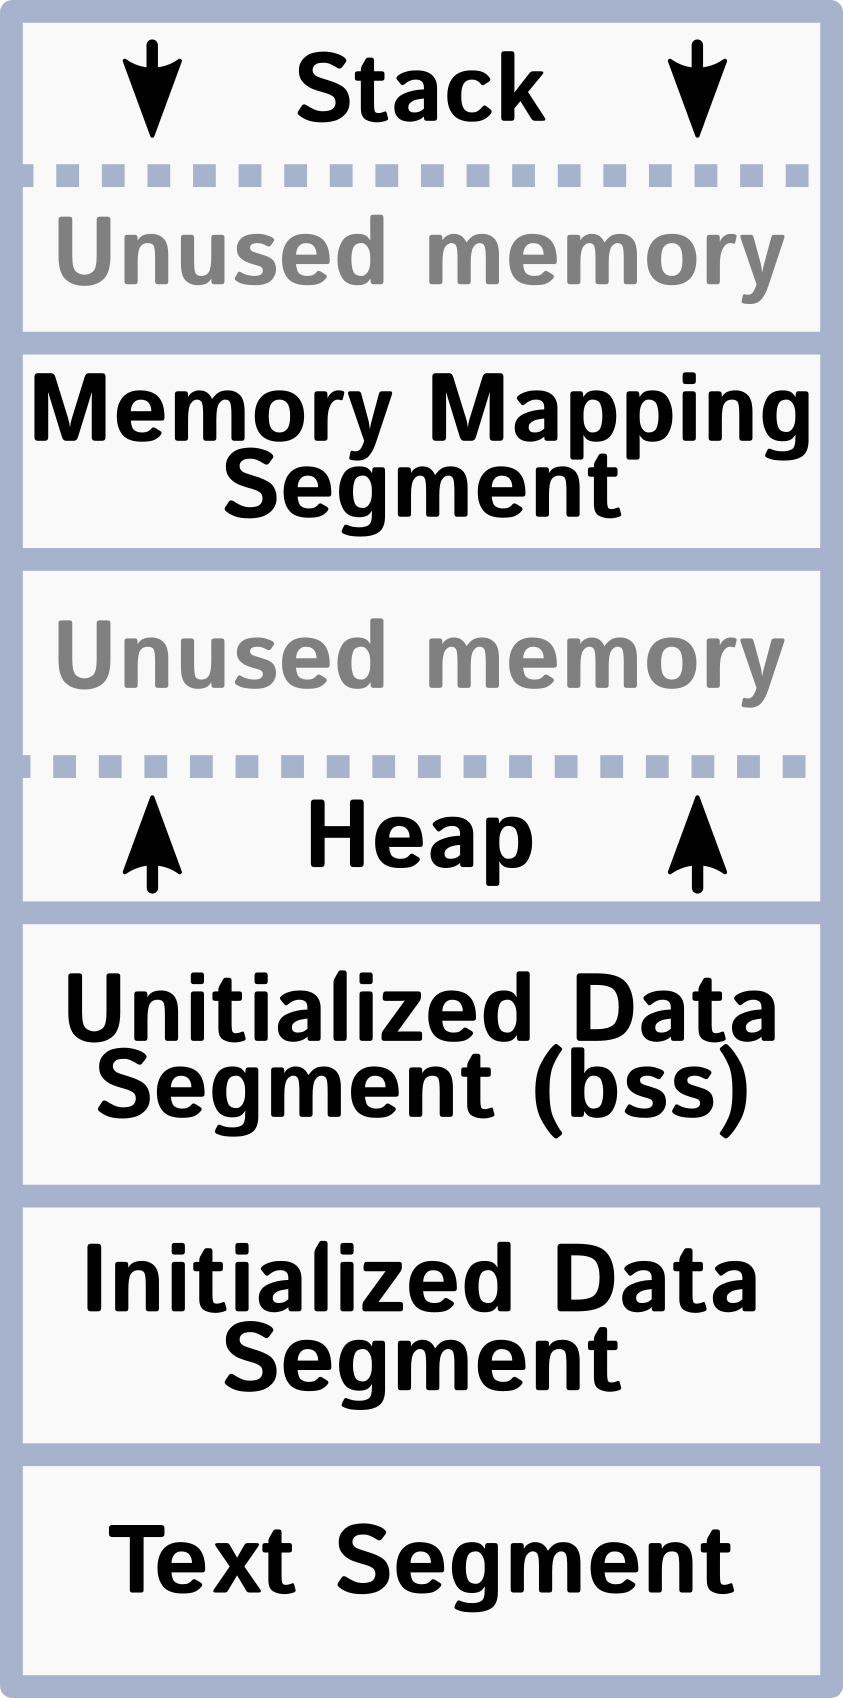
\includegraphics[width=.20\textwidth]{memory_segment} 
  \caption{Segmento de memória}
  \label{fig:memory_segment} 
\end{figure}

A Figura \ref{fig:memory_segment} ilustra seis segmentos de memória diferentes
representando o \emph{layout} de um processo após a criação dele por parte do
SO. O \boldAndIndex{segmento de texto} (\emph{Text Segment}) representa a região da
memória que mantém o código executável (compartilhável de somente
leitura). Já o \boldAndIndex{segmento de dados inicializáveis} (\emph{Initialized
Data Segment}) é responsável por manter variáveis estáticas, enquanto o
\boldAndIndex{segmento de dados não inicializados} (\emph{Uninitialized Data
Segment}) mantém variáveis estáticas não inicializadas.  Vale observar que o
segmento de dados não inicializável também é comumente conhecido como
\emph{Block Started by Symbol (BSS)} por causa de um antigo operador usado
pelos montadores \citep{gdb}. O \boldAndIndex{segmento de Mapeamento de Memória}
(\emph{Memory Mapping Segment}) é a região na qual o SO mapeia arquivos
diretamente na memória (e.g.; bibliotecas dinâmicas ou arquivos especificados
pelo programador). O \boldAndIndex{segmento da Stack} compreende aos dados usados
pelo programa durante a execução, como por exemplo, valores de parâmetros de
função, endereço de retorno e variáveis locais (dados temporários)
\citep{silberschatz}.  Por fim, o \boldAndIndex{segmento do Heap} mantém a memória
dinamicamente alocada durante a execução do programa; repare que o \emph{stack}
e o \emph{heap} estão em lados oposto da memória.

O primeiro passo realizado pelo SO quando ele lê o arquivo executável é olhar
para o \emph{header} e obter as informações sobre o tamanho do segmento de
texto e dados. Em seguida, com base nas informações obtidas do \emph{header}, o
SO cria um novo espaço de endereçamento (\emph{Address Space}) com tamanho de
memória suficiente para os segmento de texto e dados. Após alocar memória, o
próximo passo consiste em copiar toda a região de código e dados lidas do
arquivo binário para a memória recém alocada; complementarmente, é feita a
inicialização de todos os registradores e os devidos ajustes no \emph{stack
pointer}. O processo tem o seu \emph{Program Counter} (PC) ajustado para a
função \emph{main} do programa \citep{patterson}, por fim, o SO insere o novo
processo na fila do escalonador.

\begin{figure}[!h]
  \centering
  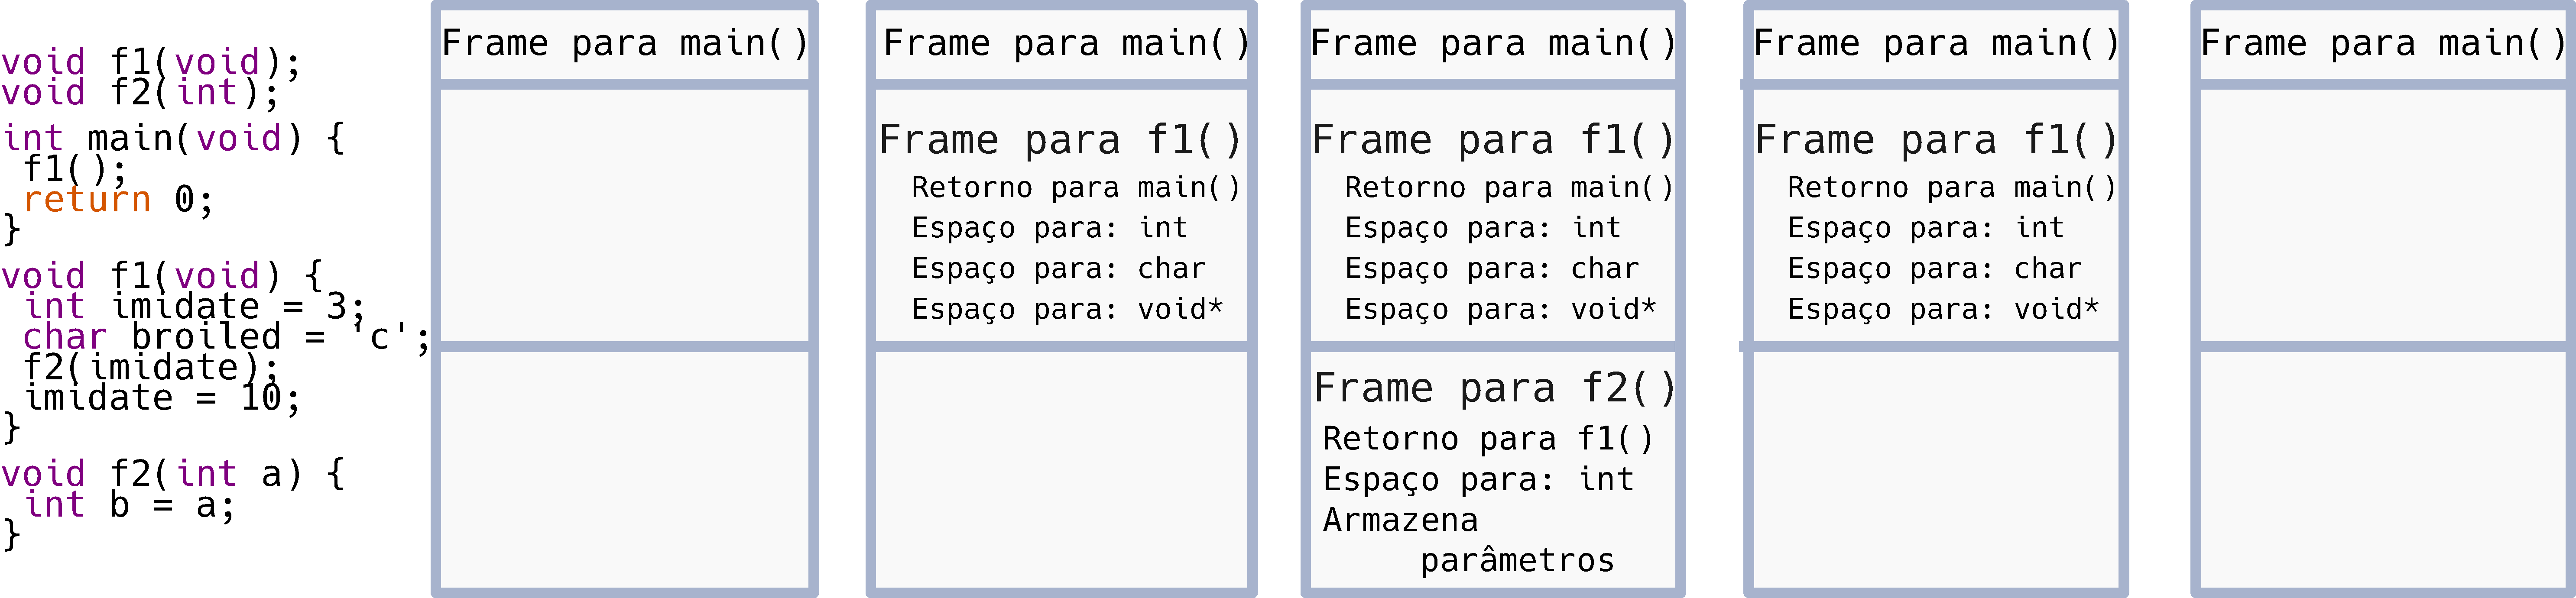
\includegraphics[width=\textwidth]{stack_frame}
  \caption{Stack frames, imagem baseada em \cite{patterson}}
  \label{fig:stack_frames} 
\end{figure}

% TODO: Fazer uma ponte melhor do PC com a execução

A \emph{stack} é organizada em uma coleção de \boldAndIndex{Stack Frames}. Toda vez
que uma função é chamada ela cria um novo \emph{frame} que mantém as variáveis
locais, argumentos e o ponto de retorno relacionado a função. Um processo pode
invocar um grande número de funções durante a sua execução, consequentemente,
cada função chamada recebe um \emph{stack frame}. A Figura
\ref{fig:stack_frames} ilustra a alocação e desalocação de um simples programa
\cite{gdb}. No começo, só existe um \emph{stack frame} associado no topo da
função \texttt{main}. Quando uma função local é chamada, o SO vai alocar um
novo \emph{stack frame} no topo do \emph{frame} da \texttt{main}, esse
procedimento permite que a execução do processo ocorra de forma consistente. No
fim da execução da função, ela retorna para o ponto na qual a função foi
invocada e o processo de preencher e esvaziar a \emph{stack} continua.

Todo os processos são descritos por meio de uma estrutura de dados chamado
\boldAndIndex{Process Control Block (PCB)} que é responsável por manter informações
sobre o status do processo, \emph{program counter} (PC), registradores da CPU,
informações sobre escalonamento, dados sobre contas de usuários, status de
operações de I/O e assim por diante \citep{silberschatz}. Uma dos principais
motivos para a PCB existir é o conceito de \textbf{troca de contexto} que é
responsável por colocar e tirar processos para executar em uma CPU. Por
exemplo, se o usuário tem vários processos rodando ao mesmo tempo, o SO tem que
mudar entre todos eles para que todos tenham a oportunidade de executar por um
intervalo de tempo. O SO realiza o processo de troca em duas etapas gerais: (1)
salva a PCB atual do processo e (2) carrega a PCB do outro processo. Em
poucas palavras, a troca de contexto tem que ser rápida uma vez que esta não
faz nenhum processamento considerado útil.

O conceito apresentado acima revela uma característica de isolamento associada
com a forma na qual os processos funcionam; normalmente, segurança e
estabilidade são positivamente afetadas pelo isolamento de processos. Por outro
lado, existem situações que exigem que os processos cooperem entre si e nesses
casos é possível notar algumas das desvantagens inerentes a estratégia de
processos atual. Para resolver parte desse problema, algumas bibliotecas ou
chamadas de sistemas são fornecidas como uma interface para coordenar a
interação entre processos executando concomitantemente, esses são conhecidos
pelo nome de \boldAndIndex{Interprocess Communication} (IPC). Por exemplo,
desenvolvedores podem utilizar IPC para compartilhar dados, melhorar o
desempenho das aplicações, modularizar ou por alguma questão de conveniência
da sua aplicação. O IPC tem três limitações principais: elevam o consumo de
memória, adicionam sobrecargas extras de comunicação e tem uma certa
complexidade para serem implementadas. Essas limitações são proibitivas em
aplicações com grande demanda computacional.

\begin{figure}[!h]
  \centering
  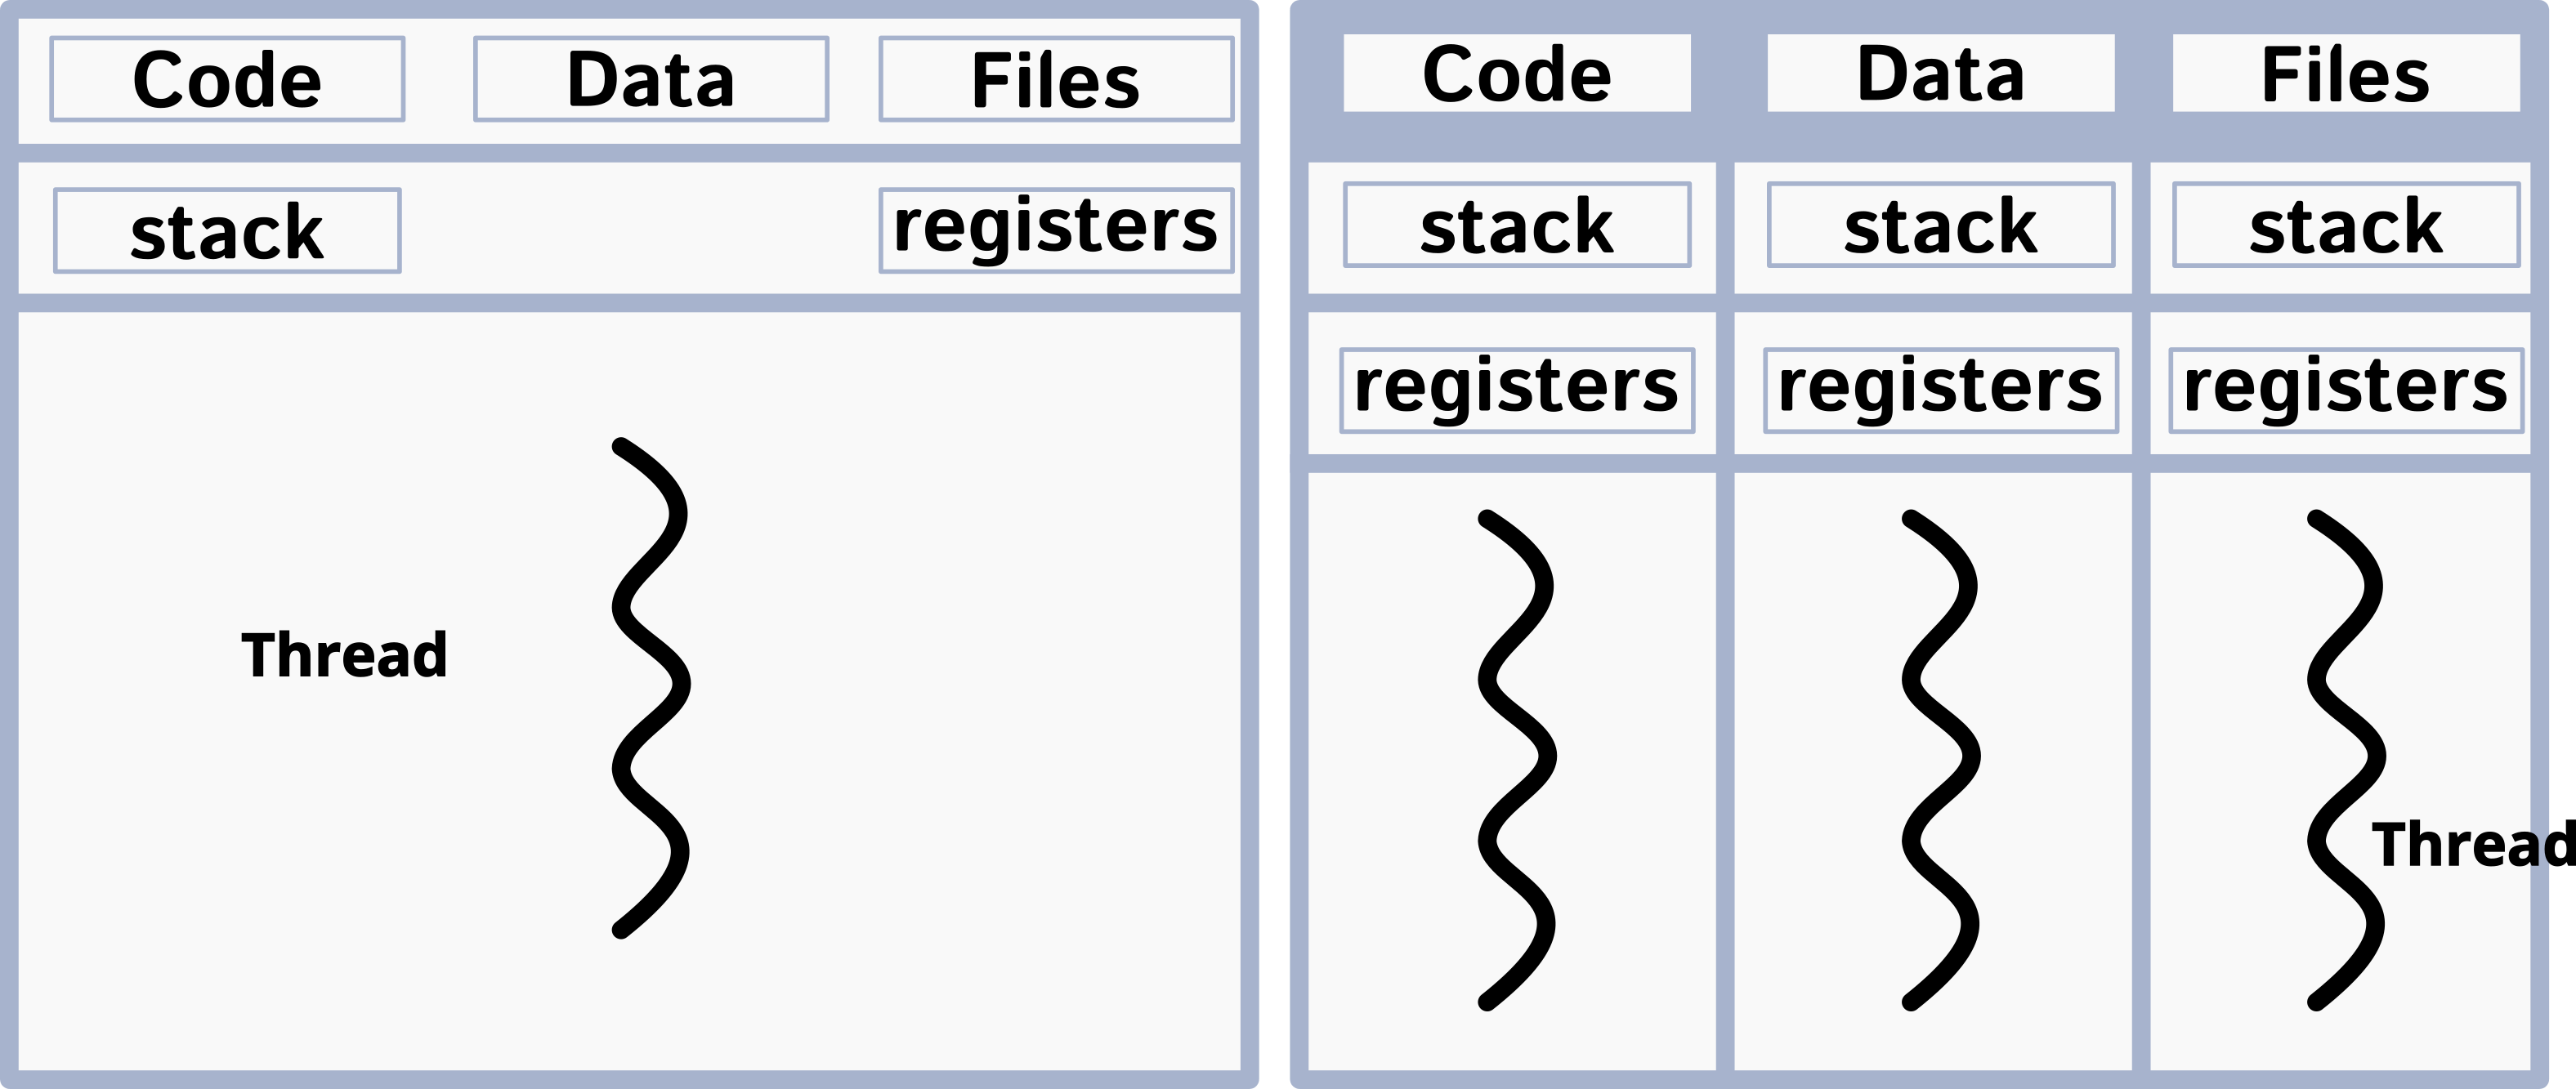
\includegraphics[width=.7\textwidth]{process_and_threads.png}
  \caption{Única thread e multi-thread, imagem baseada em \cite{silberschatz}}
  \label{fig:single_thread_multi_thread}
\end{figure}

Como é possível perceber, processos são abstrações poderosas com algumas
limitações, principalmente ao que se refere ao desempenho e complexidade. Além
disso, processos tem apenas um fluxo de execução (\textit{thread}) para
realizar todo o trabalho. Naturalmente os desenvolvedores buscam atingir mais
paralelismo ou concorrência por meio de IPC, contudo os programadores tem que
lidar com as sobrecargas extras impostas por essa estratégia. Por esse motivo,
buscou-se por muito tempo por formas de elevar o desempenho das aplicações por
meio de melhorias no grau de paralelismo. Como resultado direto de tal esforço
surgiu o conceito de um processo ter múltiplas \emph{threads} compartilhando
praticamente todos os elementos básicos com exceção da \emph{stack} e do PC. A
Figura \ref{fig:single_thread_multi_thread} mostra um processo com uma
\emph{thread} e outro com múltiplas \emph{threads}, note na figura o isolamento
da \emph{stack} e do PC.

\lstinputlisting[
                 language=C,
                 caption={Exemplo simple de threads},
                 label={lst:simplethreads}
                ]{code/simpleThread.c}

\begin{lstlisting}[frame=single,
                   language=bash,
                   caption={Saída do exemplo de threads},
                   label={lst:simpleThreadOutput}]
$ ./example 
Thread 1 
Thread 2
$ ./example
Thread 2 
Thread 1
\end{lstlisting}

O Código \ref{lst:simplethreads} ilustra o comportamento básico das
\emph{threads} por meio de uma biblioteca chamada de \emph{POSIX Thread Library
(Pthread)}. Veja no Código a criação de duas novas \emph{threads} que mostram
mensagens simples, note também que a implementação tem três \emph{threads}
diferentes: a \emph{thread} principal associada ao processo e outras duas
\emph{threads} diferentes criadas após a função \texttt{main()} iniciar a sua
execução. A função \texttt{thread\_kernel()} tem o código que é executado por
cada nova \emph{thread} criada na função principal. Note que
\texttt{thread\_kernel} recebe um ponteiro genérico, converte esse para um tipo
\texttt{char} e mostra o valor no final.

A função \texttt{main()} declara duas variáveis do tipo \texttt{pthread\_t}, que
são responsáveis por manter as informações referêntes as \emph{threads}.
Adicionalmente, são declaradas duas \emph{strings} de mensagens para serem
mostradas posteriormente dentro das \emph{threads} criadas. Quando o programa
chega na função \texttt{pthread\_create()}, a biblioteca solicita ao SO a
criação de uma nova \emph{thread} que executa a função \texttt{thread\_kernel}
em paralelo. A função \texttt{pthread\_create()} é chamada novamente e cria a segunda
\emph{thread} de execução baseada na função \texttt{thread\_kernel}, contudo,
com outra mensagem associada com ela. O código termina com a função
\texttt{pthread\_join()}, que mantém a \emph{thread} princípal até que as duas
\emph{threads} terminem a sua execução. A saída ilustrada em
\ref{lst:simpleThreadOutput} mostra as duas execuções que aconteceram em
paralelo, isso pode ser percebido pela sequência não determinística da saída. A
diferença na sequência é explicada pela variação imposta pelo escalonador.

\begin{figure}[!h]
  \centering
  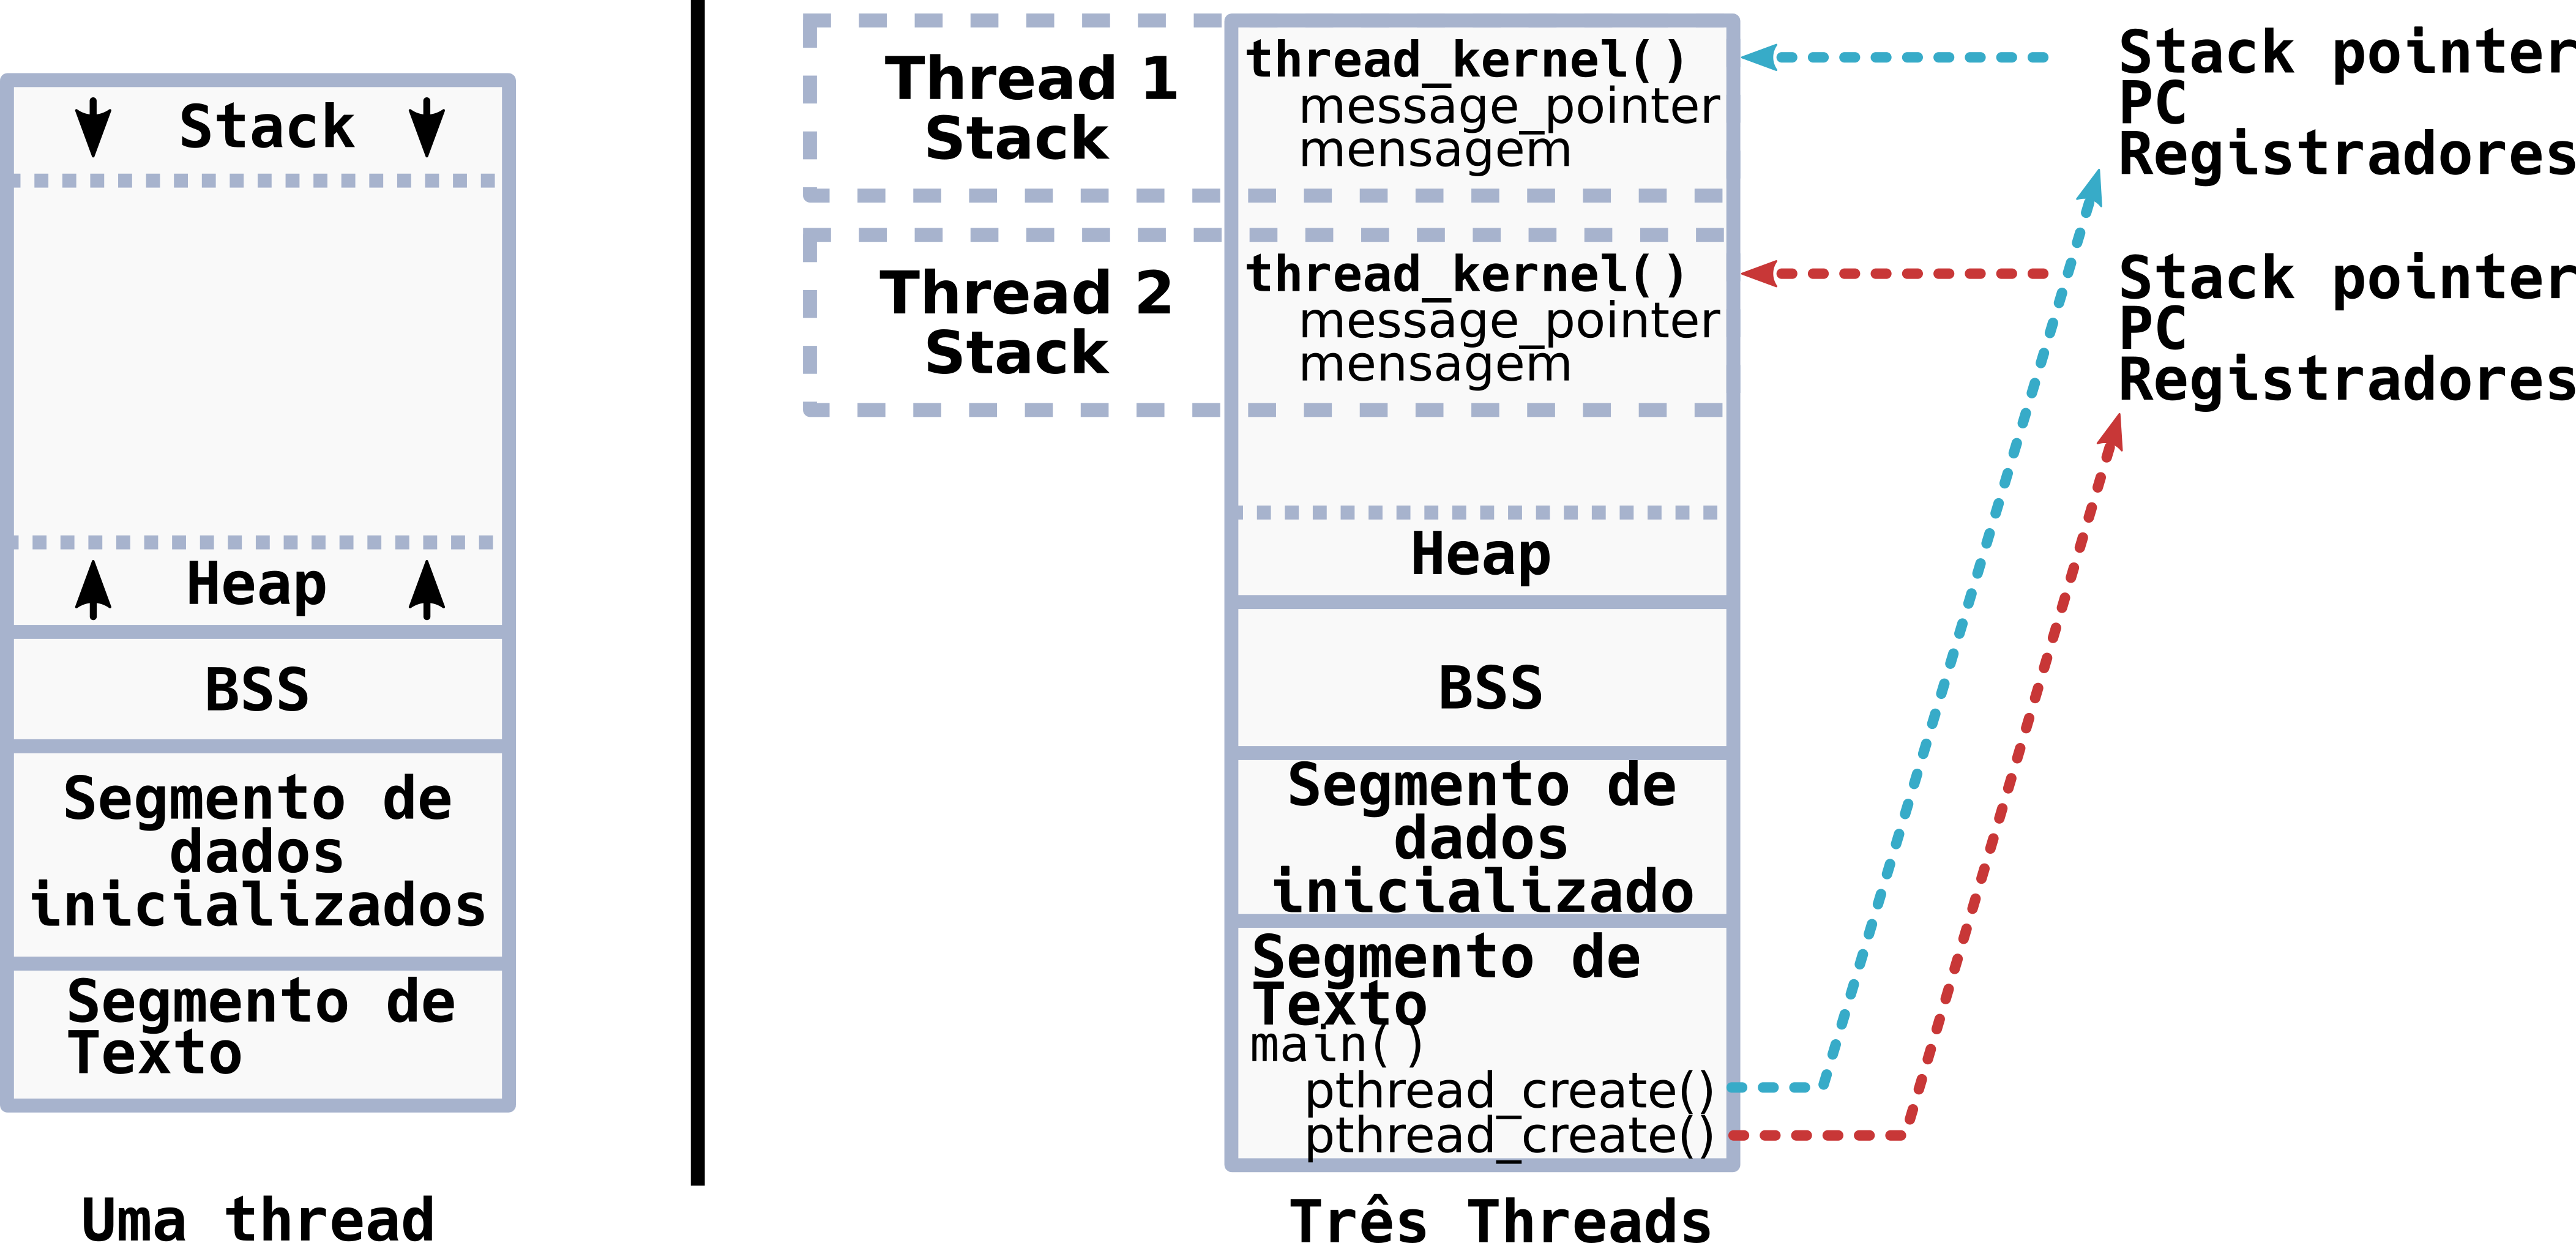
\includegraphics[width=.60\textwidth]{theads_and_stack} 
  \caption{Stack com duas threads}
  \label{fig:stack_threads} 
\end{figure}

Para a melhor compreensão de como o SO trata o Código \ref{lst:simplethreads}
durante a execução, veja a Figura \ref{fig:stack_threads} ilustrando o que
acontece da perspectiva do processo. Como esperado, o segmento de texto e dados
é compartilhados entre as \emph{threads}. A principal mudança pode ser
observada no segmento da \emph{stack}, toda vez que uma nova \emph{thread} é
criada um novo segmento de \emph{stack} é gerado; a independência entre
\emph{threads} é assegurada por multiplas \emph{stacks} isoladas. Toda vez que
a \emph{thread} é mudada, o \emph{stack pointer} e os registradores são
atualizados.

\section{Gerenciamento da Memória relacionada aos processos}

% TODO: Merge com a próxima seção
Fazer com que a memória do sistema esteja disponível e utilizável para uma
aplicação representa uma das principais responsabilidade de um SO. A maioria
dos SOs oferece a ilusão de que toda a memória está acessível para o processo,
isso é possível devido ao desacoplamento da memória física de como um processo
a vê. Processos só veem o \emph{Virtual Address Space (VAS)}, por sua vez, esse
é mapeado por um SO (com auxílio de hardware) para uma memória física o que
garante um bom isolamento entre processos. Para manipular VASes e oferecer um
recurso útil para a aplicação do usuário, os SOs tem que adotar um modelo de
memória especifica; atualmente, a maioria dos SOs de produção e hardware
suportam amplamente o modelo de gerenciamento de páginas.  Esse modelo separa a
VAS e o espaço de endereçamento físico para cada processo em um conjunto de
páginas, essas tem um pequeno intervalo contíguo de endereços, tamanho fixado,
endereço de início e permissões. O modelo de paginação tem algumas vantagens:
controle das permissões no nível da página, mecanismos de compartilhamento,
rápida verificação de proteção, notificações acuradas sobre violações e a
possibilidade de mapear memória em disco.

\subsection{Endereços lógicos, físicos e Paginação}

% TODO: 
Nessa seção, não temos a intenção de discutir profundamente os mecanismos presentes 

Imagine um programa escrito em C, em algum momento do código esse faz uma
alocação de memória e em um outro momento essa região é lida ou escrita. Esse
programa de alto nível é traduzido para um conjunto de instruções de baixo
nível na qual a CPU consegue manipular, o arquivo contendo essas informações é
comumente chamada de binário.  Posteriormente esse binário é carregado pelo SO
e o programa começa a sua execução. Durante a realização das tarefas da
aplicação, naturalmente ocorrem acessos aos endereços de memória. Da relação
entre o código de alto nível, o binário e o acesso a memória, surgem algumas
questões, dentre elas: como o programa consegue acessar o endereço sem conhecer
as características da máquina? Como os programas evitam os acessos aos mesmos
endereços?

A resposta para as perguntas acima nascem de três conceitos: \textit{address
binding} em tempo de execução, espaço de endereçamento e paginação. O processo
de "construção" do endereço nasce durante a compilação do código fonte, nesse
momento o compilador consegue identificar diversos tipos de acesso a memória
(não entraremos em detalhes, por fugir do escopo desse trabalho) e este faz uma
marcação em certos endereços que indicam que o mesmo deve ser definido em tempo
de execução. Com base nessa "marcação" os SO e o hardware ganham um mecanismo
para definir o endereço em tempo de execução.

Como dito anteriormente, o binário contém certas informações necessárias para a
criação do processo e também para a definição de acesso de um endereço. Quando
o software começa a sua execução, significa que a CPU está executando as
instruções descritas no binário, dentre elas as tentativas de acesso a certos
endereços na memória.

Todo endereço gerado pela CPU recebe o nome de \boldAndIndex{endereço virtual} ou
\textbf{endereço lógico}\index{Endereço lógico}, por sua vez, o conjunto desses
endereços recebe o nome de \boldAndIndex{espaço de endereçamento virtual (Virtual
Address Space)} ou simplesmente VAS. De forma simplificada, podemos dizer que
esses endereços gerados pela CPU não são válidos da perspectiva da memória,
i.e., são apenas endereços usados pela aplicação mas que não correspondem ao
endereço real da memória física. Os endereços reais da memória são chamados de
\boldAndIndex{endereços físicos} e o conjunto de todos os endereços da memória são
chamados de \boldAndIndex{espaço de endereçamento físico}. Agora você deve está se
perguntando: qual a relação entre esses dois tipos de endereços? Como eles
ajudam a resolver os problemas citados no começo? Eis que surge um terceiro
elemento entre esses conceitos, o \textit{Memory-Management Unit
(MMU)}\index{MMU}. Veja a Figura \ref{fig:mmu} ilustrando a posição "física"
desse hardware:

\begin{figure}[!h]
  \centering
  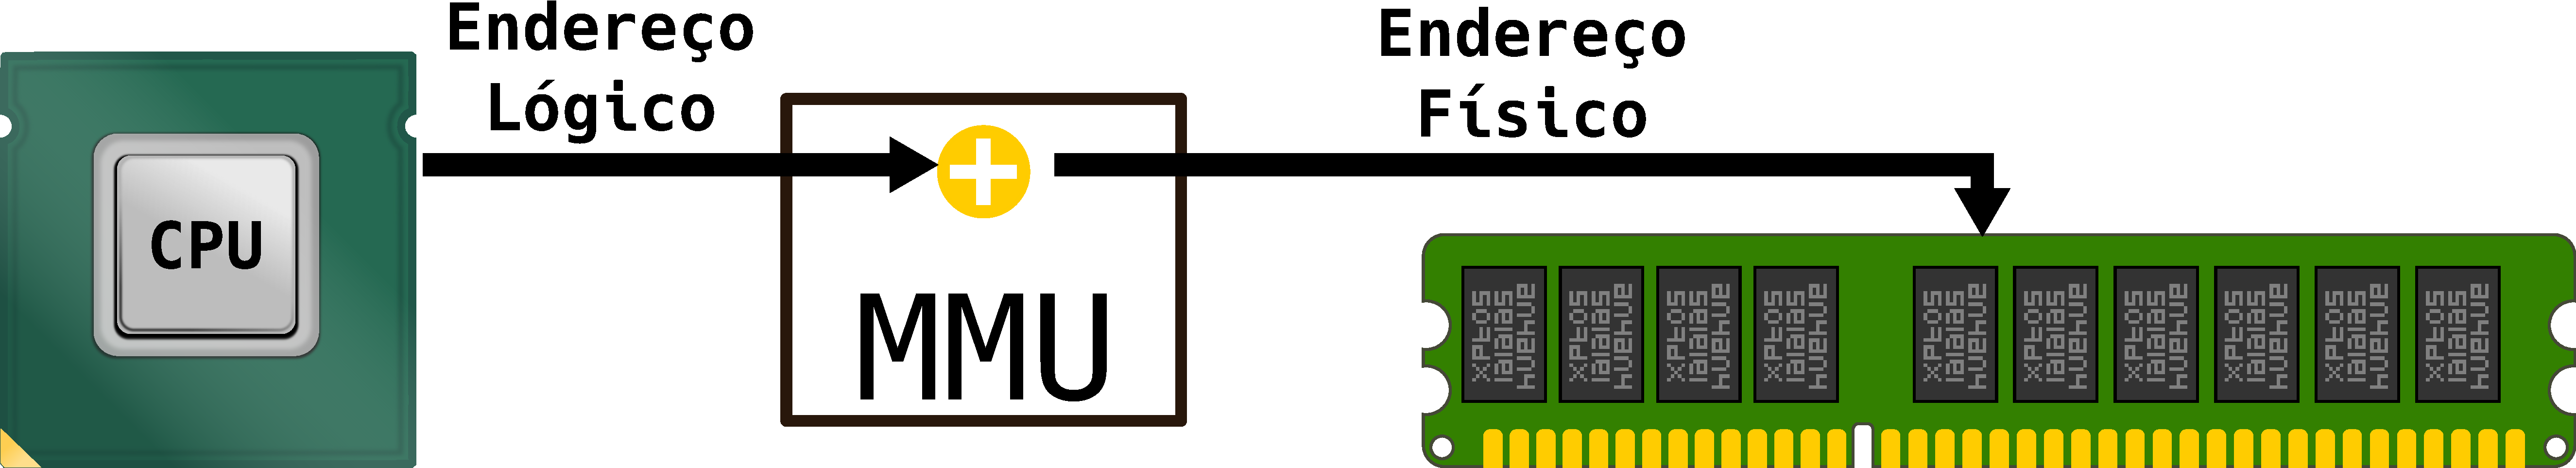
\includegraphics[width=\textwidth]{mmu} 
  \caption{Representação didática da MMU}
  \label{fig:mmu}
\end{figure}

A MMU é um hardware usado para fazer o mapeamento do endereço virtual para o
endereço físico em tempo de execução. A Figura \ref{fig:mmu} mostra a CPU
gerando um endereço, que por sua vez é entregue a MMU. A MMU converte o
endereço virtual em um endereço físico e procede com o acesso a memória. Dado a
visão geral do que acontece do endereço virtual para o endereço físico com o
intermédio da CPU, podemos olhar com mais detalhes o funcionamento do
mapeamento e introduzir o conceito de paginação.

Antes de nos aprofundarmos na paginação, vale a pena fazer uma última reflexão
sobre os endereços físicos e virtuais. Começando com os endereços virtuais,
repare que esses precisam ter algum intervalo definido e que seja finito, qual
seria? Esse intervalo começa em 0 e vai até um valor máximo definido em um
conjunto de bits chamado de \textit{virtual bits}. Durante muito tempo, o total
de bits era de 32 o que dava um espaço de endereçamento de 4 Gb; hoje em dia é
relativamente simples encontrar CPUs com 48 bits o que gera uma VAS de 256 TiB.
Na prática, isso significa que um software executando em um SO moderno tem a
ilusão de que pode acessar todos os endereços fornecidos pela VAS. Por
enquanto, sabemos que isso não é verdade, pois dificilmente conseguimos
fornecer tanta memória. Por esse motivo e como ilustrado na Figura
\ref{fig:vas_pas}, notamos que o endereço virtual é várias vezes maior do que o
endereço físico. Para piorar, a memória física deve ser compartilhada entre
vários processos em execução no SO.

\begin{figure}[!h]
  \centering
  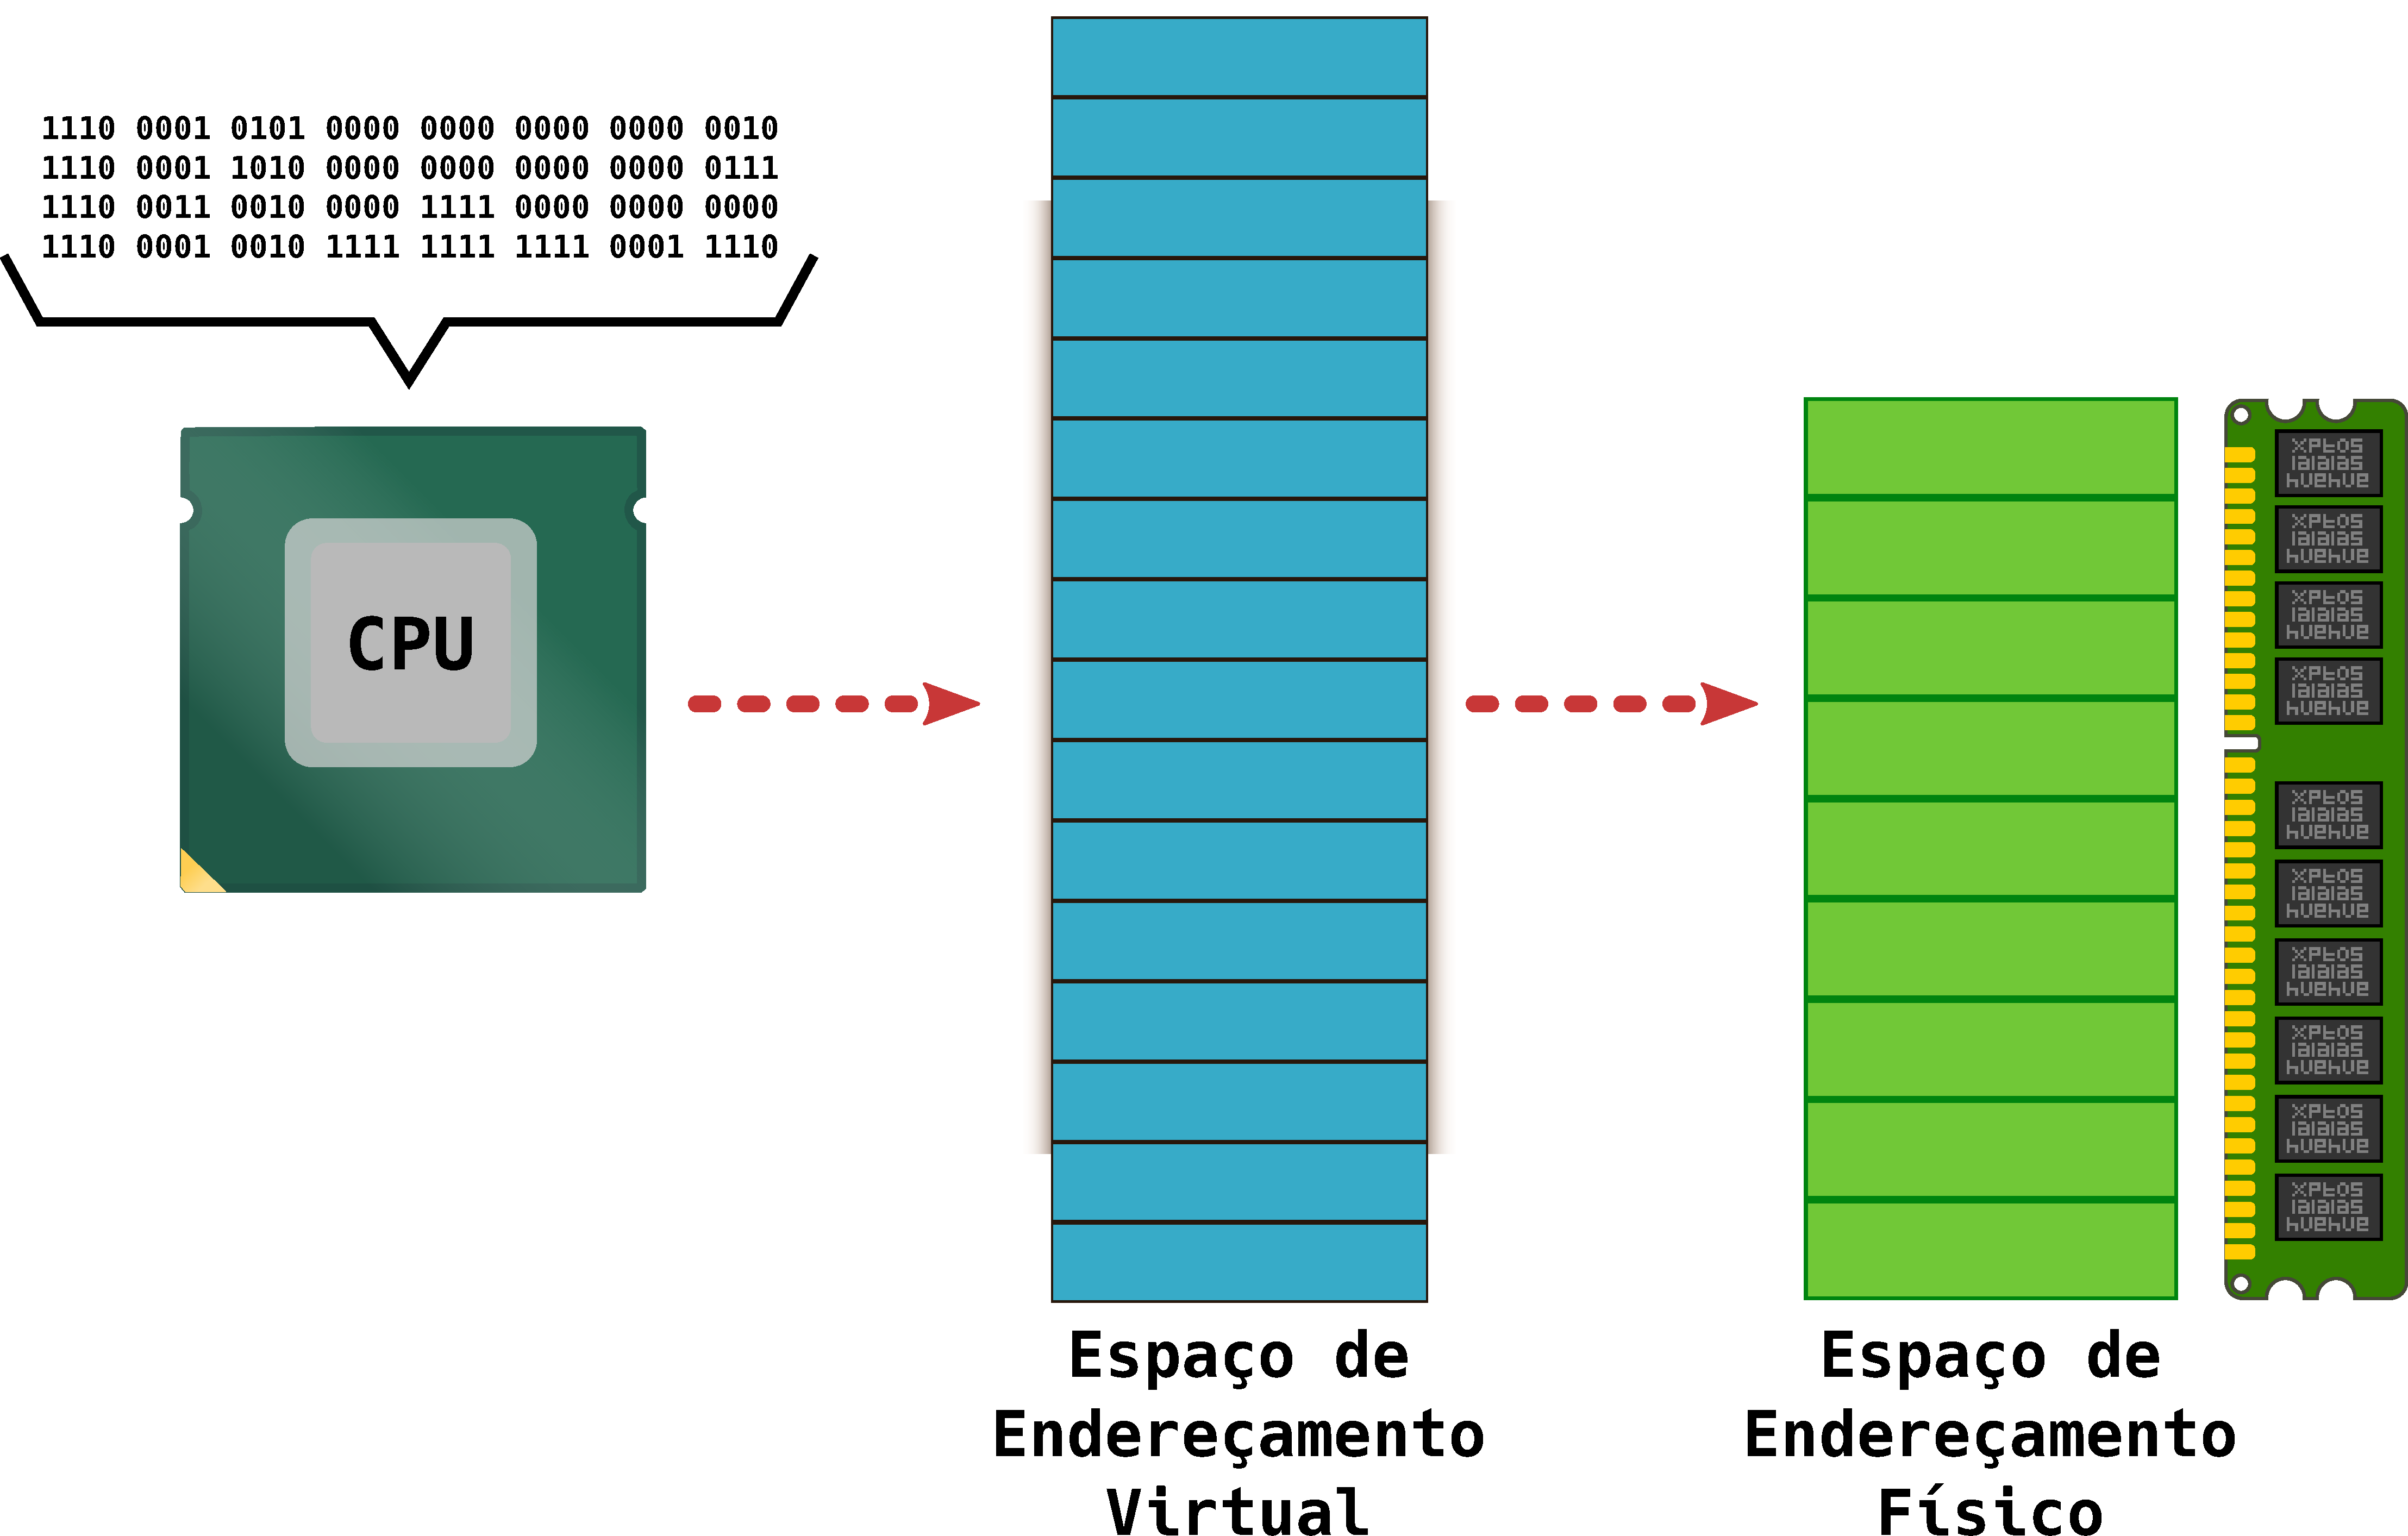
\includegraphics[width=\textwidth]{virtual_vs_fisico} 
  \caption{Espaço de endereçamento virtual vs. físico}
  \label{fig:vas_pas}
\end{figure}

O modelo de paginação é um esquema que surge com o objetivo de permitir que os
endereços físicos do processo possam ser dispostos na memória de forma
não-contínua. A implicação direta desse modelo é a de que um processo não
precisa estar totalmente na memória e que esse conceito se sustenta para "n"
processos. Contudo, para que tal modelo possa ser implementado, é preciso
dividir o espaço de endereçamento virtual e físico em \boldAndIndex{páginas} e
\boldAndIndex{frames} respectivamente. Uma vez que ambos os espaços de endereçamentos
são subdivididos, é necessário ter um mecanismo para saber o que está presente
ou não na memória. Para ter uma visão de como todo o modelo de paginação
funciona, veja a Figura \ref{fig:paginacao}.

\begin{figure}[!h]
  \centering
  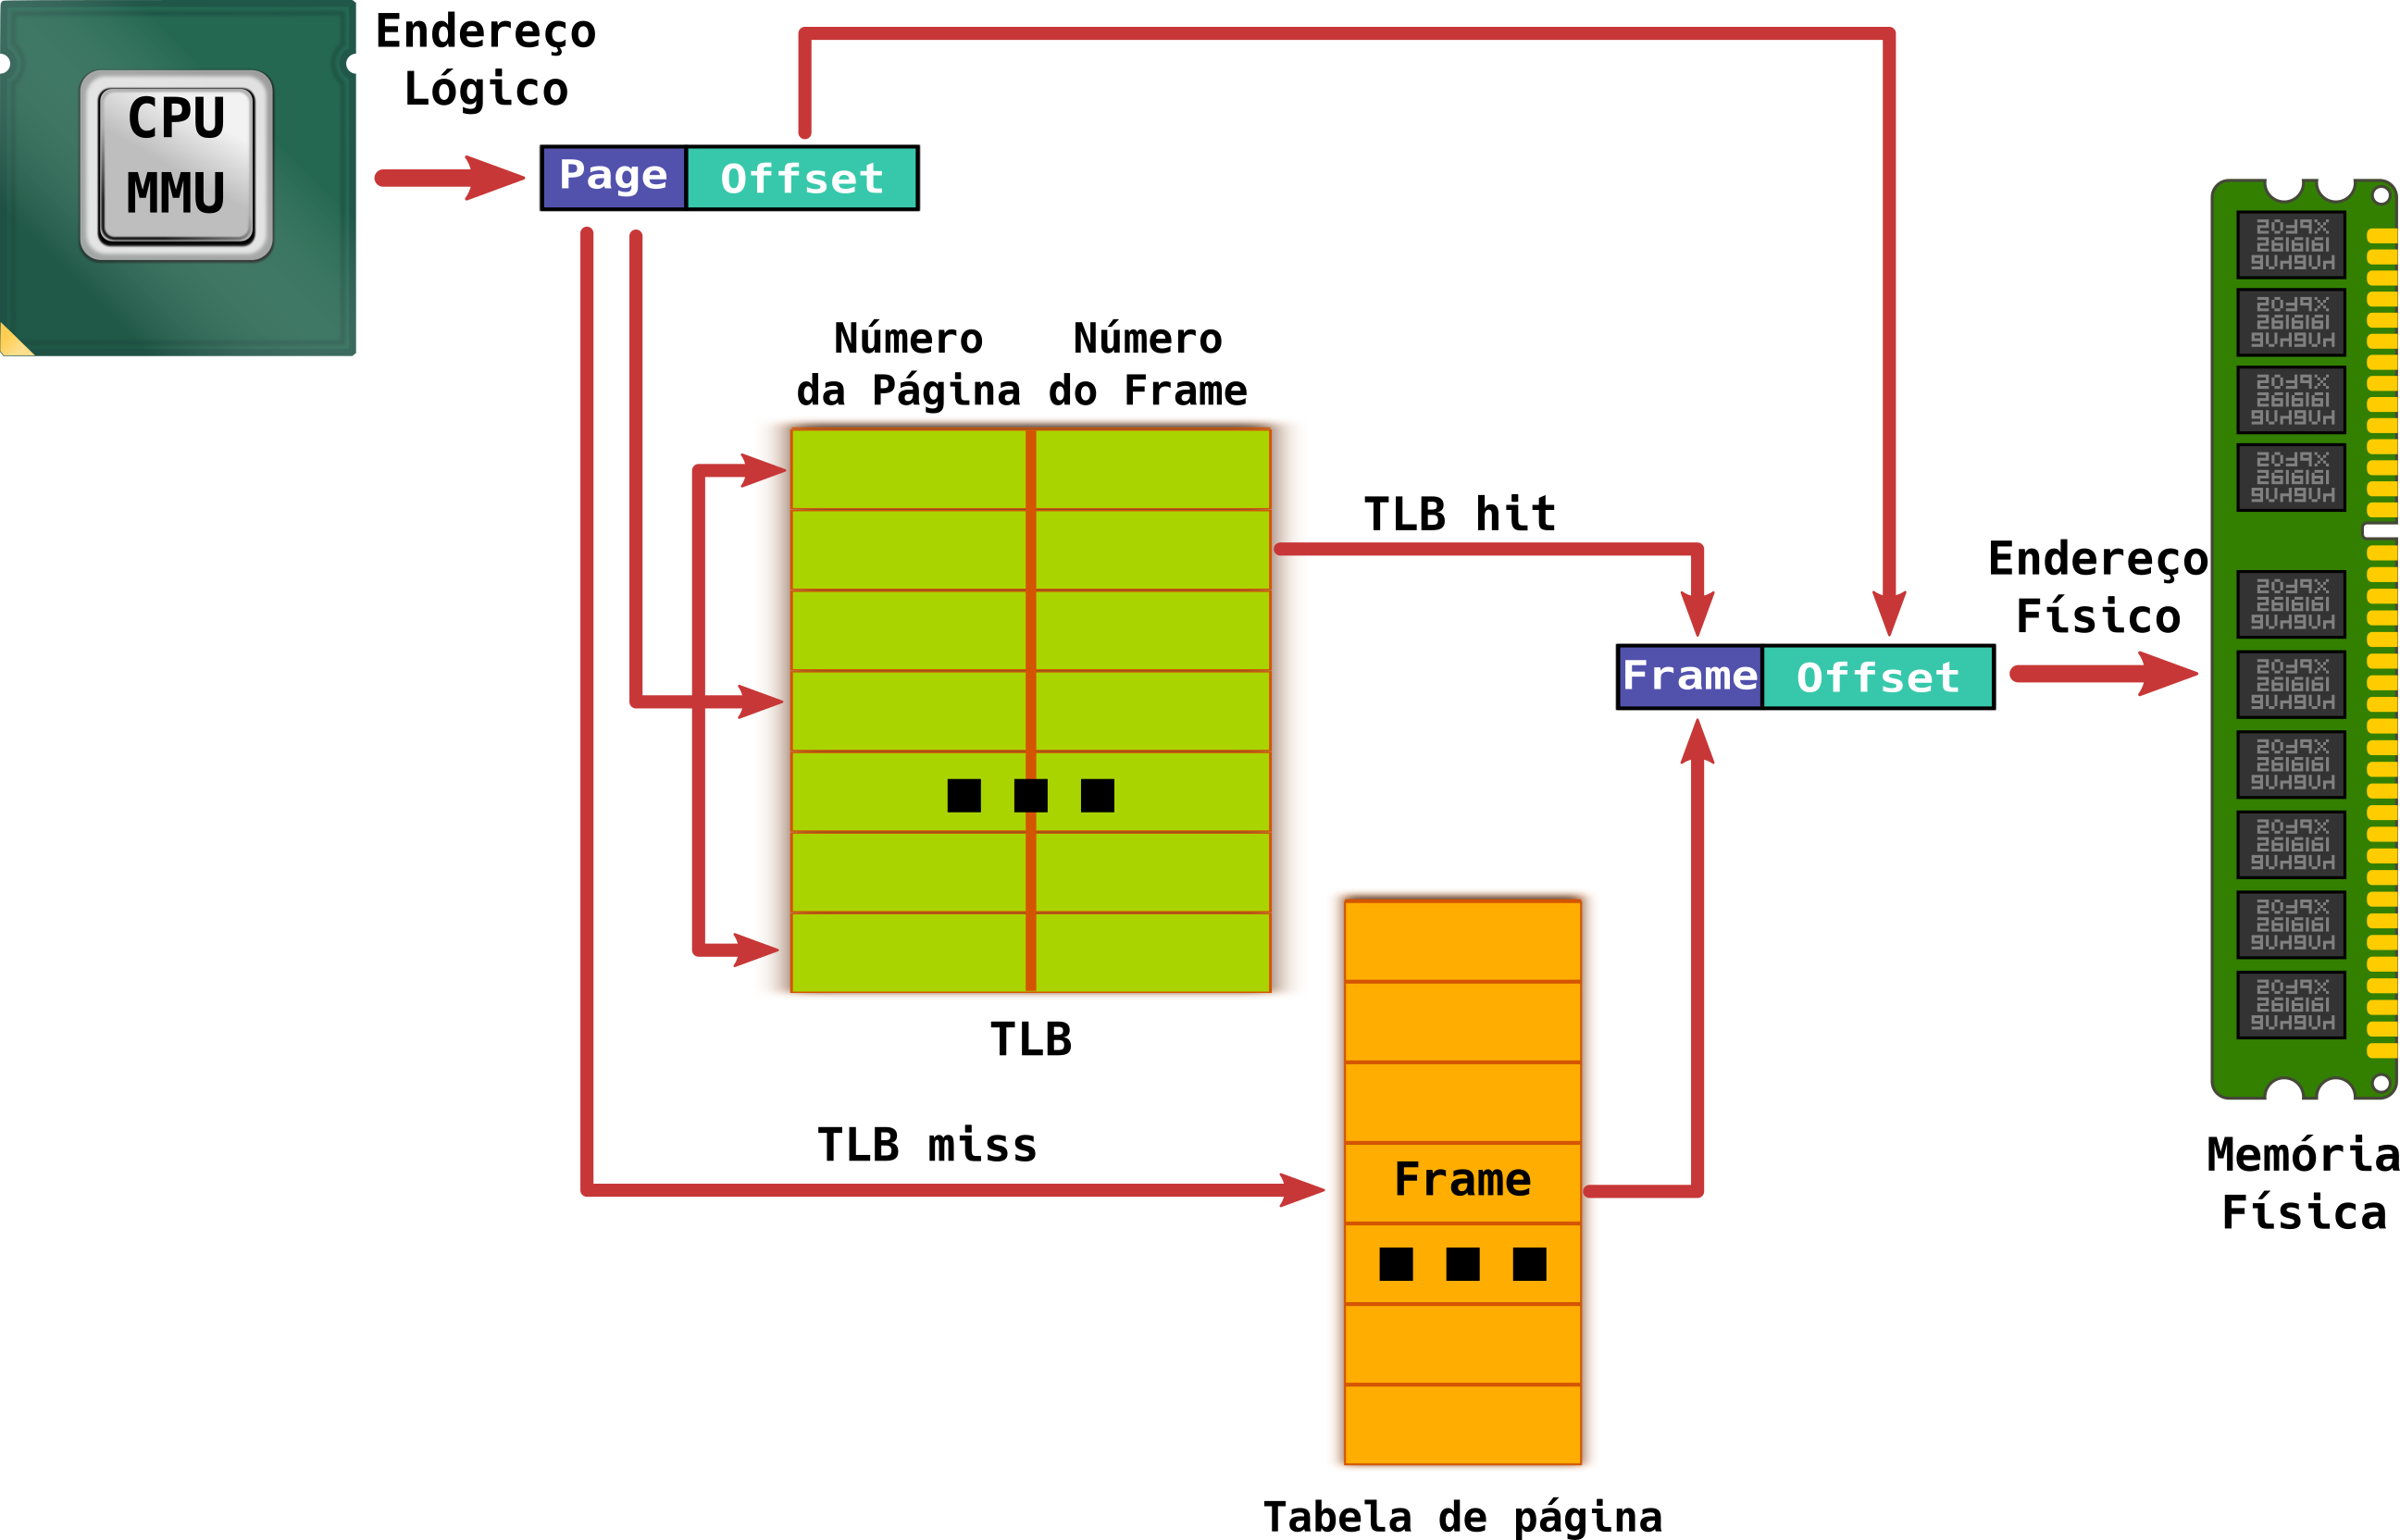
\includegraphics[width=0.8\textwidth]{paginacao} 
  \caption{Modelo de paginação}
  \label{fig:paginacao}
\end{figure}

Na Figura \ref{fig:paginacao} observamos que a CPU gera um endereço lógico, por
sua vez esse endereço é subdividido em duas partes: um \textit{page} e um
\textit{offset}. O page comporta-se como um index corresponde a uma entrada em
uma estrutura de dados chamada de \boldAndIndex{Tabela de Paginação}, essa tabela faz
parte da abstração de processos e tem uma entrada especificada na PCB, ou seja,
todo processo tem tal tabela associada a si. Cada entrada na tabela corresponde
ao endereço de início de um frame na memória que está associado ao processo.
Para ilustrar melhor esse conceito, imagine um programa que aloca espaço na
memória, na prática o SO cria uma nova entrada na tabela e retorna o endereço
virtual para a aplicação.  Depois que o valor referente ao index é recuperado a
MMU soma o \textit{offset} da segunda parte do endereço virtual e finalmente o
acesso a memória física ocorre.

\begin{figure}[!h]
  \centering
  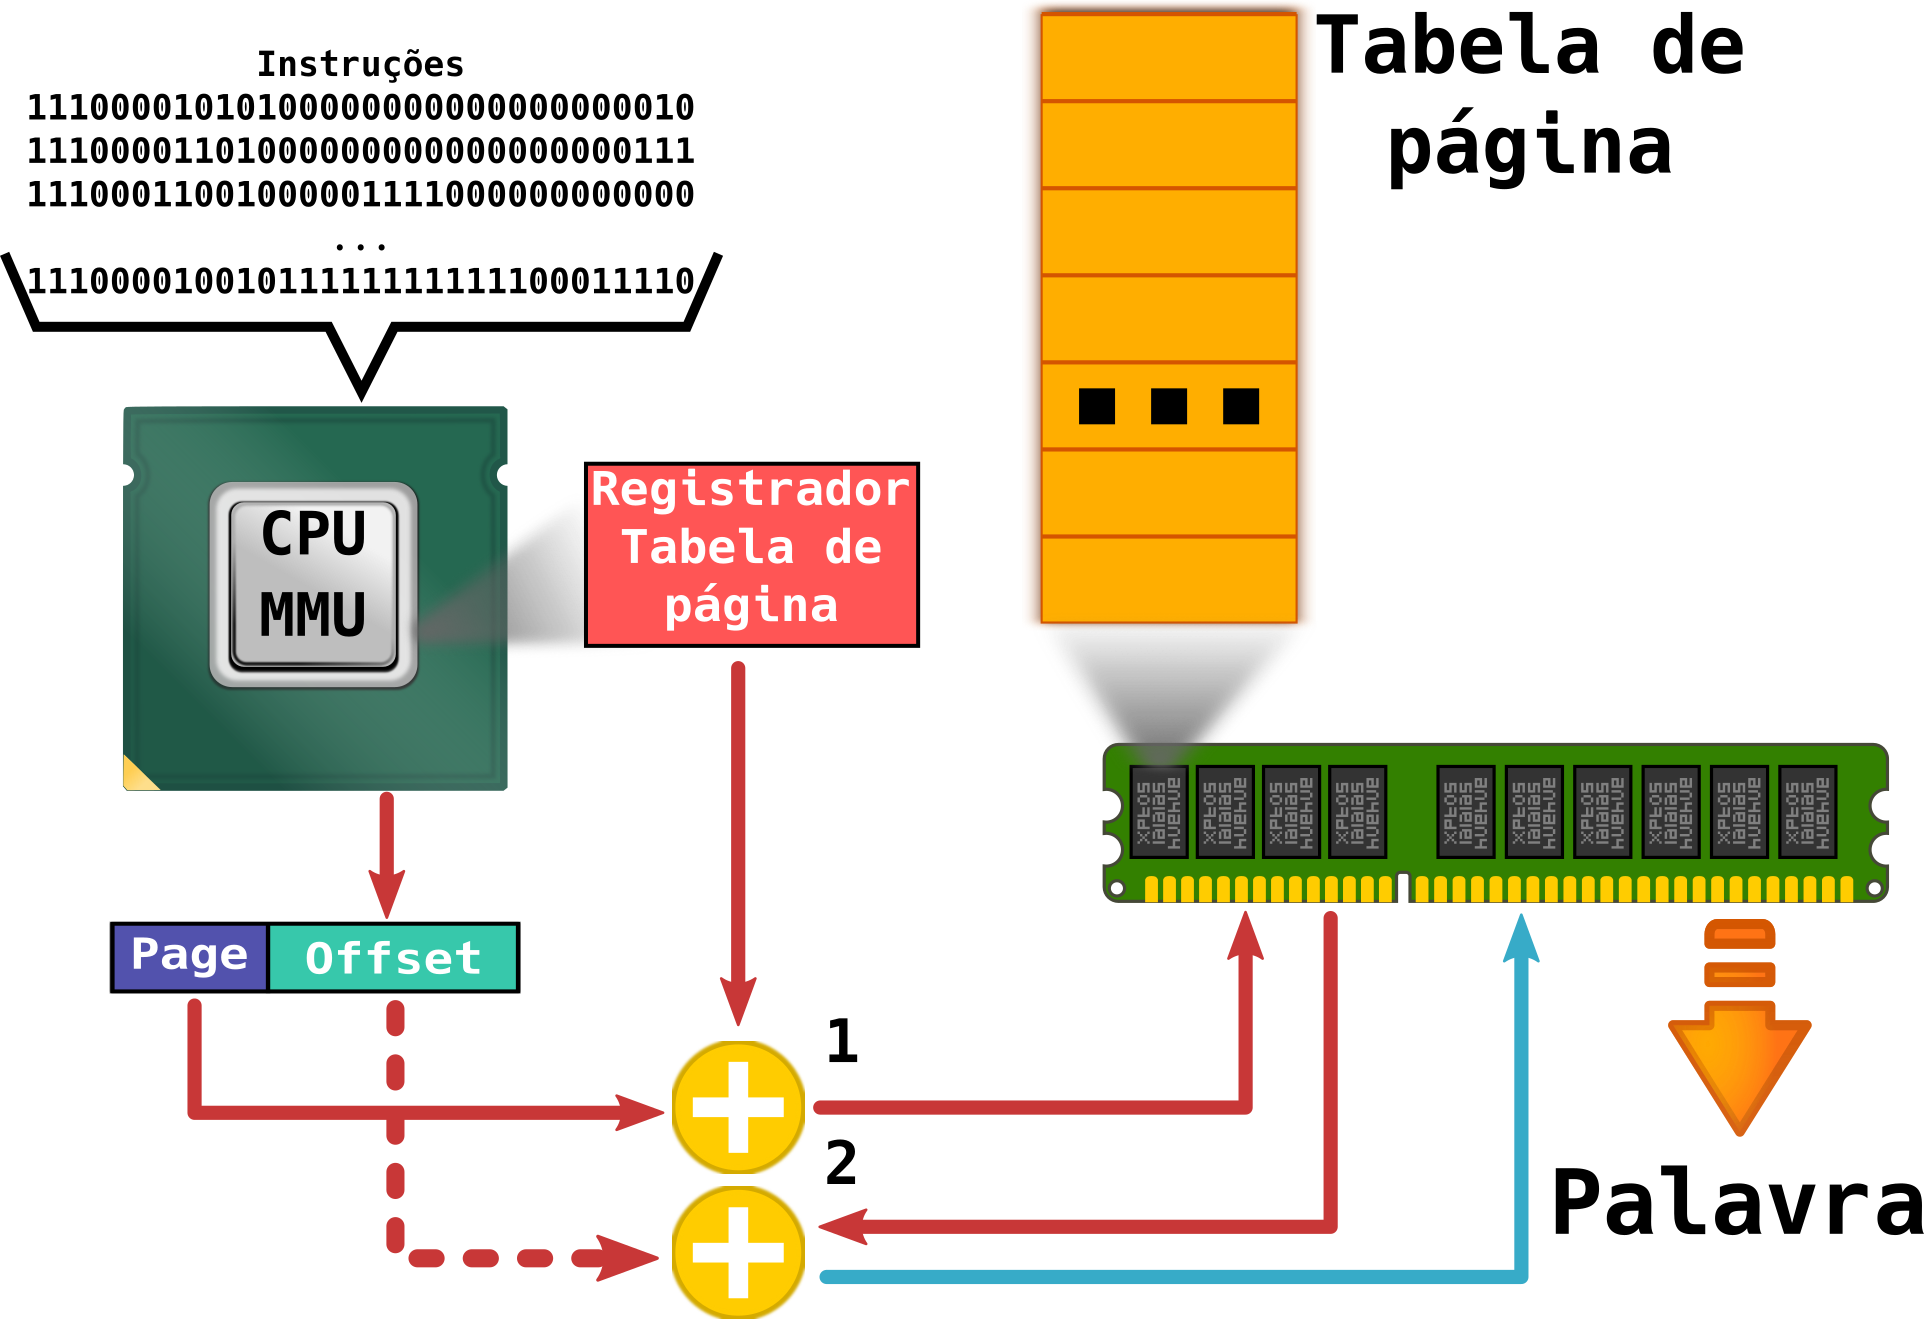
\includegraphics[width=0.8\textwidth]{paginacao_passos} 
  \caption{Passos do acesso a memória com paginação}
  \label{fig:passos_paginacao}
\end{figure}

A Figura \ref{fig:passos_paginacao} exemplifica o processo descrito
anteriormente. Repare que são necessários vários acessos a memória para
construir o endereço final e finalmente conseguir acessar a palavra de dados,
claramente isso não é eficiente. Nesse sentido, existe um mecanismo que busca
reduzir esses acessos por meio de uma tabela chamada de \boldAndIndex{Translation
look-aside Buffer (TLB)}. Essa tabela salva o último acesso (coluna e valor)
feito a tabela de páginas evitando que a memória seja consultada inúmeras
vezes. Tal mecanismo é ilustrado na Figura \ref{fig:paginacao}, note que a
busca na TLB e na tabela de página ocorre em paralelo, se a TLB tiver um acerto
a procura na da memória; do contrário, \textit{TLB Miss}, a busca na memória já
se inciou.

Por fim, é importante destacar que os mecanismos descritos nessa seção trazem
inúmeros benefícios diretos e indiretos. Talvez as vantagens mais direta seja a
possibilidade de ter o processo na memória de forma não contígua e assim
conseguir controlar o que deve ou não estar presente na memória. Indiretamente,
esses mecanismos isolam cada processo de acordo com a VAS uma vez que todo
processo tem a ilusão de que tem total controle da memória. Além disso, o
mecanismo de paginação facilita a operação de realizar o compartilhamento de
dados entre os processos; o SO orquestra um conjunto de páginas com a mesma
visibilidade (indicada pelo programa no espaço de usuário) para ser
compartilhado entre processos.

\subsection{Modelo de Segmentação}

Além do mecanismo de gerenciamento de memória fornecido pela paginação, também
existe uma alternativa chamada de segmentação. Esse modelo divide o memória
referente ao programa de acordo com as suas seções, empiricamente esse modelo
comporta-se dividindo programa em um conjunto de segmentos, por exemplo, uma
área para o \textit{text}, outra para os dados, \textit{stack}, etc. Os
tamanhos de cada segmento podem ser variáveis, o que leva a uma visão
bidimensional da memória uma vez que os endereços passam a ser construído como
uma tupla: \\

\texttt{<número do segmento, offset>}~\citep{silberschatz}.

O modelo de segmentos oferece uma visão bidimensional, mas a memória continua
sendo linear, por isso é necessário converter os endereços.
A Figura G mostra como a segmentação funciona com o suporte de hardware, repare
que o endereço gerado pela CPU é dividido em duas partes. A primeira parte do
endereço corresponde ao número do segmento salvo na tabela de segmentos, por
sua vez, o valor associado ao index é um endereço presente na memória física.
Como ilustrado na figura, a tabela de segmentos tem dois valores: limite e
base. O limite é o tamanho máximo do segmento e é usado para verificar se o
offset passado é valido. O segundo valor, base, é o começo do segmento na
memória física. Se tudo estiver certo, o endereço final é acessado utilizando a
soma do valor base com o offset.

\begin{figure}[!h]
  \centering
  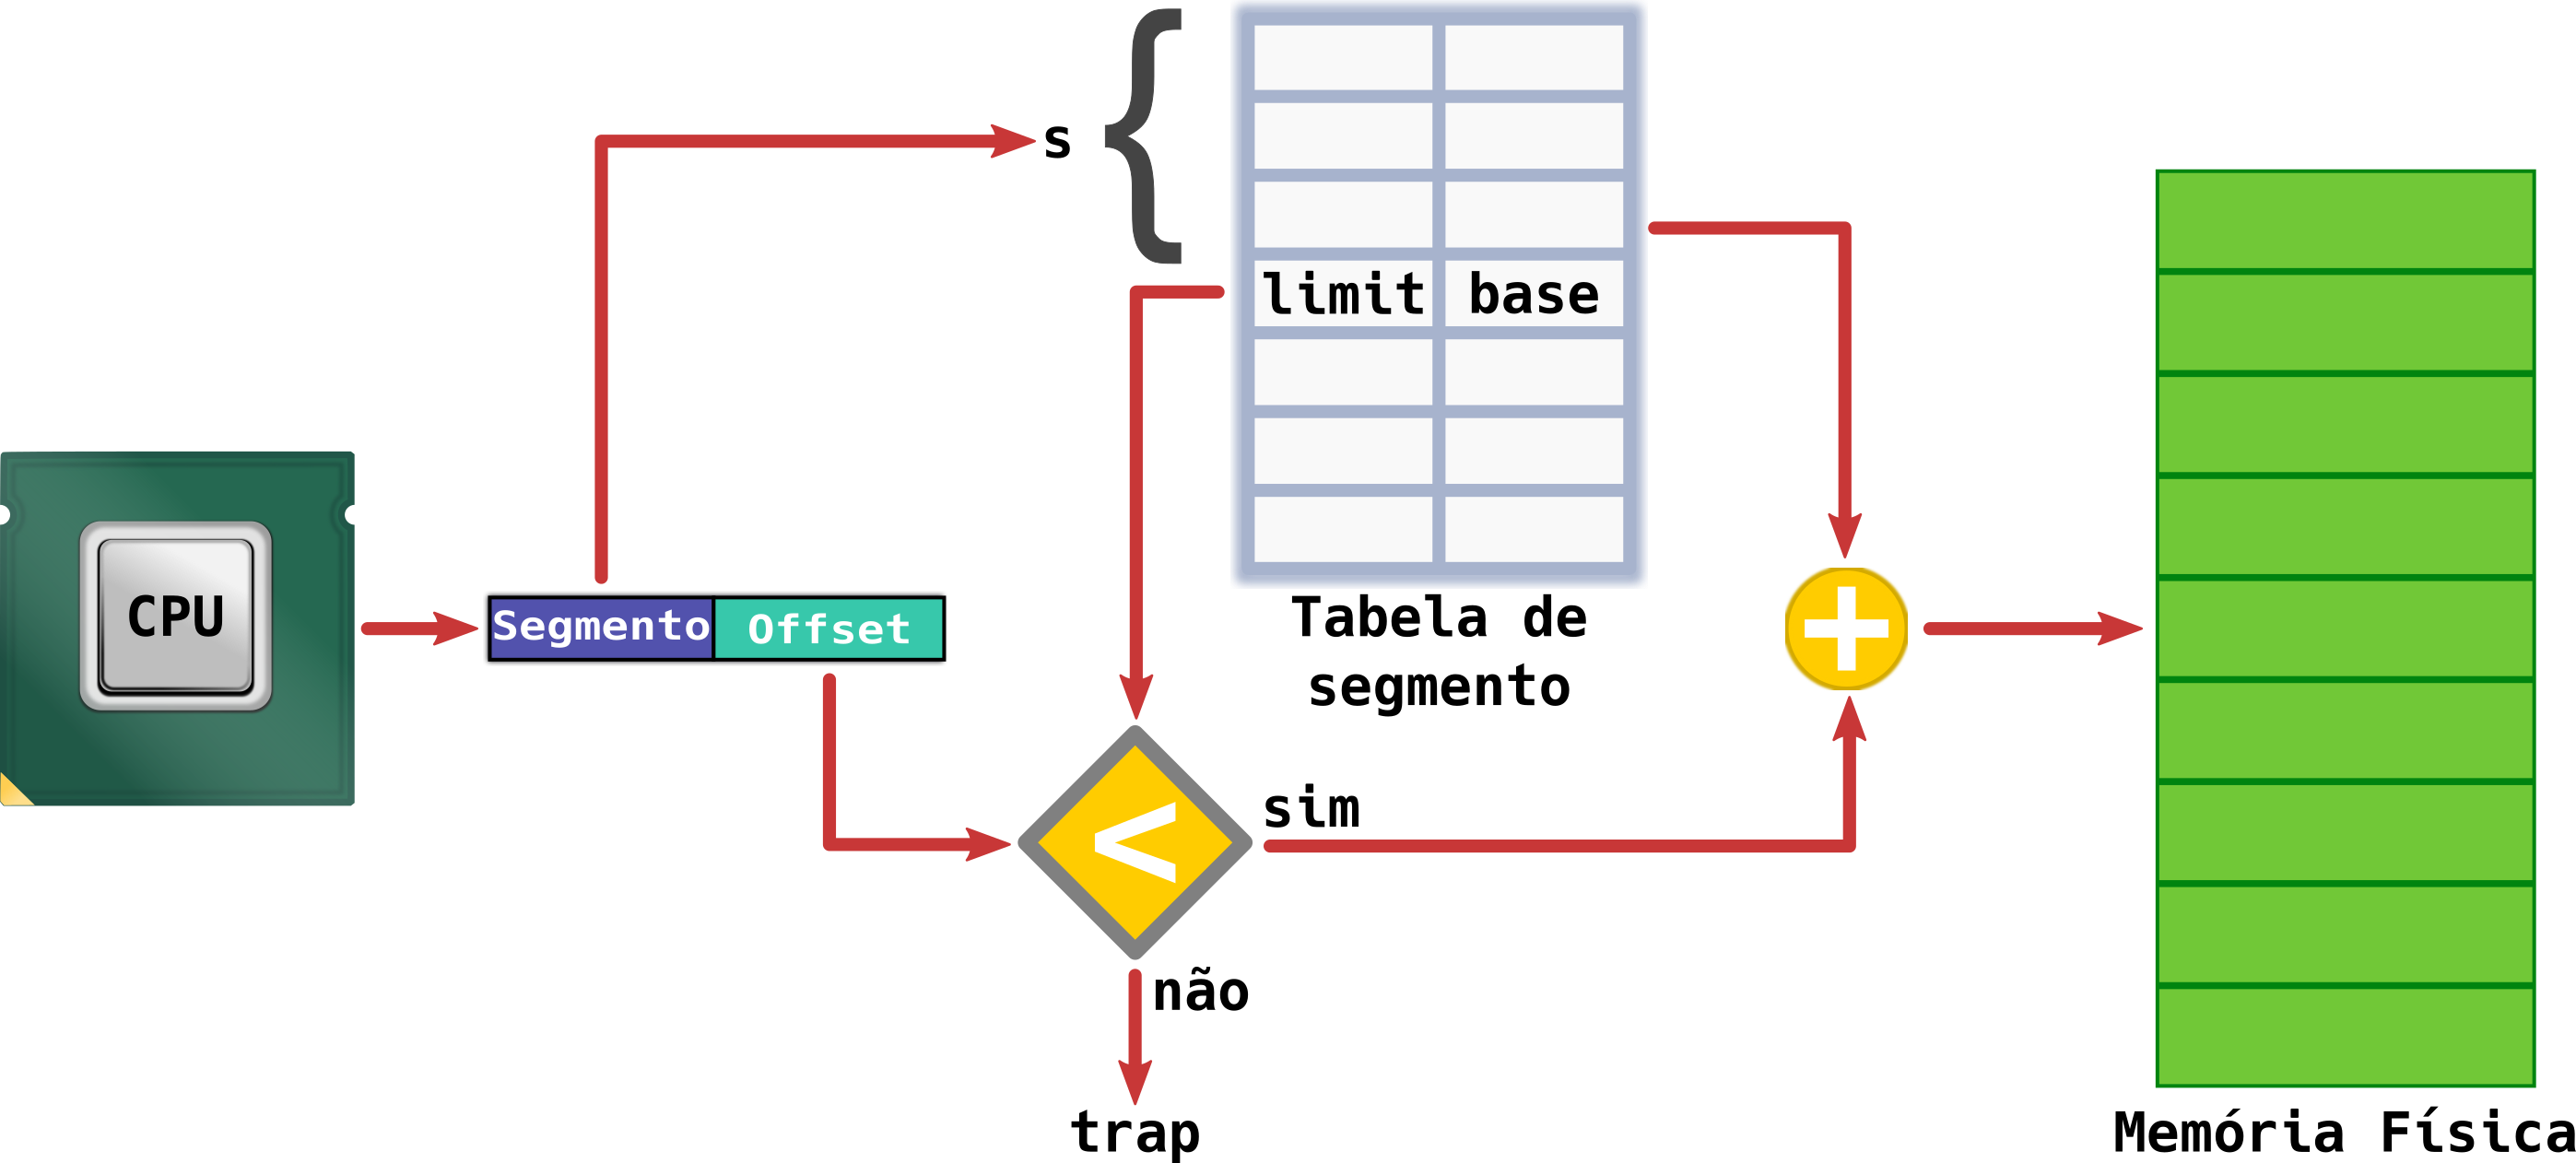
\includegraphics[width=.80\textwidth]{segmentacao} 
  \caption{Segmento de memória}
  \label{fig:memory_segment} 
\end{figure}

Tanto o modelo de segmentação quanto o de paginação tem suporte de hardware. O
Windows é um SO que faz uso do modelo de segmentação, enquanto o MacOS e o
GNU/Linux usam a paginação. Como a CPU costuma dar suporte para ambos os
esquemas, os SOs podem utilizar esses mecanismos para executar aplicações de
outros SOs. Por exemplo, o Wine executa aplicações Windows no Linux utilizando
parte dos recursos de segmentação fornecidos pela CPU.

\subsection{Outros Mecanismos de Memória}
\label{sec:outros_mecanismos_memoria}

Os microprocessadores ARM oferecem alguns recursos adicionais atrelados a
tabelas de tradução, dentre eles destacam-se os campos de permissão e o domínio
(estes trabalham juntos). Cada região de memória definida na tabela de tradução
é controlada por um domínio que é especificado em um campo da tabela, no total
existem 16 desses domínios diferentes disponíveis para utilização
\cite{armdeveloperguide}. O aspecto mais interessante em se utilizar domínios
está no comportamento que este apresenta caso ocorra alguma tentativa de acesso
da memória, dentre elas:

\begin{itemize}
  \item O acesso pode ser permitido se o conjunto de permissões presentes na
        tabela permitir o acesso;
  \item Gerar uma falta de domínio;
  \item O acesso é permitido de acordo com a permissão.
\end{itemize}

Normalmente quem faz a solicitação de acesso a memória é a CPU em favor de
algum processo, então a MMU precisa proceder com algumas verificações que
consiste em três passos:

\begin{enumerate}
  \item A MMU verifica o número do domínio encontrado na tabela de tradução;
  \item Com base no número obtido do passo anterior, a MMU verifica a permissão
        de acesso no registrador de controle de acesso;
  \item De acordo com o valor encontrado no registrador de domínio de acesso a
        MMU pode tomar as seguintes decisões:
  \begin{itemize}
    \item Permitir o acesso;
    \item Bloquear o acesso;
    \item Verificar a permissão de acesso em uma tabela de tradução.
  \end{itemize}
\end{enumerate}

Nesse contexto o SO pode tomar algumas decisões para cada aplicação; dentre
elas permitir, restringir ou negar o acesso para diferentes áreas da memória.
Além disso, o SO pode mudar permissões de acesso para um grande número de
regiões simultâneas. Note que o mecanismo de domínios é um recursos adicional
ao tradicional modelo de controle da memória adotado pelos SOs, ou seja, é
um recurso não fundamental mas que oferece novos recursos aos desenvolvedores.

\subsection{Uma visão prática do programa na memória}

A maioria dos conceitos apresentados até agora representam o ponto de vista
teórico dos SOs, nessa seção revisitamos e expandimos alguns dos conceitos da
perspectiva do Kernel Linux. Essa visão é relevante para o presente texto uma
vez que a maioria dos trabalhos analisados faz uso de SOs baseados no Kernel
Linux. Por fim, por uma questão de simplicidades usaremos o termo Kernel como
sinônimo de Linux nessa seção.

Para iniciar a analise, começamos por um fato interessante sobre VAS no Linux
em uma arquitetura x86: uma vez que a VAS é ativada, todo sistema é afetado
incluindo o Kernel. Por este motivo, uma porção da VAS tem que ser reservada
para o Linux de forma a manter o acesso restrito (privilégiado) e sempre
presente na memória física. Por outro lado, a VAS dos processos são movidas
constantemente de acordo com a troca de contexto e podem ser acessados pela
aplicação.

A Figura \ref{fig:vas_contexto} busca ilustrar o mapeamento da VAS levando-se
em consideração o espaço reservado para Kernel e os processos. O lado esquerdo
da figura mostra de forma detalhada a área do Kernel e os segmentos alocados
para o processo em execução (descrito na seção \ref{sec:processos-e-threads}).
A figura também demonstra a troca de contexto que ocorre entre dois processos;
repare que a VAS dos processos é alterada mas o kernel permanece constante.

\begin{figure}[!h]
  \centering
  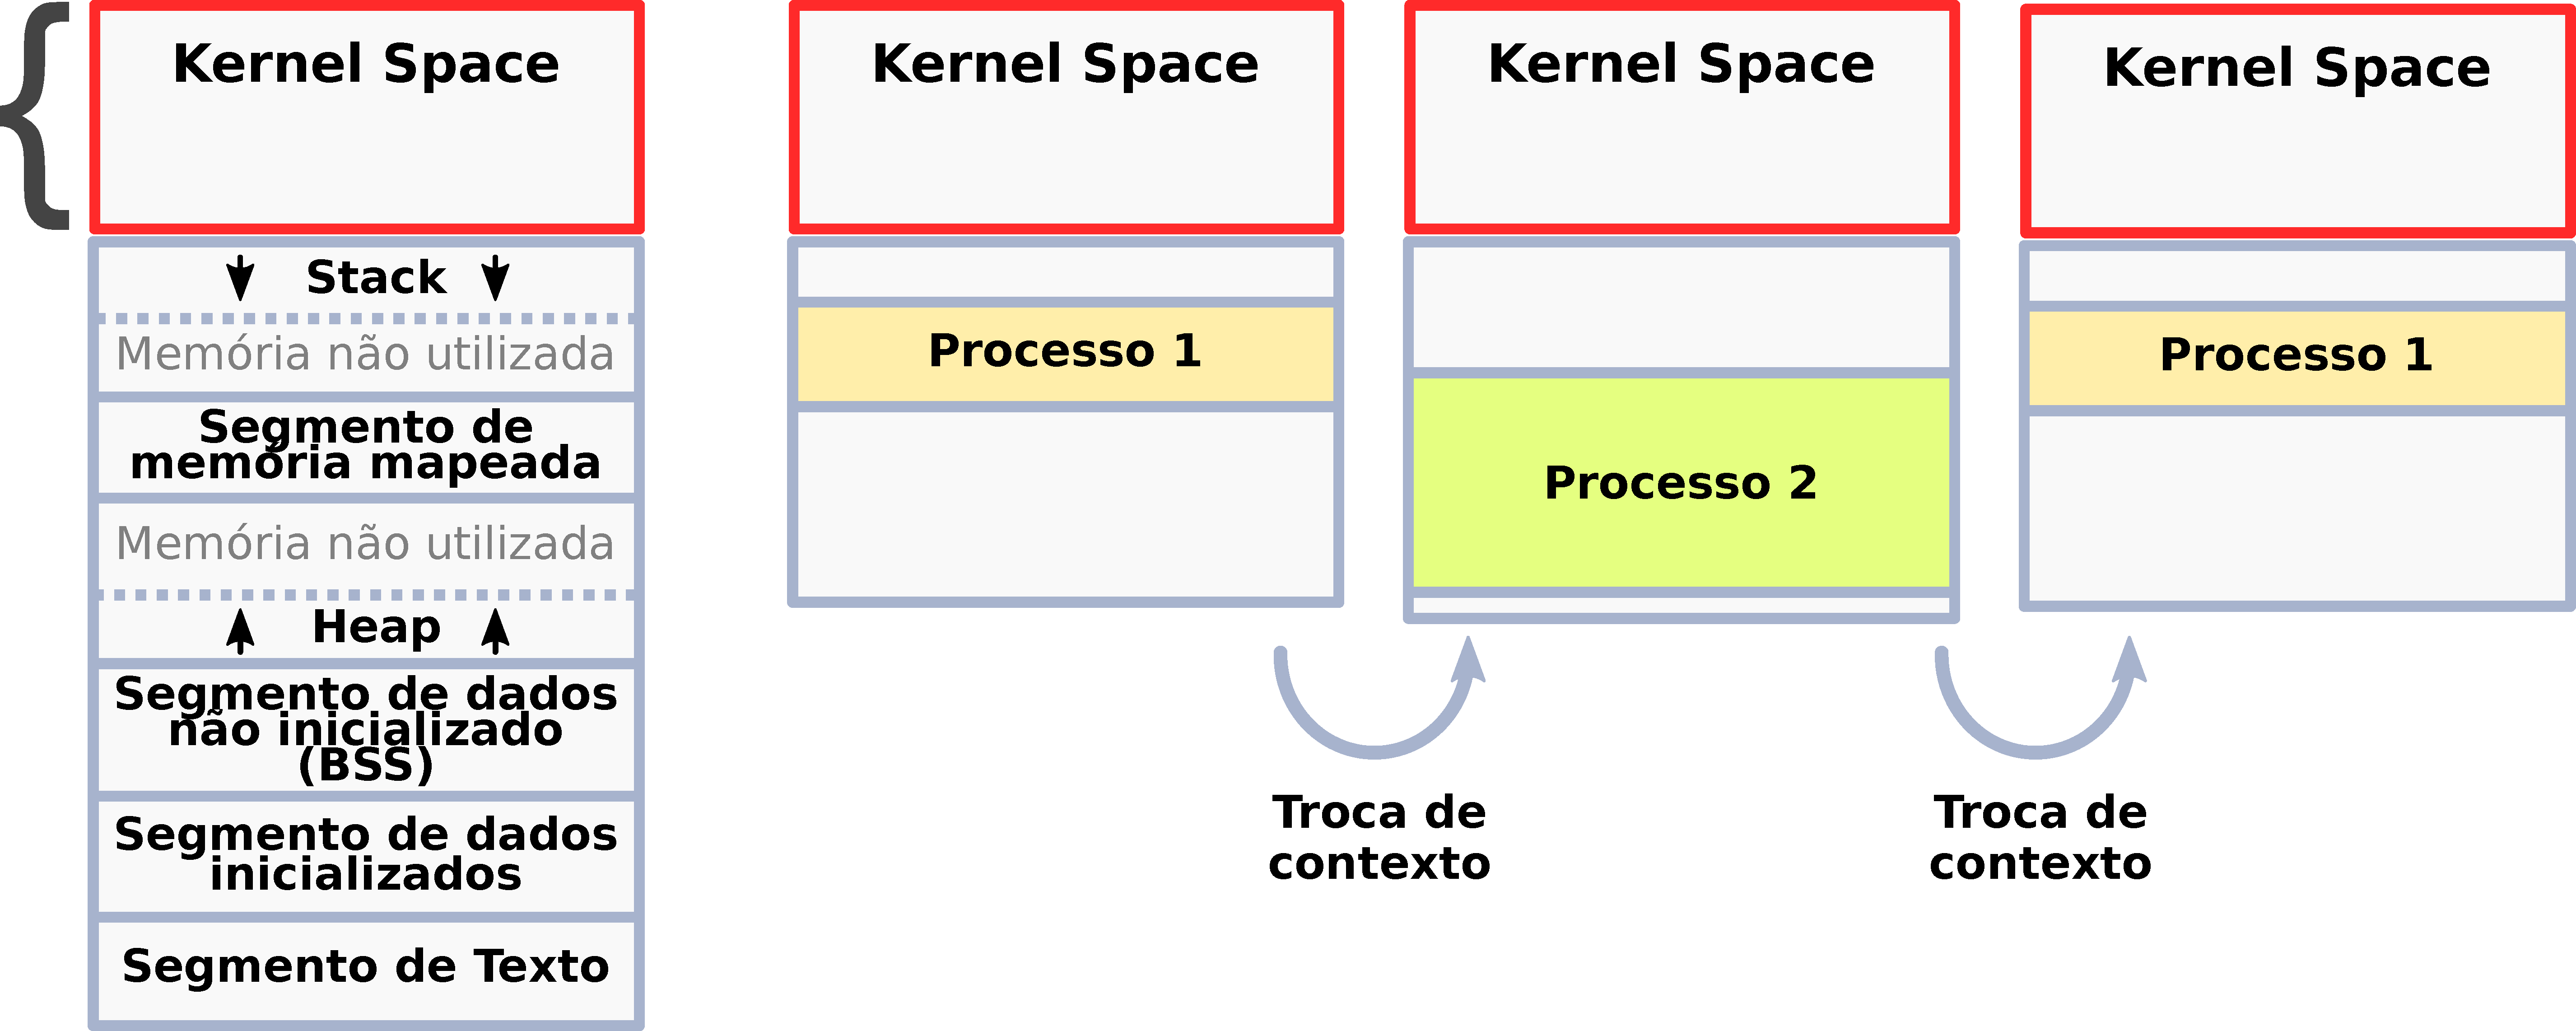
\includegraphics[width=\textwidth]{segmento_troca_contexto}
  \caption{VAS durante a troca de contexto, imagem baseada em \citep{kernel_manages_memory}}
  \label{fig:vas_contexto}
\end{figure}

O \textit{layout} de uma VAS é o mesmo para todos os processos, note que isso
cria brechas de segurança uma vez que um atacante que compreenda essa informação
pode explorar a mesma com o objetivo de realizar ataques. Como resposta a essa
falha de segurança o Kernel implementa uma série de mecanismos de randomização
conhecidos como ASLR, KASLR and KARL~\citep{aslr, kaslr}. Tal recurso faz com
que a sequência dos segmentos sejam randomizada a cada execução do processo,
tornando o sistema mais seguro.

Como explicado na Seção \ref{sec:processos-e-threads}, toda vez que uma função
é chamada, um \textit{stack frame} novo é criado e inserido na \textit{stack}.
Essa \textit{stack} começa com um tamanho pré-definido (8 Mb) que normalmente é
o suficiente para a maioria das aplicações. Contudo esse limite pode ser
ultrapassado, consequentemente o Kernel faz uma operação para expandir o
tamanho da stack. Se o tamanho máximo da \textit{stack} for atingido, então um
\boldAndIndex{stack overflow} ocorre. Vale observar que depois que a \textit{stack} é
aumentada ela pode ser encolhida.

Ainda na Figura \ref{fig:vas_contexto}, note que o processo possuí um conjunto
de segmentos que mapeia arquivos diretamente na memória para o rápido acesso;
tal segmento recebe o nome de \boldAndIndex{segmento de memória mapeada}. O uso mais
interessante de tal segmento, do ponto de vista do kernel, é o
\boldAndIndex{mapeamento anônimo} que é realizado pelo programa para obter espaço
para dados; o uso comum para essa região é o mapeamento das bibliotecas
dinâmicas. A biblioteca C (\textit{libc}) utiliza esse recurso como uma forma
de otimizar grandes alocações solicitadas via \texttt{malloc()}, basicamente a
libc cria um mapeamento anonimo para tais casos.

Observando a Figura X, note que temos o \textit{heap} e como esperado esse é
manipulado pela função \texttt{malloc()} na maior parte do tempo. Todo processo
inicia com um pequeno espaço para o \textit{heap} e que é manipulado pela libc,
geralmente o tamanho fornecido é suficiente. Contudo, se o programa demandar
mais memória, então a biblioteca faz uma chamada de sistema para a função
\texttt{brk()} que expande o tamanho da \textit{heap}. Na Figura X o BSS é um
segmento anonimo, uma vez que esse armazena variáveis estáticas não
inicializadas (valores não disponíveis no código fonte). Ao contrário do BSS, a
região de Data mapeia um arquivo uma vez que esse mantém o conteúdo das
variáveis estáticas mapeadas do código. A mesma ideia é valida para a região do
\textit{text}.

\begin{figure}[!h]
  \centering
  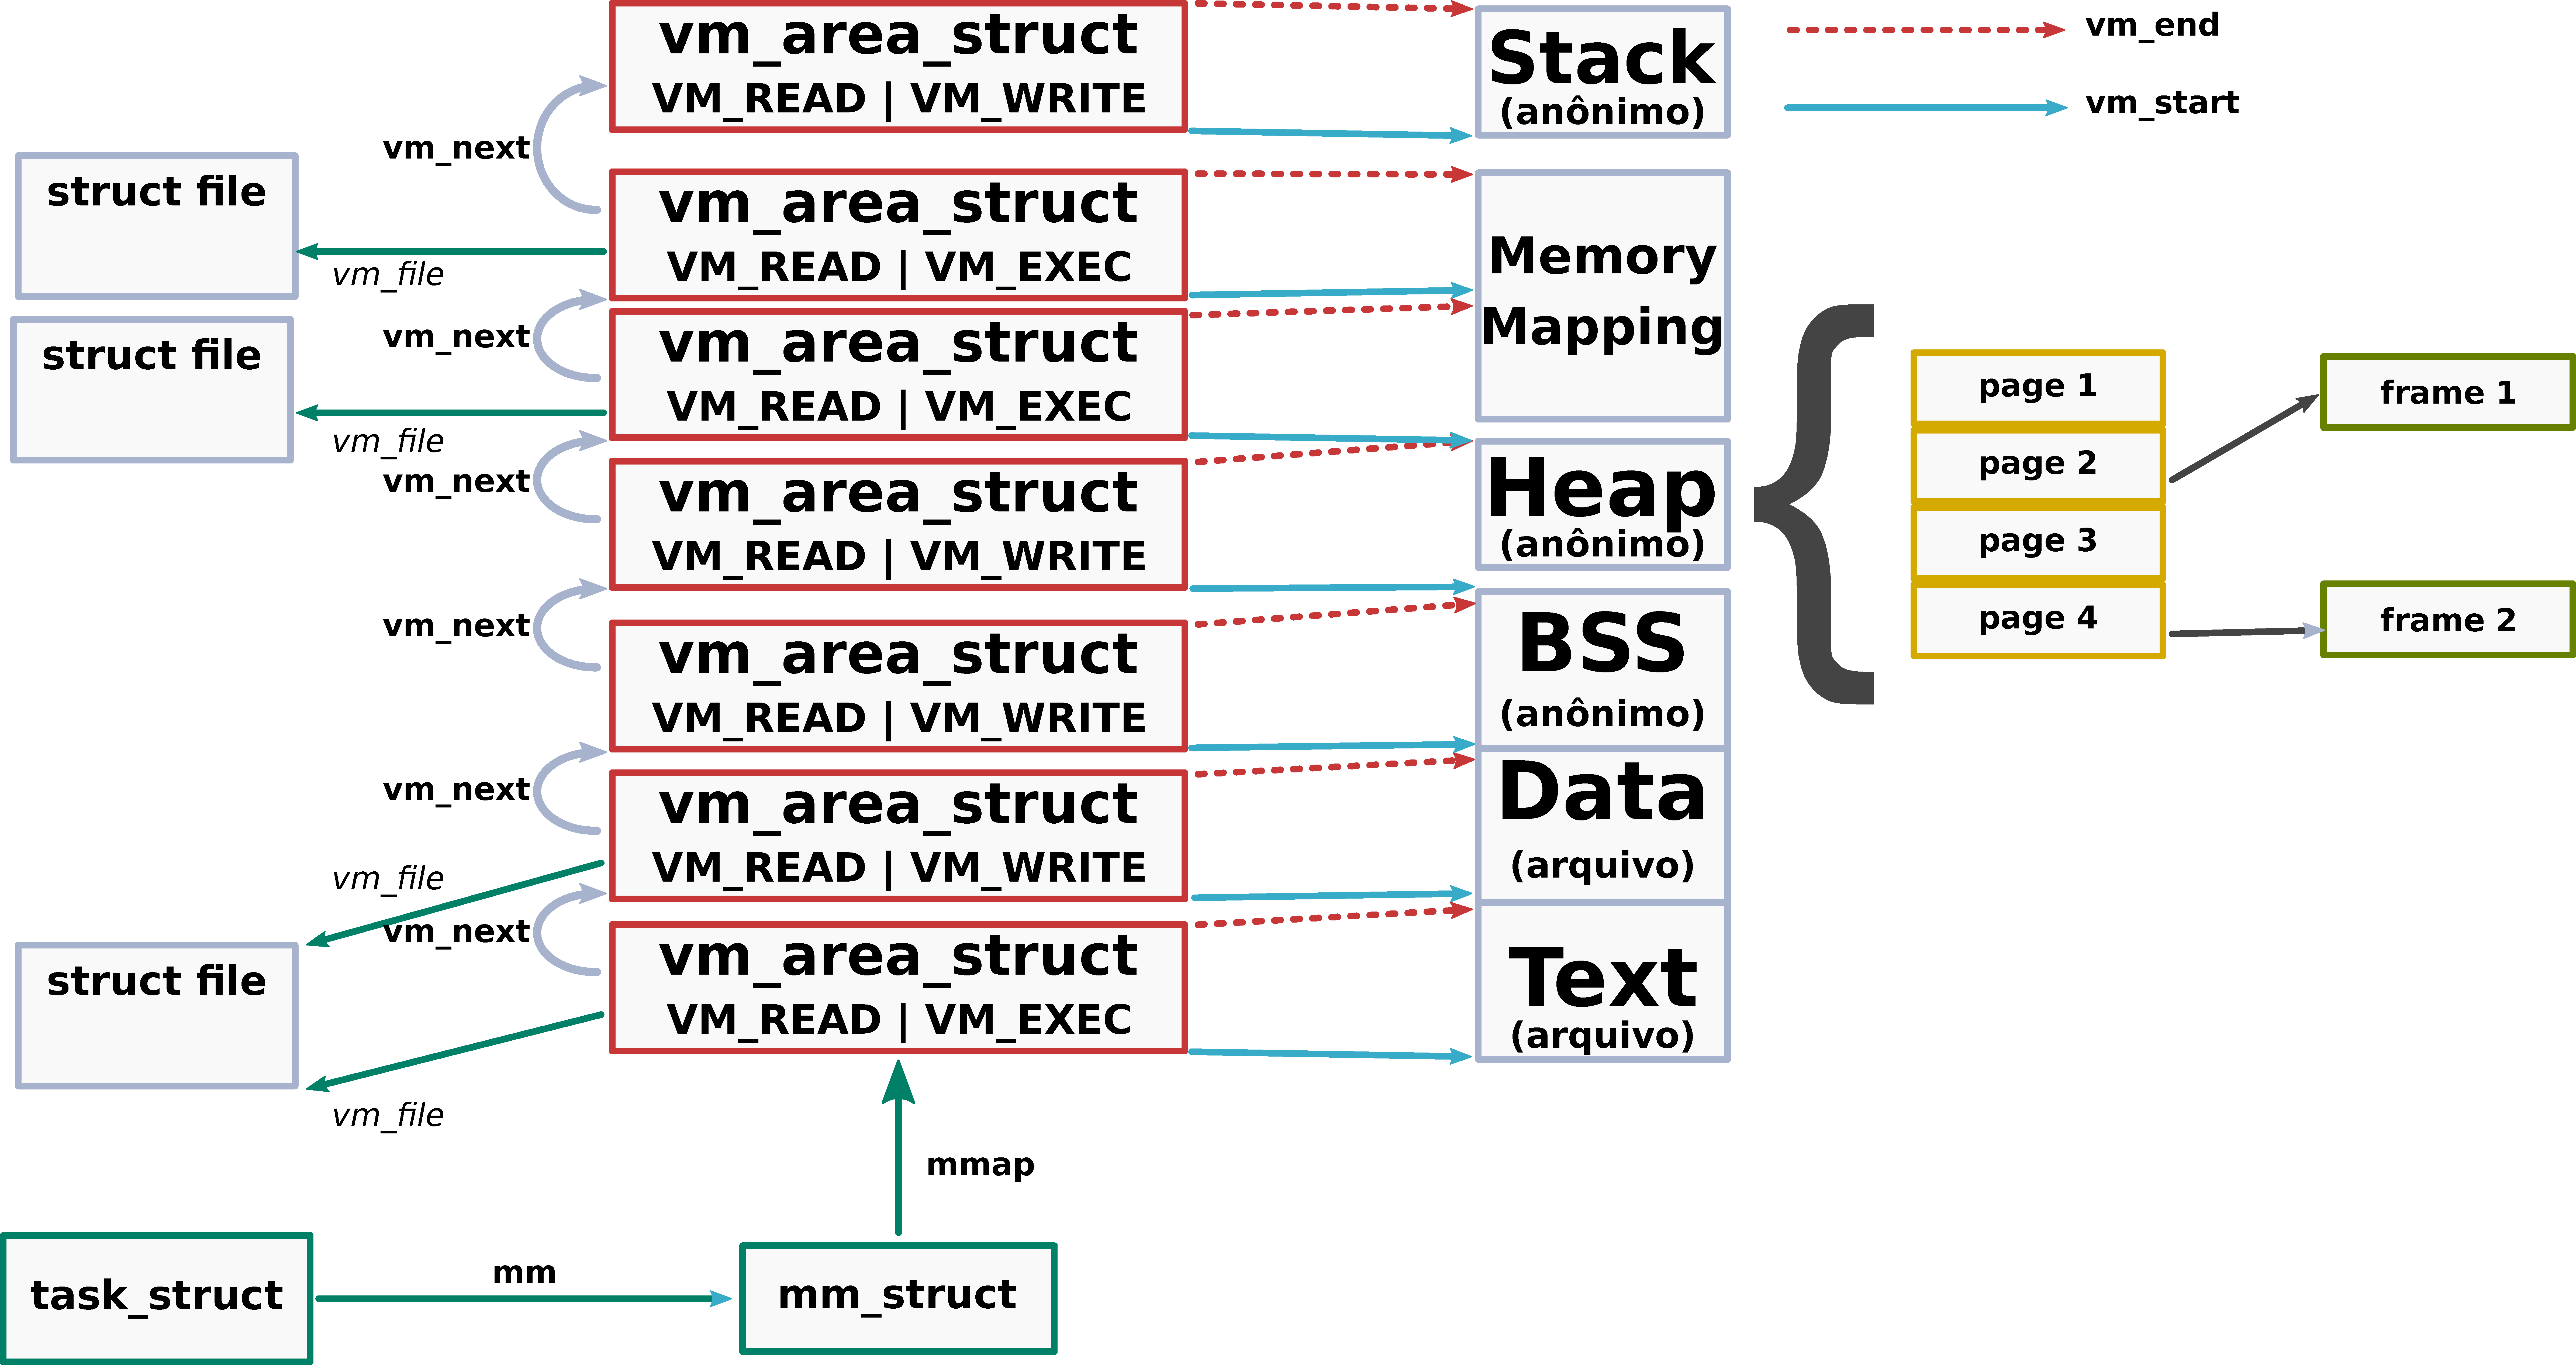
\includegraphics[width=\textwidth]{kernel_manages_memory}
  \caption{Visão interna do gerenciamento da memória, imagem baseada em \citep{kernel_manages_memory}}
  \label{fig:kernel_manages_memory}
\end{figure}

Para entender na prática como o Kernel gerencia a memória, vamos expandir os
conceitos da Figura X para a forma como eles são implementado no Linux. Veja a
Figura \ref{fig:kernel_manages_memory} ilustrando as estruturas de dados usadas
pelo Linux e as suas ligações. No Kernel a estrutura responsável por manter
todas as informações do processo (i.e.; PCB) chama-se \texttt{task\_struct},
essa tem um ponteiro para outra estrutura de dados chamada de
\texttt{mm\_struct}; por sua vez tal estrutura de dados mantém uma lista ligada
para estruturas do tipo \texttt{vm\_area\_struct} (ou \boldAndIndex{virtual memory
area - VMA}). A VMA em conjunto com a tabela de páginas orquestram o
gerenciamento do programa na memória.

Uma VMA consiste de um intervalo de endereços virtuais contíguos e sem
sobreposição com algumas \textit{flags} de controle de acesso associado a si. A
informação se a VMA é anonima ou não, vem do campo \texttt{vm\_file} (se esse
estiver vazio, então a área é anonima). Repare na figura que cada segmento
corresponde a uma VMA com exceção do segmento de mapeamento que pode ter mais.

Lembre-se que a VAS é dividia em páginas, por esse motivo o tamanho de uma VMA
deve ser um múltiplo de uma página. Toda vez que um acesso na memória é feito,
a tabela de páginas do processo é consultada e cada entrada dessa tabela é
descrita por uma série de metadados que descreve a região de memória. Cada
entrada recebe o nome de \boldAndIndex{entrada da tabela de páginas} (\textit{Page
Table Entry}) ou simplesmente PTE. A Figura \ref{fig:pte} ilustra como a
entrada é representada. Sem entrar em detalhes nos campos (a figura é
autoexplicativa), podemos concluir que uma página virtual é a unidade de
proteção da memória por que todos os bytes dela compartilham os bits User/Root
e Leitura/Escrita.

\begin{figure}[!h]
  \centering
  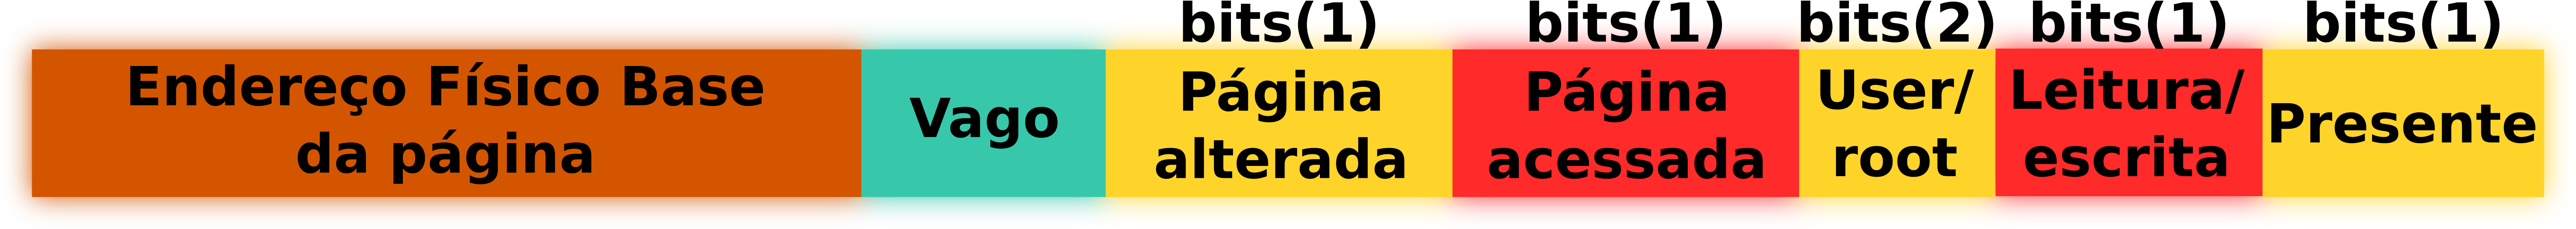
\includegraphics[width=\textwidth]{pte}
  \caption{Entrada da tabela de páginas}
  \label{fig:pte}
\end{figure}

Por fim para exemplificar como esses mecanismos estão relacionados, veja a
Figura \ref{fig:malloc_linux}. Nesse exemplo, temos um programa com algumas
paginas já mapeada para uma memória física. A aplicação decide alocar mais
memória por meio da função \texttt{malloc()}, por sua vez, uma chamada para
\texttt{brk()} é feita e o kernel atualiza o VMA do \textit{heap} com o tamanho
solicitado e retorna o ponteiro. Na prática, nenhum endereço físico foi alocado
e enquanto o programa não acessar a região alocada nenhum frame é criado. Na
primeira tentativa de acesso ocorre uma falha de página e a função
\texttt{do\_page\_fault()} é chamada. Se o processo atender as permissões
indicadas na PTE, então o kernel aloca e associa o frame a página.

\begin{figure}[!h]
  \centering
  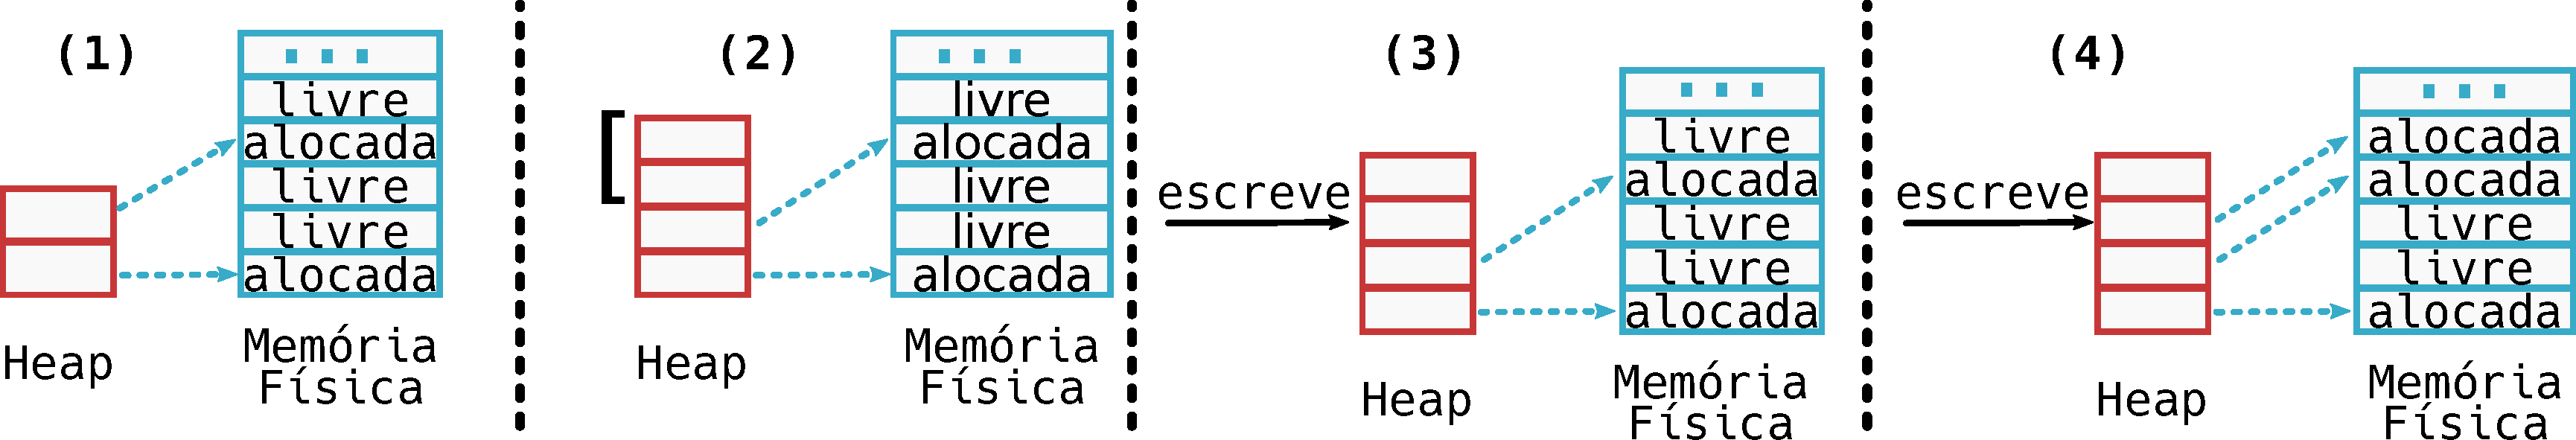
\includegraphics[width=.70\textwidth]{malloc}
  \caption{Alocação de memória com \texttt{malloc()}, imagem baseada em \citep{anatomy_program_mem}}
  \label{fig:malloc_linux}
\end{figure}

\section{Aspectos gerais relativos a abstração de processos}

\subsection{Chamadas de Sistema}
% TODO: Fazer a distinção entre user space e kernel space

\cite{silberschatz} apresenta diversas perspectivas sobre os SOs, dentre elas
destaca-se a ideia de que um SO fornece serviços para tornar as tarefas de
programação mais simples para os desenvolvedores. Partindo de tal concepção
podemos notar os seguintes serviços: controle sobre a execução de um programa,
operações de I/O, manipulação de sistemas de arquivos, comunicação, detecção de
erros, alocação de recursos, dentre outros. Dado a vasta quantidade de serviços
oferecidos, deve-se ter a seguinte pergunta em mente: qual mecanismo utilizado
pelo SO para dar acesso para todos os serviços? A resposta é simples: chamadas
de sistema (também conhecidas por \emph{system call} ou \emph{syscall}).

De forma geral, podemos dizer que uma chamada de sistema consiste em uma API de
baixo nível que permite que uma aplicação executando no espaço de usuário
(\emph{user space}) faça uma requisição de baixo nível para o SO. Por sua vez,
esse pedido é rigorosamente validada pelo SO que pode permitir executar a
operação até o fim, retornando o que a aplicação solicitou; ou pode negar caso
encontre uma inconsistência. Na prática, esse tipo de operação consiste em uma
simples chamada de função que é tratada pelo SO. Normalmente cada
\emph{syscall} tem um número associado a si, com isso o SO consulta uma tabela
que identifica a função que deve ser chamada. Além disso, passar parâmetros
para esse tipo de função pode depender da arquitetura e de outros detalhes.
Para tentar esconder toda a complexidade por trás desse tipo de operação,
muitas vezes são escritas bibliotecas que encapsulam esse tipo de chamada. O
exemplo mais emblemático é a \emph{libc} que oculta vários detalhes de baixo
nível como a leitura e escrita de um arquivo.

Para ilustrar como esse conceito funciona na prática, veja a Figura
\ref{fig:userspace_kernelspace} mostrando um simples programa que pede o seu
PID para o SO (exemplo baseado em \cite{syscallex}). O programa executando está
na memória e esse tem o seu \emph{Address Space} devidamente inicializado; ao
invocar a função \texttt{getpid()}, o seu fluxo de execução é levado para a
\emph{libc}. Por sua vez a \emph{libc} faz algumas operações, tal qual alocar
espaço na memória para fazer cache do PID. Quando a \emph{libc} estiver pronta
ela finalmente faz a chamada para o sistema. Note que nessa etapa ocorre uma
mudança de um modo de execução menos privilégiado (\emph{ring 3}) para um modo
privilégiado (\emph{ring 0}). Nesse momento o SO tem total controle sobre o
pedido feito e faz a verificação dos parâmetros e permissões. Se tudo ocorrer
bem, o SO se encarrega de copiar a informação pós-processada do \emph{Kernel
space} para o \emph{user space}. Por fim, a \emph{libc} salva o valor do seu
cache evitando a necessidade do SO intervir no futuro e a aplicação finalmente
recebe o seu PID.

\begin{figure}[!h]
  \centering
  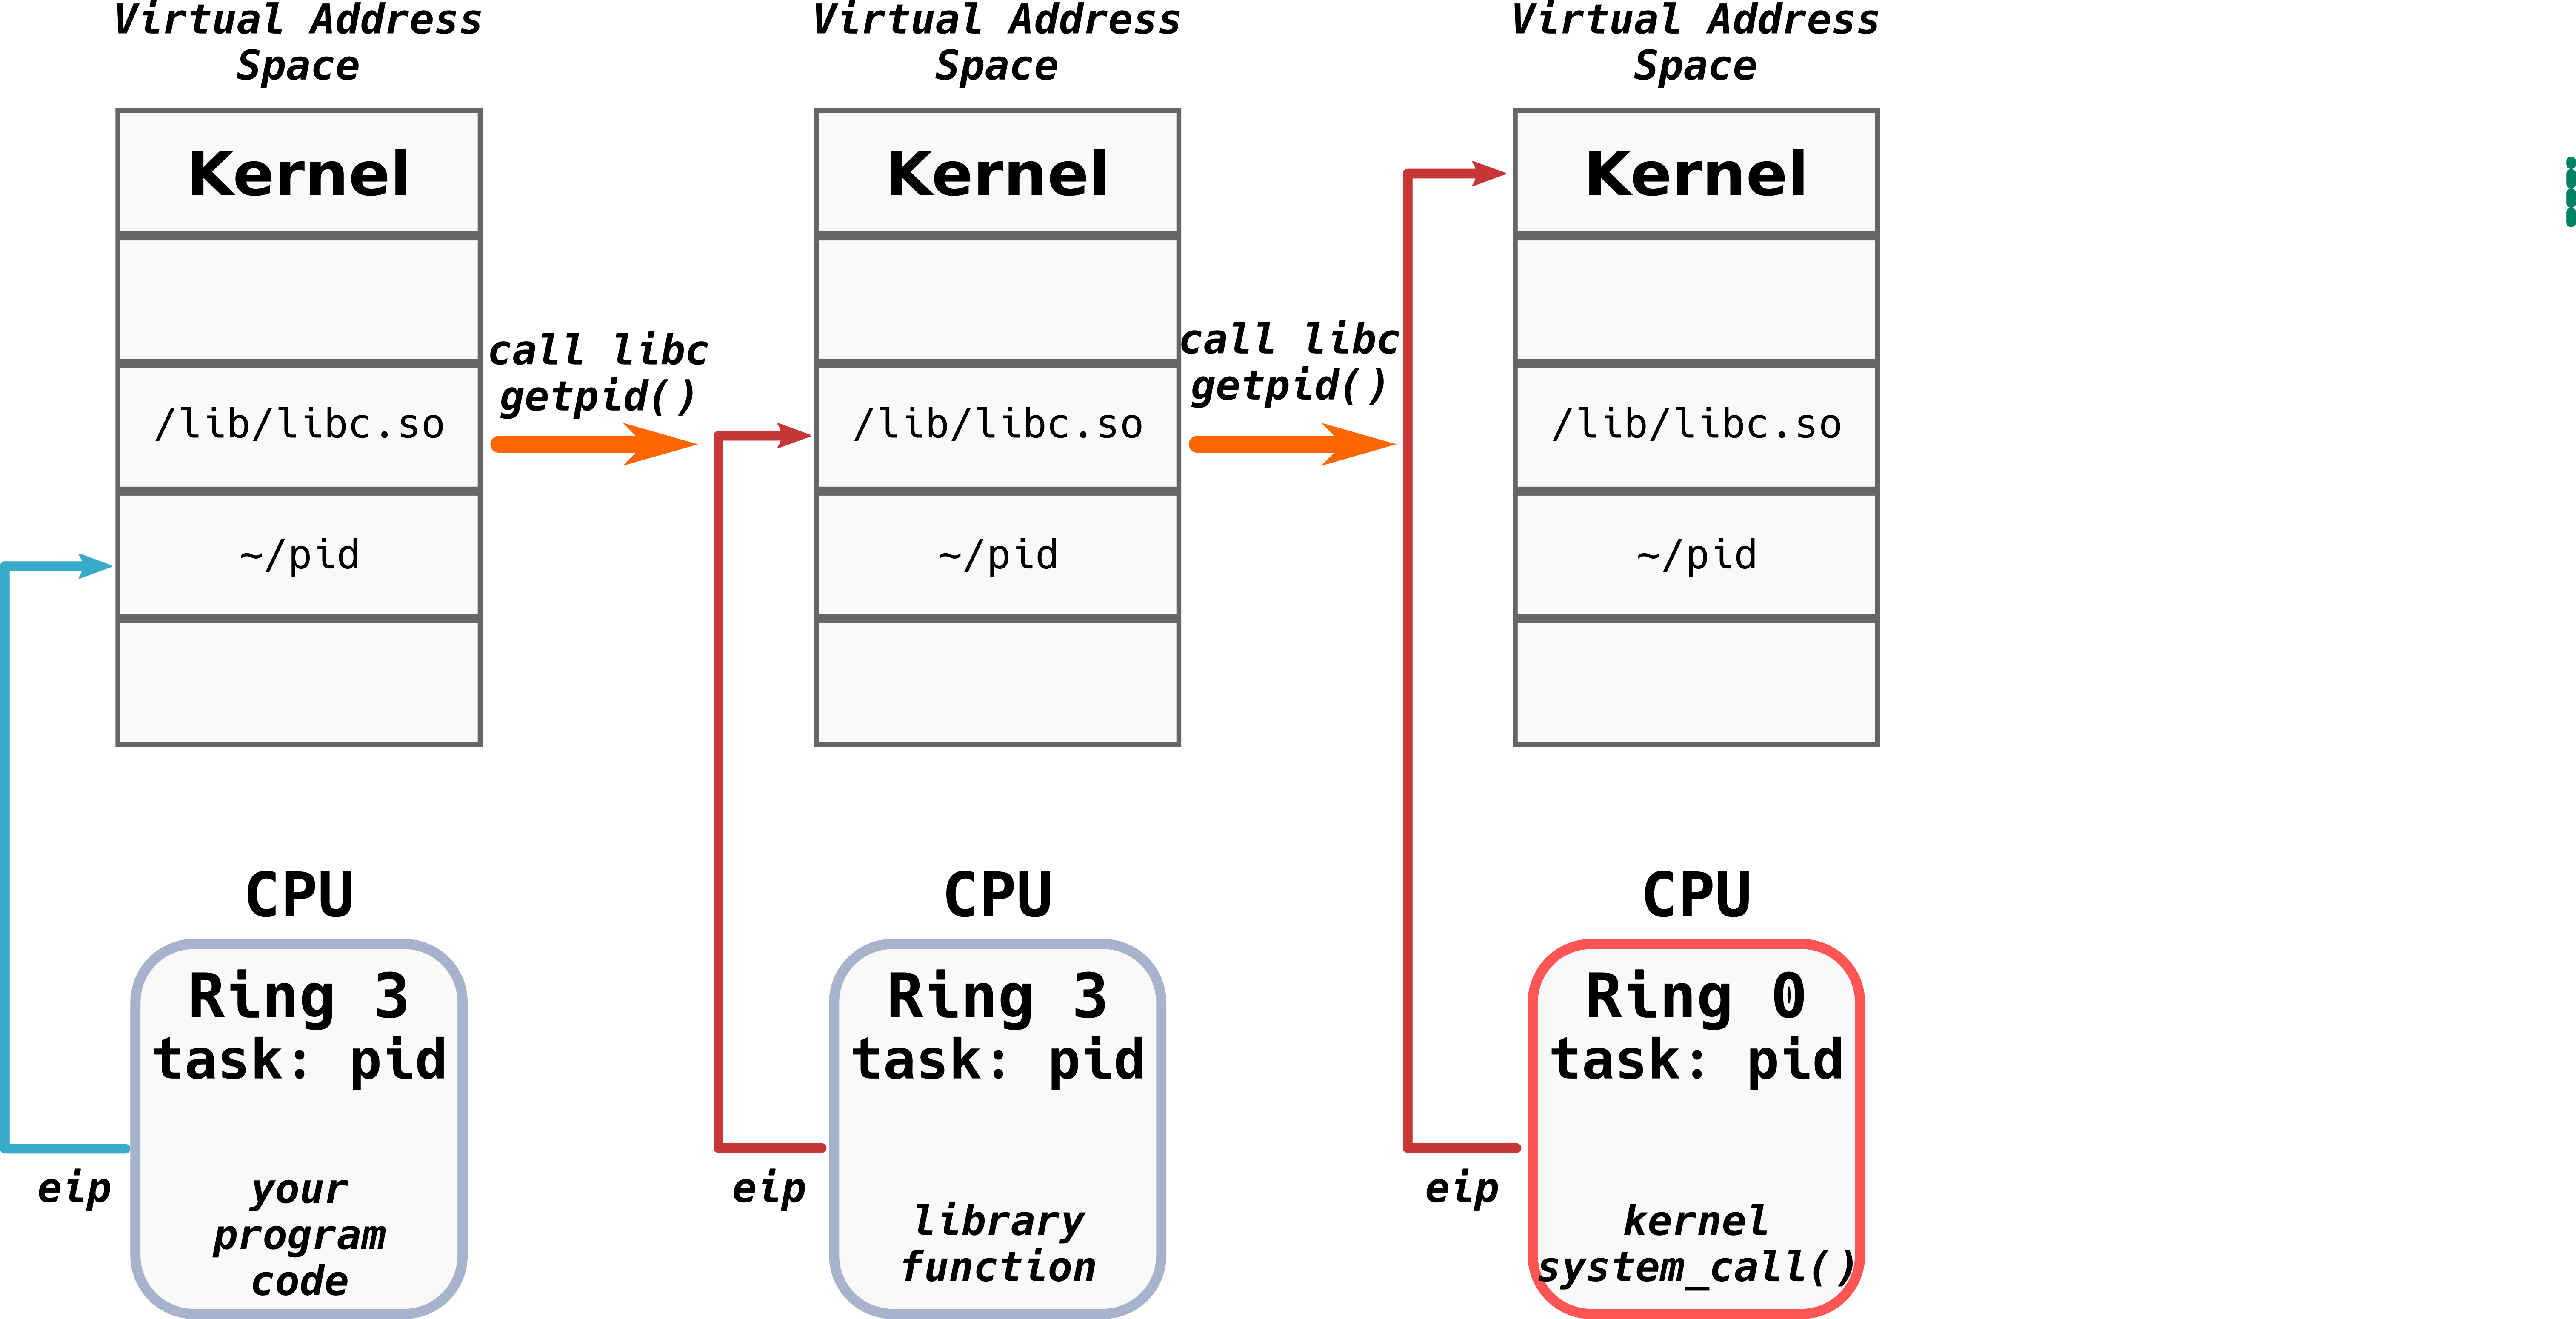
\includegraphics[width=0.8\textwidth]{userspace_to_kernel} 
  \caption{Execução do user space até o kernel space}
  \label{fig:userspace_kernelspace}
\end{figure}

\subsection{Troca de Contexto}

Em um SO de proposito geral é comum que tenhamos múltiplos processos executando
por um intervalo de tempo e após tal intervalo os processos são trocados. A
troca tem início quando uma interrupção ocorrer, seja ela porque o tempo de CPU
do processo terminou ou por qualquer outro motivo. O primeiro passo necessário
consiste em salvar todos o estado do processo em execução e em seguida carregar
o estado do novo processo na CPU. Repare que o tempo gasto na troca de processo
não produz nenhum trabalho útil sendo um mecanismo de
\textit{overhead}~\citep{silberschatz}.

Na prática a troca de contexto é bem mais complexa, por exemplo, vamos olhar de
perto e de forma breve a troca de contexto no GNU/Linux em uma arquitetura x86.
Primeiramente, todos os processos precisam compartilhar os registradores da
CPU, por esse motivo o kernel deve assegurar que todos os registradores sejam
carregados com os valores de quando o processo foi suspenso. O conjunto de
todos os dados dos registradores que devem ser carregado recebem o nome de
\boldAndIndex{contexto de hardware}~\citep{entendendo_kernel}, esse pode ser
visto como subconjunto do contexto do processo. No Linux o contexto do hardware
é armazenado na própria estrutura do processo e as demais partes são salvas na
stack do kernel mode. Toda troca de processo precisa armazenar o contexto de
hardware, por isso a \texttt{task\_struct} incluí um campo chamado de
\texttt{thread\_struct} que armazena o contexto do hardware (note que essa é
dependente da arquitetura de hardware).

Para realizar a troca de processos, o Kernel Linux realiza duas
operações~\citep{entendendo_kernel}:

\begin{enumerate}
  \item Instalar o novo espaço de endereço;
  \item Mudar o stack do Kernel mode e o contexto de hardware
\end{enumerate}

A operação de troca é extremamente dependente da arquitetura de hardware, pois
precisa ser executada de forma rápida e por isso o Linux tenta tirar proveito
de todo recurso disponibilizado pela CPU. Note que é preciso levar em
consideração os registradores que lidam com pontos flutuantes o que faz a troca
de contexto ainda mais complexa.

% Falar de PCID?
\subsection{Descritores de Arquivo}

Quando falamos de abstrações de processos é preciso levar em consideração
diversos aspectos interligado a eles, dentre eles as interações de escrita e
leitura de aquivos. Normalmente, quando um processo deseja ler ou escrever um
dado em um arquivo esse precisa passar por algumas camadas. De forma geral o
processo interage com o \boldAndIndex{sistema de arquivos} que é responsável
por fornecer um mecanismo simplificado para o processo localizar, escrever e
recuperar dados. Por sua vez, os sistemas de arquivos atuam com outras camadas
responsáveis por manter a organização e meta-dados sobre dos aquivos. Por fim,
as operações de alto nível são convertidas para instruções de baixo nível
passadas para os discos que de fato realizam as operações solicitadas.

Existe uma estrutura de dados utilizada para controlar o bloco de dados e que é
usada para leitura ou escrita, essa estrutura recebe o nome de
\boldAndIndex{inode}. Um inode contém diversas informações, dentre elas:
permissão, datas, dono do arquivo, tamanho, dentre outros. Quando um arquivo é
criado, uma estrutura de dados como o inode é criada e então o arquivo é salvo.

Quando um processo abre um arquivo, ele faz uma chamada para \texttt{open()}, em
seguida, o sistema de arquivos é acionado para encontrar o arquivo solicitado.
Para isso o \texttt{open()} primeiro procura em uma \boldAndIndex{tabela global
de arquivos} para verificar se o arquivo solicitado já está aberto. Se o
arquivo estiver presente na tabela global, então uma nova entrada em uma
\boldAndIndex{tabela local de arquivos dos processos} é feita e nela é
armazenada uma nova entrada com a posição referente ao arquivo na tabela
global. A tabela global é atualizada com a informação de que um novo processo
abriu o arquivo, basicamente um contador é incrementado para representar tal
informação . Por outro lado, se não existe uma entrada para o arquivo
solicitado na tabela global, então o mesmo é carregado e a tabela global
atualizada. A Figura \ref{fig:descritores} ilustra a operação descrita.
 
\begin{figure}[!h]
  \centering
  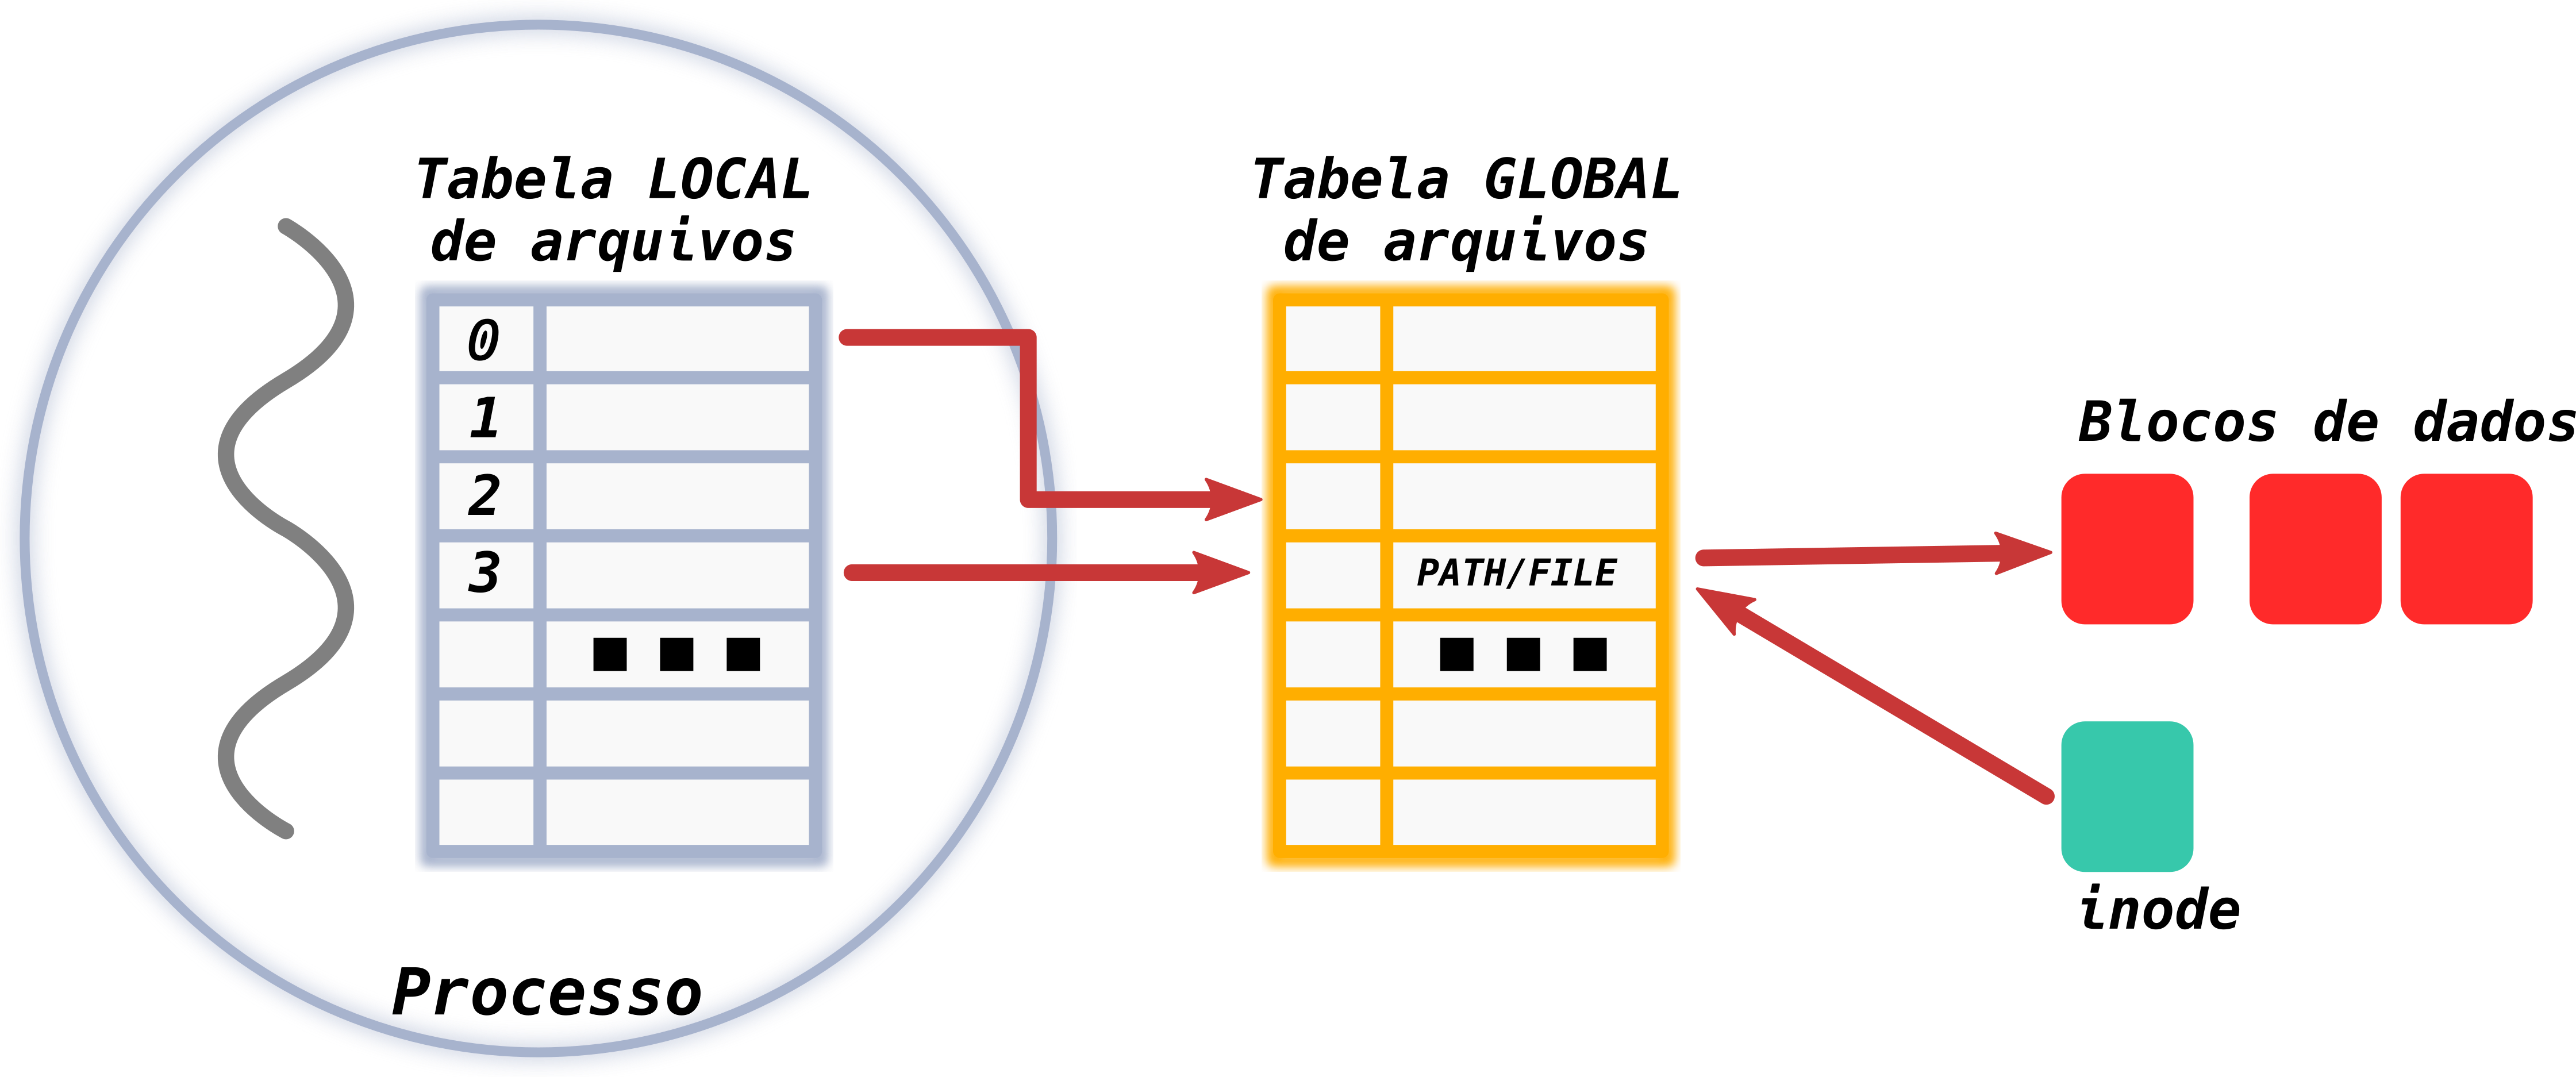
\includegraphics[width=.90\textwidth]{descritores} 
  \caption{Tabela local e global de arquivos}
  \label{fig:descritores} 
\end{figure}

Quando um arquivo é aberto por meio da função \texttt{open()}, esse retorna um
número chamado de \boldAndIndex{descritor de arquivo (file descriptor - fd)}
que nada mais é do que a posição da entrada na tabela local de processos.
Quando o processo fecha um arquivo, a entrada na tabela local é removida e o
contador de processos presente na tabela global é decrementado. Quando o
contador zera, o bloco é atualizado.

\subsection{Modelos de programação}

Além da manipulação de dispositivos de hardware, os SOs fornecem vários
recursos adicionais para o espaço de usuário, tal qual \emph{file locking} e
primitivas de segurança. Para fazer uso de tais recursos, a aplicação precisa
ser capaz de acessar as mesmas por meio de um modelo de programação coerente,
i.e., um conjunto bem estabelecido de abstrações interligadas. Um dado SO
implementa o seu modelo de programação dentro da sua própria API. Por exemplo,
tanto o GNU/Linux quanto Windows fornecem diferentes APIs de \emph{threading}
(\emph{pthread} e \emph{WindowsThreads}), mas ambos corresponde ao modelo de
programação de paralelismo.

Atualmente, a maioria dos SOs dão suporte para um grande número de modelos de
programação e suas respectivas APIs. Contudo, as aplicações mudam ao longo dos
anos e criam demandas para melhorias em áreas como camadas de segurança, opções
de otimizações e simplificação de código; esses aspectos são problemas reais.
Nesse sentido, propostas para expandir as abstrações de processos visando
introduzir novos modelos de programação são recorrentes e representam uma
interessante área para inovações.

%TODO: Mudar esse nome para algo melhor
\subsection{Aspectos de implementação}

As abstrações de processos são o ponto central no projeto de um SO moderno,
mapeando outras abstrações para ele; assim, outros serviços são suportados pelo
SO com a intenção de fornecer os mecanismos necessários para orquestrar todas
as operações dos processos (e.g., escalonador e gerenciamento de memória). Toda
estrutura necessária para gerir processos tem o lado negativo de utilizar CPU
(\emph{overhead}); para tentar mitigar essa situação, os SOs empregam um vasto
número de otimizações de hardware e software.

Mudanças em uma abstração de processos normalmente tem impactos no desempenho e
as consequências podem variar de acordo com a proposta de modificação. Por
exemplo, uma verificação adicional em uma camada pode elevar a sobrecarga no
sistema devido a uma nova característica implementada. Contudo, enquanto
extensões de processos podem degradar o desempenho, mas também podem trazer
benefícios de desempenho explorando alguma característica do hardware.

\subsection{Gerenciamento de Recursos}

Toda aplicação executando em um SO consome recursos do sistema. Frequentemente,
eles realizam boa parte do trabalho no espaço de usuário, o que requer pouca
intervenção do SO. Por exemplo, uma aplicação que faz cálculos complexos não
precisa de muito intervenção do SO. Contudo, existe uma grande quantidade de
software que demandam significante participação do SO para atingir os seus
objetivos, estendendo assim o seu consumo de recursos para o sistema. Por
exemplo, uma aplicação que utiliza recursos de rede tem várias partes das suas
atividades conduzidas pelo SO quando um pacote chega. Essa situação pode gerar
problemas devido ao controle indireto e descontrolado do uso de recursos por
atividades não confiáveis ao Kernel. Ataques do tipo \emph{Denial-of-service}
representam um exemplo da vida real que elevam o consumo do uso de recursos por
parte do SO.



\section{Device Drivers}
\label{sec:dd}

Um SO é repleto de elementos que buscam manipular e esconde a complexidade de
lidar com o hardware, portanto, tal software é consideravelmente grande e
complexo. Para tornar esse cenário ainda mais desafiador é preciso levar em
consideração que um SO deve fornecer suporte para uma infinidade de
dispositivos; a forma como os \emph{drivers} interagem com o Kernel deve ser
projetada com muito cuidado visando reduzir a complexidade e acoplamento.  O
design adotado na maioria dos SOs, é uma abordagem flexível na qual o código
para um dispositivo é mantido isolado em um \emph{driver}.

O isolamento fornecido por um \emph{device driver} é interessante, uma vez que
esse fornece um mecanismo e não uma política \cite{ddbook}. Entenda por
mecanismo como a capacidade que deve ser fornecido e por política como a forma
que a capacidade deve ser usada. Esse separação é interessante pois limita o
que um \emph{driver} deve fazer e por sua vez simplifica a implementação do
mesmo. Um exemplo disto é o \emph{Direct Rendering Managemente} do Kernel
Linux, esse fornece várias capacidades, dentre elas, a operação de trocar
\emph{framebuffers} primários com secundários; contudo é a aplicação que deve
controlar tal operação.

Por fim, é interessante ressaltar que alguns sistemas fornecem a ideia de
\boldAndIndex{Módulos carregáveis} (\textbf{loadable modules}) que significa que em
tempo de execução é possível carregar um novo \emph{device driver}. Esse tipo
de funcionalidade torna o SO mais leve e facilmente configurável. Por fim, os
módulos são extremamente flexíveis do ponto de vista da implementação uma vez
que são um código separado do núcleo do SO, respeitam a interface definida pelo
mesmo.

\section{Virtualização}
\label{sec:virtualizacao}

%TODO: Eu acho que faltou introduzir alguns dos termos básicos logo no início
% contar um pouco como funciona e acertar a fluídez do texto

A ideia de oferecer a abstrações de máquinas virtuais dentro de uma mesma
máquina é um aspiração de longa data como o emblemático trabalho de Popek e
Goldberg \cite{popek} demonstra. Este foi publicado em 1974 indicando os
requisitos necessários para a terceira geração processadores fornecessem
virtualização completa. Neste período se tinha noção de algumas das vantagens
que a virtualização por software e hardware poderia entregar. Dentre as
inúmeras vantagens da virtualização destacam-se a possibilidade de executar
aplicações legadas em um SO antigo, recursos que facilitam o processo de
desenvolvimento de software, serviços de nuvem, \emph{checkpoints}, migração de
processos, isolamento, dentre outras.

O elemento central da virtualização é o \emph{Virtual Machine Monitor (VMM)}
(também conhecido como \boldAndIndex{hypervisor}) que é responsável por criar a
ilusão de múltiplas máquinas em um mesmo hardware físico \cite{tanenbaum}.
Essas máquinas virtuais rodando sobre o mesmo hardware tem a capacidade de
executar diferentes SOs. Complementarmente a estes conceitos, existe a ideia de
máquina convidada (\emph{guest}) e máquina hóspede (\emph{host}). O primeiro
refere-se ao SO que está executando sobre o VMM e o segundo refere-se a máquina
que está executando sobre o hardware com privilégios.

Um dos objetivos da virtualização consiste em permitir que um SO inicialize
como se estivesse dando boot em uma máquina real. Para que isso seja possível é
preciso emular o hardware de forma que o \emph{guest} não perceba que está em
um mecanismo simulado; ao mesmo tempo este processo deve ocorrer de forma
eficiente. Em 1974, \citep{popek} sugeriram alguns requisitos para que os
hardware modernos dessem suporte completo para virtualização, esses conceitos
são amplamente implementados nos processadores modernos. Basicamente os autores
destacam que três dimensões que devem ser consideradas para fornecer a
virtualização completa no nível dos processadores: segurança, fidelidade e
eficiência.

No que tange o assunto segurança, o VMM deve ter total controle sobre os
recursos virtualizados. Uma opção é utilizar um interpretador que intercepta
cada instrução e realiza exatamente o que a instrução precisa. Algumas
instruções podem ser executadas diretamente, mas outras não, por exemplo, não
deve ser possível para a máquina \emph{guest} desativar as interrupções de toda
a máquina \cite{tanenbaum}. Para contornar tal situação, o o SO \emph{guest}
deve ter a ilusão de que as interrupções estão desativadas.

Do ponto de vista da fidelidade, o comportamento do programa executando na
máquina virtual deve comportar-se de forma idêntica a se estivesse executando
diretamente no hardware. Na prática existem várias complicações associadas a
este requisito que levam a categorização das instruções utilizadas pela CPU em
três grupos de diferentes:

\begin{itemize}
  \item \boldAndIndex{Instruções sensíveis}: CPUs que fornecem \emph{user mode} e
        \emph{kernel mode} apresentam instruções comuns para ambos os modos de
        operação, mas que tem comportamentos diferentes dependendo de cada modo
        de operação no qual a instrução é executada;
  \item \boldAndIndex{Instruções privilégiadas}: São instruções que geram uma
        \emph{trap} quando executado no modo usuário, mas que não geram
        \emph{trap} em modo Kernel;
  \item \boldAndIndex{Instruções de controle de fluxo sensíveis}: São aquelas que
        tentam mudar a configuração de algum recurso do sistema.
\end{itemize}

Se você tentar fazer algo em modo usuário que você não deveria ser capaz de
fazer, o hardware deve capturar essa ação; em outras palavras, Popek e Goldberg
mostraram que uma máquina é virtualizavel se o conjunto de instruções sensíveis
é um subconjunto das instruções privilégiadas. Apesar de parecer um conceito
simples, levaram-se vários anos para que as CPUs incorporassem tais definições
e assim oferecessem um adequado suporte de hardware para a virtualização.

O suporte completo para a virtualização em hardware foi resolvido apenas em
2005 pela Intel \cite{uhlig} com uma tecnologia chamada \boldAndIndex{Virtualization
Technology (VT-x)}. A AMD tem uma solução parecida chamada \boldAndIndex{Secure
Virtual Machine (SVM)}. A ideia básica é criar um invólucro no qual a máquina
virtual pode executar um SO \emph{guest} iniciado dentro deste recipiente, o SO
contínua lá até que provoque uma \emph{trap} que faz com que o VMM tenha que
lidar com a situação. O conjunto de instruções que provocam uma \emph{trap} são
controlados por um conjunto de bits na qual o VMM tem acesso, essa extensão
torna possível a execução clássica de uma máquina virtual baseada em
"interrupção-e-emulação" \cite{tanenbaum}.

Do ponto de vista da eficiência, a virtualização deve fazer com que a maior
parte do código executado pelo SO \emph{guest} não sofra interferência do VMM.
Uma das abordagens utilizada antes de se ter o hardware de virtualização foi a
adoção de técnicas na qual o hypervisor interceptava as instruções e as
reescrevia em tempo de execução com uma sequência de código considerada segura.
Esse mecanismo permitia substituir instruções sensíveis, mas não privilégiadas;
tal técnica ficou conhecida como \boldAndIndex{tradução binária} e demostrou-se
extremamente eficiente devido ao seu sofisticado mecanismo de \emph{cache}.

% TODO: Falar dos tipos de hypervisor
%FIGURA X

\subsection{A tecnologia VT-x}
\label{sec:vtx}

Em 2005 Uhlig \citep{uhlig} apresentaram a tecnologia de virtualização adotada
pela Intel para fornecer a virtualização completa no nível do processador. Na
Figura \ref{fig:vt-x_flow} podemos notar os elementos presentes em tal
tecnologia e como eles interagem, dois novos modos de operações foram
introduzidos nas CPUs: \emph{VMX non-root} e \emph{VMX root}.

\begin{figure}[!h]
  \centering
  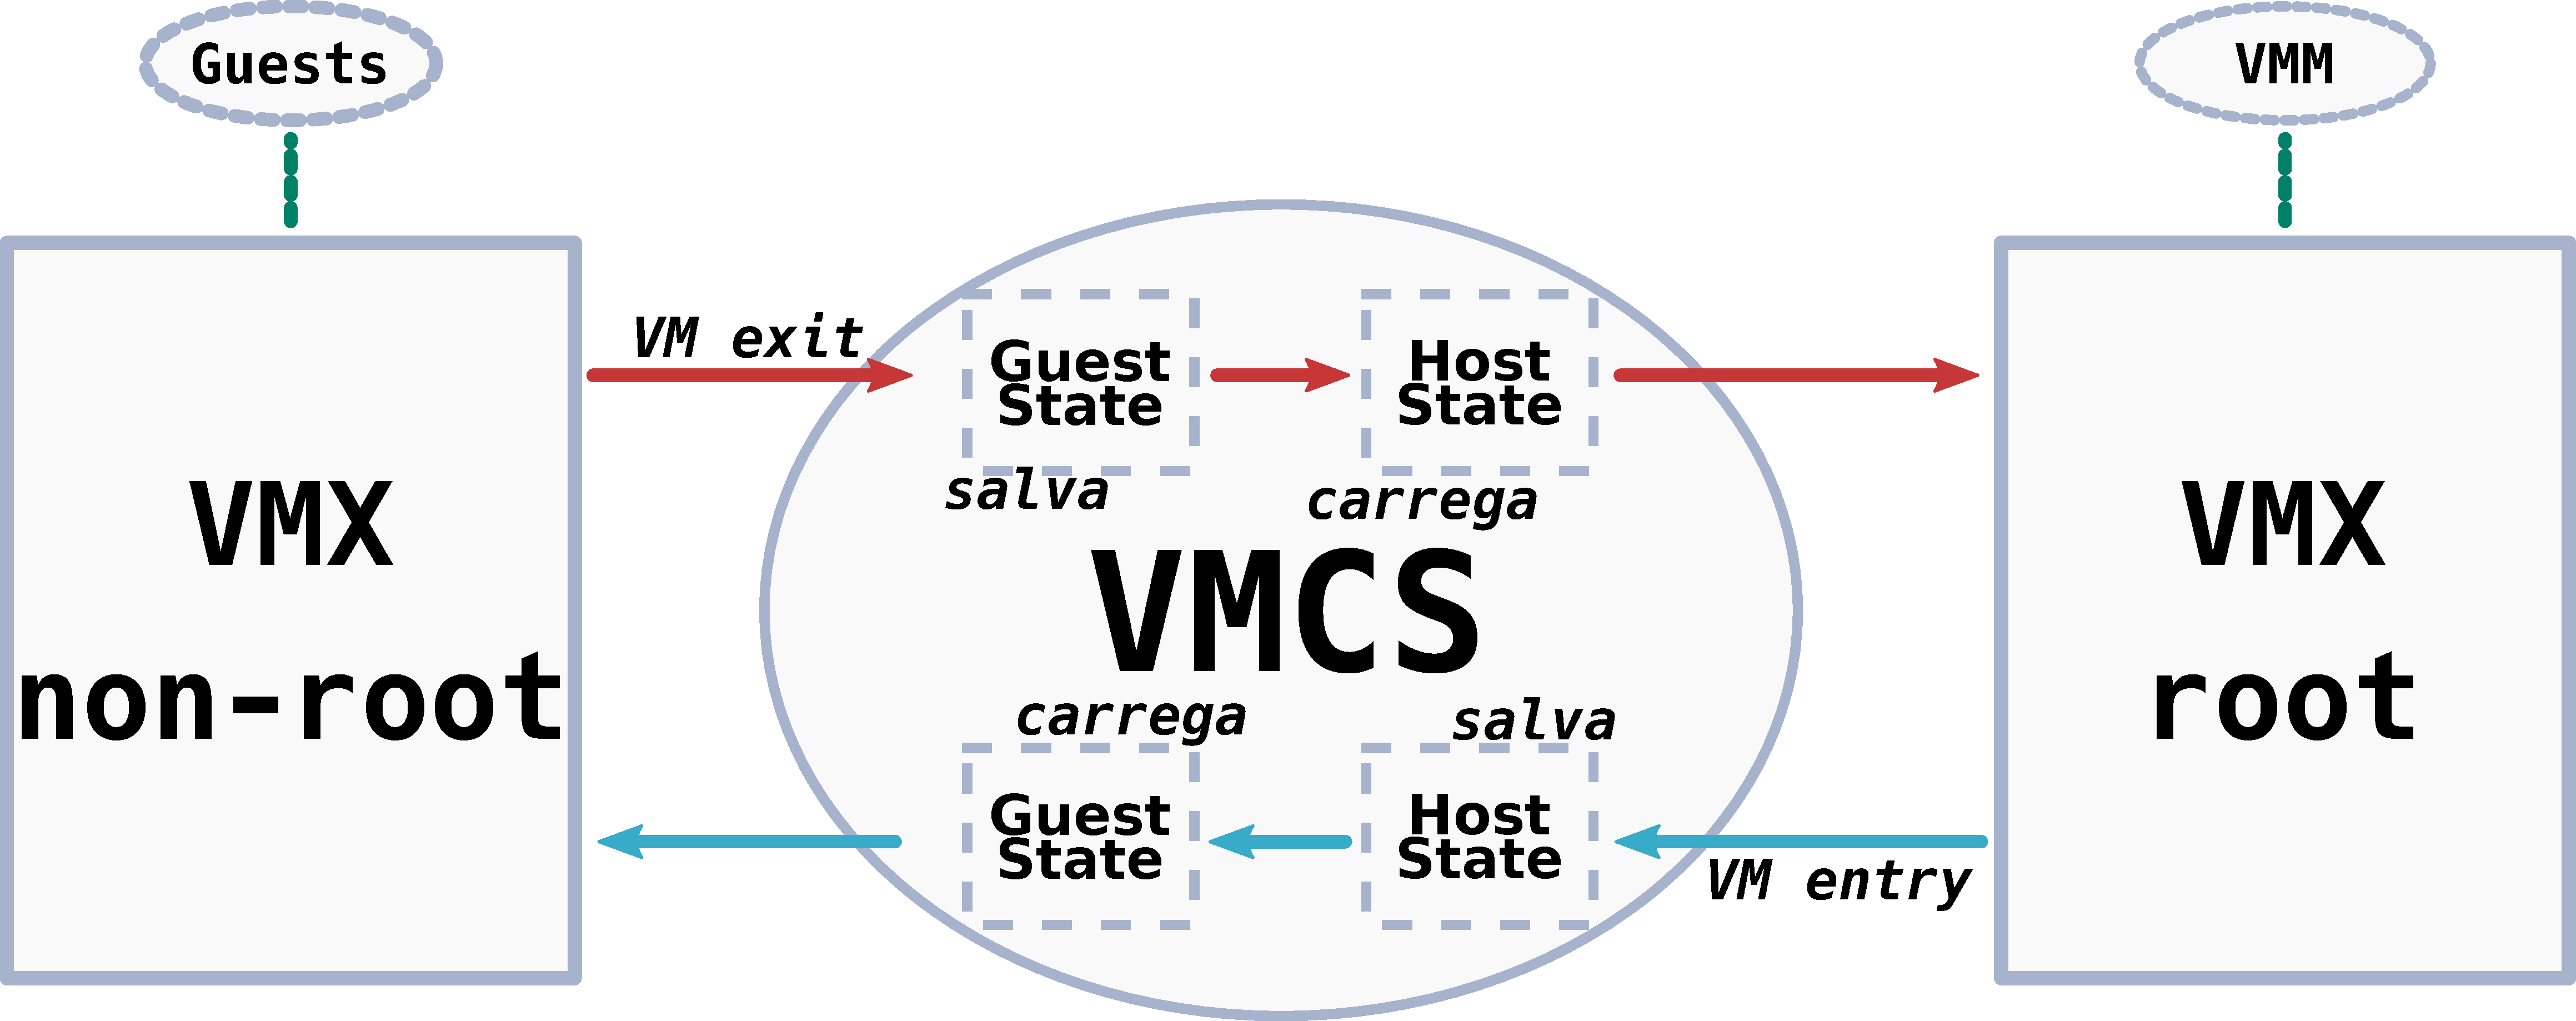
\includegraphics[width=0.6\textwidth]{vt-x_flow} 
  \caption{Fluxo do comportamento da tecnologia VT-x}
  \label{fig:vt-x_flow}
\end{figure}

O \emph{VMX non-root} é o modo de operação na qual a máquina \emph{guest}
executa, enquanto o \emph{VMX root} é o modo de operação utilizado pelo VMM. É
interessante observar que os dois modos tem suporte para os quatro níveis de
privilégios fornecidos pelos processadores Intel, isto permite que a máquina
\emph{guest} que tente executar uma instrução privilégiada em algum desses
nível forneçam tal informação para o VMM. Contudo, os software executando como
\emph{VMX non-root} são desprivilegiados de certa forma, a não pelo nível de
privilégios. Note da Figura \ref{fig:vt-x_flow} que existe uma transição chamada
\emph{VM exit} e \emph{VM entry}. A transição \emph{VM exit} ocorre quando o
controle é transferido do \emph{guest} para o VMM, isto faz com que o estado da
máquina \emph{guest} seja salvo e o estado do \emph{host} seja carregado para
que o VMM decida como tratar a interrupção. No sentido oposto, ocorre a
transição \emph{VM entry} na qual o VMM transfere o controle para a máquina
\emph{guest}, para isto ela salva o estado do \emph{host} e carrega o estado
anterior do \emph{guest}. Todas as informações referentes a virtualização são
mantidas em uma estrutura de dados chamadas de \emph{virtual-machine control
structure (VMCS)} que basicamente tem por função gerenciar as transições entre
a \emph{VM entry} e \emph{VM exit}.


\par

\chapter{Trabalhos Analisados}
\label{cap:trabalhos-analisados}

Esse capítulo tem como objetivo destacar as principais pesquisas recentemente
realizadas com o objetivo de expandir as abstrações de processos. Para a
seleção dos trabalhos aqui apresentados, o autor levou em consideração os
seguintes aspectos: quantidade de citações dos trabalhos, implementação
funcional e pesquisas que tenham a abstração de processos como objeto de
estudo. Por uma questão de organização, esse trabalho considerou três tipos de
implementação funcional: \textit{Implementação Estrutural Leve, Implementação
Estrutural Pesada e Implementação Independente}.

Chamamos de \boldAndIndex{Implementação estrutural leve} toda proposta que não
altera diretamente o núcleo do SO. Isso faz com que a proposta tenha uma chance
maior de ser incorporada em um SO de produção e, ao mesmo tempo, gera pouco
impacto geral no SO. Normalmente, implementações leves utilizam artifícios de
\emph{device drivers} (Veja \ref{sec:dd}), o que torna simples de desenvolver e
testar novas propostas.

As \boldAndIndex{Implementações Estruturais Pesadas} são aquelas que alteram
diretamente o núcleo do SO. Essa abordagem traz vantagens e desvantagens que
devem ser consideradas antes de serem adotadas. Por um lado, alterações diretas
no núcleo são mais flexíveis em termos de possibilidade de acesso aos recursos
disponíveis do SO. Por outro lado, alterações no núcleo são arriscadas, uma vez
que podem afetar toda a estabilidade do sistema, e são extremamente complexas
de serem feitas, uma vez que demandam profundo conhecimento do SO em questão.

As \boldAndIndex{Implementações Independentes} são aquelas que se propõem a
criar um SO totalmente novo, visando demonstrar um ou mais conceitos. Essas
abordagens têm poucas chances de serem adotadas diretamente, contudo apresentam
conceitos e ideias que podem ser interessantes para serem estendidas para SOs
atuais. Nessa dissertação trataremos especificamente do Exokernel devido ao seu
grande impacto (Seção~\ref{sec:exokernel}), contudo, trabalhos como o
\emph{Singularity}~\citep{aiken} e o \emph{Corey}~\citep{corey} também
influenciaram essa dissertação.

Em resumo, esse capítulo busca fornecer uma visão geral sobre o estado da arte
das abstrações de processos. Além disto, essa seção visa proporciona as bases
para a discussão apresentada no Capítulo
\ref{cap:analise-sobre-abstracoes-de-processos}, tema central desse trabalho.
Os trabalhos apresentados adiante, se encaixam em pelo menos uma das
características de implementação discutidas acima.

\section{Dune}
\label{sec:dune}

Como mostrado na Seção \ref{sec:virtualizacao}, o conceito de virtualização já
é amplamente conhecido e adotado pela indústria; dentre os recentes avanços,
destaca-se a virtualização via hardware proporcionada pelos processadores
modernos. O mecanismo de virtualização é normalmente utilizado fornecendo
abstrações para a criação de máquinas virtuais. Com esse conceito em mente,
\citet{belay} decidiram dar outra utilidade para esses recursos de hardware:
fornecer características adicionais para processos ao invés de máquinas
virtuais.

Os autores defendem que uma ampla variedade de aplicações pode tirar proveito
do acesso a certos recursos que são apenas disponíveis ao kernel. Dentre as
aplicações que podem comprovadamente ganhar algum desempenho ao obter acesso
direto ao hardware, destacam-se:

\begin{itemize}
  \item \textbf{Coletor de Lixo (\emph{Garbage Collection -- GC})}: O GC pode ganhar desempenho caso
        tenha como controlar diretamente o hardware de paginação, como
        \citet{pauseless} demostraram em seu trabalho;
  \item \textbf{Migração de Processos}: Programas no espaço de usuário podem tirar
        proveito do acesso direto às faltas de páginas e chamadas de sistemas para
        implementar novas técnicas de migração de processos.
\end{itemize}

Não obstante, fornecer o acesso direto aos recursos de hardware de forma segura
e gerenciável não é uma tarefa trivial, uma vez que requer mudanças na forma
como o espaço de usuário e o espaço do Kernel interagem. Além disso, alterações
no Kernel são consideradas invasivas e perigosas, uma vez que uma modificação
feita de forma errada pode comprometer toda a estabilidade do sistema. Outra
alternativa para dar acesso de hardware para aplicações é por meio de execução
em uma máquina virtual assim uma aplicação consegue acesso seguro aos recursos
de hardware através da interface de virtualização. Uma desvantagem desta
abordagem é que ela tem pouca integração com o SO da máquina \emph{host}, o que
impede o processo de obter ganhos de desempenho.

\citet{belay} oferecem uma alternativa que consiste em utilizar a abstração de
virtualização disponível nos processadores modernos de forma a fornecer um novo
tipo de processo que executa no chamado \emph{Dune Mode} (modo Dune). Tal modo
é um estado irreversível no qual o processo indica explicitamente que quer
entrar; nesse modo, o processo passa a ter acesso direto, por meio dos recursos
de virtualização, a modos de operação com maior privilégio, registradores de
memória virtual, tabelas de páginas, interrupções, exceções e vetores de
chamada de sistema. Para auxiliar a aplicação no espaço de usuário a interagir
com tais recursos, os autores criaram uma biblioteca chamada \emph{libDune} que
dá apoio à utilização das novas funcionalidades.

Dentre as vantagens que essa pesquisa promete, destacam-se o fato de que o modo
Dune mantém a compatibilidade com os processos, i.e., a aplicação não precisa
ser fortemente modificada. Quando um processo faz uma chamada de sistema, ele
dispara uma instrução chamada \texttt{SYSCALL}, contudo, aplicações que
manipulam recursos de virtualização utilizam a \texttt{VMCALL} para manter o
isolamento. O Dune utiliza o recurso do \texttt{VMCALL} para tirar o máximo
de isolamento fornecido pelo hardware de virtualização. Além disso, devido ao
fato de que o Dune não tem por objetivo fornecer máquinas virtuais, ele
consegue ser mais simples e rápido. As aplicações que se adequam ao uso desse
modelo podem obter melhorias de desempenho e isolamento, como veremos adiante.

Para implementar o Dune, os pesquisadores utilizaram processadores Intel com
suporte para a tecnologia VT-x e parte do código do KVM já disponível no Kernel
Linux. Na Seção~\ref{sec:vtx} apresentamos o VT-x e algumas instruções
importantes para o contexto da virtualização, agora introduzimos os três tipos
de instruções privilegiadas que o Dune fornece para os processos:

\begin{itemize}
	\item \textbf{Exceções}:  As instruções \texttt{LIDT, LTR, IRET, STI e CLI} são
        expostas diretamente para os processos. Note que emulação, depuração e
        rastreamento de desempenho são atividades que podem tirar proveito
        desta característica, uma vez que o Dune pode reduzir consideravelmente
        a sobrecarga em entregar exceções. Isso se deve ao fato que o Dune
        consegue entregar exceções diretamente para o hardware de forma segura
        (encapsulado pelo hardware de virtualização);
  \item \textbf{Memória Virtual}: As instruções \texttt{MOV CRn, INVLPG} e
        \texttt{INVPCID} são oferecidas para o processo Dune. O acesso
        flexível à memória virtual pode ser benéfico para aplicações que fazem
        \emph{checkpointing}, GC, compressão de dados nas páginas e utilizam memória
        compartilhada distribuída. O Dune traz melhorias para o acesso à
        memória virtual expondo as entradas da tabela de páginas para as
        aplicações. Isso permite que elas controlem a tradução de endereços,
        as permissões de acesso, bits globais e que elas modifiquem/acessem as páginas com
        simples referências. Por fim, o Dune também dá a habilidade de
        controlar as invalidações da TLB manualmente, o que pode ser vantajoso
        para alguns tipos de aplicações;
  \item \textbf{Modos privilegiados}: As instruções \texttt{SYSRET, SYSEXIT, IRET}
        permitem que o Dune exponha os modos privilegiados de
        forma segura. O Dune expõe esse modos de forma eficiente e segura por
        que o VMX non-root mantém o seu próprio conjunto de anéis privilegiados
        (Veja \ref{sec:vtx}).
\end{itemize}

A Figura \ref{fig:dune_architecture} ilustra a arquitetura do Dune. O Dune
estende o Kernel como um módulo que habilita o VT-x, colocando-o no
modo VMX root. Assim, processos usando Dune têm acesso seguro e garantido para
hardware privilegiado utilizando o modo VMX non-root. O módulo Dune intercepta
transições para o {VM exits} (Seção~\ref{sec:vtx}), o único motivo para o
processo acessar o kernel e realizar qualquer ação. Repare que o Dune é
aplicado de forma seletiva aos processos que de fato precisam dele, o que
significa que um processo que não usa o Dune não é afetado. A transição de um
processo normal para o modo Dune ocorre por meio de uma chamada de
\texttt{ioctl} no dispositivo \texttt{/dev/dune} e, ao entrar nesse modo, o
processo não pode retornar ao modo anterior. Sempre que um processo Dune faz um
\texttt{fork()}, o processo filho não inicia em modo Dune, contudo pode
reentrar caso queira.

\begin{figure}[!h]
  \centering
  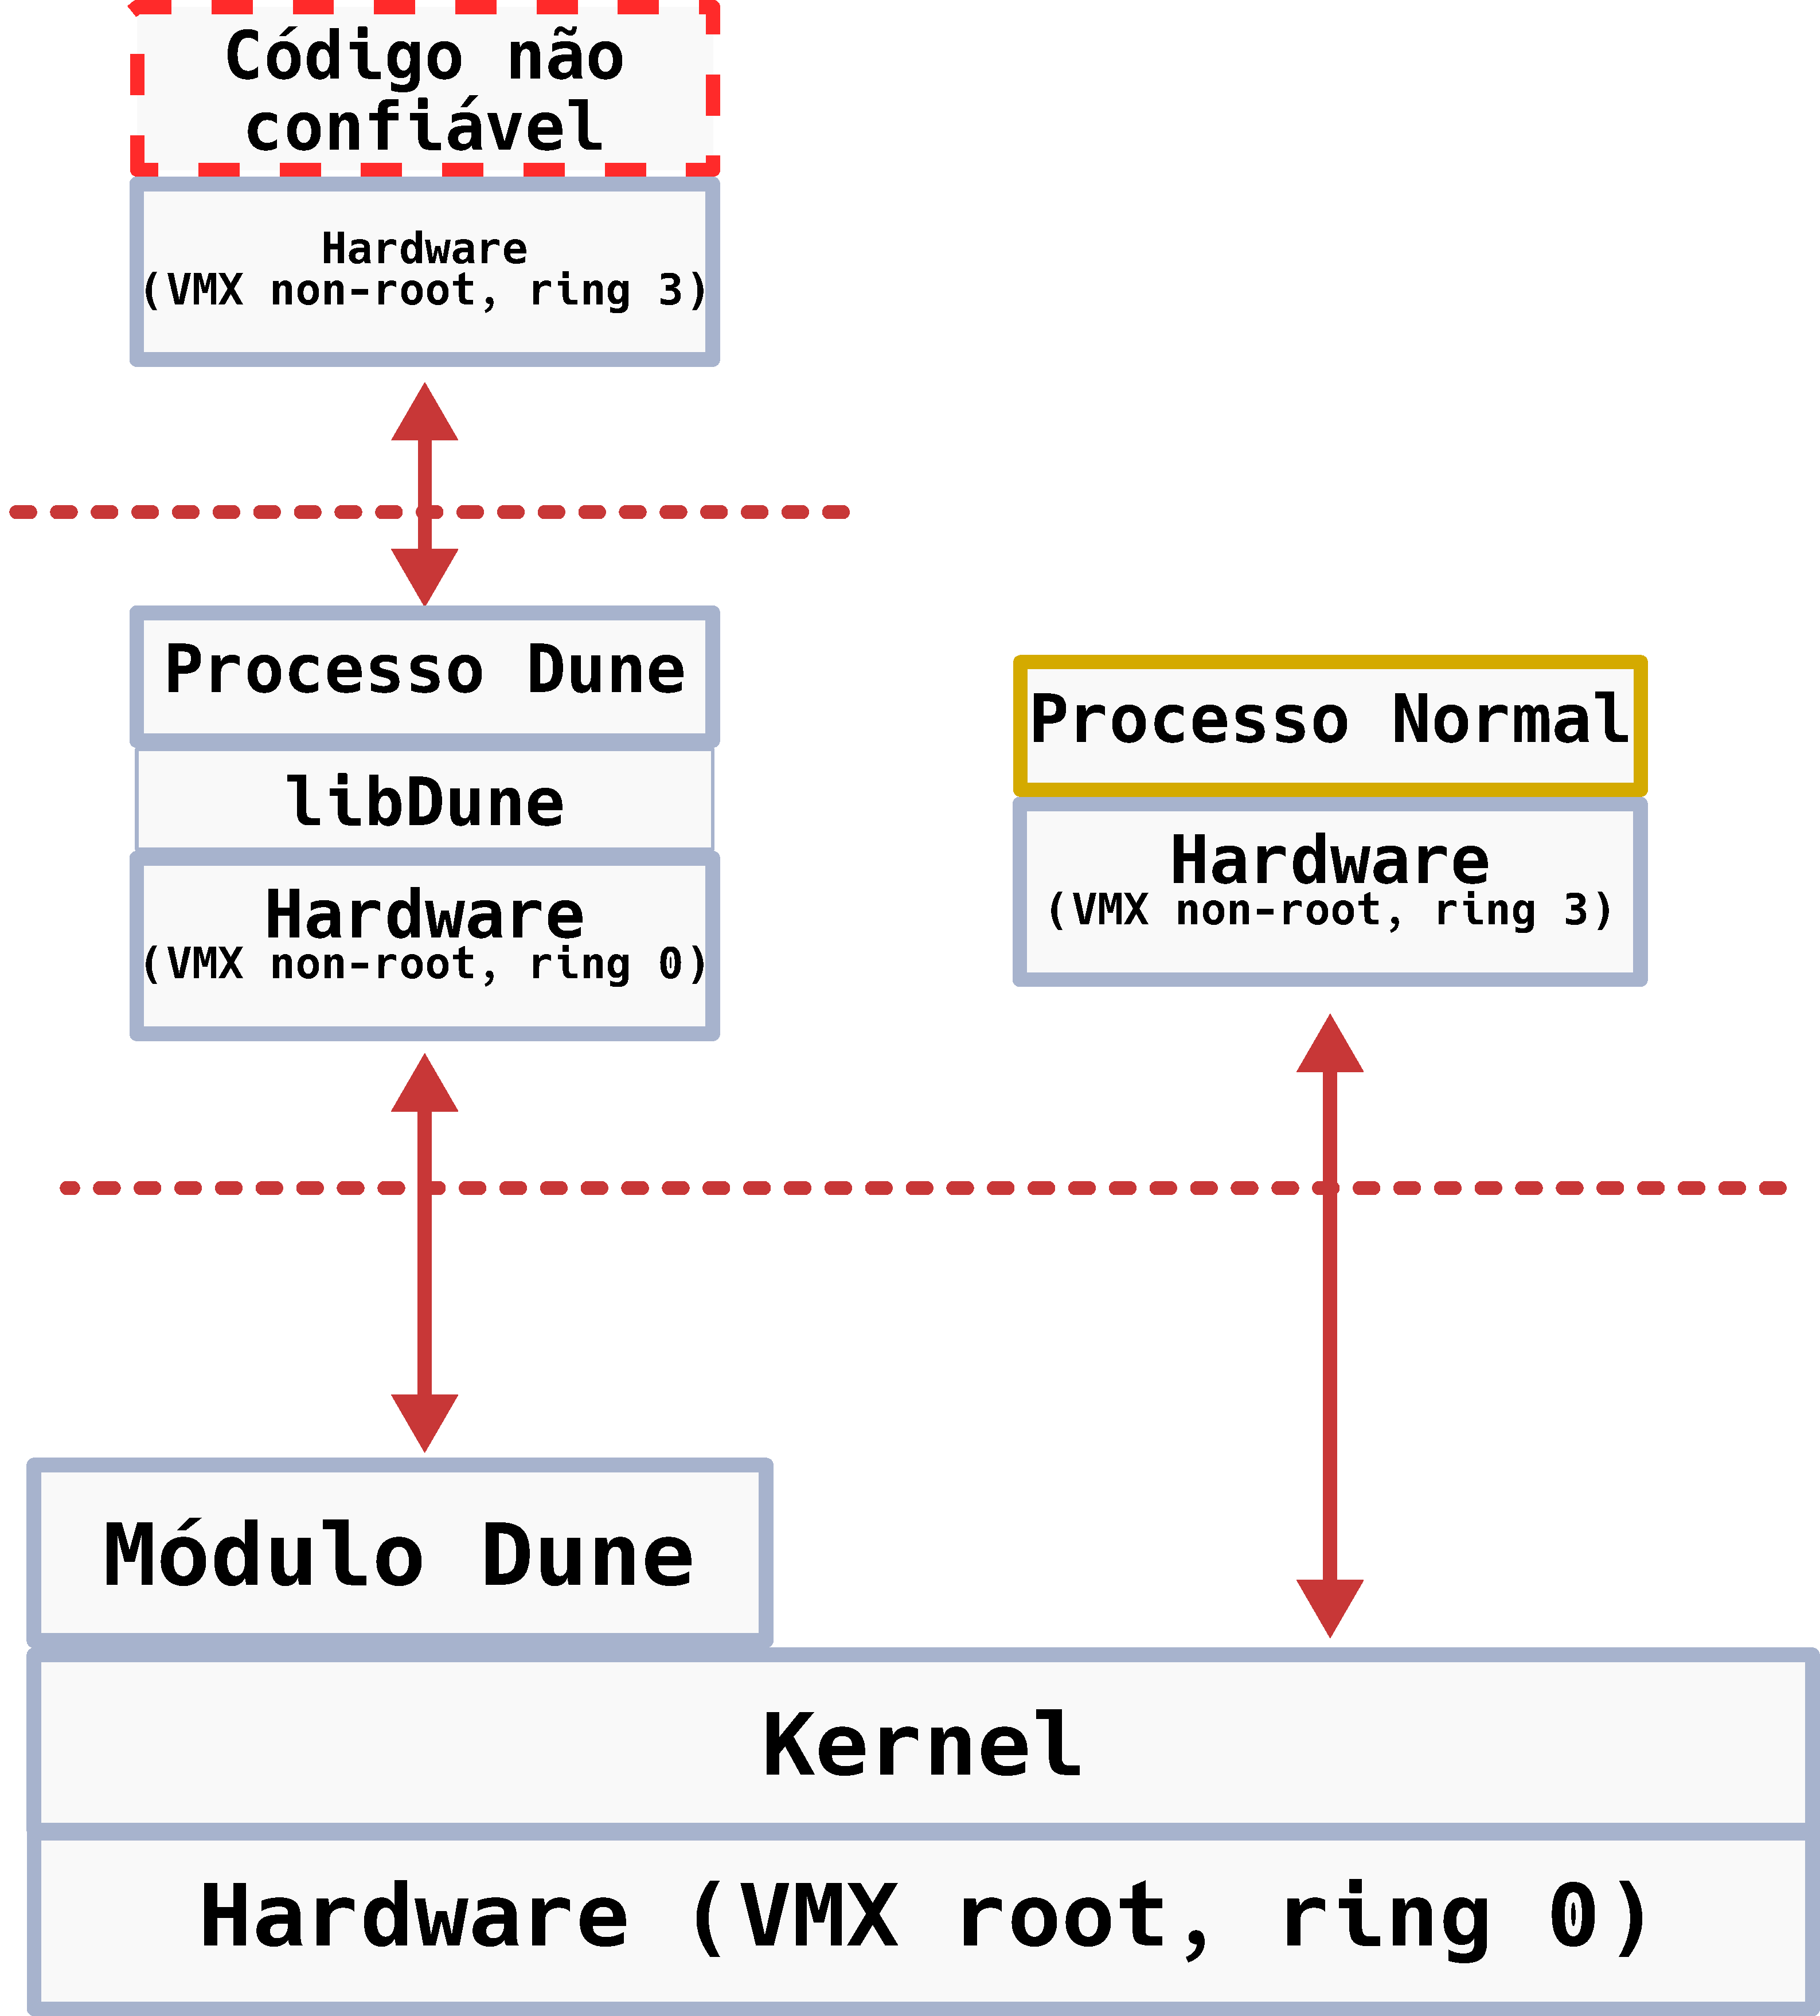
\includegraphics[width=0.6\textwidth]{dune_architecture} 
	\caption[Arquitetura do Dune]{Arquitetura do Dune~\citep{belay}}
  \label{fig:dune_architecture}
\end{figure}

Na Seção \ref{sec:virtualizacao}, apresentamos as principais propriedades dos VMMs.
Com o objetivo de deixar claras as diferenças entre o VMM e as características
de hardware expostas pelo Dune, destacamos as principais diferenças:

\begin{itemize}
  \item No Dune, o mecanismo de \textit{hypercall} invoca
        \textit{system calls} comuns do Linux;
  \item Apenas características de hardware que podem ser acessadas diretamente,
        sem a intervenção do VMM, são disponíveis para a aplicação. Nos casos em
        que não é possível executar uma dada operação, Dune devolve o controle
        para o SO;
  \item Podemos reduzir as diferenças de estados entre o \textit{guest} e o \textit{host}, uma
        vez que processos usando Dune têm uma interface próxima da de hardware;
  \item No Dune, é preciso configurar o EPT para refletir o endereço do espaço
        de usuário.
\end{itemize}

\section{Shreds}

Existe uma categoria de ataques chamada ``abusos intra-processos de conteúdo
de memória'', na qual o invasor busca acessar determinado tipo de conteúdo
sensível na memória (e.g., dados secretos) ou uma região de código crítica
(e.g., funções privilegiadas) \citep{shreds}. O roubo desse tipo de dados
acontece por meio da introdução de algum código injetado ou por meio de alguma
biblioteca maliciosa que permite acessar alguma região da memória não protegida
da vítima. Note que bibliotecas maliciosas são especialmente perigosas, uma vez
que elas podem executar funções privilegiadas que são de fato parte do
processo como, por exemplo, a função \texttt{dlopen}. Por fim, se o atacante
conseguir o acesso a memória, ele pode ler todos os dados buscando por outras
informações.

\citet{shreds} defendem que o problema de segurança referente aos ataques
intra-processos decorrem da falta de controle fino e eficiente do conteúdo
sensível da memória; além disso, eles argumentam que seria benéfico se tais
funcionalidades fossem disponibilizadas para os programadores. Para resolver tal
problema, os autores apresentam uma nova abstração de processos que cria uma
nova unidade de execução chamada \emph{shred}, que tem associado a si um
fragmento de memória protegida denominado \emph{shred-private pool
(s-pool)}. O tamanho do segmento de memória criado é variável,
dependendo da necessidade da aplicação. Além disso ele se comporta de forma a
existir apenas durante o momento em que é necessário para um pedaço da
aplicação. A implementação do \emph{shreds} é baseada em três pilares: uma API
para o usuário conseguir utilizar facilmente as funcionalidade oferecidas, um
conjunto de ferramentas de compilação que verifica a correta utilização dos
\emph{shreds} (\emph{S-compiler}) e um módulo Linux que faz o gerenciamento da
memória (\emph{S-driver}).

\emph{Shreds} foi projetado buscando três propriedades que visam garantir
segurança:

\begin{itemize}
  \item \textbf{Acesso exclusivo para s-pool:} Um \emph{s-pool} só é acessível
        para o \emph{shred} associado a ele;
  \item \textbf{controle de vazamentos na entrada e saída:} Dados carregados em um
        \emph{s-pool} não podem ser copiados ou exportado sem que seja
        executada uma operação de limpeza;
  \item \textbf{Execuções não desviáveis:} O fluxo de execução não pode ser
        alterado para fora do \emph{shred}.
\end{itemize}

Para melhor entender o comportamento dos \emph{shreds}, veja a Figura
\ref{fig:shreds}, ilustrando uma aplicação que lida com uma senha (dado
sensível) e o código que manipula tal dado. A aplicação possui uma \emph{thread} que
comporta-se da forma padrão, contudo, ao ter que lidar com um dado sensível, ela
faz uma chamada para uma função da API fornecida pelo \emph{shred},
\texttt{shred\_enter()}. Ao realizar a chamada para essa função, o fluxo de
execução entra em um modo seguro em que o \emph{shreds} gerencia o acesso à
memória e garante que os dados são isolados do restante da aplicação. Por fim,
após realizar a operação na região protegida, a aplicação do usuário chama
\texttt{shred\_exit()}. Para utilizar a proposta dos autores, é preciso alterar
as aplicações alvo.

\begin{figure}[!h]
  \centering
  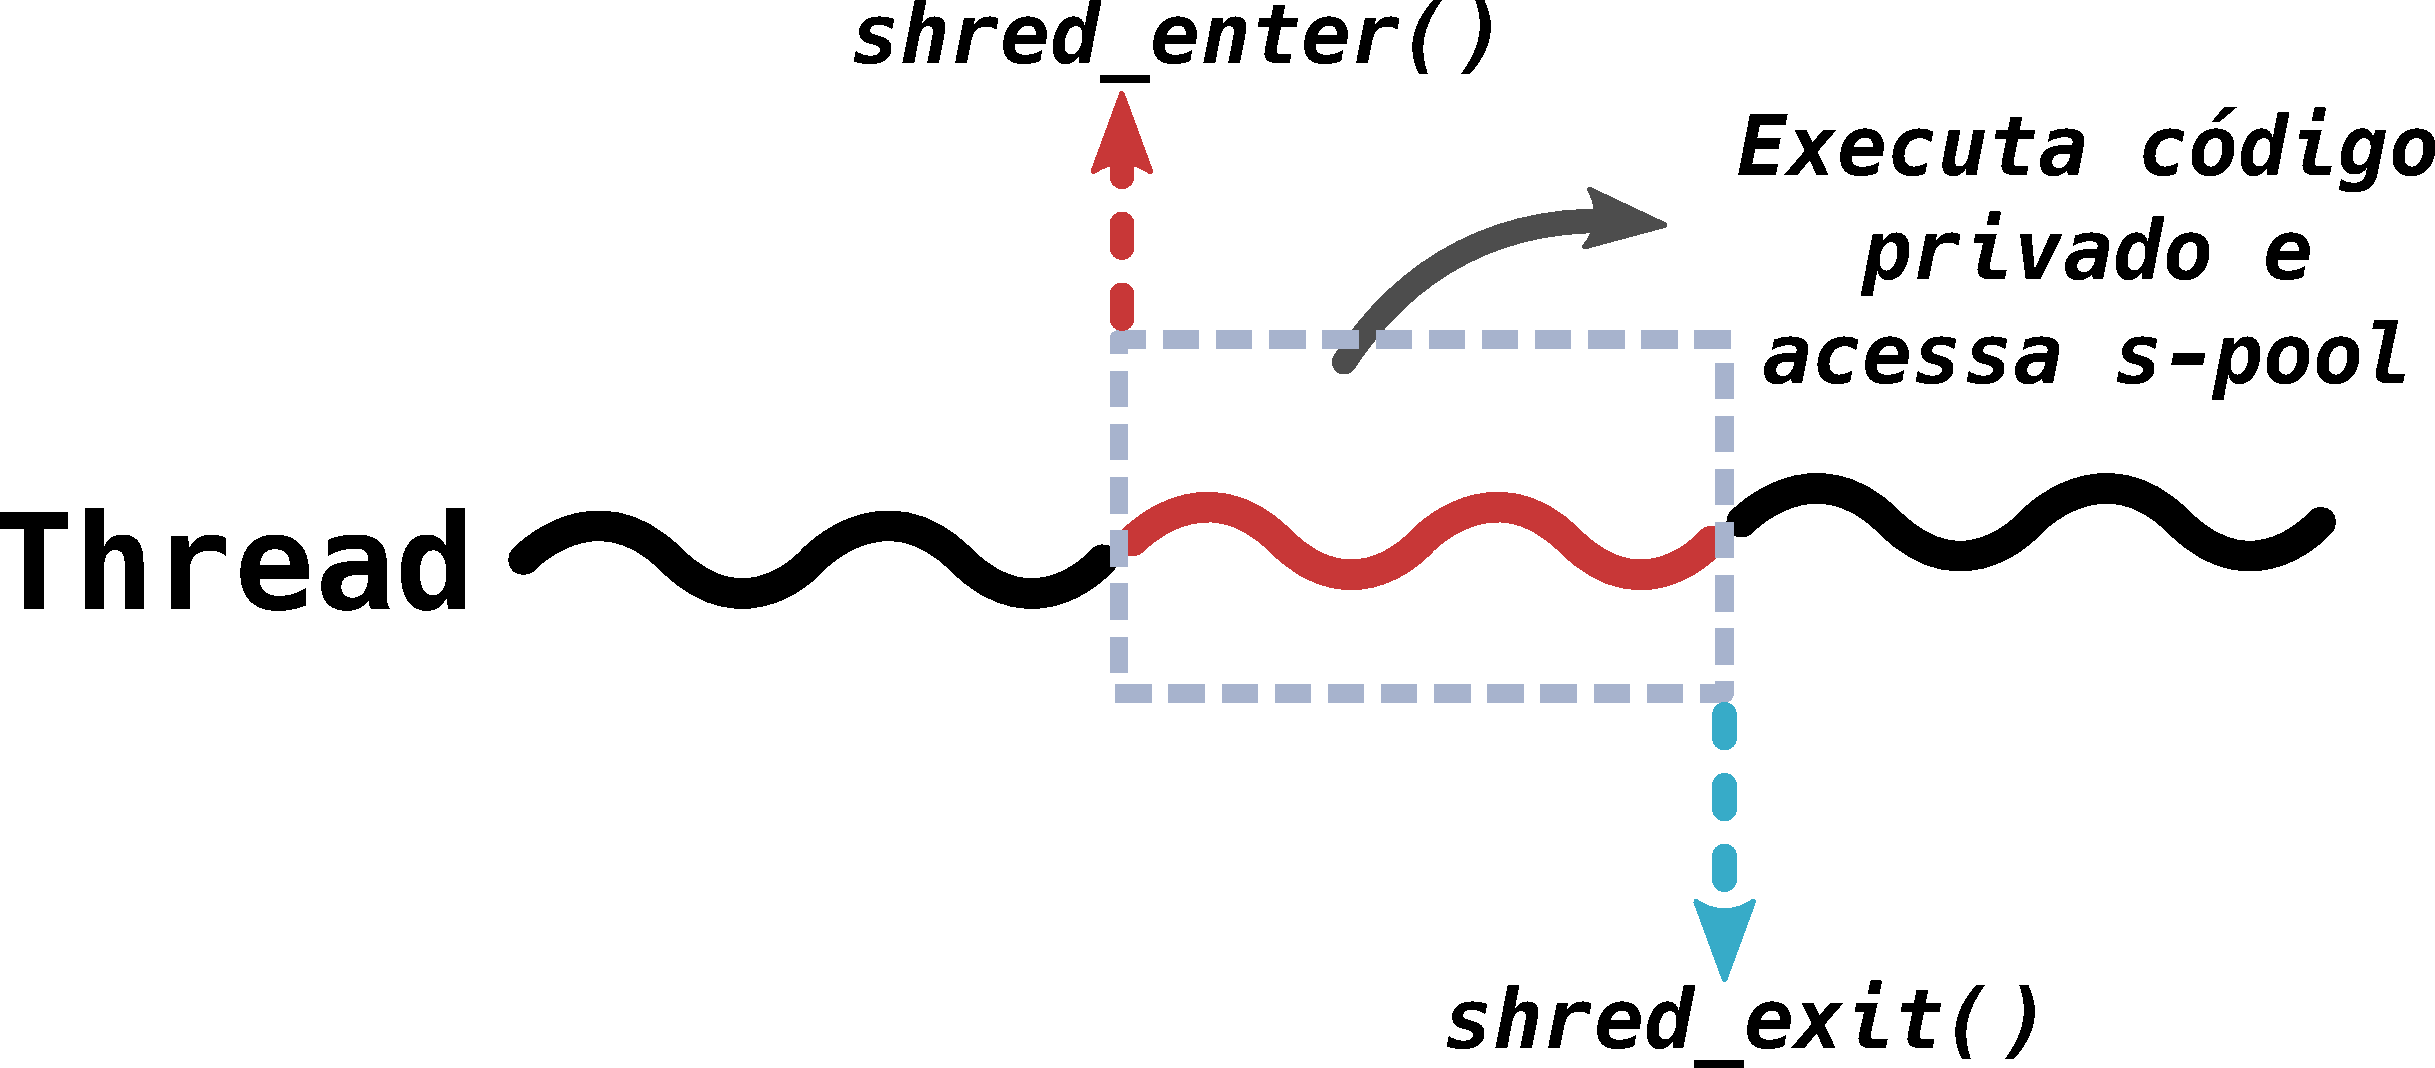
\includegraphics[width=0.6\textwidth]{shreds} 
  \caption{Funcionamento geral do shreds}
  \label{fig:shreds}
\end{figure}

A API fornecida pelo \emph{shreds} consiste em apenas quatro funções:

\begin{itemize}
  \item \texttt{shred\_enter()}: Muda o fluxo de execução da \emph{thread} atual e
        cria uma cópia da pilha atual do processo em uma região de memória
        segura (\emph{pool});
  \item \texttt{shred\_exit()}: Suspende o \emph{shred} chamado, revoga as permissões
        de acesso da \emph{thread} atual sobre o \textit{s-pool} e recupera a pilha de execução
        original;
  \item \texttt{spool\_alloc()}: Aloca memória para o \emph{s-pool} associado à
        \emph{thread};
  \item \texttt{spool\_free()}: Apaga a memória alocada.
\end{itemize}

Para garantir que as regras de utilização da API sejam seguidas, o
\emph{S-compiler} realiza verificações e instrumentações para evitar falhas que
abram brechas de segurança.

Para este trabalho, a parte mais importante do \emph{shred} é o \emph{S-driver},
que consiste em um módulo do Linux responsável por gerir os \emph{shreds} e
\emph{s-pools}. A implementação dessa técnica é baseada em domínios de memória
do ARM (Seção \ref{sec:outros_mecanismos_memoria}). Contudo, dado que essa
tecnologia não foi projetada para os propósitos sugeridos pelo \emph{shreds},
ela apresenta duas limitações:

\begin{itemize}
  \item O ARM fornece apenas 16 domínios, o que impede que se crie um domínio
        para cada \emph{s-pool}, uma vez que seu número pode crescer de forma
        indeterminada;
  \item O controle de acesso à memória é extremamente limitado.
\end{itemize}

A solução adotada pelos autores foi implementar um mecanismo que multiplexa os
domínios e introduz identidades dentro da lógica de acesso. Para permitir que
uma aplicação tenha várias \emph{shreds}, o \emph{S-driver} utiliza os domínios
de forma temporária, rotacionando as identidades de segurança para o
\emph{s-pool}. Toda vez que uma \emph{shreds} inicia ou retoma a sua execução
em uma $CPU_i$ o \emph{S-driver} atribui um \emph{s-pool} associado a um
domínio $Dom_i$. Isso faz com que uma \emph{shred} consiga acessar o seu
\emph{s-pool} enquanto outras \emph{threads} concorrentes não. Quando o
\emph{shred} finaliza ou tem a sua execução parada em favor de outro
processo, o \emph{S-driver} muda o domínio, prevenindo que outro processo
consiga acessar a região de memória. Note que o \emph{driver} permite ou
rejeita o acesso a um \emph{s-pool} baseado na CPU; isso faz com que, mesmo que
um código malicioso consiga executar em paralelo com o \emph{shred}, ele não
consiga ter acesso ao \emph{s-pool} sem que seja disparada uma falha de
domínio.

Uma das funcionalidades fornecidas pelo \emph{shread} é a habilidade de
permitir fazer cópias de dados para regiões de memória não protegidas de forma segura
(e.g., atribuir dados de um \emph{s-pool} para uma variável local). Note que,
para realizar tal procedimento, é preciso acessar uma stack regular que pode ter
sido atacada e conter um código mal-intencionado, o que violaria toda proteção
fornecida pelo \emph{s-compiler} e \emph{S-driver}. Para prevenir que dados
sejam vazados via stack, o \emph{S-driver} cria uma stack segura para cada
\emph{shred} alocada partindo do \emph{s-pool} associado a si.

\section{Wedge}

Existe um princípio chamado de \emph{``Princípio do Menor Privilégio''} que diz:

\begin{quote}
O princípio do menor privilégio implica dividir o código em compartimentos,
cada um dos quais executa com os privilégios mínimos necessários para completar
sua tarefa. Essa abordagem não apenas limita o dano que um ataque pode causar,
mas também pode evitar que os \emph{bugs} vazem acidentalmente informações
confidenciais.
\end{quote}

Apesar desse princípio ter sido apresentado em 1975 e ser amplamente aceito,
nota-se que várias aplicações que tem acesso à Internet (um ponto de acesso
para o mundo) não buscam atender a esse fundamento e acabam abrindo
potenciais pontes de vazamento de dados ou falhas de segurança. Alguns
pesquisadores defendem que esse problema surge do fato de que os SO atuais
garantem privilégios por padrão. Isso significa que impor limites requer mais
esforço por parte do programador e também é propenso a erros.

A chamada de sistema \texttt{fork()} ilustra a característica de garantir
privilégios por padrão. Quando o processo pai cria um filho, este inicia como uma
cópia praticamente exata do pai. Se o programador desejar restringir o nível de
acesso do processo filho, é preciso realizar uma série de operações manuais que
não garantem que nenhum aspecto tenha sido ignorado.

\citet{wedge} buscaram resolver tal problema mudando o princípio atual, de
garantir privilégio por padrão, para negar privilégios por padrão. Nessa
abordagem, o programador deve indicar explicitamente que deseja garantir
permissões adicionais. Os autores alteraram o GNU/Linux para que ele
suportasse a remoção de permissões por padrão e chamaram o modelo proposto por
eles de \emph{Wedge}. \emph{Wedge} fornece um conjunto de primitivas de
programação para permitir criar componentes com semântica de negação de permissões
por padrão, tornando o acesso mais restrito. Para isso, \emph{Wedge} oferece
um esquema simples e flexível de marcação (\emph{tagging}) das permissões de
acesso à memória, permitindo que o programador aloque objetos na memória de
acordo com essa informação.

\emph{Wedge} permite que o programador crie um número arbitrário de
componentes, cada um sem privilégios por padrão, mas existem mecanismos que
permitem o controle fino. Neste sentido, \emph{Wedge} busca se assemelhar às
primitivas atuais para facilitar a sua adoção e para que seja simples a
introdução delas em aplicações legadas. A proposta é constituída de três
primitivas: \emph{Sthread}, \emph{Tagged Memory} e \emph{callgates}. O
acesso a todas essas primitivas é feito via chamadas de sistema.

Uma \emph{Sthread} pode ser comparada com uma \emph{thread} fornecida pela biblioteca
\textit{pthread}, definindo um compartimento dentro de uma
aplicação. O programador pode então atribuir permissão de acesso para a memória
e outros recursos por meio dessas \emph{sthreads}. Elas consistem de uma
\emph{thread} de controle e políticas de segurança associadas, que especificam:

\begin{itemize}
	\item As marcações de memória que a \emph{sthread} pode acessar e a permissão
				sobre cada cada uma (leitura, leitura-escrita e \textit{copy-on-write});
	\item Os descritores de arquivo que a \emph{sthread} pode acessar e as
				permissões sobre cada (leitura, escrita, leitura-escrita);
	\item Os \emph{callgates} que a \emph{sthread} pode chamar;
	\item O \emph{Unix user id}, o diretório raiz, e o contexto SELinux.
\end{itemize}

Normalmente, quando uma cópia da memória é feita o SO apenas realiza a
duplicação quando o recurso é modificado (\emph{copy-on-write}); nesse contexto
uma nova \emph{sthread} não mantém as permissões de acesso por padrão, a não
ser pela memória ainda intocado do \emph{copy-on-write}. Note que o novo
componente não tem permissão para acessar qualquer outra memória ou mesmo
descritor de arquivo do pai, contudo o pai pode anexar permissões de acesso no
filho durante a sua criação. Uma \emph{sthread} só pode criar um filho com
permissão igual ou menor do que a sua. Para a implementação, os autores criaram
\emph{sthreads} como uma variante dos processos do GNU/Linux, só que, ao invés
de herdar as informações do pai, ela apenas herda as regiões de memória e
tabela de descritores asseguradas pela política de segurança.

No \emph{Wedge} é preciso seguir alguns passos para alocar memória. O passo
inicial consiste em criar uma \emph{tag} que contém as permissões de acesso a
região de memória que se deseja alocar. Em seguida, o programador deve utilizar
uma chamada específica do \emph{Wedge} para fazer a alocação, essa função
espera uma \emph{tag} que contém as permissões. Quando alguma alocação de
memória ocorre, o programador deve marcar a memória com uma única \emph{tag};
as permissões de acesso a esta memória são garantidas em termos delas. Essa
operação aloca um segmento de memória e armazena um mapa da \emph{tag} para o
segmento. Por exemplo, o programador pode criar uma \emph{tag} ``t'' que define
que a memória será apenas para leitura. O programador expressa os privilégios
de memória em termos das \emph{tags} que são atribuídas para a memória em tempo
de alocação.

Um \emph{callgate} é uma porção de código que executa em um nível de privilégio
(normalmente) diferente de quem o chamou. Como um \emph{sthread} sempre roda
com o menor privilégio possível, sempre que for preciso executar algo em um
nível de permissão maior, será preciso chamar um \emph{callgate} para executar
a operação. Para criar e usar um \emph{callgate}, é necessário indicar um ponto
de entrada, um conjunto de permissões e argumentos confiáveis fornecido pelo
responsável em criar o \emph{callgate}. \emph{Wedge} garante que os
argumentos passados e criados não podem ser adulterados pelo processo que o
utilizará. Além disso o \emph{callgate} herda o sistema de arquivos raiz e o id
do usuário que o criou. As permissões do \emph{callgate} precisam ser um
subconjunto de quem o criou. Depois que um \emph{callgate} foi criado, a
\emph{sthread} privilegiada pode criar um filho com menos privilégios mas com
acesso ao \emph{callgate} criado. Quando o filho tenta acessar o
\emph{callgate}, uma nova \emph{sthread} é criada e a execução é levada para o ponto
de entrada que foi registrado.

Para a implementação dos \emph{callgates}, a função \texttt{sc\_cgate\_add()}
adiciona permissões para o ponto de entrada \texttt{cgate} com as permissões e
os argumentos confiáveis, e todos esses dados são salvos no Kernel para evitar
acessos indevidos. Um \emph{callgate} é invocado por meio da função
\texttt{cgate()}, que faz com que o Kernel verifique as permissões. De forma
geral, a API do \emph{Wedge} é composta por diversas funções; destacamos apenas
algumas:

\begin{itemize}
  \item \texttt{sthread\_create(sthread\_t, sc\_t, cb\_t, void *arg)}: Cria
uma nova \emph{sthread};
  \item \texttt{tag\_t tag\_new()}: Cria uma nova \emph{tag};
  \item \texttt{tag\_delete(tag\_t)}: Remove uma \emph{tag};
  \item \texttt{smalloc(int sz, tag\_t tag)}: Aloca memória baseada na
informação de tamanho e na \emph{tag};
  \item \texttt{sfree(void *x)}: Libera a memória previamente alocada com o
\texttt{smalloc()}
  \item \texttt{sc\_cgate\_add(sc\_t sc, cg\_t cgate, sc\_t *cgsc, void *arg)}:
Adiciona permissões para chamar um \emph{callgate};
  \item \texttt{cgate(cg\_t cb, sc\_t *perms, void *args)}: Invoca um
\emph{callgate}.
\end{itemize}

\section{Resource Container}
\label{sec:rc}

\citet{resourcecontainers} argumentam que as abstrações de SO têm recebido
grandes contribuições para melhorar questões de desempenho, mas que
pouca atenção tem sido dada para o gerenciamento de recursos. Como exemplo, os
autores mostram como a gerência de recursos é um elemento crítico para conter
ataques como o \emph{Denial-of-Service Attack}, que basicamente consiste em fazer
com que todos os recursos da máquina sejam consumidos. Eles também
assumem que a raiz dos problemas de gestão de
recursos encontra-se no modelo atual dos SOs de propósito geral, em
que primitivas de escalonamento e de gerência de recursos estendem-se por todo
o Kernel. Esse acoplamento torna complicado o processo de permitir que uma
aplicação controle os seus próprios recursos.

\begin{figure}[!h]
  \centering
  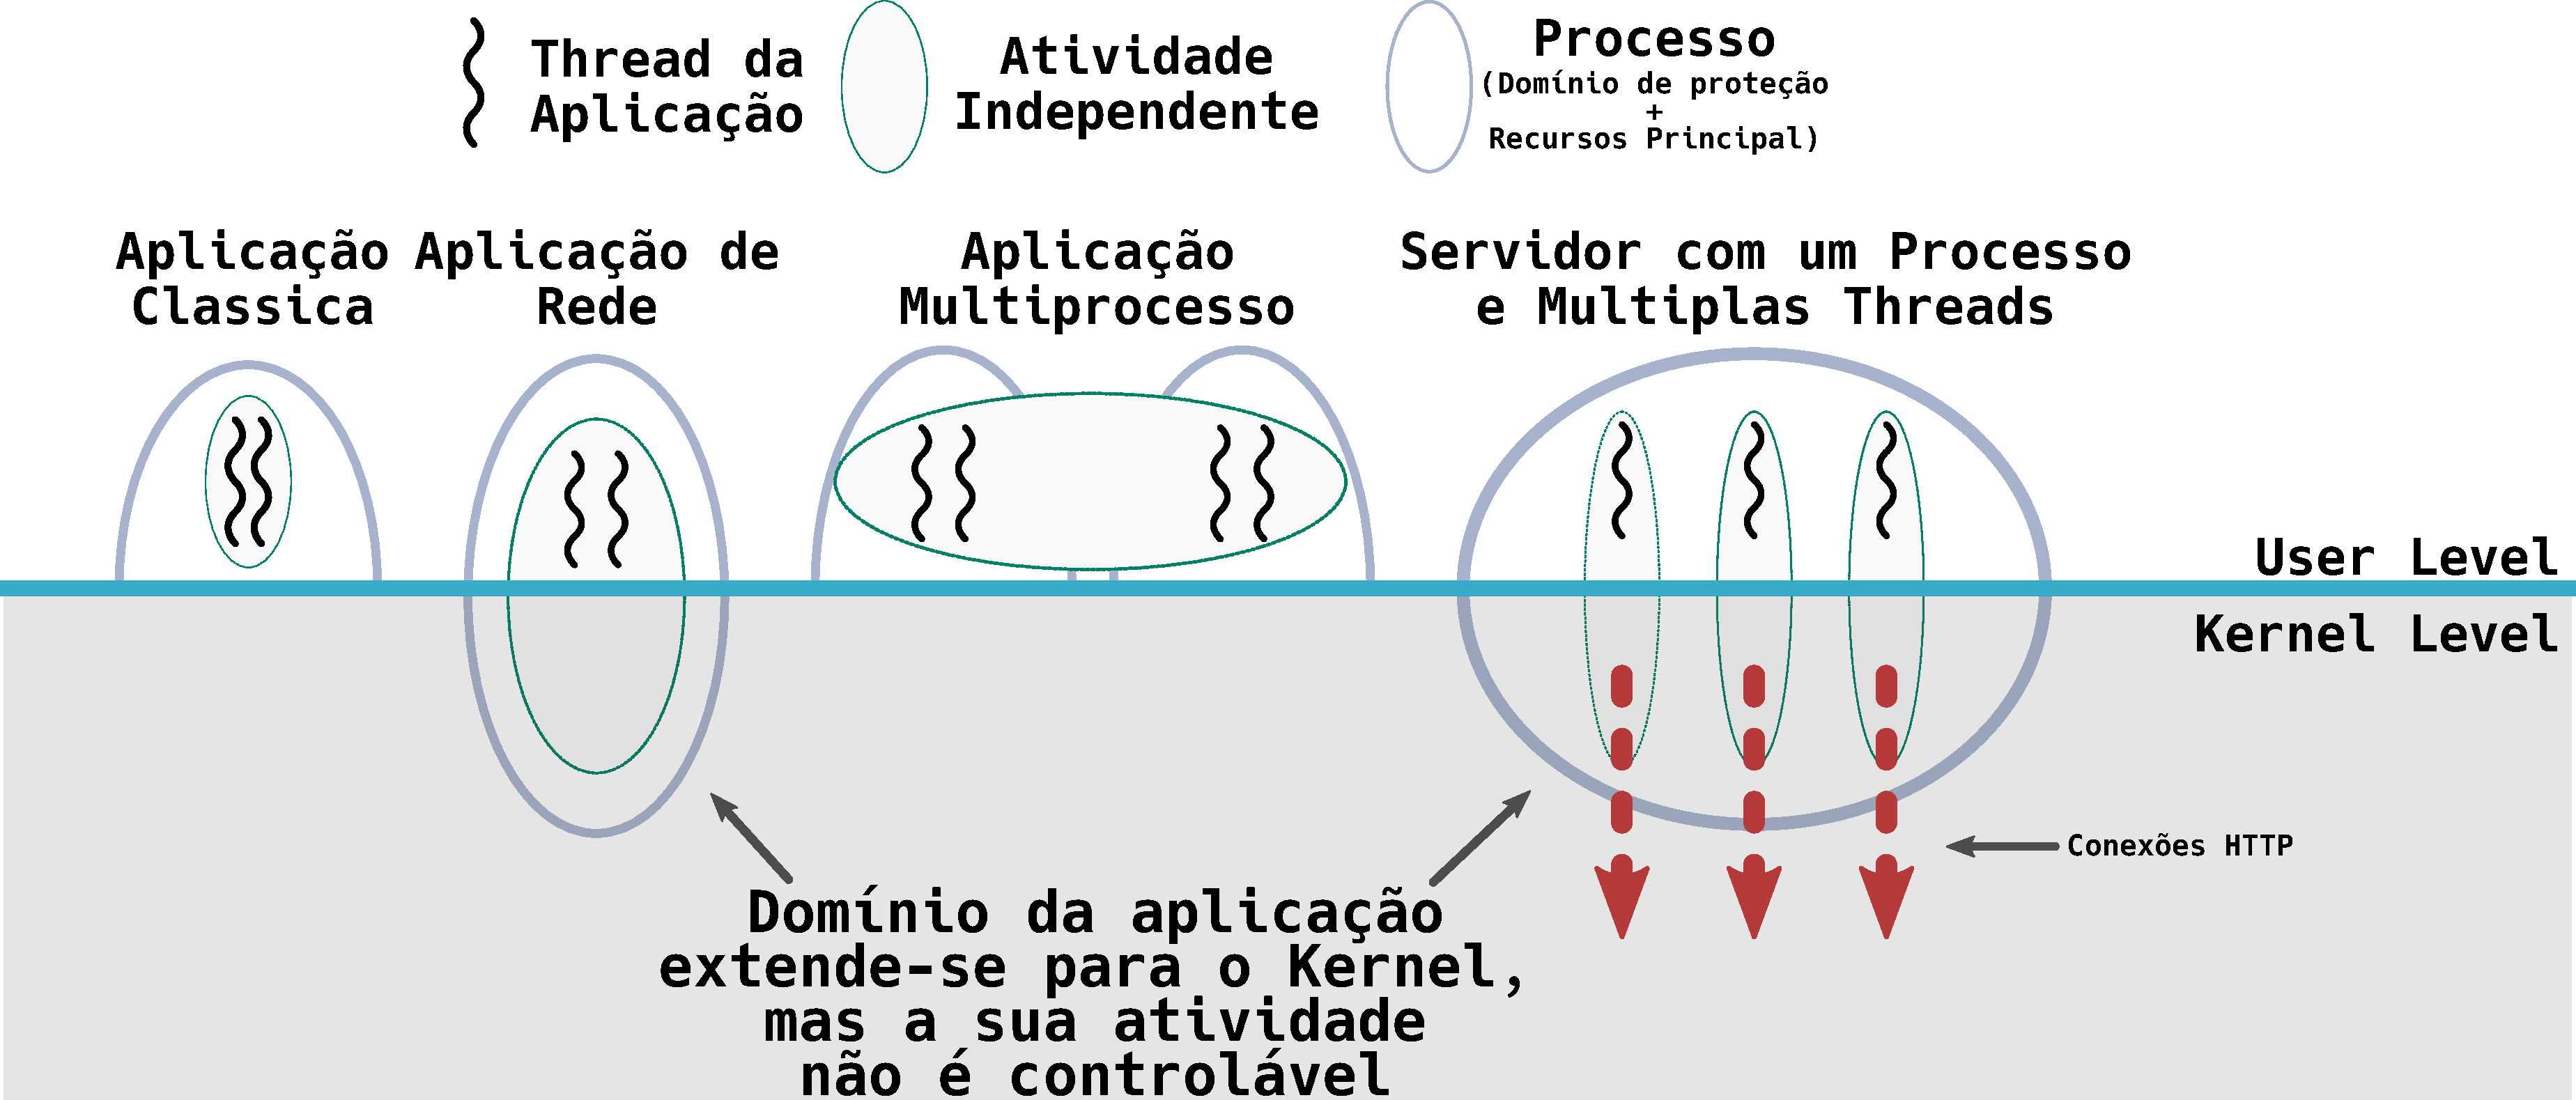
\includegraphics[width=\textwidth]{resource_constainer_scenarios} 
  \caption{Cenários das aplicações}
  \label{fig:resource_constainer_scenarios}
\end{figure}

Para ilustrar as questões referentes à gestão de recursos nos SOs, a Figura
\ref{fig:resource_constainer_scenarios} mostra 4 cenários diferentes. O
primeiro cenário consiste em uma aplicação rodando em \textit{user space} que
não necessita de qualquer recurso diretamente controlado pelo Kernel e,
portanto, cujo consumo de recursos não se estende para o Kernel. O segundo
cenário representa uma aplicação que precisa utilizar recursos do Kernel para
terminar alguma de suas tarefas (e.g., um software que usa recursos de rede).
Note que parte da aplicação consome recursos dentro do \textit{user space};
contudo, a outra parte da aplicação se expande para o Kernel. O terceiro cenário
mostra múltiplos processos cooperando para concluir uma tarefa sem precisar
do Kernel. Por fim, temos uma aplicação com um único processo que dispõe de
múltiplas \emph{threads} que, além de utilizar recursos no \textit{user space}, também
demanda recursos oriundos do Kernel. Repare como sistemas tradicionais têm
pouco ou nenhum controle sobre os recursos consumidos;esses casos
podem levar o escalonador a fazer contagens imprecisas levando-o a
comportar-se de forma inadequada.

Inspirados pela falta de uma separação clara do gerenciamento de recursos por
parte dos SOs, \citet{resourcecontainers} sugeriram a criação de uma nova
abstração chamada \emph{Resource Container (RC)}. Este é uma entidade que
logicamente contém todos os recursos utilizados pela aplicação para completar
uma determinada atividade. Seus atributos são usados para fornecer parâmetros
de escalonamento, limites de recursos, e \emph{QoS} para rede. A ideia é que o
Kernel cuidadosamente manipule esses recursos, tal qual CPU e memória, consumidos
por um RC. O escalonador pode acessar as informações provenientes dos RCs e
utilizá-las para melhorar o processo de escalonamento.

A adição do RC cria uma clara distinção entre o domínio da proteção e o de
recursos, além de fornecer um controle fino sobre os recursos. O RC fornece um
mecanismo para ligar os recursos a uma \emph{thread}, de forma
dinâmica e sob controle da aplicação (isso também é chamado de \emph{resource
binding}). Note que isso permite que múltiplas \emph{threads} sejam associadas a
inúmeros RCs simultaneamente, mas por padrão, uma \emph{thread} começa com um RC
herdado do processo pai. A aplicação poder religar-se a qualquer outro RC
caso exista a necessidade.

Uma das implicações diretas do RC é que uma aplicação pode associar informações a
uma atividade ao invés de a uma \emph{thread} ou processo, permitindo que
o \emph{scheduler} forneça informações diretas para a atividade.

% TODO: Voltar no artigo e elaborar mais essa questão dos atributos
A alocação de atributos está diretamente associada com um modelo de
escalonamento relacionado com cada RC em um sistema. Uma \emph{thread} é normalmente
escalonada de acordo com os atributos do RC ao qual é limitada. Contudo, se uma
\emph{thread} é multiplexada entre vários \emph{containers}, o escalonamento torna-se custoso
para cada mudança de \textit{binding}. Na prática, a \emph{thread} deve ser escalonada com base
na combinação entre alocação de recursos e uso de RC. Para isso, o modelo
define um \emph{scheduler binding} entre cada \emph{thread} e um conjunto de \emph{containers}
sob o atual sendo multiplexado. 

É interessante observar que os \emph{containers} formam hierarquias, ou seja, o uso de
um recurso usado por um \emph{container} filho é restringido pelos parâmetros do
\emph{container} pai. Por exemplo, se o \emph{container} pai tem 70\% dos recursos
garantidos, então os \emph{container} filhos não podem extrapolar esse limite.

Para se utilizar RCs, os autores sugerem uma API com as seguintes
características:

\begin{itemize}
	\item \textbf{Criar um Novo Container:} Por padrão, um \emph{container} é criado
				como parte do \texttt{fork()} e é visível para a aplicação na forma
				de um descritor de arquivos;
	\item \textbf{Ajuste do Container Pai:} Um processo pode mudar quem é o seu
				\emph{container} pai;
	\item \textbf{Liberar o Container:} Um processo pode liberar a sua referência
				para um \emph{container} usando \texttt{close()};
	\item \textbf{Compartilhar Container entre Processos:} Quando um processo
				recebe uma referência para um \emph{container}, ele pode usar o recurso como
				um \emph{resource context}. Isto permite mover uma aplicação ou
				computação entre vários domínios de proteção;
	\item \textbf{Atributos do Container:} Uma aplicação pode ler e ajustar
				atributos de um \emph{container};
	\item \textbf{Uso de Informações dos Containers:} Uma aplicação tem diversos
        níveis de acesso às informações do SO;
	\item \textbf{Binding threads para um container:} Uma \emph{thread} pode fazer o
		\emph{binding} para uma \emph{container} a qualquer momento;
	\item \textbf{Restaurar o Scheduler Binding}
	\item \textbf{Binding de Socket ou Arquivo para um Container:} Um processo
				pode fazer o \emph{bind} de um socket ou arquivo para um \emph{container},
				assim o consumo subsequente dos recursos do kernel ficam no \emph{container}.
\end{itemize}

\section{Nooks}
% deixar claro que tudo isso é no nível do kernel
\citet{nooks} conduziram uma pesquisa motivada pela busca por
adicionar mais confiabilidade e resiliência aos SOs de produção. O principal
problema que os autores buscam resolver são as constantes falhas geradas pela
expansão dos SOs por meio dos programas que controlam um dispositivo, também
conhecidos como \emph{modules} ou \emph{device drivers} (Seção \ref{sec:dd}). O
artigo apresenta diversas evidências relacionadas às falhas geradas
pelas extensões feitas nos SOs e sugere uma nova abordagem chamada
\emph{Nooks}.

\emph{Nooks} é uma nova camada que se interpõe entre o Kernel e suas extensões.
Essa camada comporta-se como um subsistema responsável por tratar as operações
passadas via kernel para os módulos e vice-versa; o controle feito sobre cada
parte representa uma camada a mais de verificação que adiciona mais segurança e
confiabilidade para o SO. Para fornecer a separação e controle dentro do SO,
\emph{Nooks} apresenta o conceito de \emph{lightweight kernel protection
domain} (LKPD). Esta abstração permite isolar partes da memória no nível do
Kernel e atribuir diferentes permissões de leitura e escrita para a região.
Note que todo o controle entre as regiões de memória e a comunicação entre o
kernel com as extensões ocorre no domínio do kernel, não tendo relação direta
com o \emph{user space}.

O projeto de \emph{Nooks} foi totalmente guiado por dois princípios
fundamentais:

\begin{enumerate}
	\item \emph{Nooks} deve ser resistente a falhas e não tolerante a falhas;
	\item \emph{Nooks} deve ser projetado para evitar erros e não para evitar
				abusos.
\end{enumerate}

Esses dois princípios são importantes para deixar clara a área de atuação desta
técnica e para guiar os três objetivos principais que o \emph{Nooks} busca
atender:

\begin{enumerate}
	\item \textbf{Isolamento:} O \emph{Nooks} precisa ser capaz de isolar as
				extensões presentes no Kernel de forma a evitar falhas. Consequentemente,
				ele precisa ser capaz de detectar falhas antes que outras partes do
				SO sejam afetadas;
	\item \textbf{Recuperação:} A arquitetura precisa dar suporte para a
				recuperação da aplicação em caso de falhas;
	\item \textbf{Compatibilidade com versões anteriores:} \emph{Nooks} deve ser
				compatível com as extensões já existentes e usadas.
\end{enumerate}

\begin{figure}[!h]
  \centering
  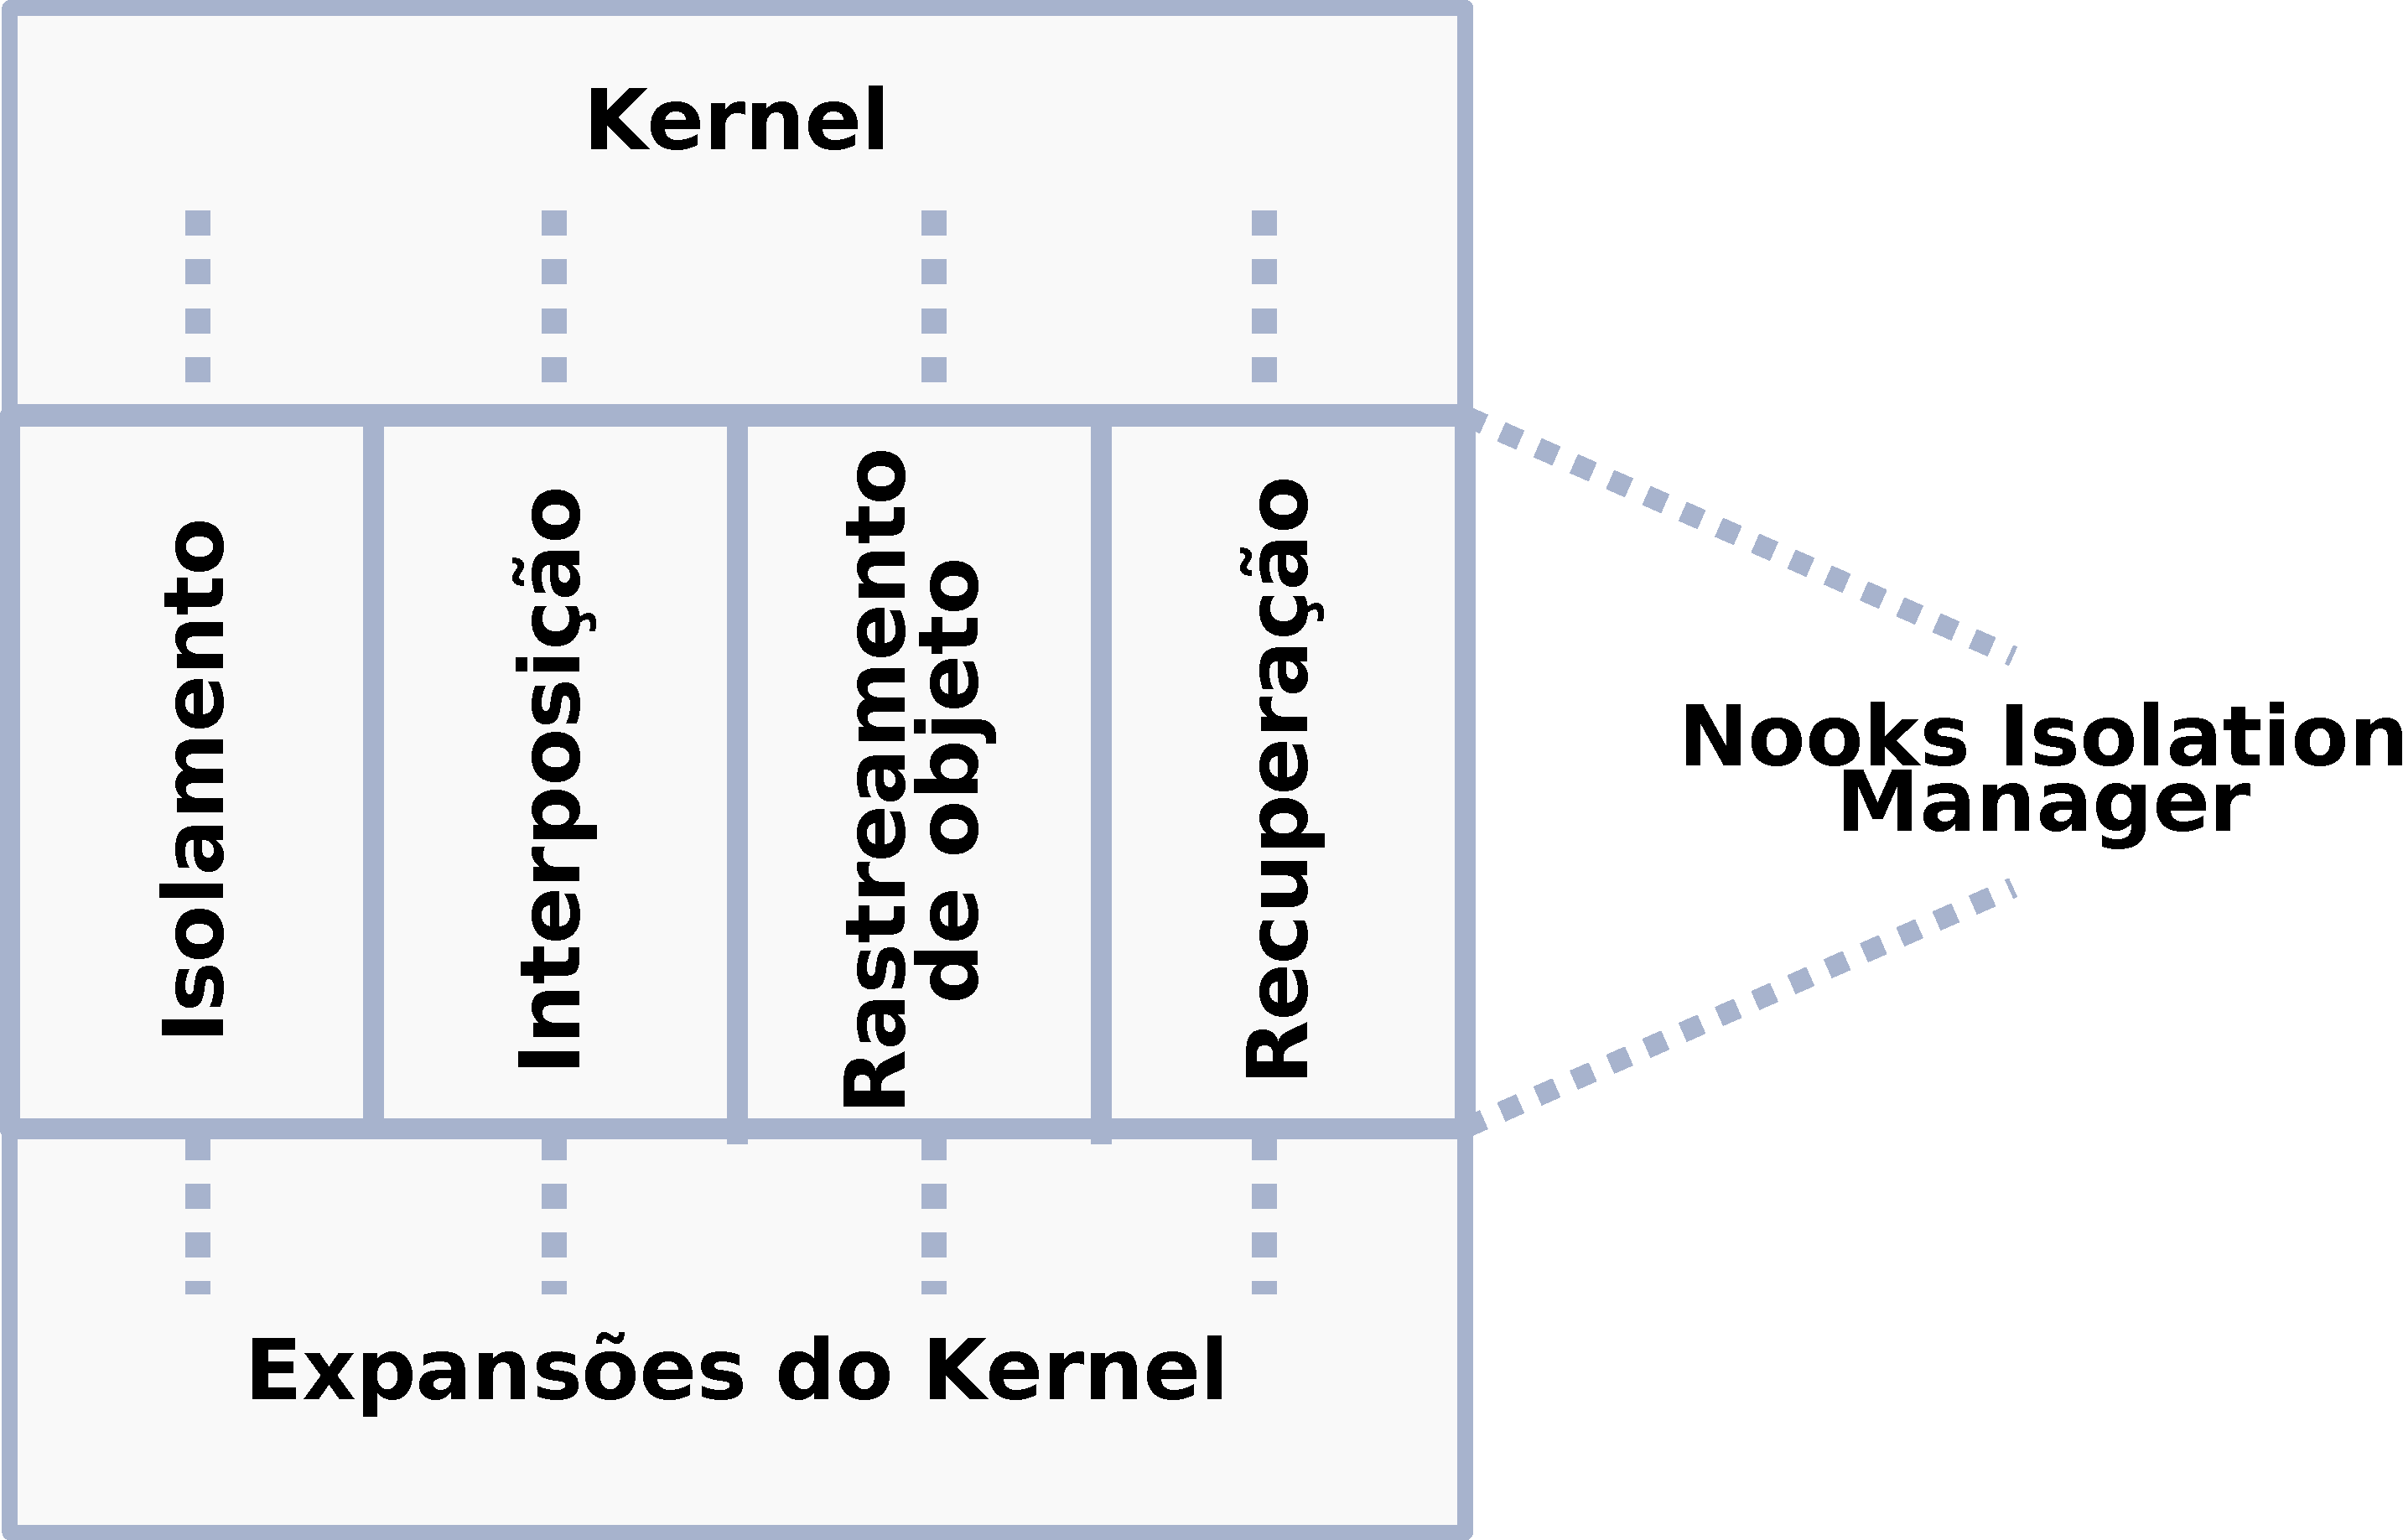
\includegraphics[width=0.8\textwidth]{nooks_nim}
	\caption[Visão geral da arquitetura do Nooks]{Visão geral da arquitetura do Nooks \citep{nooks}}
  \label{fig:nooks_nim}
\end{figure}

A Figura \ref{fig:nooks_nim} ilustra de forma geral a arquitetura de
\emph{Nooks}. Note que a comunicação entre o Kernel e as extensões (e vice-versa)
precisa passar pelo \emph{Nooks}. Esse intermédio é conduzido pelo \emph{Nooks
Isolation Manager (NIM)}, que é o responsável por implementar os objetivos do
projeto. \emph{Nooks} precisa estender-se em parte para o Kernel e em parte
para as extensões. No Kernel, é preciso alterar aquelas funções que são
disponibilizadas para as extensões ou que interagem com os módulos. Felizmente,
esse tipo de função pode ser detectado por algum padrão que, por sua vez, pode
ser abstraído para um \emph{script}. Além disso, esse tipo de modificação precisa ser
feito uma única vez. Do ponto de vista dos módulos, no geral, são poucos os
casos que precisam ser alterados diretamente, uma vez que eles fazem uso dos
recursos fornecidos pelo Kernel. Normalmente, módulos que exportam estruturas
de dados para o Kernel e o espaço de usuário também precisam ser alterados.

O \emph{Nooks} fornece isolamento por meio do LKPD: toda extensão
adicionada ao SO executa dentro do seu próprio LKPD que, por sua vez, é chamado
de \emph{contexto de execução}. Os domínios utilizam o mesmo nível de proteção
fornecido pelo processador para o Kernel, com a diferença de que o acesso de
escrita para certas porções é limitada e gerenciada pelo \emph{NIM}. Neste
sentido, podemos dividir o esquema de isolamento de \emph{Nooks} em duas partes:
o gerenciador de memória e o \emph{Extension Procedure Call} (XPC).

\begin{figure}[!h]
  \centering
  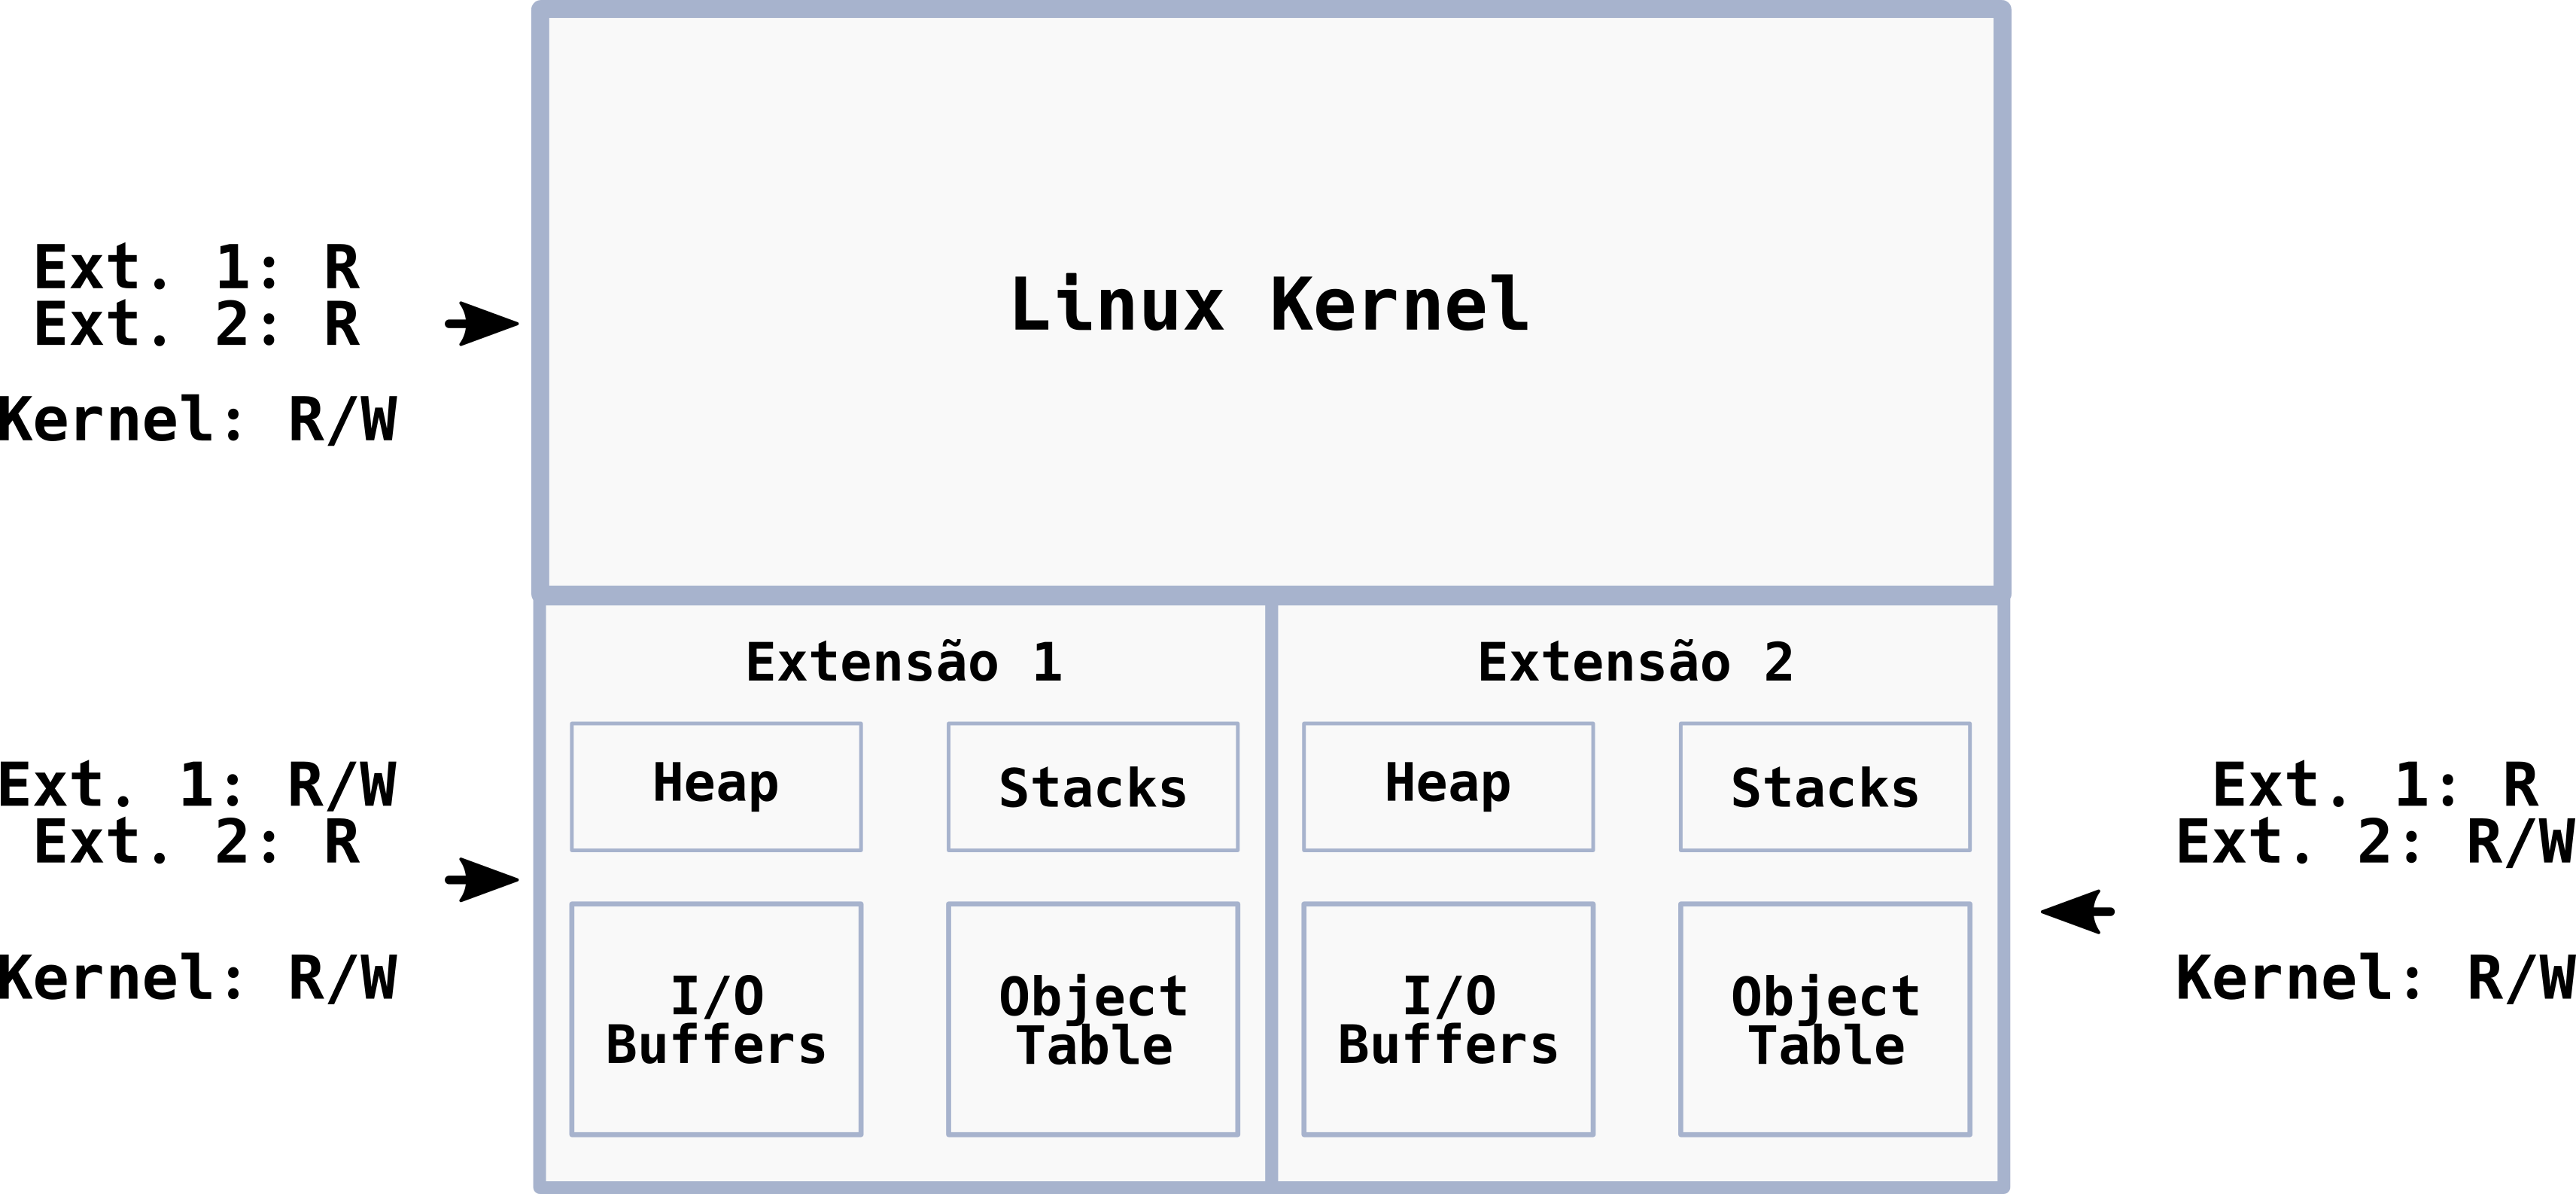
\includegraphics[width=0.8\textwidth]{nooks_mem}
  \caption[Acesso à memória do Nooks]{Acesso à memória do Nooks \citep{nooks}}
  \label{fig:nooks_mem}
\end{figure}

O gerenciador de memória de \emph{Nooks} é responsável por alocar, desalocar e
manipular os LKPDs. A Figura \ref{fig:nooks_mem} ilustra o \textit{kernel
address space}: note que o Kernel tem permissão de escrita e leitura sobre toda
a memória, mas os LKPDs mostrados só têm acesso de leitura e escrita a si mesmos.
A leitura de outras regiões de memória de dentro de um LKPD depende do controle
de acesso feito pelo NIM mas, no geral, só é permitida a leitura de outras
regiões da memória.

O outro mecanismo de isolamento fornecido pelo \emph{Nooks} é o XPC, que atua
como um serviço de transferência de controle criado para isolar as operações
feitas dentro do Kernel. A transferência de controle pode acontecer em duas
vias: do Kernel para a extensão (\texttt{nooks\_driver\_call}) e da extensão
para o Kernel (\texttt{nooks\_kernel\_call}). Essas funções esperam
três argumentos: um ponteiro para a função que será executada, uma lista de
argumentos e o domínio em que será executada. Toda vez que a rotina de
transferência é chamada, o contexto da stack que realizou a chamada é salvo e o
\emph{Page Table} para o novo domínio alvo carregado.

Um dos objetivos do \emph{Nooks} é o de ser usado em SOs de produção. Para isso,
ele tem de se integrar com o SO de forma a causar o menor impacto possível
nas extensões. Por isso, \emph{Nooks} isola as extensões com XPC e também
implementa um mecanismo de rastreamento de estruturas de dados chamado
\emph{object-tracking} (parte do \emph{NIM}). O \emph{object-tracking} tem três
recursos básicos: (1) manter uma lista de estruturas de dados do Kernel que são
manipuladas por uma extensão, (2) controlar todas as modificações para essas
extensões e (3) fornecer informações de objetos para limpeza de dados quando a
extensão falhar. O rastreamento dos objetos começa com o armazenamento de todos
os objetos em uso por uma extensão e em seguida é feita uma associação entre o
Kernel e as versões das extensões.

Por fim, \emph{Nooks} possui um mecanismo de recuperação que busca detectar
falhas de software quando uma extensão é chamada de forma inapropriada ou se
uma extensão está consumindo muitos recursos. A estratégia de recuperação é
subdividida em duas partes: \emph{recovery management} e \emph{user-mode
agent}. O primeiro é responsável por desalocar recursos e, se necessário,
realocá-los. O segundo é quem coordena a ação de recuperação e
é definido no espaço de usuário. Note que a flexibilidade do \emph{agent-mode}
permite várias possíveis formas de recuperação, sendo a mais direta forçar a
remoção da extensão, seguida da reinserção e em seguida prosseguindo com a
execução da aplicação.

\emph{Nooks} utilizou uma base de dados de inserção de falhas em módulos para
validar a sua eficácia, conseguindo tratar 99\% dos casos. Além disso, os
autores também validaram o trabalho da perspectiva do desempenho e notaram que,
na maioria dos casos, os gastos com a estrutura são compensados pelas vantagens.

\section{Mondrian Memory Protection e Mondrix}

\citet{mmp} buscaram explorar técnicas para realizar controle fino sobre da
memória, com o objetivo de adicionar mais confiabilidade e segurança para os
SOs. Os autores discutem os problemas associados com a decisão usual de se promover
isolamento por meio da separação do espaço de endereçamento dos processos, que
por sua vez faz com que todas as \emph{threads} de um processo compartilhem um
mesmo domínio de proteção. Além disso, o modelo de paginação comumente adotado impõe um
tamanho fixo de página. Logo, o menor compartilhamento possível é o de uma página, que
tem o mesmo nível de permissão para todos os elementos contidos nela. Os autores
argumentam que, apesar das vantagem oferecidas pelo modelo atual, muitos
aspectos de segurança e estabilidade do sistema são comprometidos. Dois
exemplos são apontados pelos autores; o primeiro ilustra o caso do servidor
Apache, que pode carregar vários \textit{plugins} externos, contudo, se algum
código malicioso ou defeituoso for carregado ele comprometerá toda a
estabilidade do servidor (em alguns casos quebrando a aplicação). Outro exemplo
refere-se ao acesso de ponteiros em outros domínios da memória (por exemplo,
acesso do espaço de usuário para o do Kernel), que atualmente não são permitidos,
sendo necessário realizar operações de cópias.

\begin{figure}[!h]
  \centering
  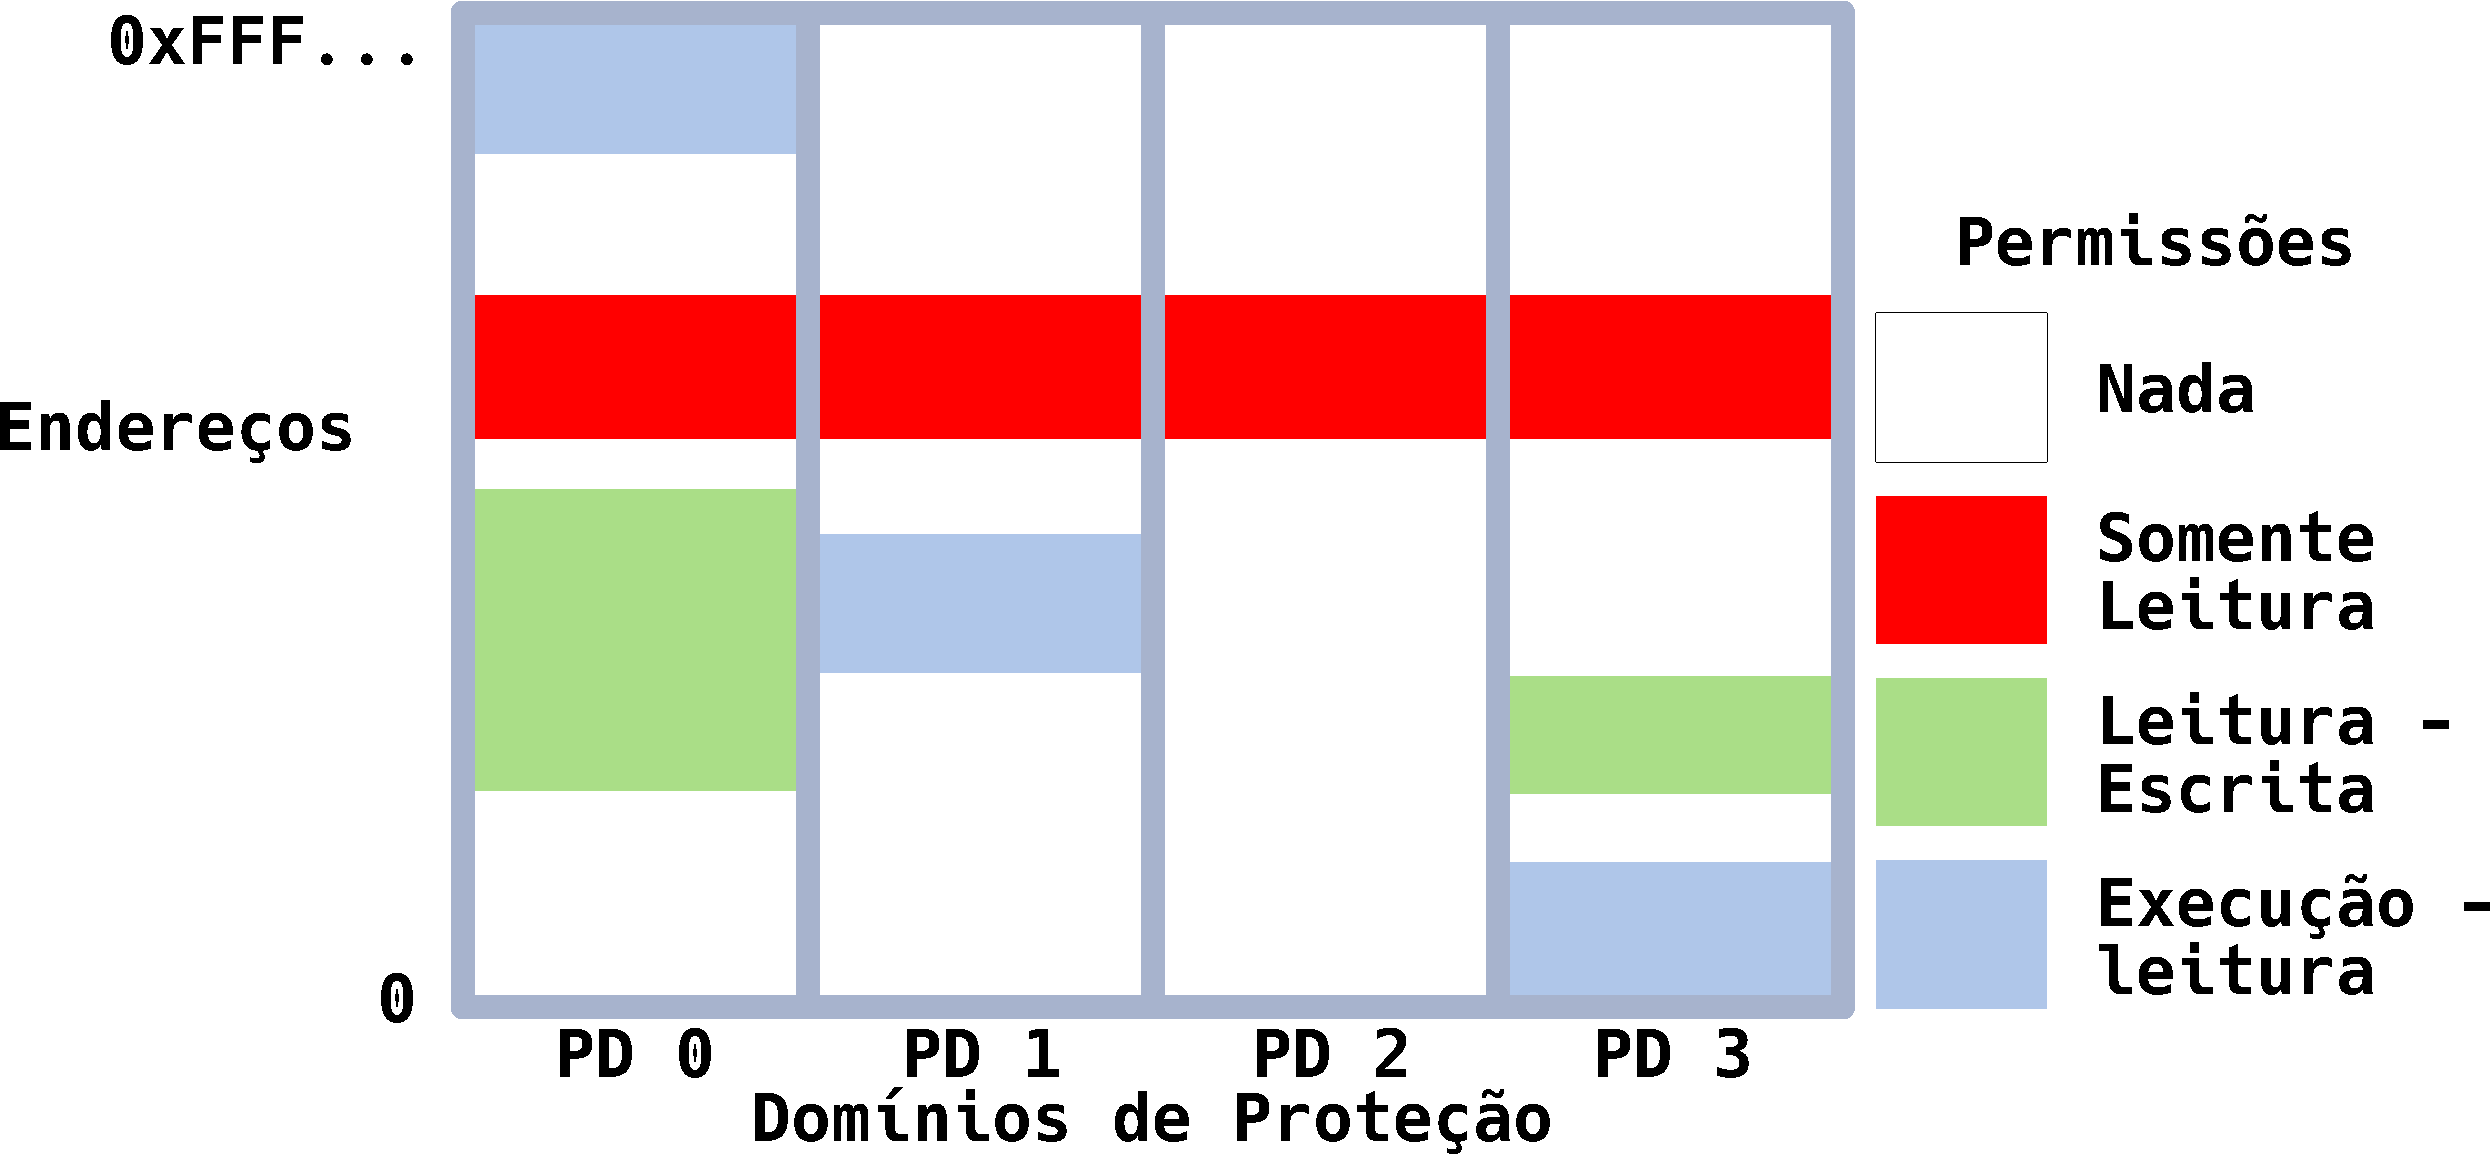
\includegraphics[width=0.7\textwidth]{mondrix_pd}
	\caption[Representação dos domínios de proteção do Mondrix]{Representação dos domínios de proteção do Mondrix (\cite{mondrix})}
  \label{fig:mondrixPD} 
\end{figure}

Os autores defendem que mecanismos de controle fino do acesso à memória podem
trazer grandes benefícios em termos de segurança, confiabilidade e, em certos
casos, desempenho. Nesse sentido, \citet{mmp} propuseram uma abordagem
que permite o controle de acesso à memória no nível do tamanho das palavras de
dado. Para isso é apresentado um novo tipo de abordagem baseada em hardware e
software chamado \emph{Mondrian Memory Protection (MMP)}~\citep{mmp}. Além
disso, uma implementação prática chamada \emph{Mondrix}~\cite{mondrix} foi
feita no GNU/Linux. A Figura~\ref{fig:mondrixPD} resume a representação de
memória que o MMP busca atingir. Repare que não existem porções de memória
específica; a memória é dividida em diversos compartimentos chamados
\emph{Protection Domains (PD)}. Um PD é definido como um contexto que determina
a permissão para executar um código. Cada PD é independente do espaço de
endereçamento e pode conter múltiplas \emph{threads}, mas cada \emph{thread} só
pode pertencer a um único PD.  O projeto do MMP é guiado por três requisitos:

\begin{enumerate}
	\item \textbf{Diferente}: Cada PD diferente pode ter um domínio distinto
				para a mesma região de memória;
	\item \textbf{Pequeno}: A granularidade de compartilhamento deve ser menor
				do que uma página;
	\item \textbf{Revogável}: Um PD é dono da sua própria região de memória e
				pode mudar a forma como outros domínios veem a sua memória.
\end{enumerate}

% TODO: FIGURA K
Os autores afirmam que MMP tem a semântica da segmentação (Seção ~\ref{sec:segmentacao}) sem os problemas
associados a ela. MMP fornece controle fino sobre a proteção dos dados
compartilhados, utiliza endereçamento linear, é compatível com o conjunto de instruções
existentes, não necessita de registradores de segmentos, possui um mecanismo
simples de revogação de permissões e não tem ponteiros marcados. Para que
MMP possa garantir o controle de acesso à memória, ele precisa verificar as
permissões de acesso feitas por cada operação de \emph{load/store}; isto
claramente consome mais recursos computacionais. Por isso, MMP é uma solução
que também depende da utilização de um hardware personalizado.

% TODO: FIGURA G -> A princípio não me parece que falar do hardware é útil...
%\hltodo[A Figura G]{Segmentation Fault} ilustra a arquitetura de hardware proposta para a implementação do
%MMP; note que ela introduz muitos elementos novos. %TODO: Descrever o hardware

Da perspectiva do software, Mondrix \citep{mondrix} sugere a utilização de um
novo elemento chamado de Supervisor de Memória, dividido em duas partes:
uma parte superior, responsável pelo controle do acesso; e parte inferior, responsável
por escrever nas tabelas de permissão. A parte superior é a mais importante,
sendo responsável por manter e controlar as políticas, pela interface com o Kernel,
por rastrear objetos compartilhados e por implementar grupos de permissão. As
definições de permissão da memória são descritas por três elementos:

\begin{enumerate}
	\item \emph{Permissão de Acesso}: As permissões de acesso são definidas pelo
				seguinte conjunto de elementos: permissão do domínio, \emph{gates},
        tabela de \emph{stack};
	\item \emph{Dono da Memória}: Define quem tem autoridade sobre a região de
				memória (domínio). Note que o espaço de endereçamento é contínuo e sem
				sobreposição, logo, cada região tem apenas um dono;
	\item \emph{Permissões Exportadas}: É possível exportar as permissões de
				acesso, permitindo que outras regiões chamem códigos
				fora do seu domínio. Contudo, a exportação pode ser controlada, de forma
				que outros trechos que acessem o código tenham uma visão limitada da
				região.
\end{enumerate}

Dados esses elementos, o Supervisor de Memória atua tomando as decisões
referentes ao acesso a uma dada região da memória.

Um aspecto interessante de se notar do Supervisor de Memória é a sua separação
lógica do alocador de memória. Mondrix permite que o Kernel escolha qual
alocador de memória deseja utilizar; isso é possível porque um domínio solicita
memória para o alocador e o Supervisor só estabelece as permissões para a
memória solicitada.
% Gosto muito dessa ideia de separar o alocador do controlador de acesso à
% memória, na minha opinião em termos práticas essa é uma das ideias mais
% valiosas desse trabalho.

O Supervisor também é responsável por revogar permissões quando uma região de
memória é liberada, além de manter o rastreamento de qual domínio tem acesso a
qual região de memória. O Supervisor ainda gerencia o acesso à \emph{stack}
das \emph{threads} (uma \emph{thread} só pode controlar \emph{stacks} que estão
no seu domínio), cria e destrói proteções de domínio e também valida as
políticas de acesso.

\section{SpaceJMP}
\label{sec:mvas}

Toda vez que um processo é criado, ele inicializa diferentes estruturas de
dados relacionadas à sua execução. Um dos elementos fundamentais dos processos
é o espaço de endereçamento virtual (\emph{Virtual Address Space -- VAS}), que é
completamente acoplado aos processos. Normalmente, os VAS são maiores que a
memória física e são totalmente isolados de outros processos. Se um processo
precisar compartilhar dados com outros processos, será necessário criar e
gerenciar uma região de memória compatilhada que permita a escrita e/ou leitura
por outros processos. O atual modelo de VAS não dá suporte para
o compartilhamento de estruturas de dados entre processos com base em ponteiros;
normalmente, é necessário serializar os dados, o que tem se tornado um incômodo.

\begin{figure}[!h]
  \centering
  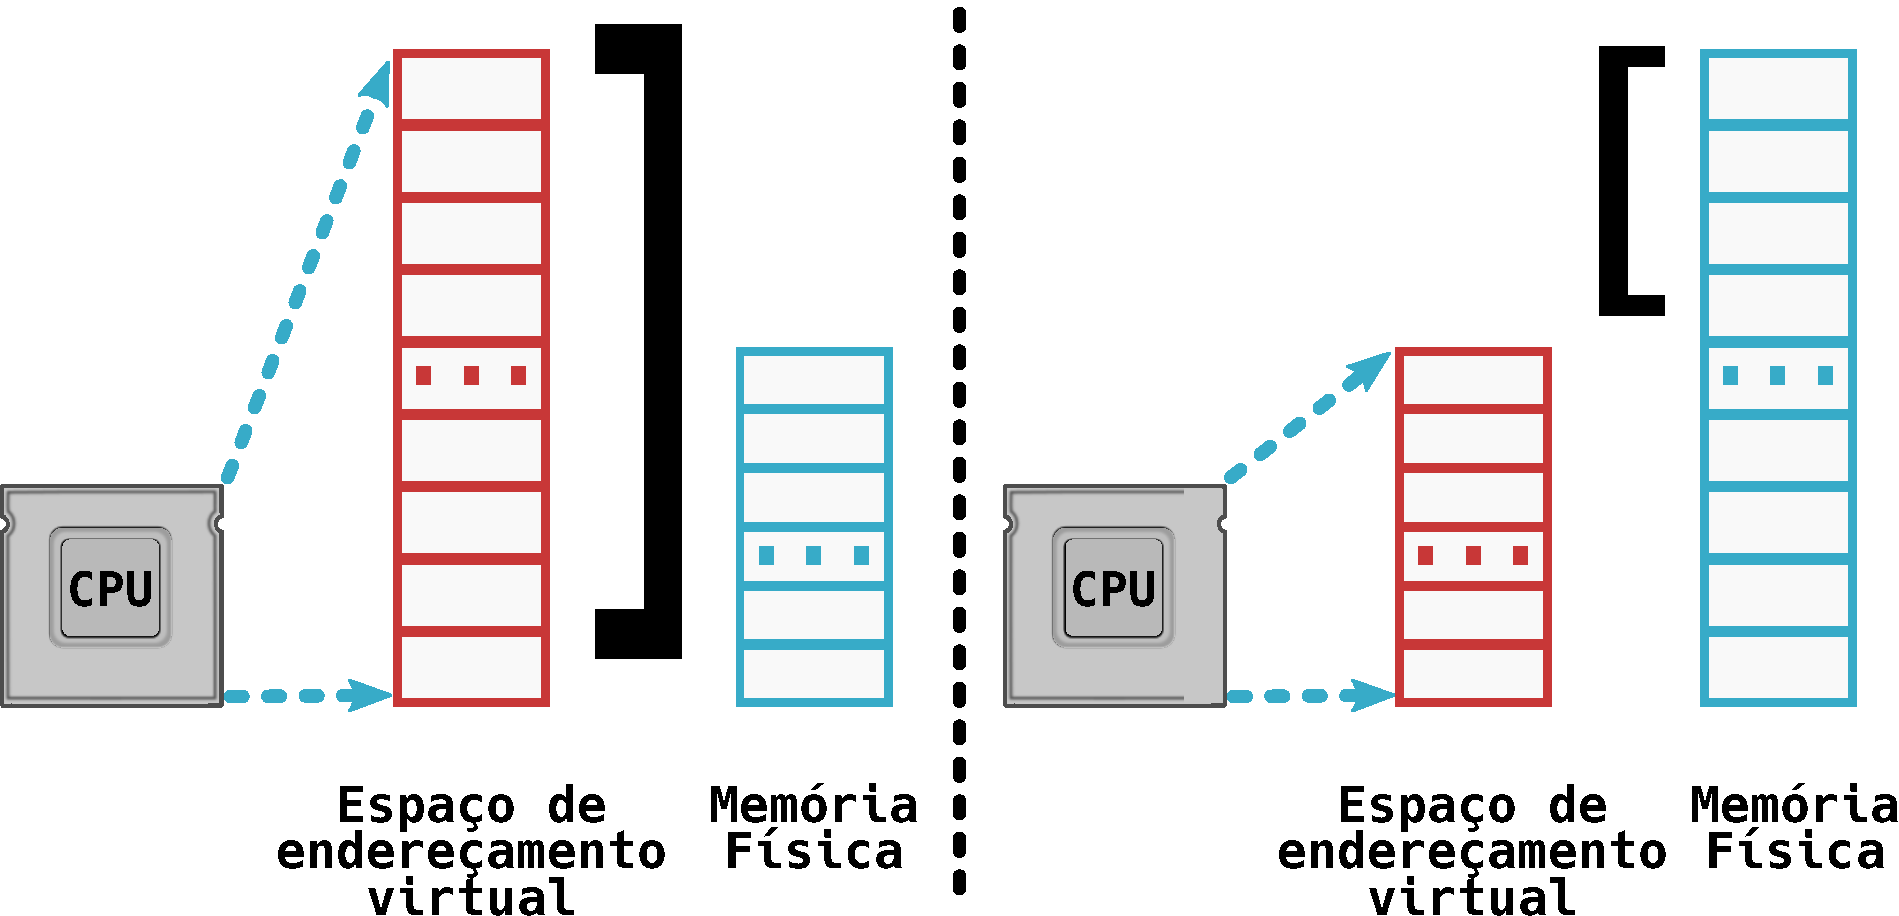
\includegraphics[width=.7\textwidth]{vas_vs_physical_address} 
  \caption{VAS e Memóra Física}
  \label{fig:vas_vs_physical} 
\end{figure}

No início dos anos 1990s, os processadores tinham poucos bits para o VAS, mas que eram suficientes
para endereçar toda a memória física disponível na época. Apesar disso, durante
esse período, o tamanho da memória cresceu consideravelmente e os processadores
não foram mais capazes de endereçar diretamente todo o endereço de memória disponível
\cite{crowley}. A Figura \ref{fig:vas_vs_physical} exemplifica o problema
mencionados acima: a parte da esquerda ilustra uma CPU com bits suficientes
para o VAS, que consegue endereçar todo o espaço de endereçamento
físico da memória. O lado direito da figura representa uma situação na qual o
VAS é menor do que a memória física. Assim, um um único processo não é capaz de
acessar toda a memória física disponível, impondo um limite ao processo
quanto ao tamanho que ele pode ter. Essa situação
não é uma novidade: enquanto a indústria não produzia
novos processadores com bits extras para elevar o tamanho da VAS, os
desenvolvedores tiveram que utilizar vários artifícios para superar o
problema de bits insuficientes. Hoje em dia, esse problema está sob controle,
uma vez que os processadores atuais possuem um grande espaço de endereçamento.
Contudo, estamos no início de uma geração da computação conhecida por
\emph{data-centric}, que será dominada por grandes memórias não-voláteis
\citep{outlook}. Assim, simplesmente incrementar o total de bits para o VAS nas
CPUs não sanará tão facilmente esse problema, pois elevar o número de bits na
VAS tem impactos na produção, desempenho e consumo de energia \citep{spacejmp}.

Um dos problemas do modelo de processos atual é a representação
das estruturas de dados baseadas em ponteiros fora dos
limites dos processos. A serialização de dados ou ponteiros especiais podem ser
empregados para resolver este problema, contudo, ambos os métodos são
incômodos, ineficientes e, em muitos casos, confusos \citep{spacejmp}. O segundo
problema está associado com a tarefa de coordenar o compartilhamento de memória
entre vários processos, uma vez que esta é uma tarefa complicada e tediosa.

Para tentar resolver os problemas citados, \citet{spacejmp} propuseram uma
técnica chamada \emph{SpaceJMP}. Os autores propõem desacoplar o VAS dos
processos e permitir que um único processo tenha Múltiplos VAS (MVAS)
associados a si. Nesse contexto, o VAS é promovido para um objeto de
primeira-classe no SO e dá ao processo a habilidade de gerir os muitos
VAS.

\begin{figure}[!h]
  \centering
  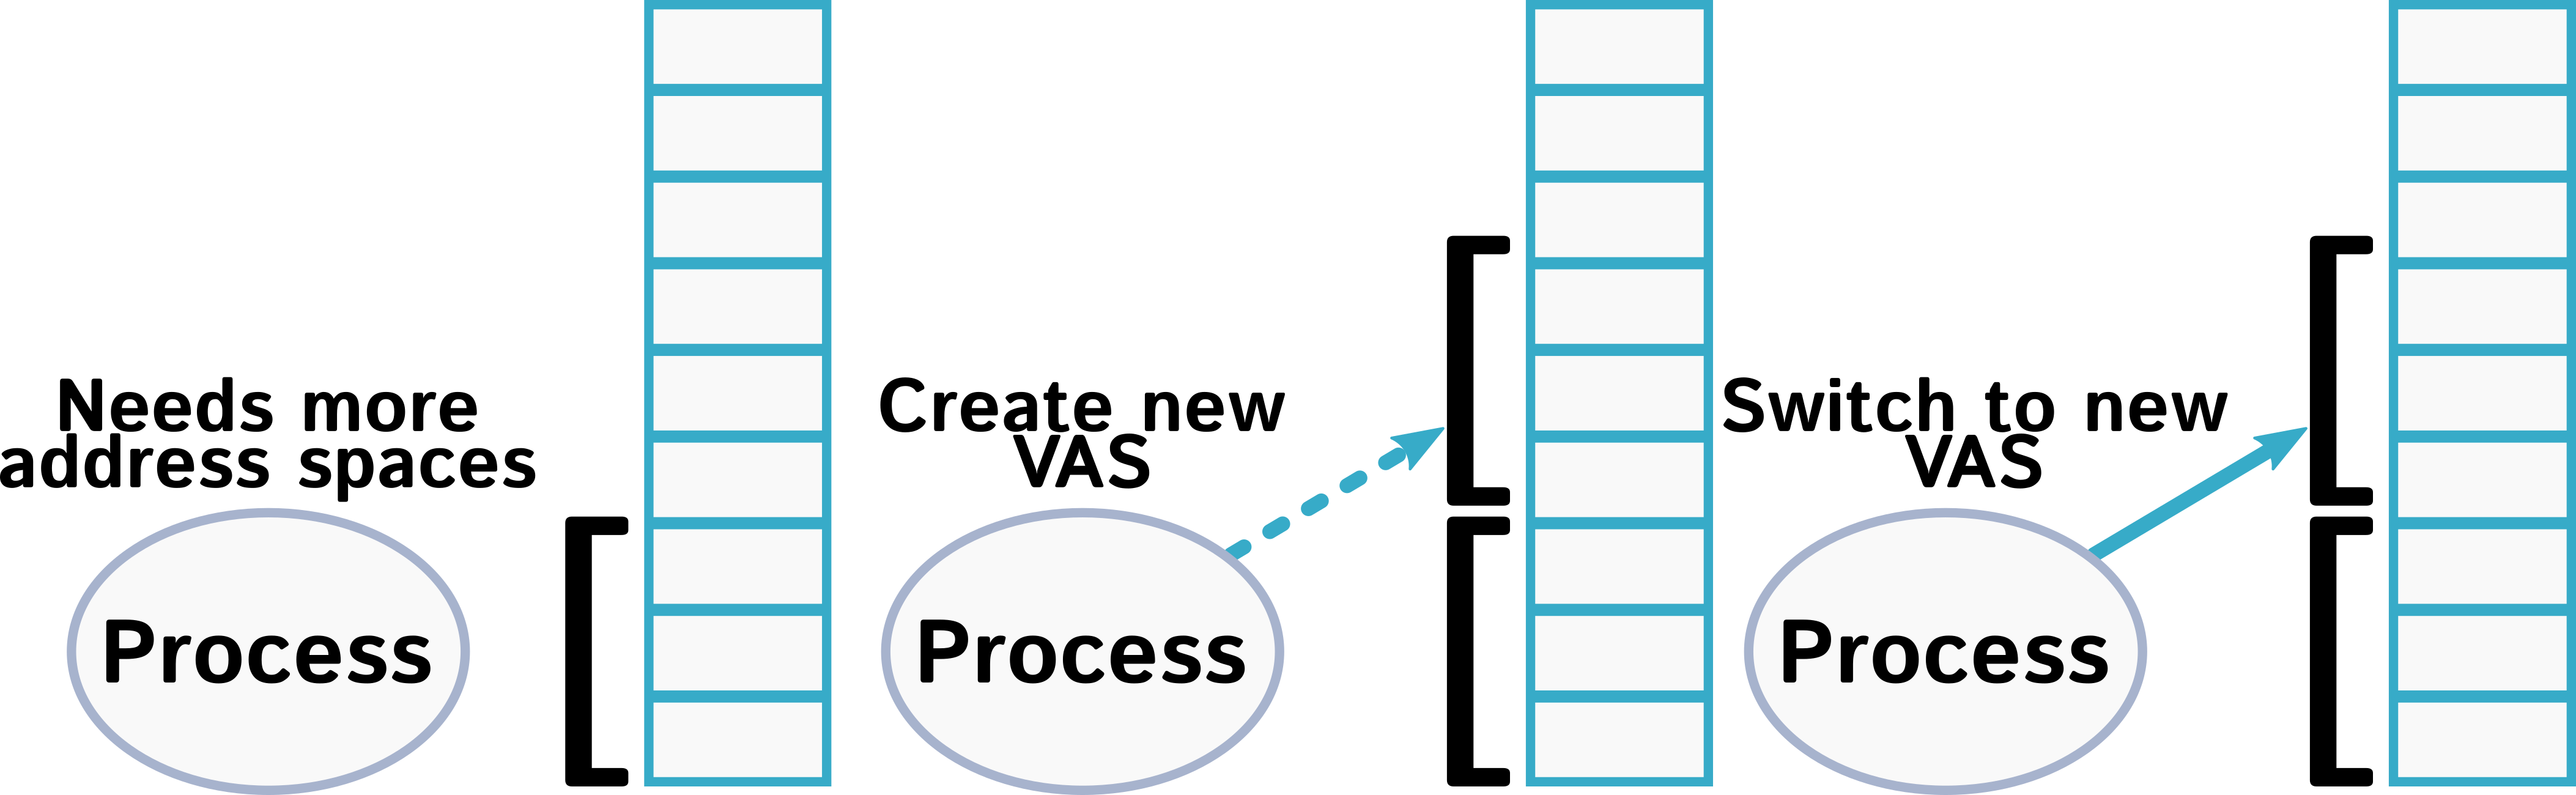
\includegraphics[width=.7\textwidth]{solve_huge_address_memory}
  \caption{Resolvendo o problema de endereçar memórias físicas grandes}
  \label{fig:large_memory}
\end{figure}

A Figura \ref{fig:large_memory} ilustra como MVAS resolve o problema de
endereçar memórias físicas maiores do que o VAS. Basicamente, todo processo
pode criar múltiplas VAS e alternar entre eles. Se os processos precisarem de
mais memória do que o disponível, basta criar um novo espaço de endereçamento
com o começo apontando para uma região de memória não utilizada e, em seguida,
anexar o novo VAS ao processo. O problema da serialização e compartilhamento de
dados também pode ser simplificado pelo MVAS: basta criar um VAS e permitir que
múltiplos processos se anexem a ele.

\begin{figure}[!h]
  \centering
  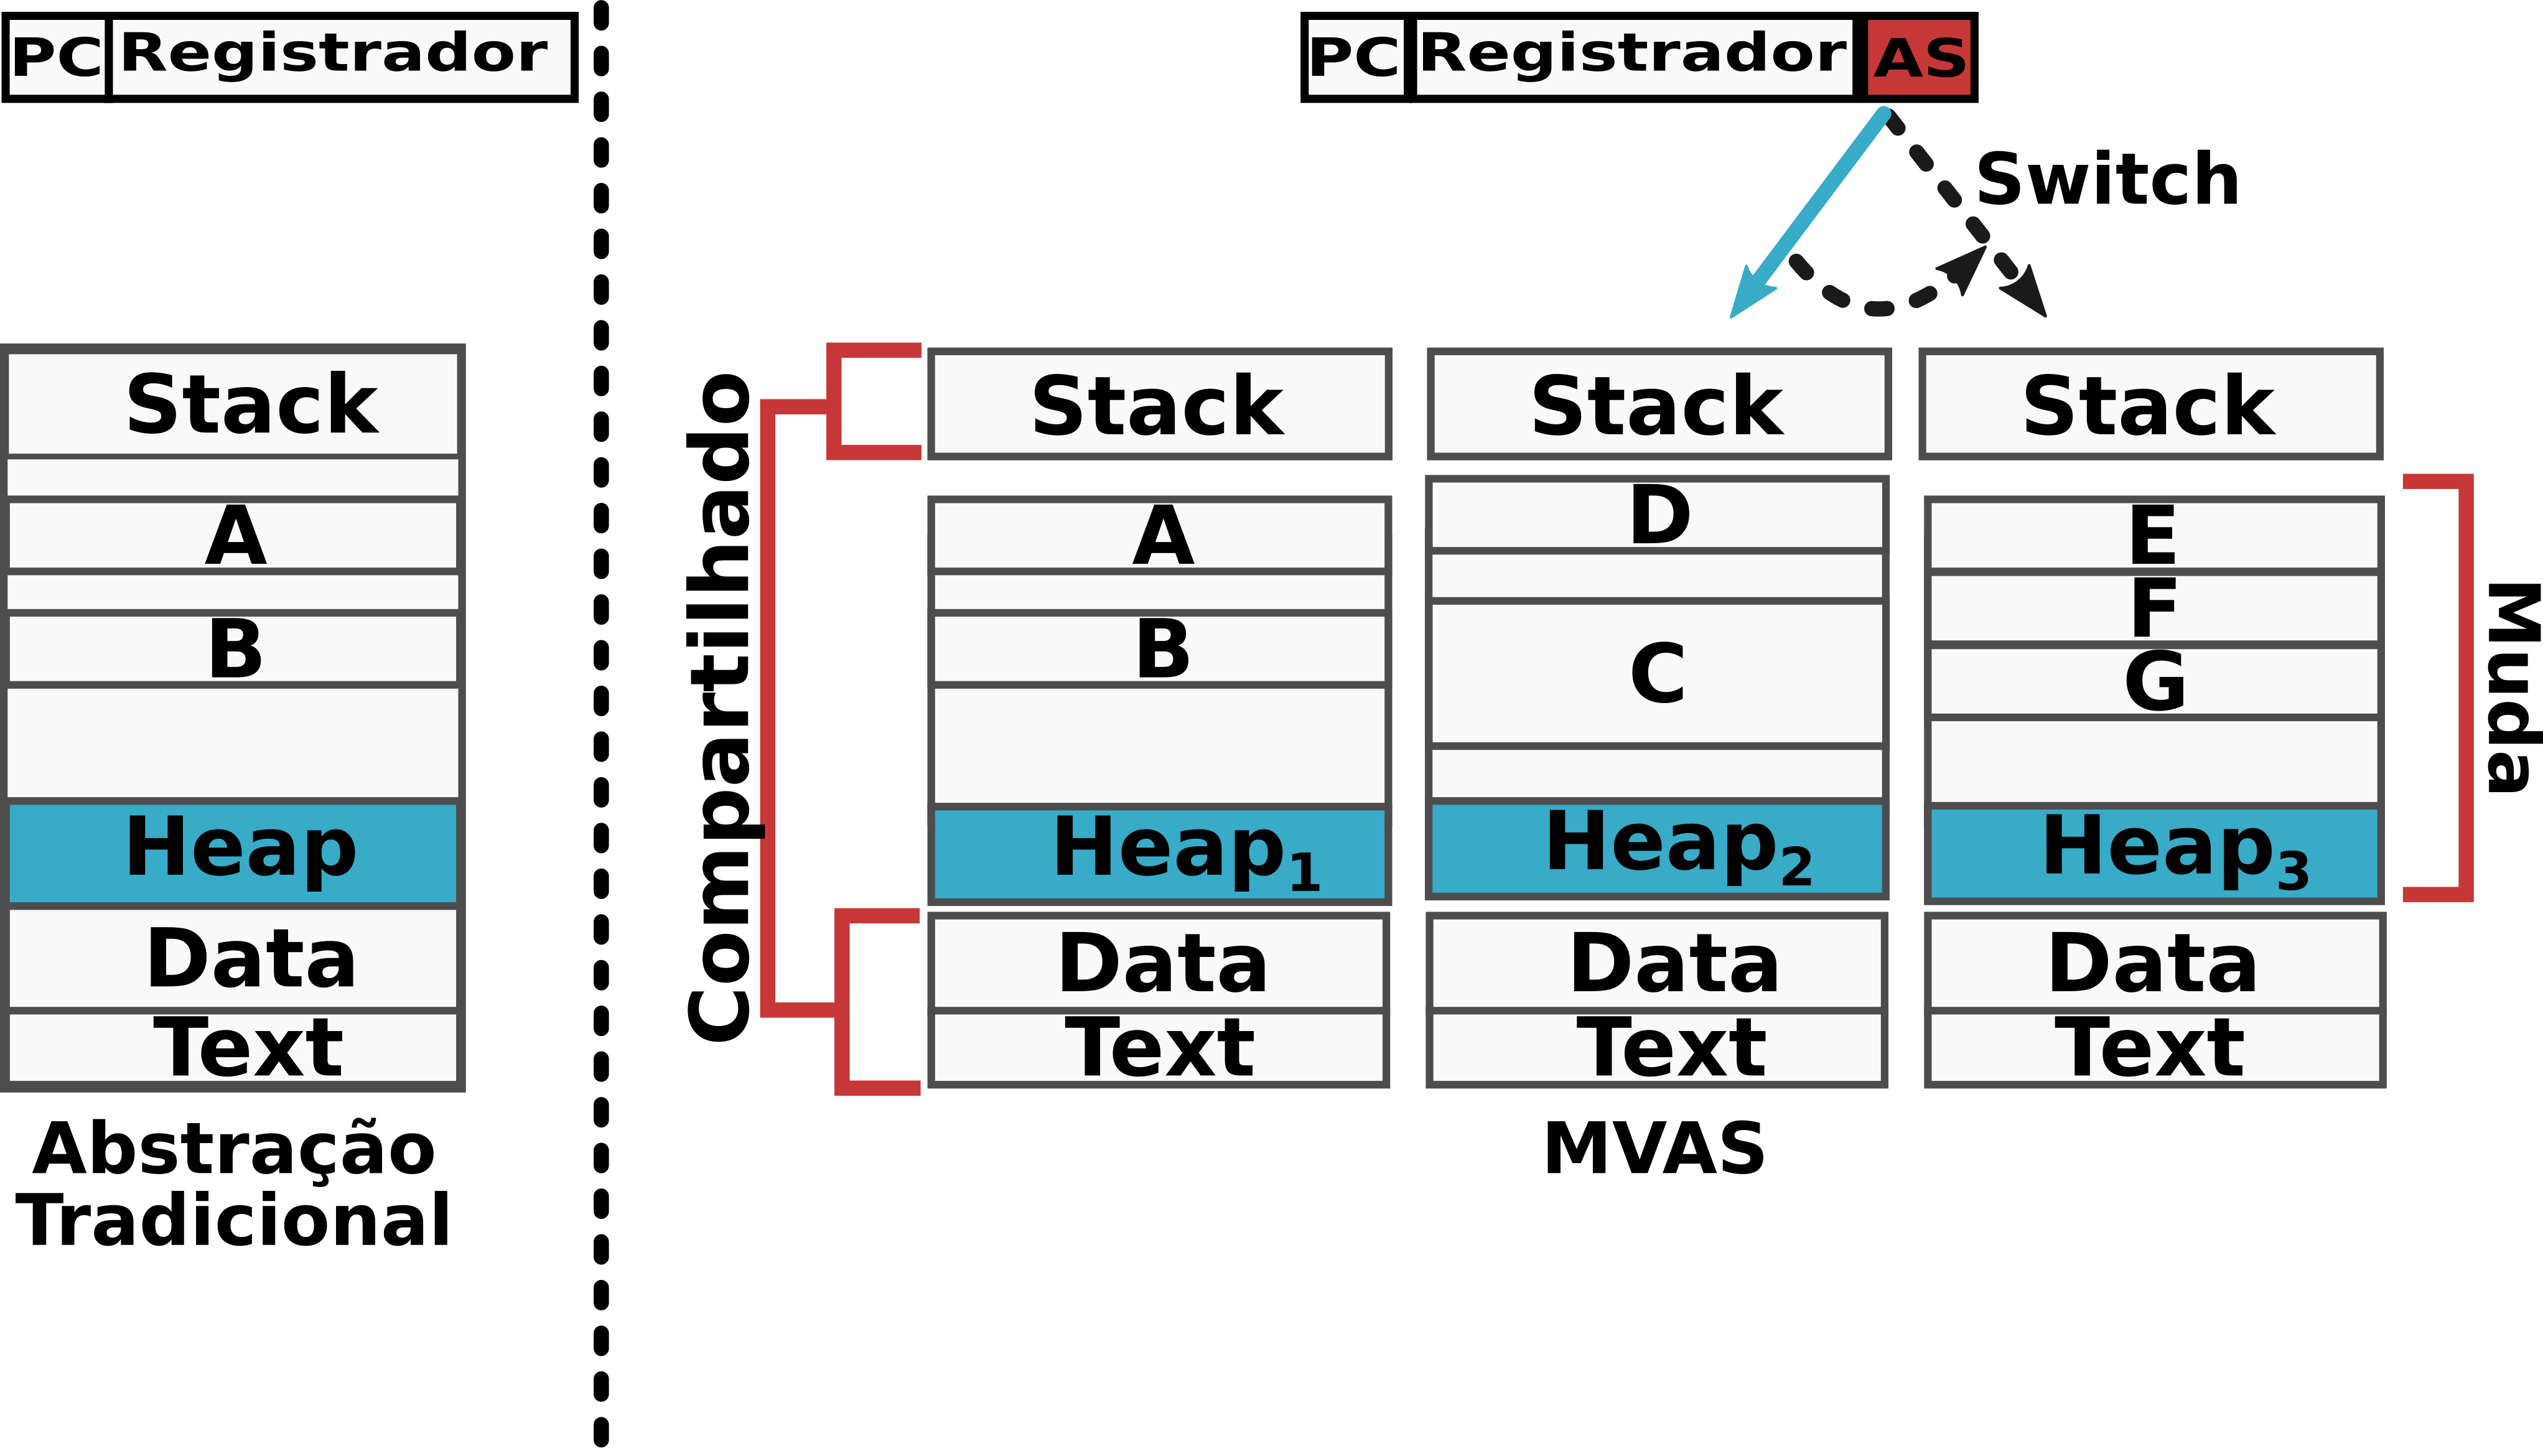
\includegraphics[width=.7\textwidth]{traditional_vs_mvas} 
	\caption[VAS e MVAS]{VAS e MVAS \citep{spacejmp}}
  \label{fig:traditional_vs_mvas} 
\end{figure}

A Figura \ref{fig:traditional_vs_mvas} ilustra a principal diferença entre um
processo com um VAS acoplado para um modelo no qual o VAS é desacoplado
(MVAS). O lado esquerdo da Figura mostra um processo tradicional, como explicado
na Seção \ref{sec:processos-e-threads}. O lado direito da figura representa um
processo com múltiplos VAS e diferentes informações dentro de cada \emph{Heap}
e segmentos de memória. Nesse novo cenário, a pilha, os dados e os segmentos
de texto são compartilhados entre os vários MVAS. Por fim, é importante
notar que os processos precisam manter a informação sobre o VAS atualmente em
execução.
 
Os autores da técnica fizeram uma implementação para GNU/Linux. A principal
funcionalidade do MVAS foi exposta para o usuário via \emph{system calls}. A
lista a seguir mostra o conjunto de funções expostas para o usuário:

\begin{itemize}
  \item \texttt{vas\_create()}: Cria um novo VAS com o nome indicado;
  \item \texttt{vas\_delete()}: Remove um VAS criado previamente;
  \item \texttt{vas\_find()}: Encontra um VAS de acordo com o nome;
  \item \texttt{vas\_attach()}: Anexa um VAS ao processo;
  \item \texttt{vas\_detach()}: Desanexa um VAS do processo;
  \item \texttt{vas\_switch()}: Muda o VAS atualmente instalado no processo para outro.
\end{itemize}

\begin{figure}[!h]
  \centering
  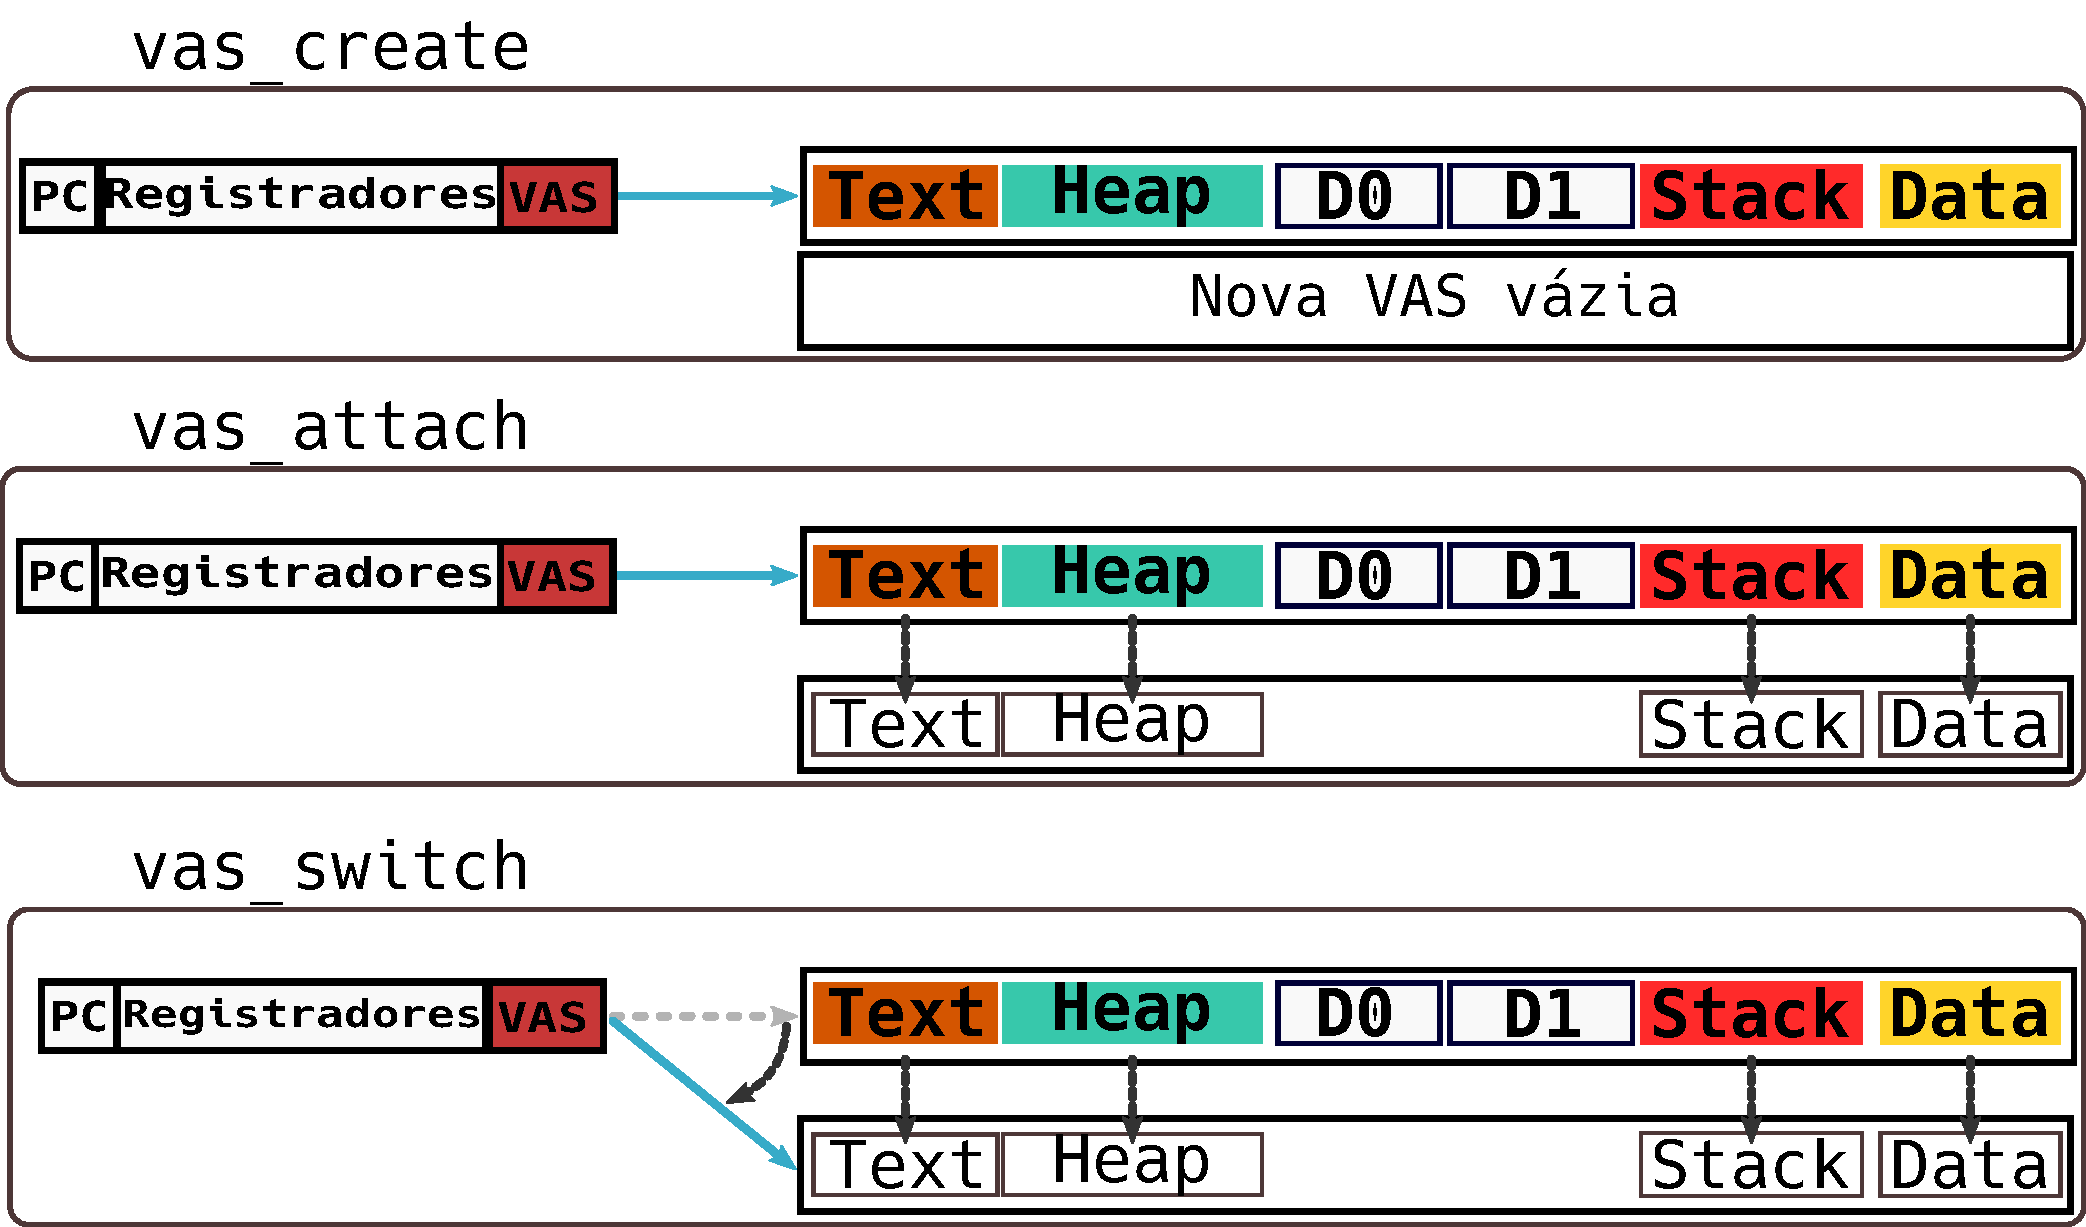
\includegraphics[width=.7\textwidth]{mvas_example} 
	\caption[System Call disponibilizada pelo SpaceJMP]{System Call disponibilizada pelo SpaceJMP \cite{ellarge}}
  \label{fig:mvas_example}
\end{figure}

A Figura \ref{fig:mvas_example} ilustra o comportamento das chamadas de sistema
implementadas. O topo da figura mostra um processo normal com um VAS padrão
associado a si; em seguida, a chamada para a função \texttt{vas\_create()} é
feita de forma a criar um novo VAS. Após a criação, é preciso anexar o VAS ao
processo por meio da chamada de sistema \texttt{vas\_attach()}. Por fim, o
processo pode mudar entre os VAS por meio da chamada para
\texttt{vas\_switch()}.

\section{Light-weight Contexts}
\label{sec:lwc}

O fluxo de execução do processo é controlado pelo \textit{Program Counter (PC)}
juntamente com os dados da memória. Por sua vez, o escalonador é a entidade que
orquestra quando retirar e inserir um novo processo para execução na CPU. Consequentemente,
tanto o PC quando os demais dados do processo são mantidos juntos no nível do
kernel.

\citet{litton} afirmam que o desacoplamento do isolamento da memória, estado de
execução e separação dos privilégios dos processos trazem benefícios. Com tal
ideia em mente, os atores sugerem uma nova abstração de processos chamada de
\textit{lightweight-context (lwC)}. Basicamente, cada processo pode ter um
(lwC root) ou mais lwCs, cada um com o seu próprio mapeamento
virtual da memória, descritor de arquivos e credenciais. Opcionalmente, a API
do lwC permite controlar quais elementos podem ser compartilháveis ou não entre
os lwCs.

Um lwC compreende um mapeamento de memória virtual, uma coleção de mapeamento
de páginas, \emph{bindings} de descritores de arquivos e conjuntos de
credenciais; sempre que um novo processo é criado, o sistema cria um novo lwC
para ele. A aplicação pode acessar todas as funcionalidades do lwC via espaço
do usuário através de chamadas de sistemas que fazem o controle fino dos
comportamentos fornecidos.

As chamadas mais interessantes são \texttt{lwCreate()} e \texttt{lwSwitch()}.
O \texttt{lwCreate()} tem uma semântica similar ao da chamada de sistema
\texttt{fork()}; assim que a chamada é feita, o processo pai tem os seus dados
duplicados no processo filho. Contudo, ao contrário do \texttt{fork()}, o
\texttt{lwCreate()} não cria uma nova \emph{thread} e nem um novo \emph{PID}.
Ao final da execução da chamada de sistema, o \texttt{lwCreate()} retorna um
identificador do novo contexto para o processo pai e se estiver no processo
filho ele retorna -1. A cópia do estado do processo pai na forma do contexto,
recebe o nome de \emph{snapshot}. Depois da criação do processo filho, a
aplicação é livre para fazer a troca (com o \texttt{lwSwitch()}) para algum de
seus \emph{snapshots} a qualquer momento.

A Figura \ref{fig:lwc} ilustra a operação de troca entre diferentes lwCs. Um
processo pode criar vários lwCs durante a sua execução e em
diferentes momentos e pode
seletivamente escolher transferir o seu fluxo de execução para outro lwC por
meio de uma chamada para \texttt{lwSwitch()}. A mudança da \emph{thread} é
feita pelo SO, que é responsável por mudar automaticamente o mapeamento da
memória virtual, as entradas das tabelas de arquivos, o PC e o \emph{stack
pointer}.

\begin{figure}[!h]
  \centering
  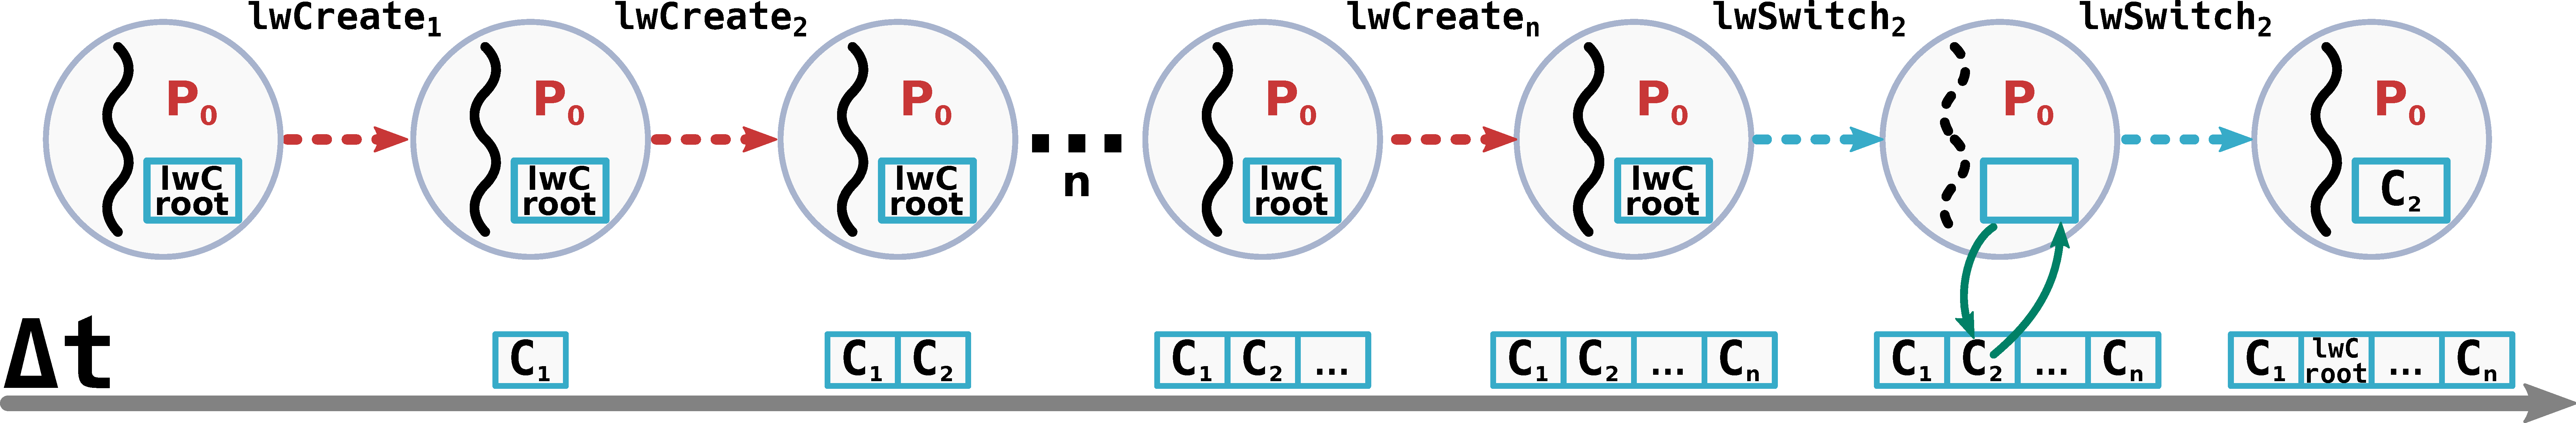
\includegraphics[width=\textwidth]{lwC} 
  \caption{Exemplo do comportamento do lwC}
  \label{fig:lwc} 
\end{figure}

A interface de lwC também permite que outras operações, como compartilhamento
dinâmico ou estático de recursos, controle sobre o acesso as
\emph{capabilities}, emulação de chamadas de sistema e novas camadas de
isolamento dentro do processo. Todo o conjunto de chamadas de sistema do lwC
fornece um sofisticado modelo de programação que permite novas capacidades
tais quais rápido \emph{roll-back}, isolamento de seções e compartimentos de
proteção. A API do lwC é composta das seguintes funções:

\begin{itemize}
  \item \texttt{lwCreate(resource-spec,options):} Cria um novo contexto de acordo com o estado atual do processo;
  \item \texttt{lwSwitch(target, args):} Alterna entre os diferentes contextos;
  \item \texttt{lwRestrict(l, resource-spec):} Permite restringir a forma de acesso ao contexto;
  \item \texttt{lwSyscall(target, mask, syscall, syscall-args):} Intercepta chamadas de sistema dentro de um contexto permitindo validar permissões de execução.
\end{itemize}

Os autores demonstram os conceitos do lwC em uma implementação no FreeBSD. As
modificações principais foram feitas no gerenciador de memória e estruturas de dados do
processo. Seu uso foi demonstrado em adaptações feitas no Apache, Nginx e
OpenSSH. Por fim, os autores propõem certos algoritmos que discutiremos no
Capítulo \ref{cap:analise-sobre-abstracoes-de-processos}.

\section{Exokernel}
\label{sec:exokernel}

\citet{exokernel} defendem que os projetos de SOs possuem uma série de
desvantagens por terem várias abstrações diretamente programadas no núcleo. Os
autores argumentam que as abstrações implementadas diretamente no SO possuem
sérios impactos no desempenho, reduz consideravelmente a flexibilidade das
aplicações e limita as possibilidades de ampliar as funcionalidade
disponibilizadas no espaço do usuário. A implementação dessas abstrações
diretamente no núcleo do SO são problemática uma vez que: impedem a aplicação
de tirar proveito das otimizações que são especificas do seu domínio, as
mudanças em tais abstrações são desencorajadas e reduzem as possibilidade do
que pode ser feito no espaço de usuário.

Segundo os autores, a fixação das abstrações de alto-nível apresentam as
seguintes limitações:

\begin{itemize}
  \item A degradação do desempenho ocorre uma vez que atender ao maior número
        de aplicações possível com a mesma abstração tem um custo
        computacional. Por exemplo, algumas aplicações podem sofrer com o
        \emph{overhead} gerado por outras camadas de abstrações na qual não
        precisa;
  \item As informações de utilização de recursos são escondidas das aplicações,
        isto dificulta a aplicação ter controle sobre os recursos utilizados;
  \item As aplicações ficam limitadas a utilizar apenas aquelas interfaces
        padrão fornecidas pelo SO.
\end{itemize}

Por fim, com esses problemas em mente e motivados pela antiga observação de que:
quanto mais baixo o nível das primitivas (simples), mais eficientemente ela
pode ser implementada e maior a amplitude de ação fornecida para abstrações de
alto-nível; os autores propuseram uma nova arquitetura de SO chamada
\emph{exokernel}.

\emph{Exokernel} busca ser um núcleo mínimo que permita multiplexar de forma
segura os recursos de hardware e ao mesmo tempo fornecer uma interface de
baixo-nível na qual as abstrações do SO podem ser construída sobre ela. Para
que seja possível implementar um SO usando este conceito é preciso implementar
a chamada \textit{biblioteca do SO} com acesso aos recursos de baixo nível e
com as abstrações construídas nela (e.g. processos, arquivos, escalonador,
etc). Para que a implementação de tal conceito seja possível, os autores os
seguintes princípios:

\begin{enumerate}
  \item \textbf{\emph{Expor o hardware de forma segura:}} O conceito
        fundamental do \emph{exokernel} consistem em exportar de forma segura
        e controlada o acesso de baixo nível ao hardware, por isto toda
        implementação do \emph{exokernel} deve concentrar-se em exportar os
        privilégios e recursos de máquina. Por isto ele não deve impor
        abstrações de alto-nível, i.e, o \emph{exokernel} deve evitar gerir
        recursos;
  \item \textbf{\emph{Expor alocações:}} Um \emph{exokernel} deve permitir que
        uma biblioteca de SO aloque recursos. Além disto, os recursos não devem
        ser implicitamente alocados uma vez que a biblioteca de SO tem a
        obrigação de participar de todas as decisões de alocação;
  \item \textbf{\emph{Expor nomes:}} Um \emph{exokernel} deve exportar nomes
        físicos. Isto é eficiente uma vez que reduz o nível de indireção, e por
        sua vez o número de traduções necessárias entre nomes virtuais e
        físicos. Por fim expor nomes físicos também encapsula atributos de
        recursos uteis, por exemplo, um sistema de caches fisicamente indexado
        e diretamente mapeado, tem o nome da página física (i.e. o número da
        página) determina qual página que conflita;
  \item \textbf{\emph{Expor revogações:}} Um \emph{exokernel} deve utilizar um
        protocolo de revogação de recursos explicitas para que a biblioteca do
        SO possa gerir os recursos de forma eficiente;
\end{enumerate}

Por fim, além desses princípios o \emph{exokernel} também deve especificar as
políticas para arbitrar a competição entre as bibliotecas do SO. Dado esses
princípios o \emph{exokernel} deve disponibilizar as seguinte tarefas: ligação
segura, visibilidade de recursos e protocolo de falha.

A ligação segura (\emph{Secure Bindings - SB}) é o mecanismo que desacopla a
autorização do uso dos recursos. Para implementar o SB é preciso um conjunto de
primitivas que a aplicação pode usar para expressar verificações de proteção.
Essas podem ser implementadas em hardware ou software, por exemplo, a entrada
da TLB é uma primitiva de hardware. Na prática o SB trabalha com o conceito de
"baixar o código para o kernel", esse código é chamado para cada acesso ou
evento do recurso para determinar o dono e a ação que o Kernel deve tomar.
Baixar o código dentro do kernel permite uma \emph{thread} da aplicação ter controle
sobre os eventos. Isto melhora o desempenho uma vez que elimina a camada
intermediaria do Kernel e também propícia limitar a aplicação aos seus
recursos.

A tarefa de \emph{revogação visível} é o mecanismo para recuperar os recursos
e romper com o SB estabelecidas. Vale observar que este mecanismo pode ser
visível ou invisível para a aplicação. Tradicionalmente os SOs realizam a
revogação de forma invisível desalocando recursos sem o envolvimento da
aplicação. O \emph{exokernel} utiliza revogação visível para a maioria dos
recursos, mesmo o processador é explicitamente revogado ao fim de um tempo de
execução determinado de forma que a biblioteca do SO é informada para que possa
reagir. O processo de revogação é como um diálogo entre o \emph{exokernel} e a
biblioteca do SO; a biblioteca precisa organizar uma lista de recursos que pode
ser desalocado rapidamente.

Por fim, um \emph{exokernel} pode definir um segundo estágio de revogação no
seu protocolo, na qual um pedido se torna um imperativo. Isto ajuda no caso em
que a biblioteca do SO falha, então o \emph{exokernel} pode simplesmente
quebrar o SB e informar a biblioteca. Todos as perdas de recursos forçadas são
armazenadas em um vetor de recuperação.

% \subsection{Singularity}
% 
% \subsection{Corey}

\section{Considerações Finais}

Neste capítulo buscamos apresentar diversos trabalhos que representam
contribuições variadas para a áreas da abstração de processos. Durante essa
pesquisa, vários trabalhos foram analisados, contudo por uma questão prática
selecionamos aqueles que trazem propostas diferentes e que podem ser
combinadas. No próximo capítulo, faremos uma análise sobre validações de tais
trabalhos.

\par

\chapter{Validação de Novas Abstrações de Processos}
\label{cap:validacoes}

O Capítulo \ref{cap:trabalhos-analisados} mostrou algumas pesquisas que buscam
estender a abstração de processos atual. Apesar dos vários trabalhos
demonstrarem algum tipo de benefício, muitos deles ignoram outros aspectos das
suas propostas. Por exemplo, uma abordagem que visa isolar dados para evitar
vazamento de informações faz testes que buscam por esses tipos de falhas, mas
esquecem de validar se a alteração é viável em um contexto global com uma
demanda realista.  Adicionalmente, alguns desses trabalhos baseiam-se
fortemente em \textit{microbenchmarks} o que podem evidenciar um resultado
desejado e não explicitar um efeito colateral da alteração. Em busca de
encontrar propostas de abstrações que podem ser levada para os SO atuais e
também beneficiar aplicações no espaço do usuário, levantamos e respondemos as
seguintes perguntas:

\begin{quote}
 \item \textit{RQ3:.} "Quais aplicações podem ser utilizadas para avaliar as nova abstração adicionadas ao SO?"
 \item \textit{RQ4:.} "Qual conjunto de \emph{microbenchmark} pode ser utilizado para auxiliar a entender os impactos de uma nova característica adicionada para as abstrações de processos?"
\end{quote}

Defendemos que uma das formas mais eficientes para validar uma nova extensão da
abstração é por meio de aplicações já consagradas, amplamente adotadas por
diversos sistemas e que exercitam uma ou mais partes do SO. Por esses motivos,
buscamos por software que auxiliam a demonstrar que uma nova proposta de
abstração de processos é valida ou não. Buscamos três características: estresse
que a aplicação pode gerar, possíveis falhas de segurança e mecanismos
periféricos.  Aplicações que consomem muitos recursos de hardware são ideais
para comprovar que uma nova extensão é escalável. Por outro lado, várias
propostas de novos mecanismos no processo prometem melhorias de segurança, por
esse motivo software reais que já apresentaram alguma falha de segurança são
desejáveis para esse tipo de validação. Por fim, algumas pesquisas propõem
novos mecanismos nos quais alguns tipos de aplicações podem se beneficiar, como
por exemplo, novas formas de compartilhamento de memória e otimizações.

Outra perspectivas sobre a validação é representada pelos
\textit{microbenchmarks} que auxiliam no estudo dos impactos das alterações.
Esses testes são vantajosos durante as etapas iniciais da nova abstração, uma
vez que são rápidos e ajudam durante o desenvolvimento. O conjunto de
\textit{microbenchmarks} pode ser usado para indicar que a nova abstração
traz vantagens, contudo, dado o seu alto nível de especialização esse não
consegue revelar a real natureza de uma alteração.

A análise feita sobre as aplicações e \textit{microbenchmarks} foram originadas
dos diversos experimentos realizados pelos pesquisadores que mostramos no
Capítulo \ref{cap:trabalhos-analisados}. Além disso, durante esse trabalho,
foram conduzidos experimentos que auxiliaram na elaboração das ideias
apresentadas nesse capítulo. Esse capítulo pode ser dividido em duar partes:
software e \textit{microbenchmark}. Primeiramente apresentamos os softwares que
são alvos ideais para serem adaptados de forma a utilizar as novas abstrações
de processos e assim servirem como mecanismo de validação para as propostas.
Tentamos ilustrar as características gerais das aplicações de forma a fornecer
ideias de possíveis adaptações (discutimos algumas dessas possíveis alterações
no Capítulo~\ref{cap:analise-sobre-abstracoes-de-processos}) e também prover
ferramentas para o leitor avaliar os trabalhos desse campo. Por fim,
apresentamos uma discussão sobre os potenciais \emph{microbenchmarks} que podem
ser utilizados para validar novas extensões nos processos. Em resumo, esse
capítulo tem a intenção de fornecer um conjunto de instrumentos para o
pesquisador interessado em obter formas de validação das abstrações de
processos.

\section{Servidores Web}
\label{sec:web_server}

Normalmente um software faz uso de diversos recursos do SO, contudo, algumas
aplicações são projetadas para tirar o maior proveito possível do hardware
disponível. Muitos sistemas possuem máquinas dedicadas com o objetivo de
entregar estabilidade, velocidade e estabilidade. Nesses casos, é desejável que
a CPU esteja ocupada a maior parte do tempo e use a memória de forma eficiente
para evitar desperdício de recursos. \boldAndIndex{Servidores web (\textit{Web
Servers)}} são aplicações que operam com um desempenho próximo
do ótimo utilizando ostensivamente os recursos das máquinas para servir páginas
webs. A principal responsabilidade do servidor web é entregar arquivos contendo
dados, essa pode ser divida em três etapas: esperar por uma requisição
(\textit{request}) do usuário, processar a requisição e responder ao usuário.

\begin{figure}[!h]
  \centering
  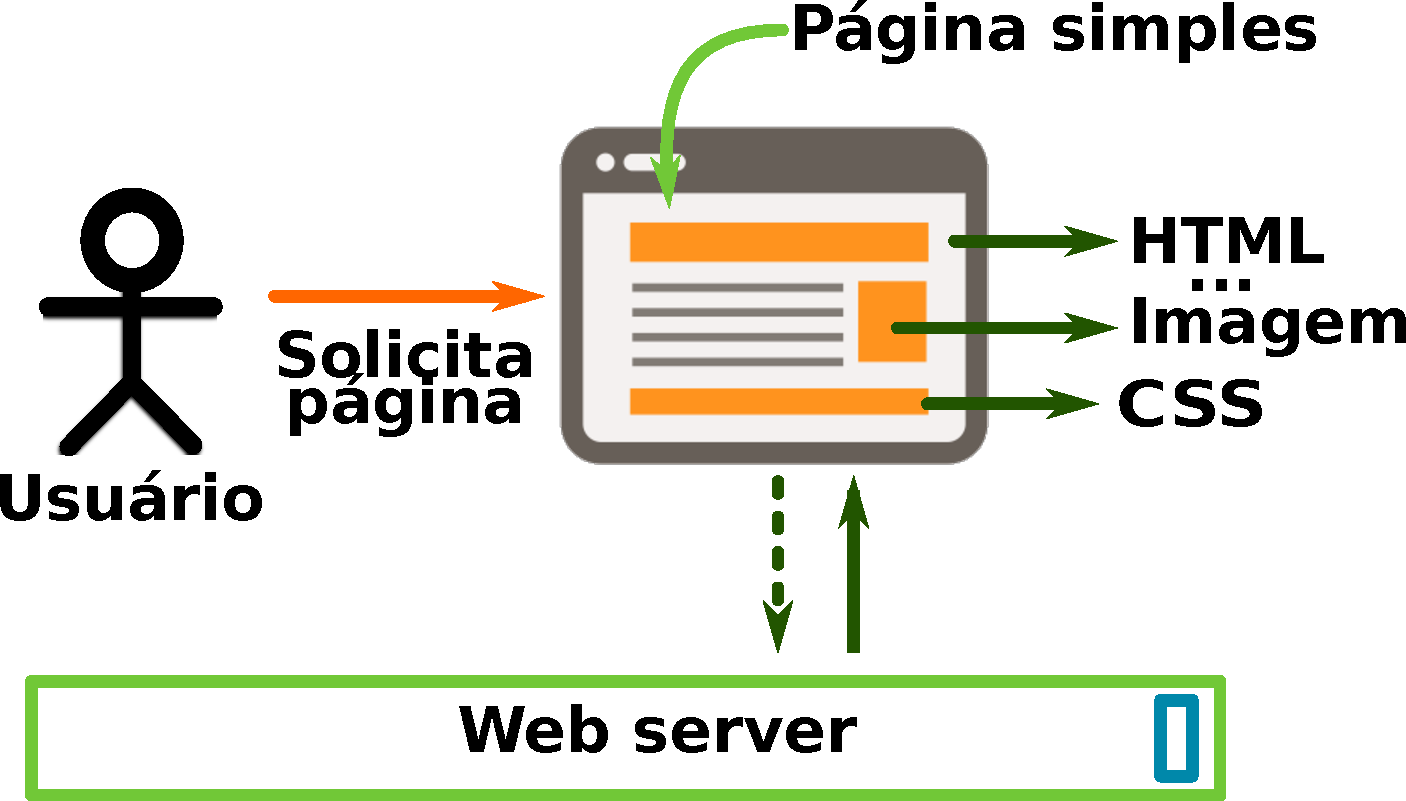
\includegraphics[width=.50\textwidth]{request_a_page}
  \caption{Do cliente para o servidor Web. Note que o navegador solicita em paralelo os damais arquivos necessários para a construção da página}
  \label{fig:client_to_web_server}
\end{figure}

A Figura \ref{fig:client_to_web_server} busca exemplificar uma situação simples
na qual o cliente solicita uma página web para um servidor. Inicialmente, o
cliente faz uma solicitação de alguma página por meio de algum software, vamos
considerar o navegador nesse exemplo. Em seguida, o navegador comunica-se com o
servidor através do protocolo HTTP; por sua vez o servidor responde devolvendo
o arquivo solicitado que contém todas as instruções básicas necessárias para
construir a página (HTML). O navegador abre o arquivo HTML retornado, converte
o conteúdo e verifica se precisa de mais informações para construir a página
solicitada; é comum que a página precise de outros arquivos como CSS, imagens,
javascript, etc. Se mais arquivos forem necessários, então o navegador solicita
os mesmos para o servidor de forma paralela ou serial. O exemplo ilustra de
forma simplificado como uma requisição acontece e como múltiplas requisições
podem ser geradas para construir uma simples tela. Um exemplo real pode ser
considerado da caracterização da carga gerada sobre o site da copa do mundo de
1998, na qual foi gerado uma média de 10796 requisições/min~\citep{worldcup}.
Um servidor web tem que responder milhares de usuários e a estrategia utilizada
para lidar com tal problema são as mais variáveis possível.

Normalmente, cada requisição feita por um cliente abre muitas conexões com o
servidor web e ao final elas são encerradas. Esse mecanismo impacta no
desempenho por duas razões: a latência aumenta e o consumo de CPU com operações
não uteis se eleva. Uma possibilidade para minimizar esses impactos é utilizar
o mecanismo de \boldAndIndex{keep-alive}, que fornece uma conexão
aberta durante as atividades dos usuários. Por exemplo, a Figura
\ref{fig:no_keep_alive} e a Figura \ref{fig:keep_alive} mostram um caso
utilizando \textit{keep-alive} e outra sem utilizar. O primeiro caso ilustra
uma situação padrão na qual uma requisição é realizada, por sua vez são abertas
e fechadas diversas conexões para obter cada um dos arquivos necessários para
construir a página. O segundo caso ilustra uma técnica chamada de
\textit{keep-alive}, cujo o objetivo é reduzir a latência e o uso de CPU no
servidor mantendo a conexão aberta por um intervalo de tempo.  Esse mecanismo
pode melhorar a experiência do usuário ao acessar o site em casos que um
servidor esteja recebendo um elevado número de requisições. Contudo, outro
aspecto do \textit{keep-alive} é que esse pode elevar o consumo de memória
gerando outro tipo de problema em um servidor sobrecarregado.

\begin{figure}[!h]
  \centering
  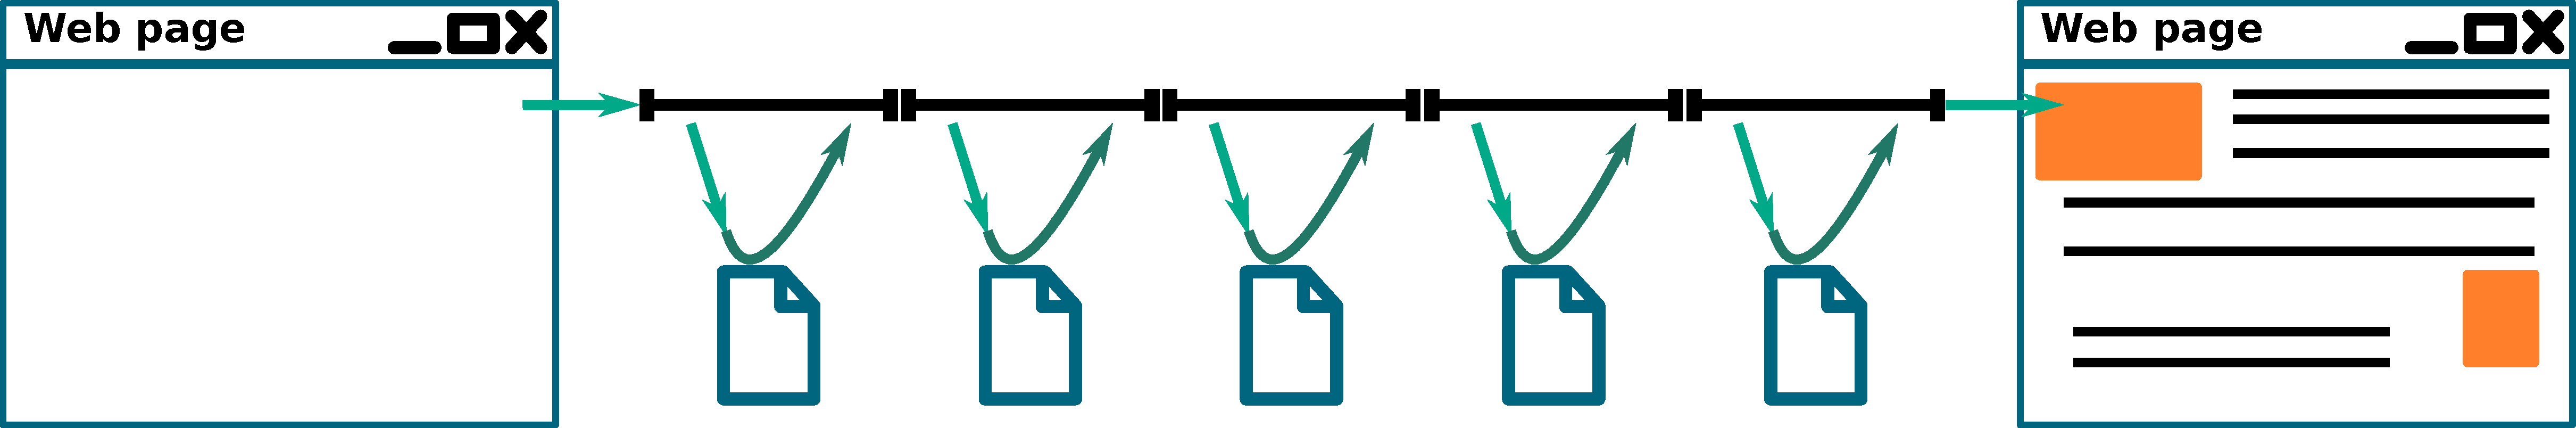
\includegraphics[width=0.8\textwidth]{no_keep_alive}
  \caption{Sem keep alive}
  \label{fig:no_keep_alive}
\end{figure}

\begin{figure}[!h]
  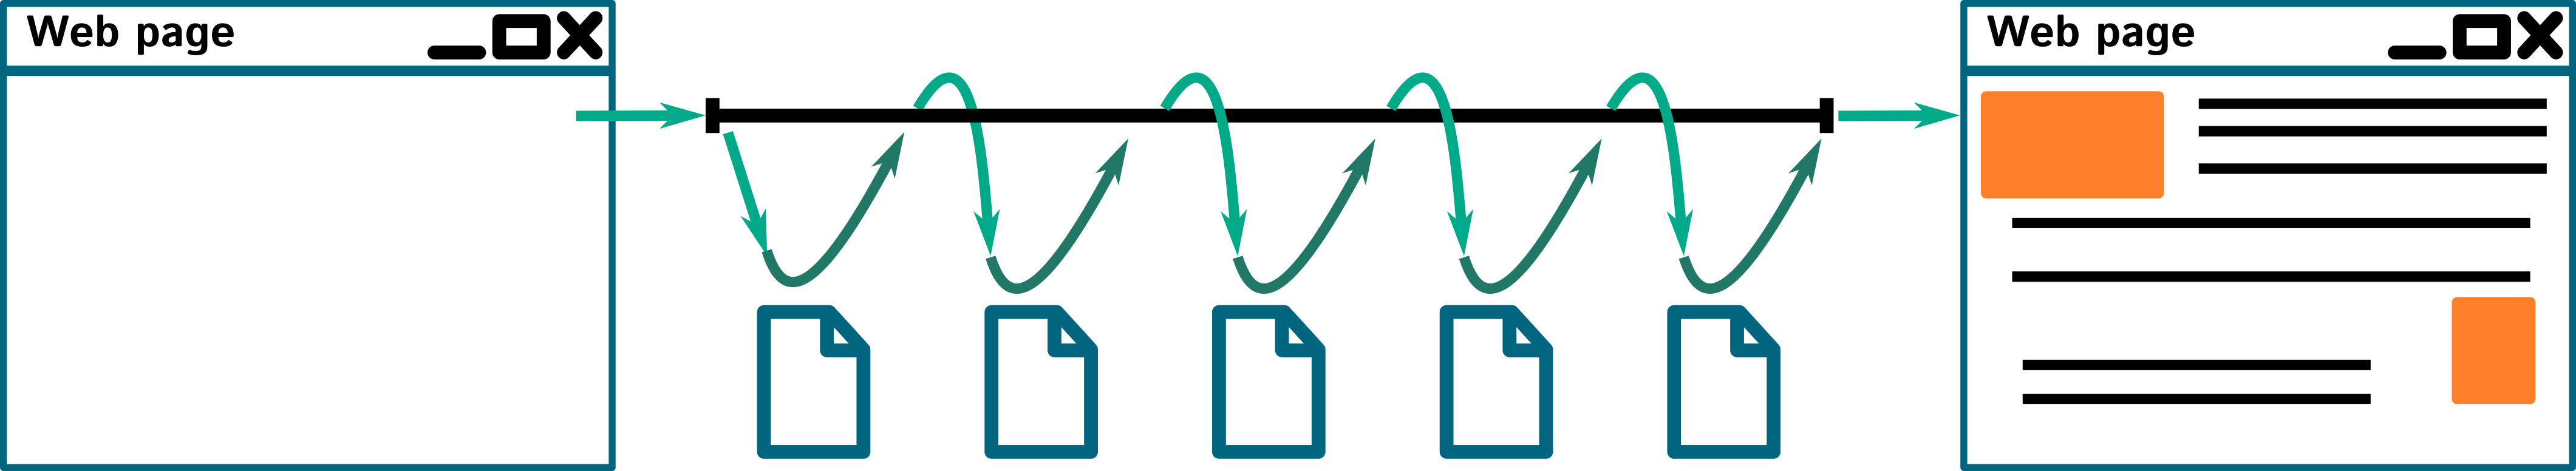
\includegraphics[width=0.8\textwidth]{keep_alive}
  \caption{Com keep alive}
  \label{fig:keep_alive}
\end{figure}

Existem muitos servidores web disponíveis no mercado, contudo, dois deles são
especialmente relevantes para o contexto deste trabalho:
Nginx\footnote{\url{https://www.nginx.com/}} e Apache
Httpd\footnote{\url{https://httpd.apache.org/}}.  O primeiro é conhecido pelo
seu desempenho para entregar arquivos estáticos, enquanto o segundo é conhecido
pela sua enorme estabilidade e comodidade. Ambos são extremamente
configuráveis, confiáveis e suportam grandes cargas de requisições.

\subsection{Servidor Apache HTTPD}
\label{sec:architecture}

O servidor Apache HTTPD, também conhecido como \textit{HTTP Daemon (HTTPD)} é
licenciado com a licença Apache 2.0 e mantido pela fundação Apache.  O Apache
HTTPD\footnote{Usaremos HTTPD e Apache como sinônimos nesse texto} foi
projetado para executar em vários SOs, essa restrição fez com que fosse
necessário adotar estratégias para fazer o HTTPD multiplataforma e mantendo um
bom desempenho.  Uma característica importante do HTTPD é a divisão de módulos
que manipulam processos, threads e bibliotecas portáveis utilizadas; esses
três, em conjunto, constituem a arquitetura do projeto. O Apache utiliza
a biblioteca \textit{Apache Portable Runtime (APR)} cuja a intenção é ser
utilizada como uma interface portável para as tarefas comuns de programação
(e.g.: alocação de memória, manipulação de tempo, etc). Por fim, o HTTPD
implementa um módulo especial chamado \textit{Multi-Processing Module (MPM)}
responsável por manter o processamento das requisições e a lógica de
manipulação de processos/threads. O MPM é uma boa fonte de comparação entre
diferentes modelos de processos.

\begin{figure}[!h]
  \centering
  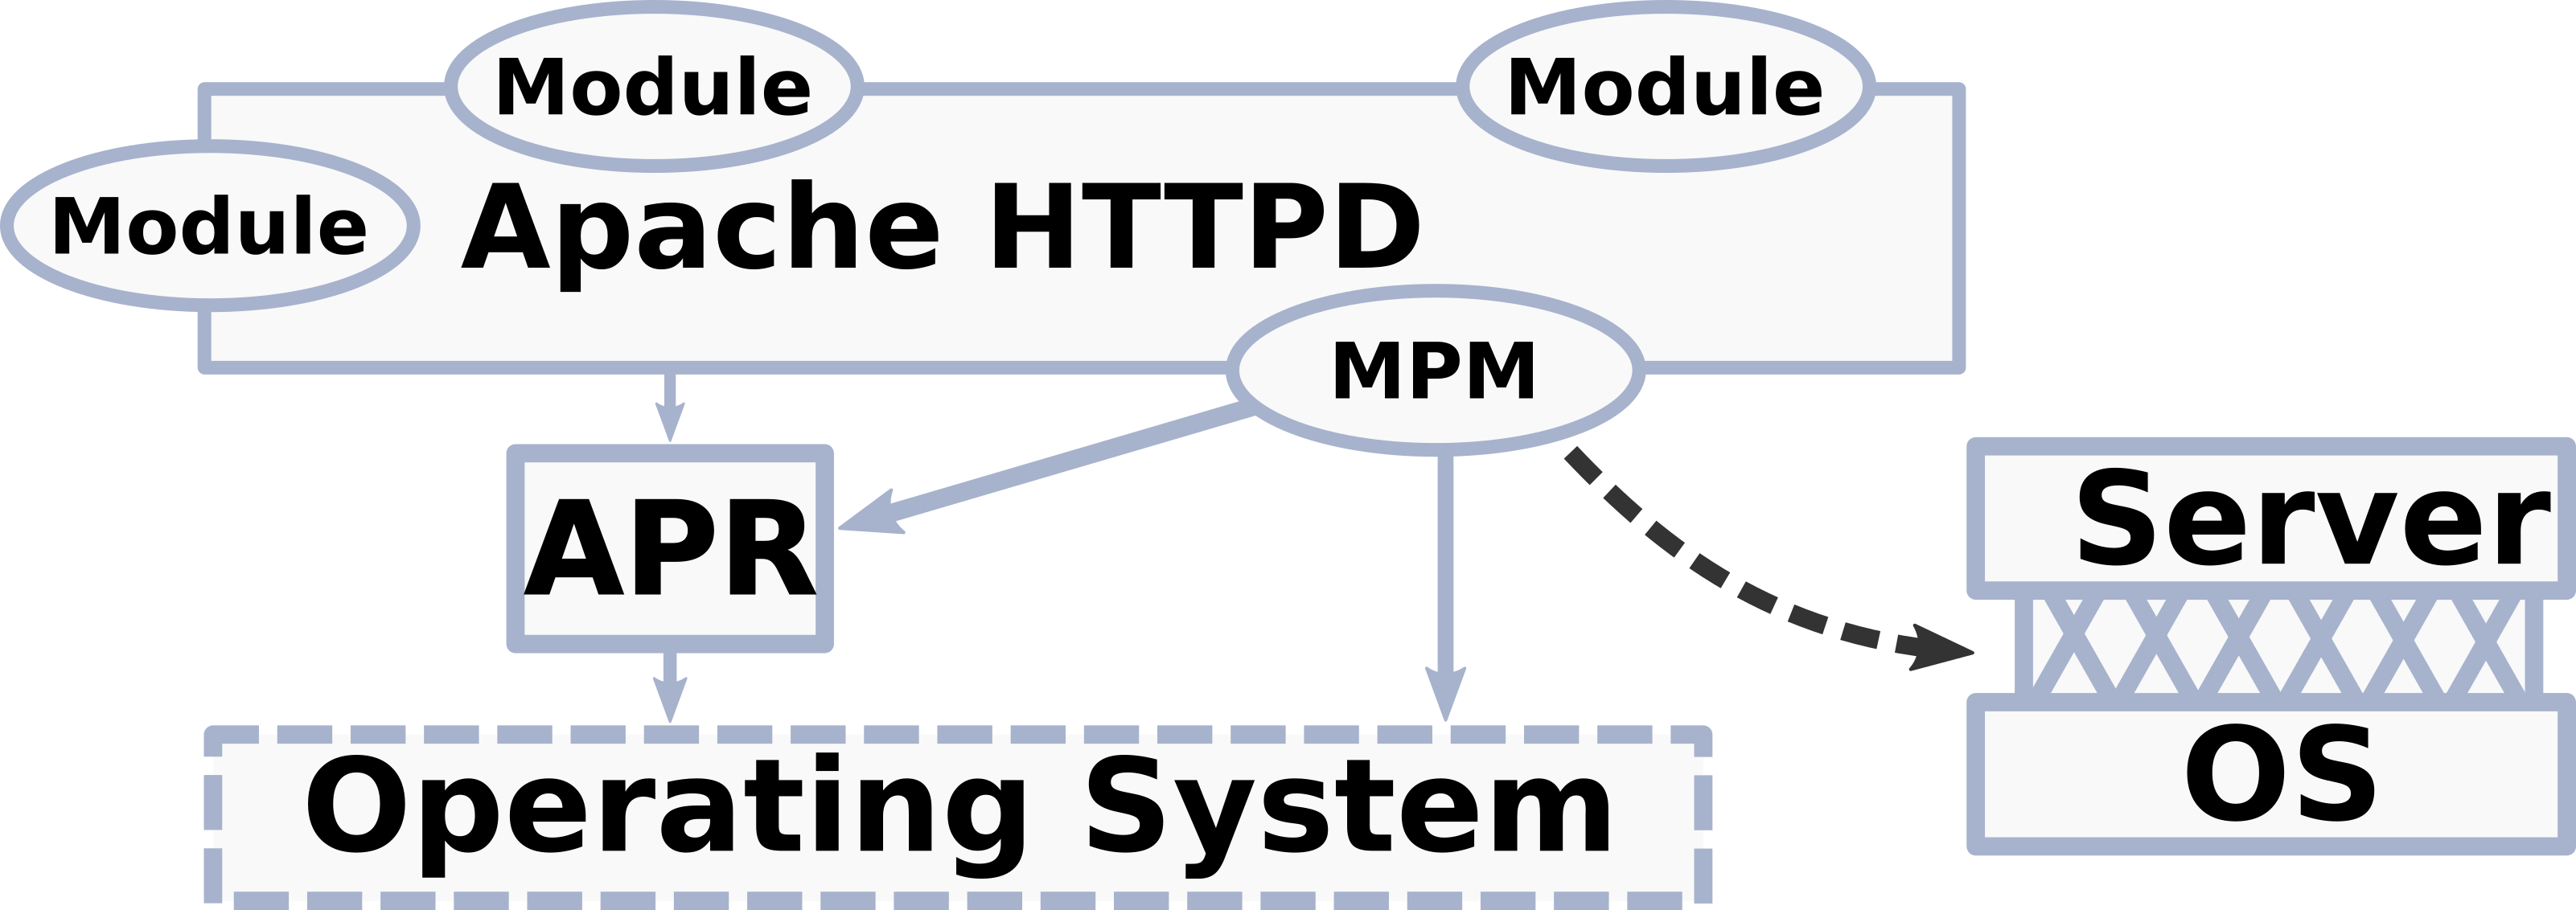
\includegraphics[width=.7\textwidth]{apache_arhitecture} 
  \caption{Arquitetura do servidor Apache HTTP \citep{apache_module_book}}
  \label{fig:apache_architecture} 
\end{figure}

A Figura \ref{fig:apache_architecture} é uma visão de alto nível da arquitetura
do Apache. O topo da imagem representa os elementos do núcleo do Apache
responsáveis por juntar os demais componentes necessários para o seu
funcionamento. Ao redor do núcleo, existe um grande número de módulos anexados
que podem ser conectados ao projeto. Esses módulos facilitam o processo de
adicionar e remover elementos do núcleo, normalmente como bibliotecas
dinâmicas. Módulos na forma de bibliotecas dinamicamente ligadas fornecem
flexibilidade, um bom desempenho e portabilidade entre diferentes SOs (e.g.; o
Window e Linux podem ter diferentes implementações para o mesmo módulo). A
Figura \ref{fig:apache_architecture} também ilustra o MPM como um componente
diretamente conectado ao SO, porque o MPM manipula os elementos de
paralelização e cada SO precisa implementar essa parte de acordo com as suas
próprias particularidades. A última parte da imagem mostra a biblioteca APR,
que se posiciona entre o núcleo do HTTPD e o SO.

\begin{figure}[!h]
  \centering
  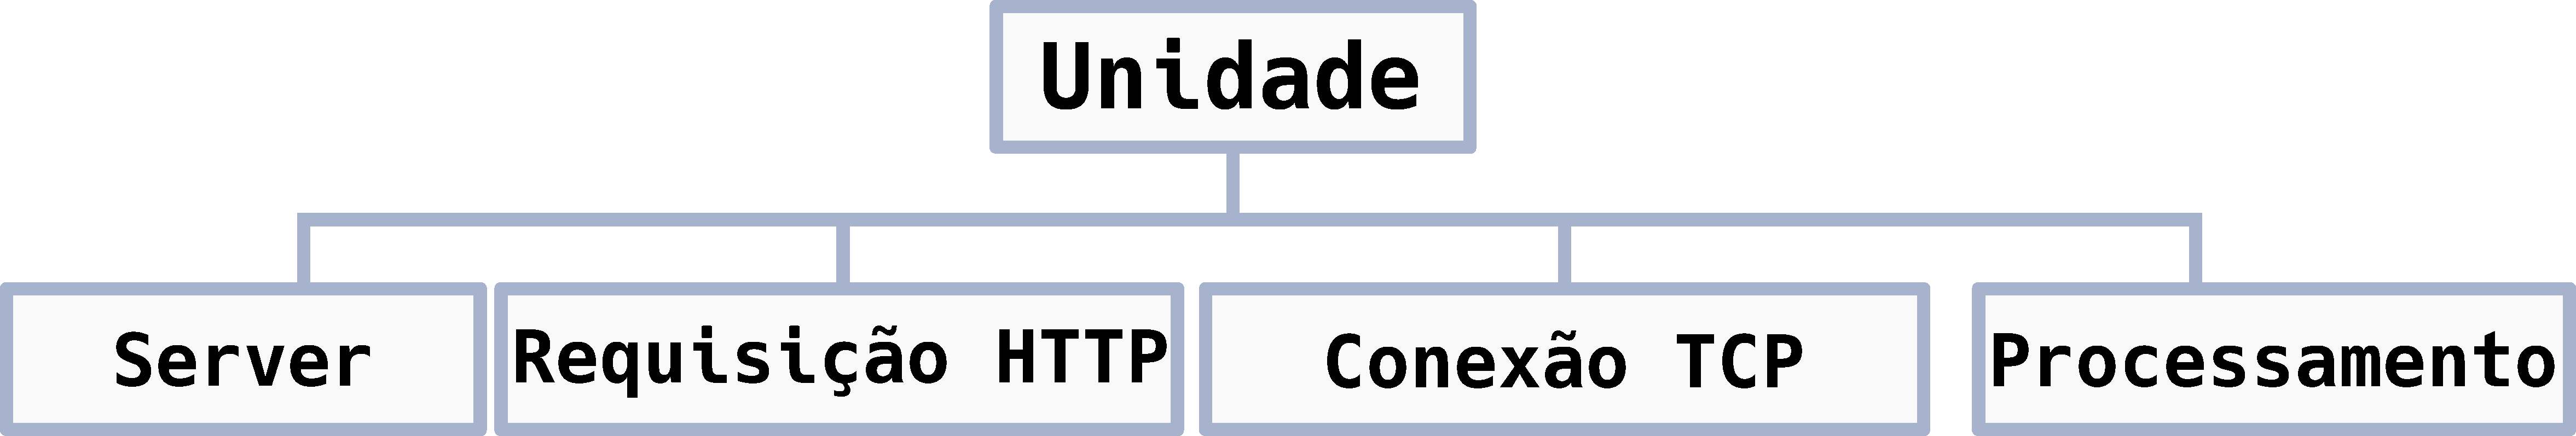
\includegraphics[width=.7\textwidth]{units} 
  \caption{Unidade do Servidor Apache HTTP}
  \label{fig:units} 
\end{figure}

Alguns módulos são essenciais para o funcionamento do HTTPD uma vez que eles
representam os elementos básicos das estruturas de dados que são usadas por
todo o código. A Figura \ref{fig:units} mostra algumas unidade fundamentais
usadas pelo HTTPD. O módulo \textit{server} é responsável por criar uma estrutura de
dados para a requisição toda vez que o HTTPD aceita uma nova conexão. O módulo
HTTP é encarregado de preencher uma estrutura de dados de requisição e o
módulo de conexão TCP constrói a estrutura de dados que mantém as informações
da conexão. Normalmente, não é preciso se preocupar com módulos relacionados
aos detalhes do HTTP, uma vez que o Apache ajusta todos os elementos necessários
e também entrega uma estrutura de dados pronta para ser utilizadas.

\begin{figure}[!h]
  \centering
  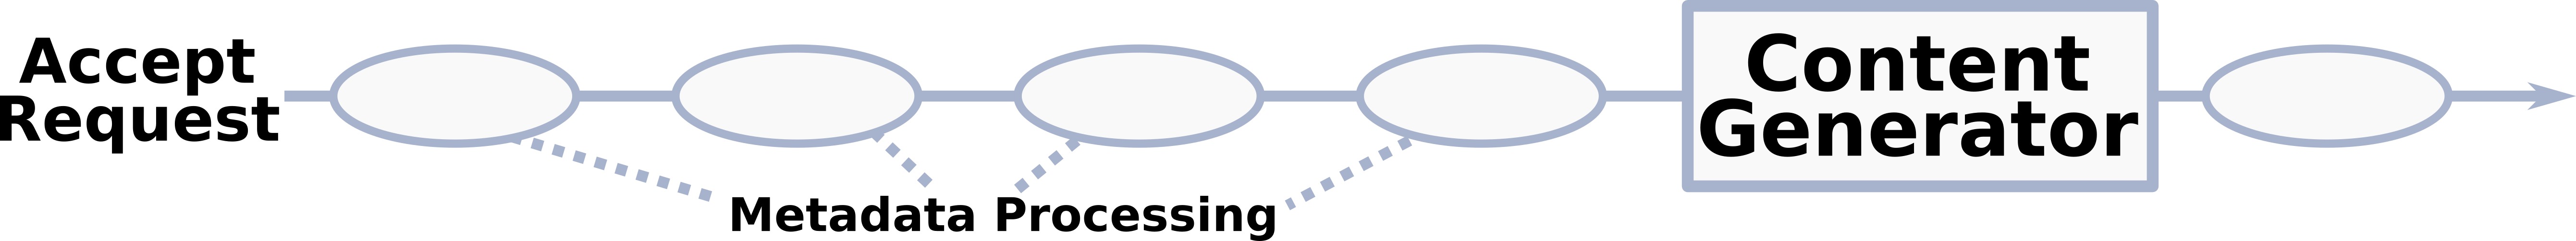
\includegraphics[width=.9\textwidth]{request_phases} 
  \caption{Gerador de Conteúdo \citep{apache_module_book}}
  \label{fig:content_generator} 
\end{figure}

Outros dois aspectos da arquitetura do Apache são o \textbf{Content Generator}
(Gerador de Conteúdo) e as fases de processamento das requisições. O
\textit{Content Generator} pode ser visto como o núcleo do Apache uma vez que
ele é responsável pelas operação de escutar por requisições e retornar
respostas; existe exatamente um gerador de conteúdo por requisição. No Apache
um módulo pode registrar um \textit{content generator} de forma simples (basta
ajustar o \texttt{httpd.conf}) e se nenhum estiver disponível o Apache utiliza
o gerador padrão que simplesmente mapeia um arquivo para uma requisição
\citep{apache_module_book}. O \textit{content generator} pode processar toda a
requisição sozinho, contudo o Apache divide a \textit{request} em várias fases
como pode ser visto na Figura \ref{fig:content_generator}. Alterações nessa
fases podem ser extremamente proveitosas para testar novas abstrações de
processos.

\subsubsection{MPM}
\label{sec:prefork}

O módulo \textit{Multi-Processing (MPM)} é um elemento especial dentro do
Apache. Como a Seção \ref{sec:architecture} introduziu, o MPM funciona como uma
interface entre o HTTPD e o SO. O MPM tem três características principais para
qualquer instância do Apache: deve ser único, é obrigatório e tem uma
implementação específica para o SO alvo. O HTTPD fornece pelo menos um módulo
MPM por SO, por exemplo, o Window utiliza \texttt{mpm\_winnt} e o Linux tem
três opções diferentes que serão tratadas em detalhes nesse trabalho. Cada uma
das três opções podem ser classificadas como baseada em processos ou em
threads, mais especificamente são elas: \textit{Prefork}, \textit{Worker} e
\textit{Event}. Esses módulos constituem bons pontos para comparar thread e
processos usando as novas abstrações, uma vez que o ambiente se conserva.

\begin{description}

	\item[Prefork:]

O \textit{Prefork} foi a primeira estratégia adotada pelo HTTPD e é totalmente
baseada em processos. A Figura \ref{fig:prefork} ilustra os três passos
realizados pelo \textit{Prefork}. O Apache inicia com um processo responsável
por gerir os filhos que serão encarregados de manipular uma requisição por vez.
Em seguida, ao receber uma requisição, o processo de controle identifica um
processo que esteja sem fazer nada e repassa a mesma para um processo filho que
se encarrega da tarefa de manipular a solicitação. Caso não exista nenhum
processo filho disponível para manipular a requisição, então o processo de
controle cria novos processos filhos. Repare que a processo de controle
comporta-se como um \textit{load balancing}.

\begin{figure}[!h]
  \centering
  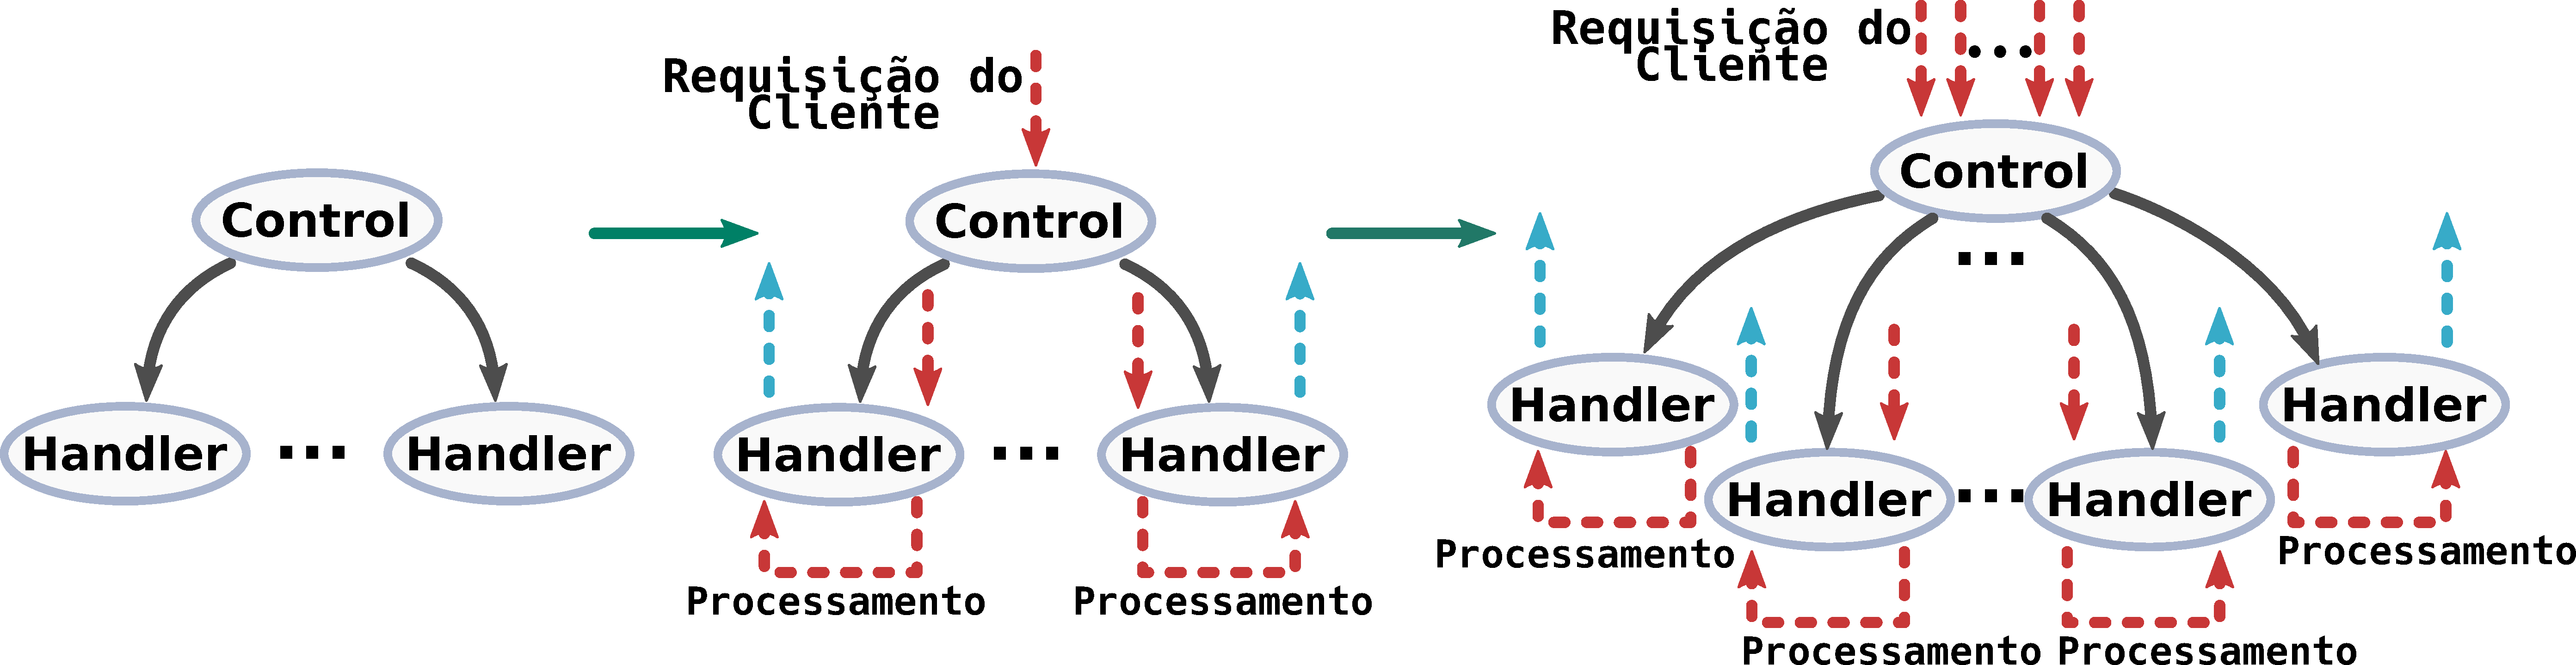
\includegraphics[width=\textwidth]{prefork} 
  \caption{Prefork}
  \label{fig:prefork} 
\end{figure}

O \textit{Prefork} é uma boa opção para servidores web que não são compatíveis
com threads (e.g., aplicações legadas escritas em PHP) e é a melhor opção de MPM
para isolar uma única requisição. Contudo, o \textit{Prefork} consome muita
memória e CPU o que não é desejável em um servidor sob forte demanda.

	\item [Worker]: O \textit{Worker} é uma solução híbrida uma vez que o seu design é baseado em
processos e threads. Esse módulo tem um processo de controle que é responsável
por criar um processos filhos e controlar o balanceamento da carga entre os
filhos. Ao contrário do \textit{Prefork}, o \textit{Worker} não cria instâncias
de processos filhos para manipular requisições feitas pelos clientes. Ele cria
diversos processos novos na qual cada um possuí várias threads para realizar a
tarefa de tratamento das requisições; comumente, o HTTPD tem que manipular uma
grande carga de requisições e nesses casos o processo de controle age criando
novos filhos (cada um com um conjunto de threads) para suportar a carga.
Repare que o \textit{Worker} utiliza threads para manipular as requisições,
isso faz com que o total de processos filhos criado seja relativamente pequeno
(comparado com o \textit{Prefork}) e consequentemente o consumo de memória
reduz. O HTTPD tem um arquivo de configuração que permite um controle fino de
todos os parâmetros relacionados ao número máximo de processos filhos, o total
de threads por filhos, o número de reposição de processos filhos e threads,
dentre outros.

\begin{figure}[!h]
  \centering
  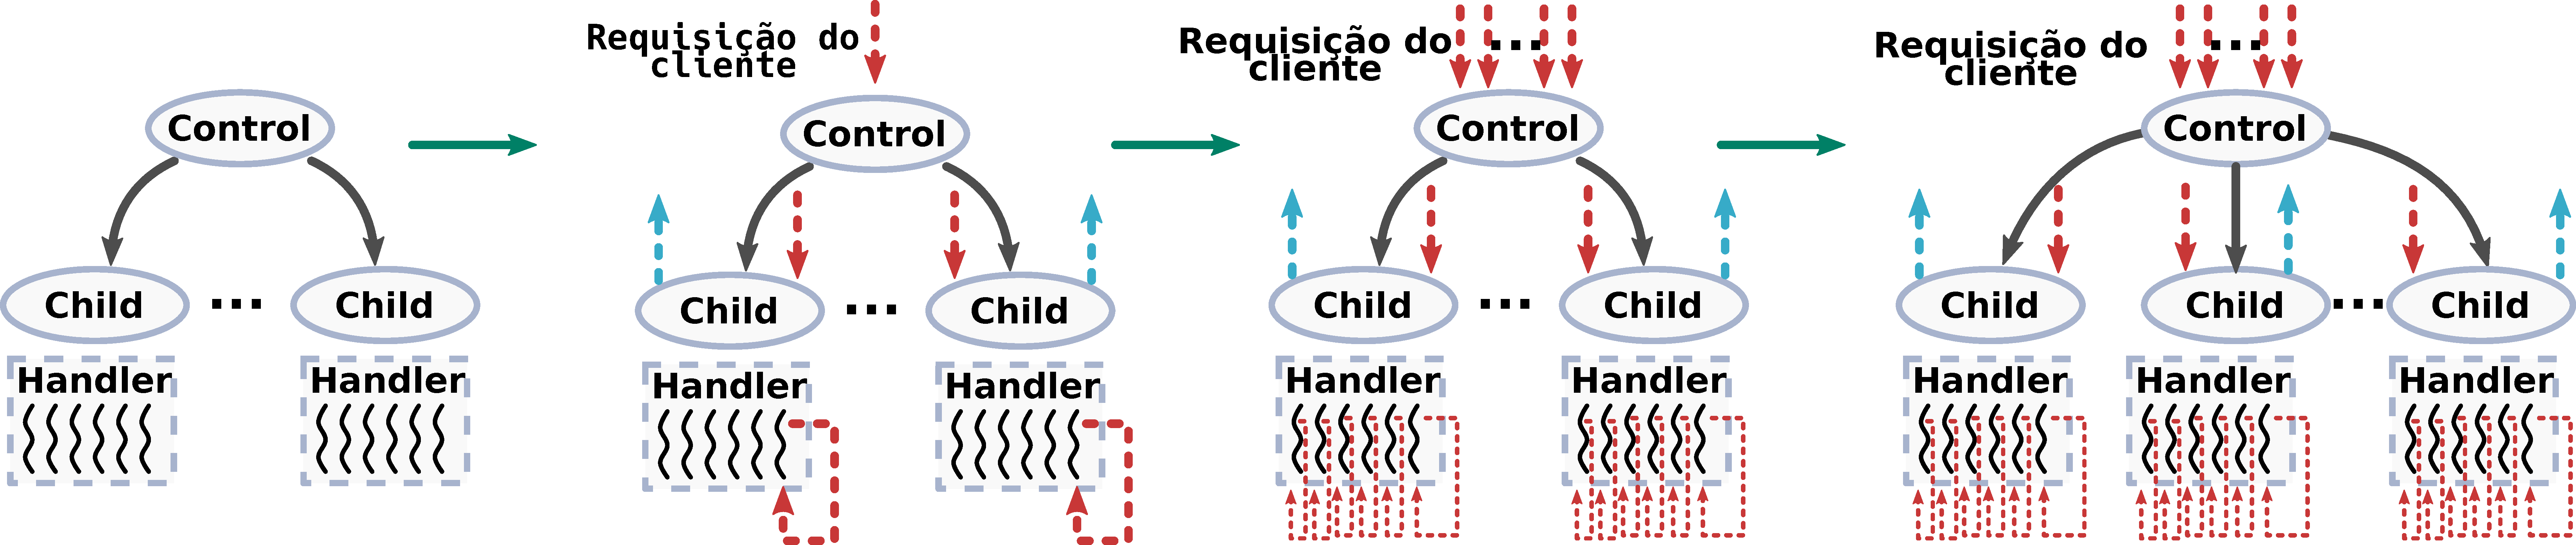
\includegraphics[width=\textwidth]{worker} 
  \caption{Worker}
  \label{fig:worker} 
\end{figure}

A Figura \ref{fig:worker} é um exemplo de como o \textit{Worker} funciona.
Quando o Apache inicia, ele tem um processo de controle e alguns processos
filhos que mantém um grupo de threads paradas. A segunda parte da figura
representa o caso em que o HTTPD recebe um grande número de requisições e o
processo de controle cria mais filhos para suportar a carga. O \textit{Worker}
consome menos memória que o \textit{Prefork} e consequentemente ele é melhor em
casos no qual o servidor está sobrecarregado.  A mistura de processo e thread
adiciona estabilidade para todo o sistema.

	\item [Event:] O módulo \textit{Event} é baseado em threads e é o padrão na
última versão do Apache. O comportamento básico do \textit{Event} é similar ao
do \textit{Worker} com duas características a mais: \textit{keep-alive} e
separação de responsabilidade de enviar dados para o cliente. A Figura
\ref{fig:event} ilustra o comportamento básico do \textit{Event}. A forma na
qual o \textit{event} opera é similar ao \textit{worker}, com a diferença de
que ele cria um processo a mais só para manipular o envio dos dados para o
cliente.

\begin{figure}[!h]
  \centering
  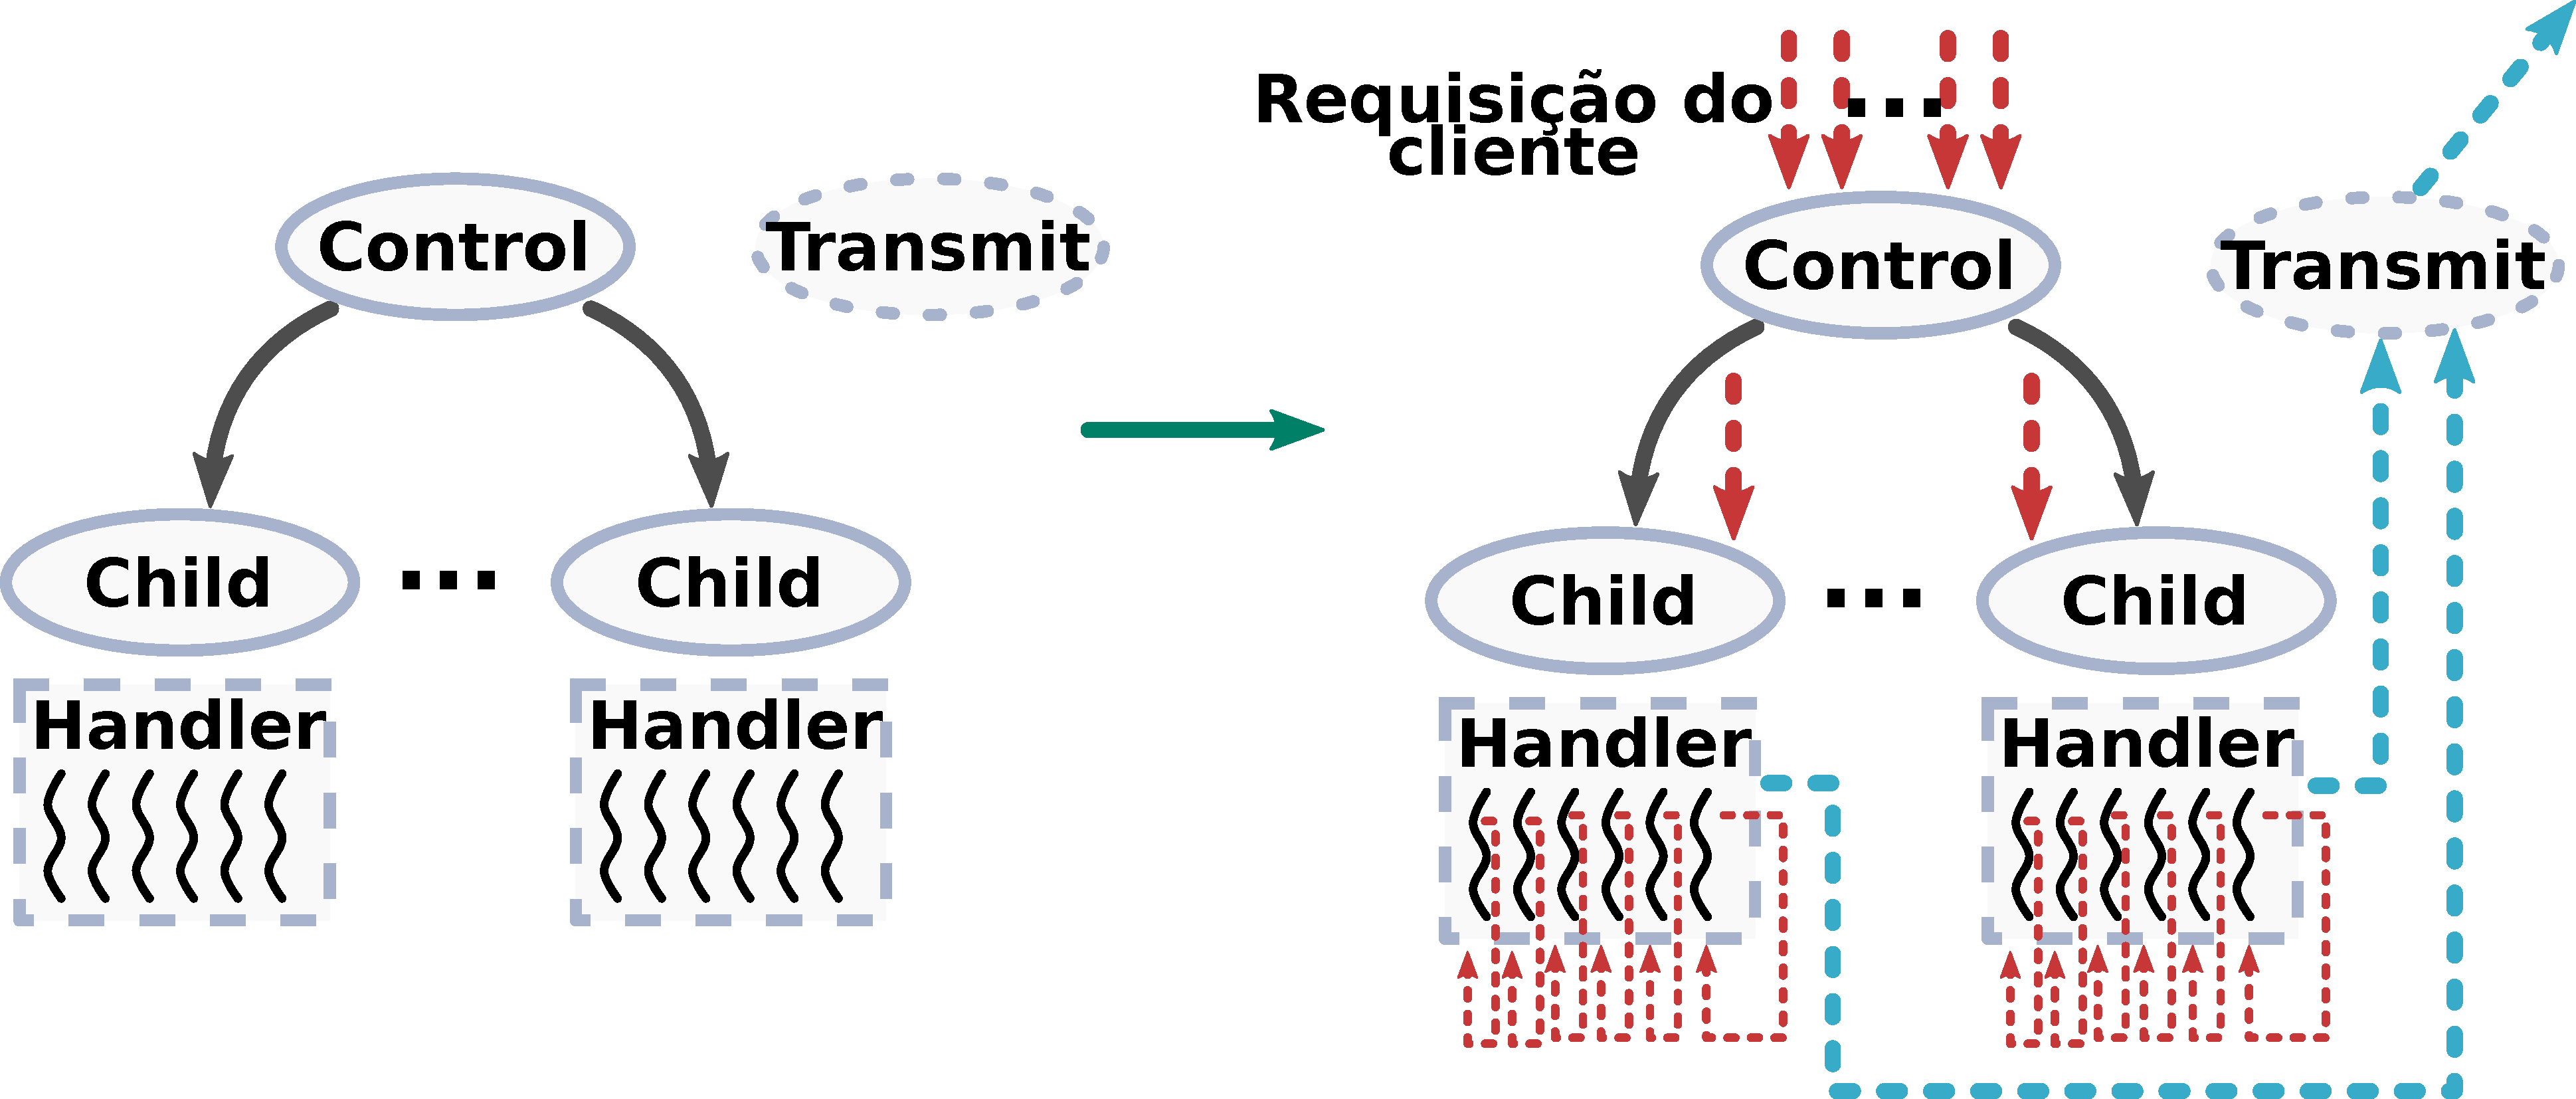
\includegraphics[width=.7\textwidth]{event} 
  \caption{Event}
  \label{fig:event} 
\end{figure}

\end{description}

\subsection{Nginx}

Assim como o Apache HTTPD o Nginx é um servidor web, contudo esse diferencia-se
de muitas formas dos servidores web tradicionais. A sua principal
característica é o seu excelente desempenho para atender requisições,
principalmente aquelas relacionadas a arquivos estáticos. Além disso o Nginx
comporta-se como um \textit{reverse-proxy}; ele recebe uma requisição do
usuário, por sua vez ele repassa a requisição para uma aplicação especifica
responsável por realizar o processamento (e.g. Puma, PHP-FPM, etc). Quando o
dado é processado pela aplicação, essa retorna o resultado para o Nginx que
repassa os dados para o usuário \citep{soni}. A Figura \ref{fig:nginx_basico}
ilustra o funcionamento geral do Nginx, note que a requisição do usuário chega
ao servidor encriptada por meio do protocolo SSL (apresentamos esse protocolo
na Seção \ref{sec:openssl}), em seguida o Nginx trata a solicitação
transformando ela em HTTP; por fim, o processo termina repassando a request
para algum serviço manipular.

\begin{figure}[!h]
  \centering
  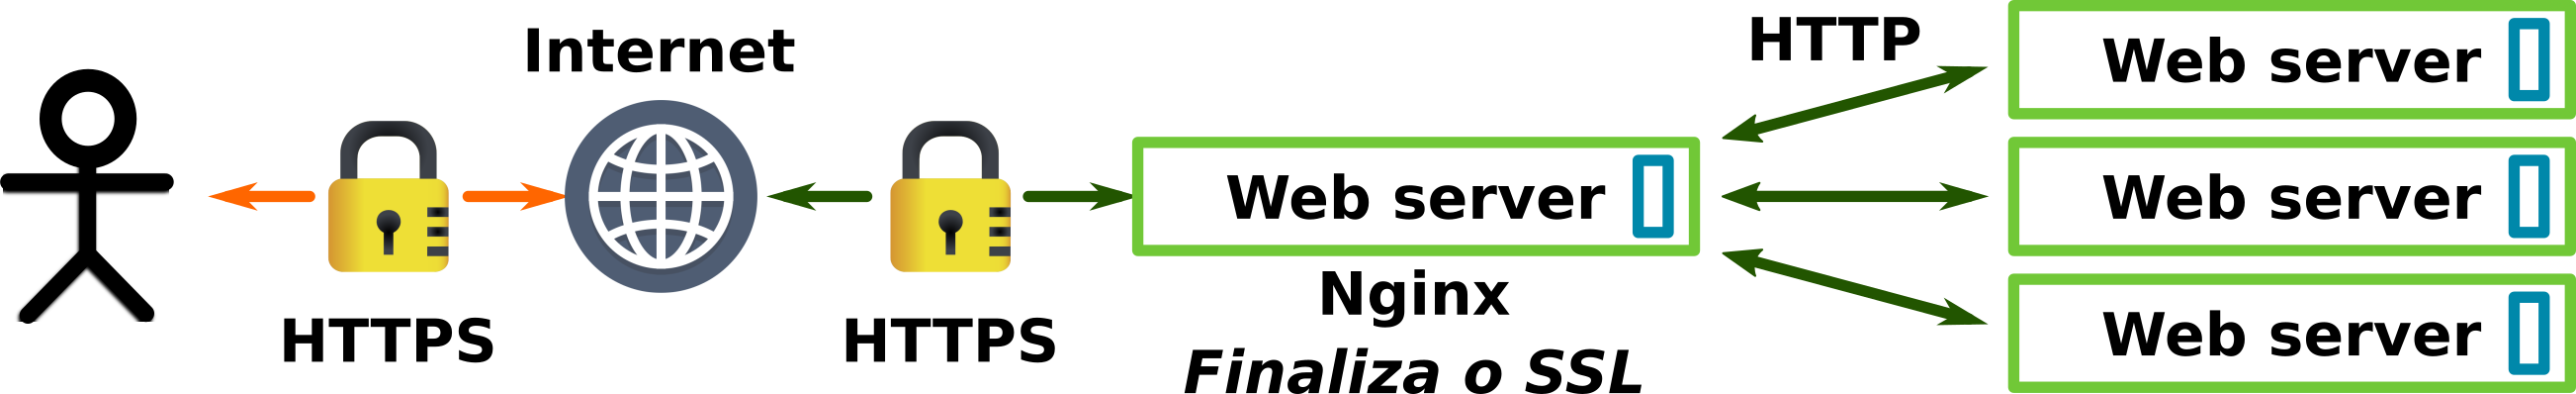
\includegraphics[width=\textwidth]{nginx_load_balancer_ex} 
  \caption{Nginx comportando-se como reverse-proxy \citep{soni}}
  \label{fig:nginx_basico} 
\end{figure}

A grande maioria dos servidores web buscam tirar o máximo de proveito dos recursos
de hardware utilizando um elevado número de threads e processos. Essa abordagem
é relativamente simples de se implementada e traz bons resultados, contudo ela
também tem alguns problemas. Dentre as desvantagens, temos que o modelo baseado
em threads/processos geram uma grande quantidade de operações que bloqueiam e
consequentemente geram trocas de contexto. Além disto, a abordagem baseada em
threads/processos consome uma elevada quantidade de recursos degradando o
desempenho da aplicação em situações de elevada demanda.

O Nginx sugere uma abordagem nova de servidor web baseada na ideia de eventos.
A estratégia de eventos parte do princípio que deve-se evitar ao máximo a troca
de contexto e assim tirar o máximo de proveito da CPU com processamento útil.
Por esse motivo o Nginx cria apenas três tipos de processos
\citep{nginx_architecture}:

\begin{itemize}
  \item Processo mestre, faz operações privilégiadas como ler arquivos de configuração e acessar portas;
  \item Processo de cache de disco, carrega dados do disco fazendo cache na memória;
  \item Processo que gerencia o cache e que realiza verificações sobre o cache periodicamente;
  \item Processos \textit{Worker} são os processos que fazem o trabalho de manipular conexões, ler e escrever em disco e comunicar-se com os servidores.
\end{itemize}

O Nginx recomenda um \textit{Worker} por núcleo da CPU, isso permite tirar
grande proveito dos eventos.

Na prática o sistema de eventos é eficiente pois gera poucos bloqueios
(comparado com o modelo que utiliza threads/processos) uma vez que esse não
espera a aplicação terminar o que está fazendo. Por exemplo, se o
\textit{worker} estiver atendendo uma requisição e em um determinado momento
precisar recuperar uma informação do disco, o \textit{worker} não bloqueia, ele
simplesmente vai fazer outra tarefa e salva o evento referente a busca no disco
para retornar nele depois (mais precisamente, quando surgir um evento). O
sistema de eventos faz com que um único \textit{worker} execute múltiplas
tarefas de forma sequencial sem bloqueio e consequentemente com poucas trocas
de contexto.

\section{Ferramentas de Comunicação Encriptada}
\label{sec:com_enc}

Como mostrado no Capítulo \ref{cap:trabalhos-analisados}, algumas das novas
propostas de abstrações de processos levam melhorias de segurança para o espaço
de usuário. Nesse sentido aplicações que envolvem mecanismos de encriptação ou
que buscam levar algum nível de segurança, representam bons casos de uso para
validar novas abstrações. Esse tipo de software costuma ser desenvolvido por
uma comunidade de especialistas na área de segurança, o que significa que levar
melhorias nesse tipo de ferramenta não é uma tarefa trivial. Essas
características fazem com que esse tipo de aplicação representem bons caso de
validação para novas abstrações de processos. Por uma questão de simplicidade e
abrangência escolhemos duas ferramentas amplamente utilidades: OpenSSH e
OpenSSL.

\subsection{OpenSSL}
\label{sec:openssl}

Antes de discutir sobre o OpenSSL é importante apresentar de forma geral o
protocolo \boldAndIndex{Secure Sockets Layers (SSL)}. O principal objetivo do
SSL é fornecer um conjunto de protocolos criptográficos que permita a
comunicação segura na rede. Basicamente, esse constituí uma ferramenta de uso
cotidiano, tendo diversas aplicações de missão crítica dependendo de tal
protocolo o que faz dele um constante alvo de ataques.

O SSL utiliza um mecanismo chamado de \boldAndIndex{handshake} que
nada mais é do que um processo de negociação entre o cliente e o servidor de
forma a criar uma conexão segura entre ambos, a Figura
\ref{fig:openssl_handshake} descrever de forma geral os passos da negociação. O
processo de \textit{handshake} começa com o cliente mandando uma mensagem do
tipo "Oi, sou o cliente" para o servidor; nessa mensagem o cliente informa a
versão do SSL que está usando, os algoritmos de criptografia e os métodos de
compressão que ele sabe manipular. O servidor por sua vez manda um "Oi, sou o
servidor" dizendo qual algoritmo usar (selecionado da lista que o cliente
mandou), um ID da seção, um certificado digital e a sua chave pública. Com o
certificado, o cliente consulta uma \textit{Certificate Authority (CA)}
(Autoridade Certificadora) que valida se o servidor é valido ou não, isso serve
para estabelecer a confiança sobre o servidor. Depois que o cliente recebe a
validação da CA, ele começa a etapa de troca de chaves na qual o cliente envia
a chave secreta compartilhável. O cliente criptografa tal chave com a chave
pública fornecida pelo servidor e o cliente termina enviando uma mensagem de
fim. O servidor desencripta a mensagem do cliente e utiliza a chave enviada
para criptografar uma mensagem de fim para ser enviada para o o cliente. Quando
o \textit{handshake} termina, o servidor e o cliente podem enviar mensagens que
são simetricamente encriptadas \citep{openssl}.

\begin{figure}[!h]
  \centering
  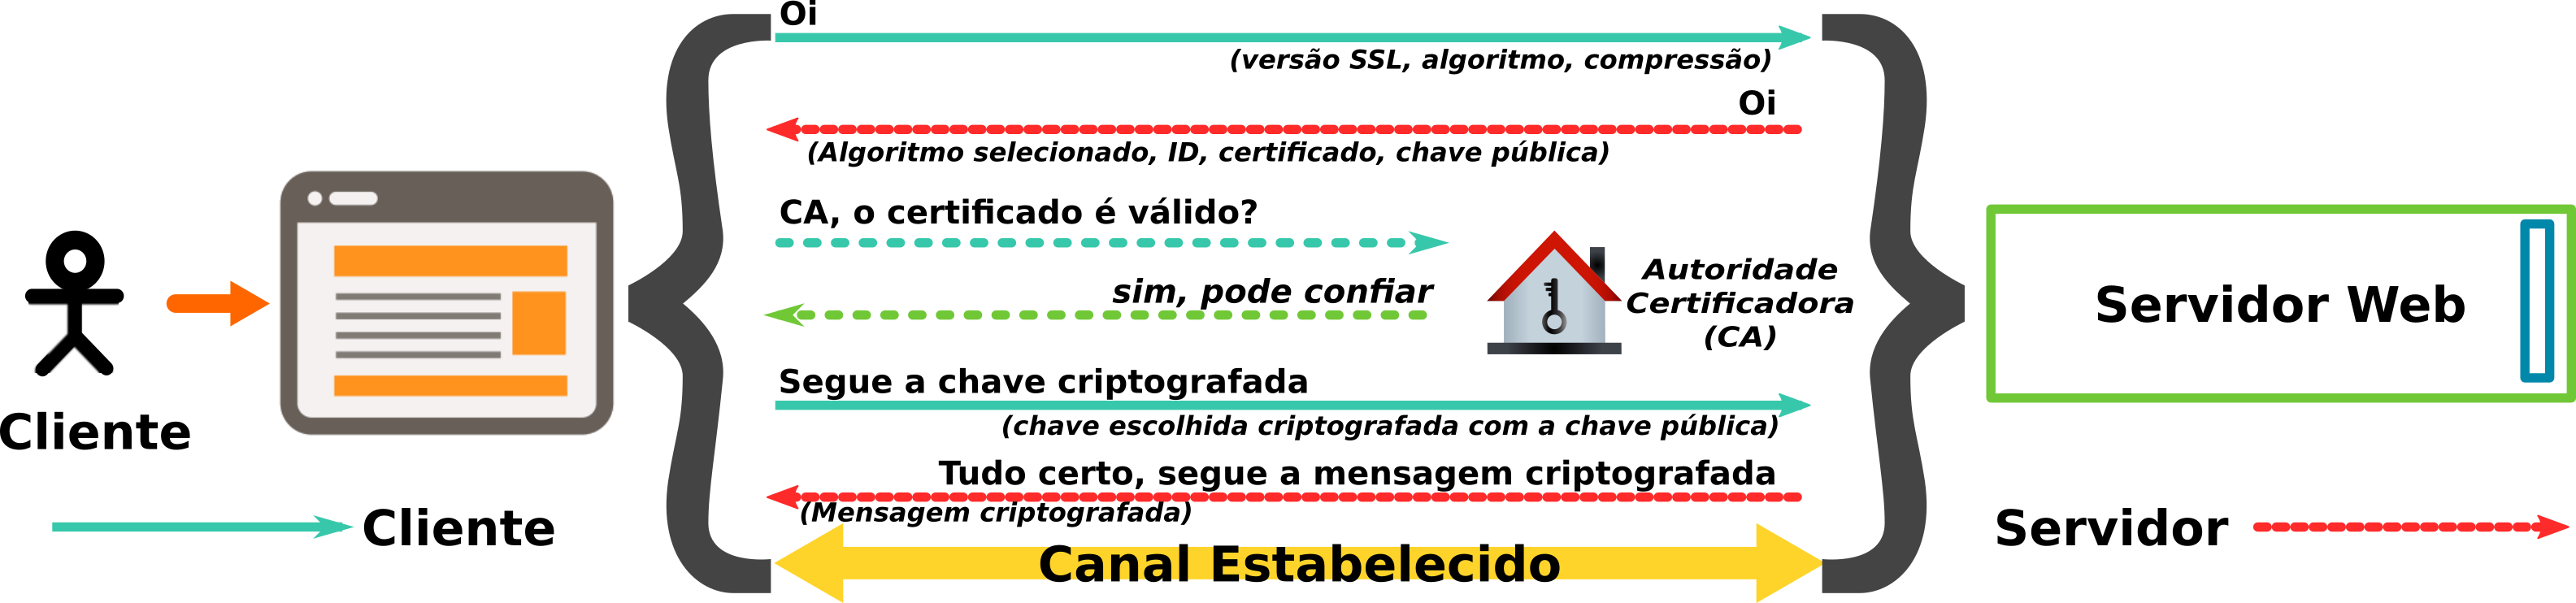
\includegraphics[width=\textwidth]{ssl_handshake}
  \caption{Do cliente para o servidor Web}
  \label{fig:openssl_handshake}
\end{figure}

O OpenSSL é uma implementação livre do protocolo SSL, ele contém a
implementação de várias funções criptográficas e utilitárias. A Figura
\ref{fig:openssl_arch} mostra uma visão geral da arquitetura do OpenSSL. O
\textit{EVP crypto API} são funções de alto nível que fornecem recursos para
derivação de chaves, hash seguro, código de autenticação de mensagens,
encriptação/decriptação de algoritmos simétricos/assimétricos, dentre outros. A
arquitetura também fornece uma pilha de manipulação de erros e uma interface
abstrata para lidar com I/O.

\begin{figure}[!h]
  \centering
  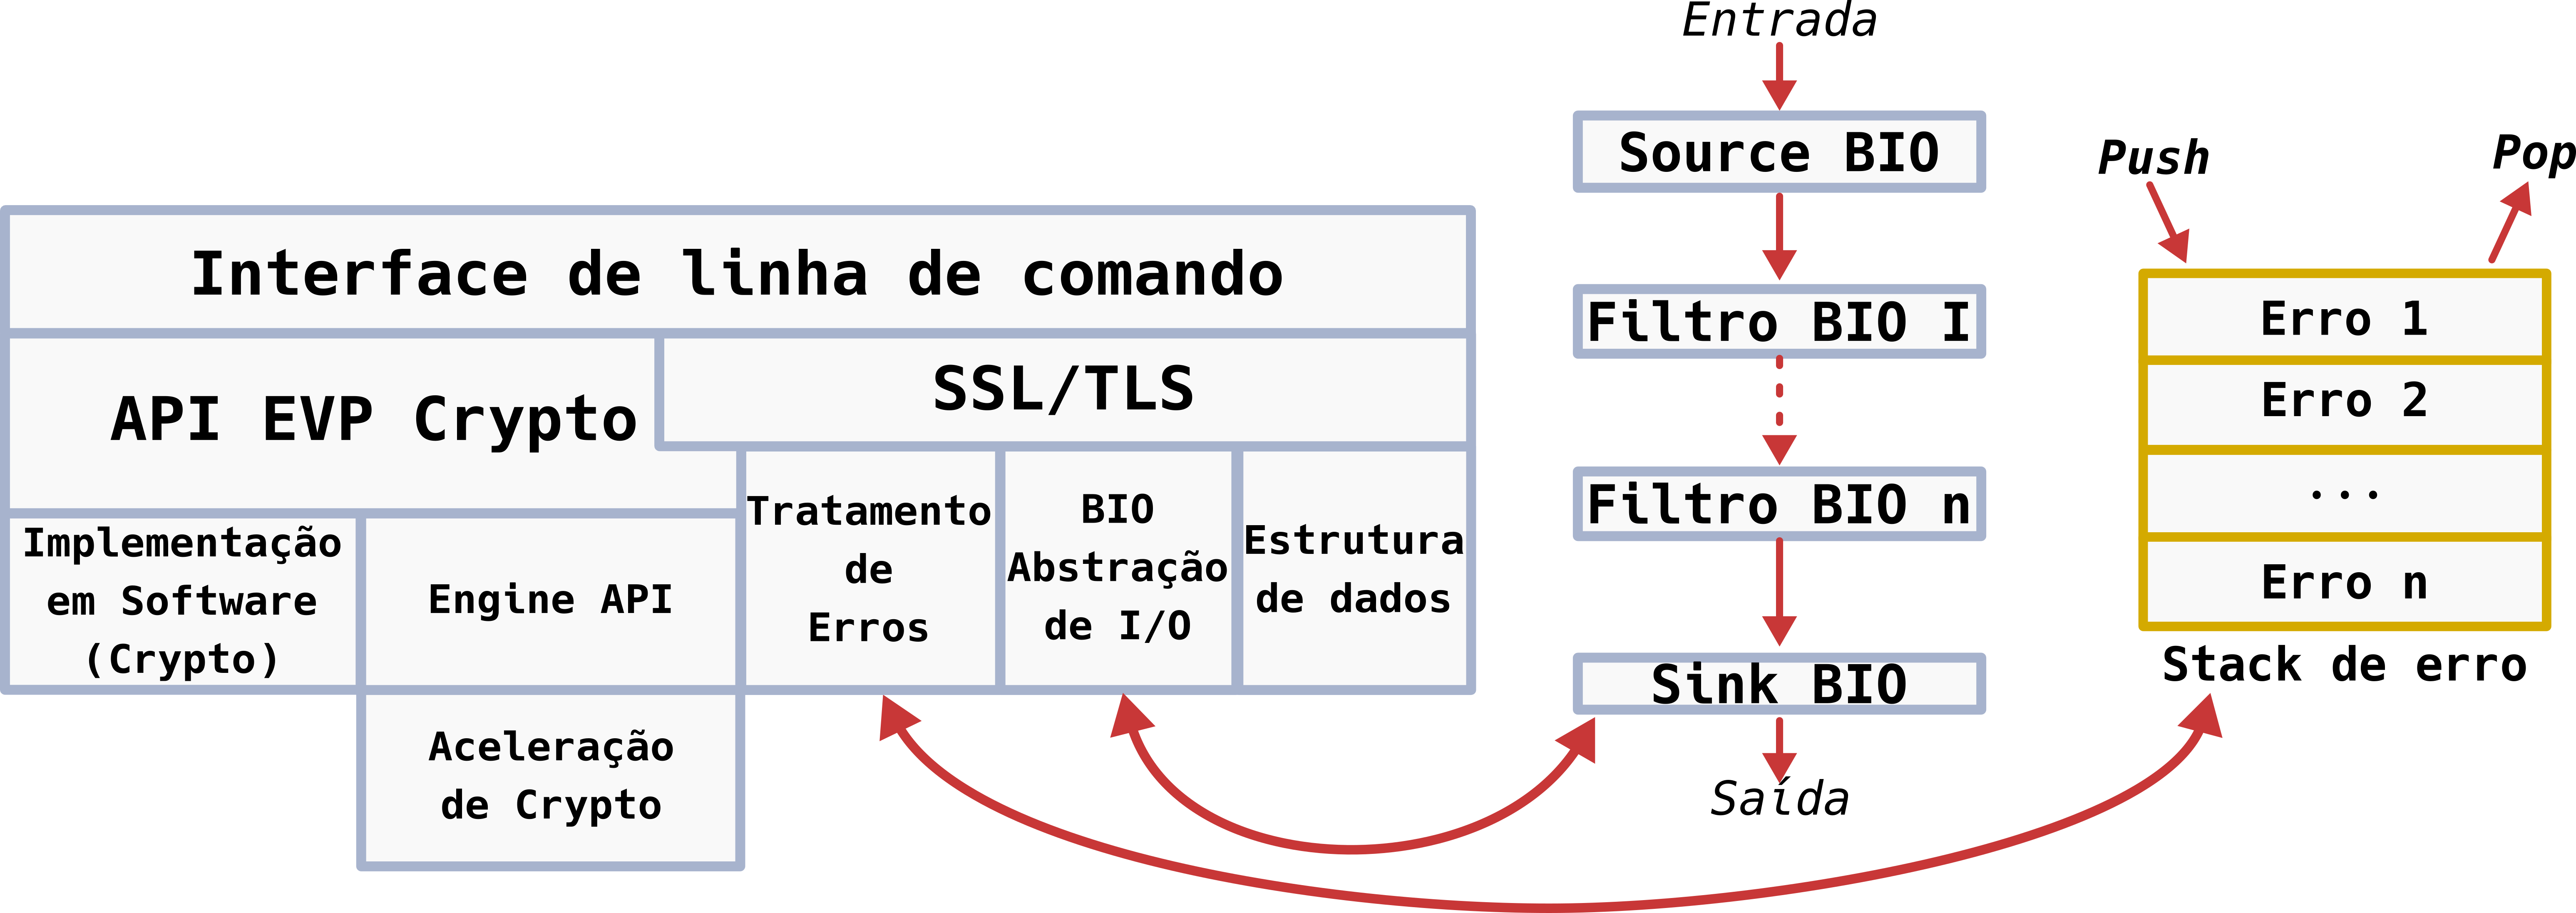
\includegraphics[width=\textwidth]{openssl_arch}
  \caption{Arquitetura do OpenSSL \citep{crypto_openssl}}
  \label{fig:openssl_arch}
\end{figure}

\subsection{OpenSSH}

Uma das tarefas mais comuns do dia-a-dia de muitos desenvolvedores consiste em
acessar servidores em diversos locais do mundo e configurar uma determinada
aplicação. Na prática, boa parte dos profissionais de TI faz uso de conexões
seguras na Internet por meio do protocolo \textit{Secure Shell (SSH)}. Existem
diversas implementações desse protocolo, mas para este trabalho discutiremos o
OpenSSH.

A Figura \ref{fig:openssh_layer} apresenta uma visão geral da arquitetura do
OpenSSH. Primeiramente repare que as três camadas correspondentes as camadas
SSH encontram-se sobre a camada TCP/IP que consistem em uma conexão não segura.
A primeira camada se chama \textit{ssh-transport} e ela é responsável por
realizar operações criptográficas, proteção contra ataques e reverificar chaves
de tempos em tempos. Logo após a primeira camada temos o \textit{ssh-userauth}
que é responsável pela autenticação, se tudo der certo durante a autenticação,
então a troca de chaves acontece e a conexão segura é estabelecida. Por fim a
camada \textit{ssh-connection} estabelece um canal seguro e fica responsável
por gerir a multiplexação de múltiplas conexões e redirecionamentos
\citep{proopenssh, opensshhood}.

%TODO: CVE
\begin{figure}[!h]
  \centering
  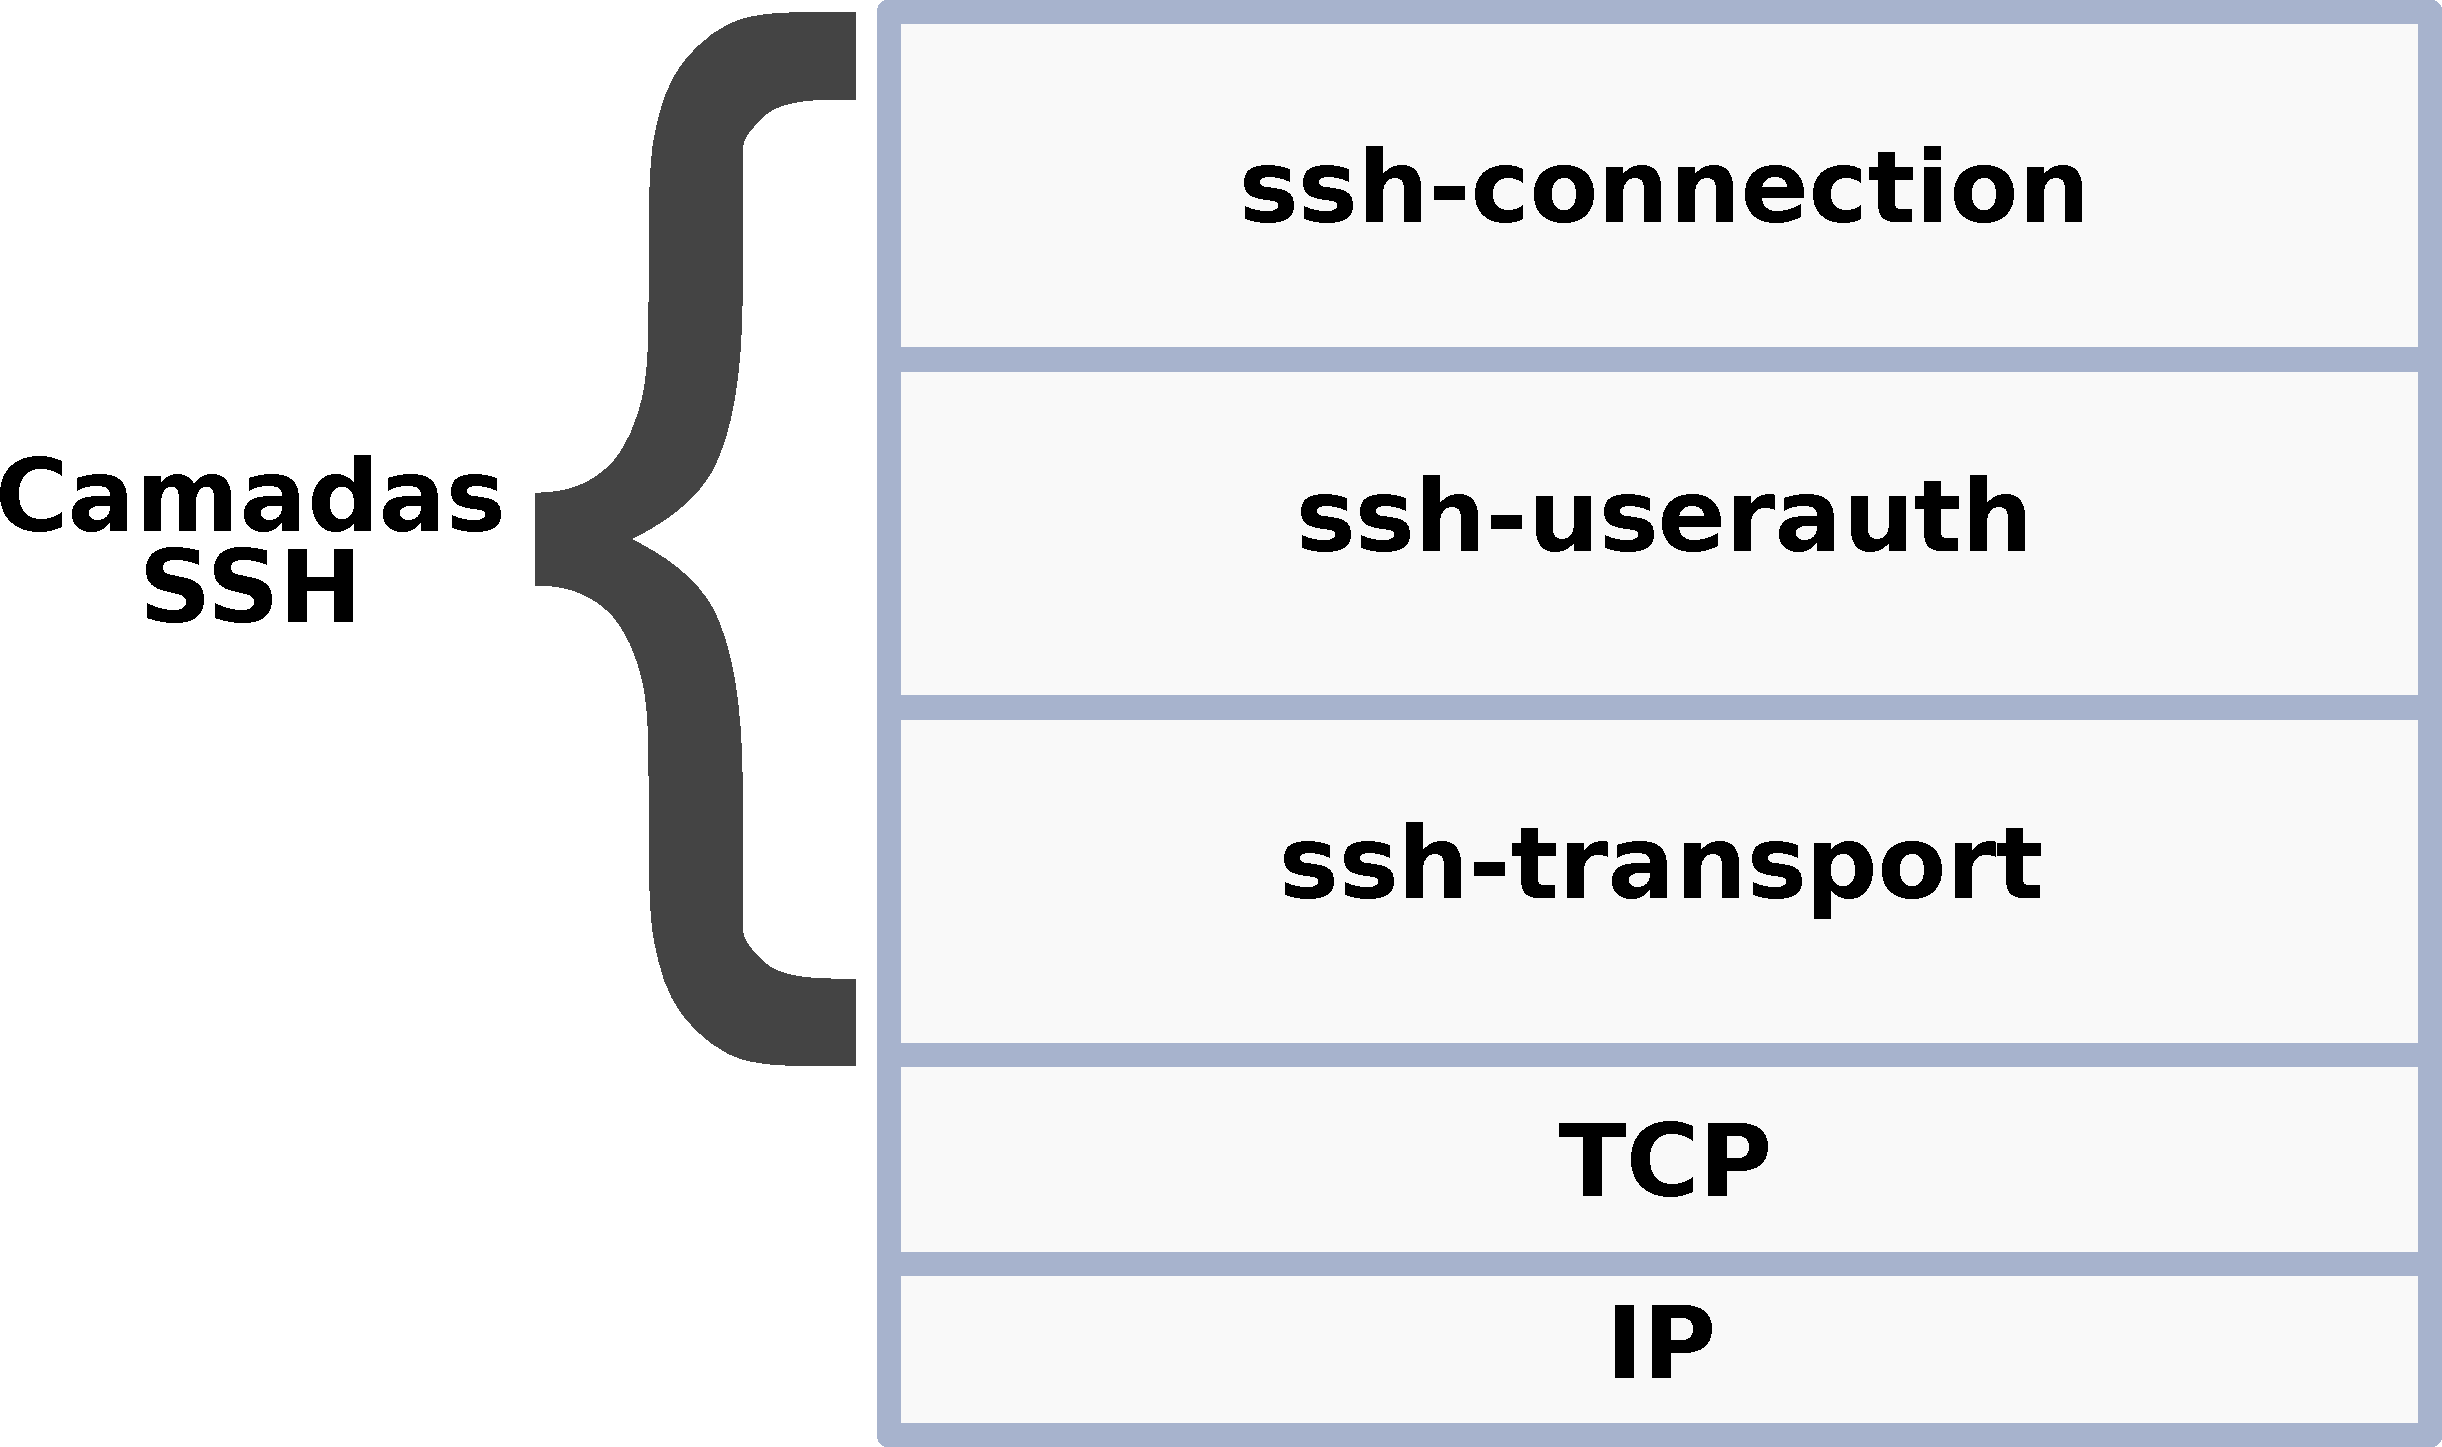
\includegraphics[width=0.3\textwidth]{ssh_layers}
  \caption{Camadas SSH \citep{opensshhood}}
  \label{fig:openssh_layer}
\end{figure}

Dado a enorme importância do OpenSSH, esse é alvo de constantes ataques e
consequentemente recebe diversos aprimoramentos. Como resultado, algumas CVEs
foram criadas e resolvidas no OpenSSH. Dentre as CVEs destacamos: TODO :(

% TODO: Destacar

Do ponto de vista do uso de tal aplicação para validar propostas de abstrações
de processos, destacamos que essa pode ser usada para demonstrar ganhos de
segurança e controle de acesso a memória. Uma abordagem é partir de uma versão
antiga do OpenSSH que não tem a correção para alguma vulnerabilidade e
demonstrar que a nova abstração sugerida consegue resolver o problema. Note que
os pontos mais fracos do OpenSSH podem ser destacados:

\begin{itemize}
  \item Acesso a chave é uma região crítica e deve ter o seu acesso restrito;
  \item Potencial vazamento de dados;
  \item Escalada de privilégios.
\end{itemize}

\section{Outras Aplicações para Avaliar Diferentes Aspectos}

As propostas de novas abstrações de processos podem levar benefícios para
outras áreas além das mostradas nas Seções \ref{sec:web_server} e
\ref{sec:com_enc}. Por esse motivo, apresentamos algumas ferramentas que são de
ampla utilização no mercado e que podem ser utilizadas na validação da
utilidades de algumas das novas abstrações sugeridas.

\subsection{Redis}

Escalar alguns sistemas não é uma tarefa trivial e exige constantes
customizações. Como resultado dessa necessidade, surgiu o sistema Redis que
consiste da ideia de utilizar um sistema que pode ser um cache e ao mesmo tempo
um sistema de armazenamento utilizando a memória principal (RAM) com o objetivo
de levar ganhos de desempenho para a aplicação. O Redis também salva os dados
da memória para o disco, isso permite que posteriormente ele consiga
reconstruir o sistema na memória.

O Redis é famoso por utilizar como forma de armazenamento o esquema de
chave-valor (\textit{key-value}). Essa técnica permite o armazenamento dos dados na
forma de um par que consiste de uma chave identificadora e um valor associado a
chave. Quando um valor-chave é salvo, isso significa que o par está presente na
RAM, no Redis, uma chave tem que ser uma string mas seus valores podem ser de
vários tipos diferentes, dentre as abstrações de dados suportadas destacam-se:

\begin{itemize}
  \item Lista de strings
  \item Conjunto de strings
  \item Conjunto de strings ordenadas
  \item Tabelas de hash na qual a chave e valor são strings
  \item HyperLogLogs
  \item Stream de entradas com grupos de consumidores
  \item Dados Geoespaciais
\end{itemize}

O tipo utilizado no valor determina qual operação é possível de ser aplicada.
De forma geral o Redis permite realizar operações de alto nível (e.g.,
operações do lado do servidor, uniões e diferenças).

A Figura \ref{fig:redis} apresenta uma visão de geral da organização do Redis.
Repare que o Redis fornece uma interface de interação do lado do cliente (via
linha de comando ou API) e possui um servidor que é responsável por lidar com
os dados.  O servidor é responsável por gerir os dados na memória e em disco,
por isso a sua implementação faz constante uso da criação de processos (via
chamada de sistema \texttt{fork()}). Basicamente, toda vez que um armazenamento
é necessário, o Redis faz um \texttt{fork()} do processo pai, em seguida o
processo filho da início ao processo de escrita em disco enquanto o processo
pai continua realizando as suas tarefas. 

\begin{figure}[!h]
  \centering
  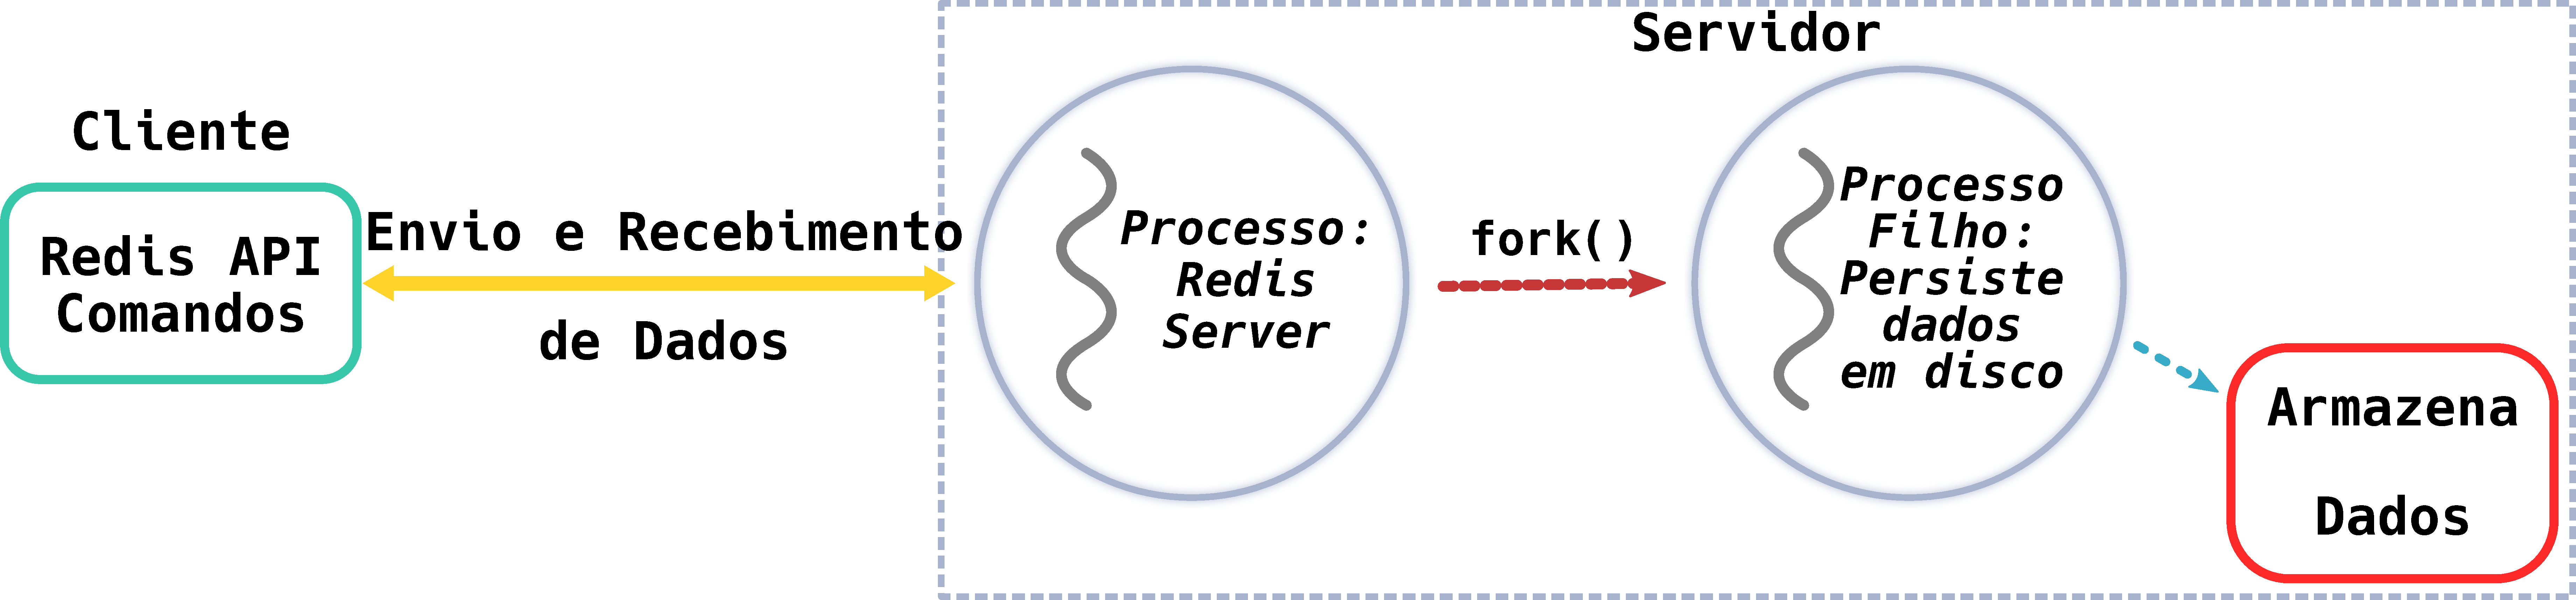
\includegraphics[width=\textwidth]{redis_overview}
  \caption{Visão geral do funcionalmento do Redis}
  \label{fig:redis}
\end{figure}

Um dos aspectos mais interessante do Redis, da perspectiva das novas abstrações
de processo, é a persistência dos dados. O Redis fornece três formas
\citep{redisio}: \textit{Relational Database (RDB)}, \textit{Append-Only-File
(AOF)} e comando SAVE. O RDB faz uma cópia de todos os dados presentes na
memória para o disco, por padrão, o Redis escreve os dados a cada dois
segundos. Repare que o RDB pode causar perda de dados em caso de mal funcionar,
uma alternativa seria configurar o Redis para fazer mais escritas, contudo isso
eleva consideravelmente o consumo de memória pela natureza do uso de
\texttt{fork()}. O AOF registra todas as operações de escritas feitas pelo
servidor, logo tudo é persistido. O AOF tem o problema de que pode ser mais
lento do que o RDB a depender da política de sincronização adotada e também
consumir mais memória.  Por fim o comando SAVE força o servidor a criar um
\textit{dump} dos dados no momento em que foi solicitado.

% TODO: Vale a pena dar um certo nível de detalhes do código? Não é tão complicado fazer isso, mas preciso ter certeza antes se vale a pena
% Além da referencia do "Redis: under the hood" tem esse artigo aqui: http://robertlehmann.de/img/redis.pdf

\subsection{Garbage Collection (GC)}
\label{sec:gc}

Várias linguagens de alto nível possuem mecanismos de gerenciamento recursos
(e.g., memória, processamento paralelo, datas, etc) que garantem a portabilidade
da aplicação e removem a complexidade de ter que gerenciar recursos de baixo
nível. Dentre as vantagens de tais tecnologias, destacam-se o fato de que o
programador pode manter o foco nas características da aplicação e também reduz
a chances de erros graves. O Java é o principal representante desse tipo
linguagem, fornecendo mecanismos de gerenciamento automático da memória e sendo
portável para múltiplas plataformas. Por uma questão de simplicidade, iremos
adotar o Java para as discussões desta seção. Todas as flexibilidades
oferecidas pelo Java deve-se ao uso da \textit{Java Virtual Machine} (JVM) que
fornece elementos para a manipulação dos recursos do SO. Um dos principais
elementos da JVM é o \textit{Garbage Collection} (GC), cujo a principal tarefa
consiste em abstrair o gerenciamento de memória da aplicação de forma que ela
não tenha que lidar com tal aspecto (alocar e desalocar). Dado o seu impacto, o
GC tem sido alvo de constantes otimizações ao longo dos anos e esse é um
elemento que pode se beneficiar de novos recursos oferecidos por extensões
abstrações de processos.

O GC é uma aplicação que é parte da JVM executando junto com a aplicação.
Independentemente do algoritmo de gerenciamento de memória implementado pelo
GC, todos eles definem o termo \boldAndIndex{Stop the World (STW)} ou
\textit{Parar tudo} \citep{gc_pauseless}. O STW é uma operação realizada pela
JVM  na qual todas as threads da aplicação são suspensas para que o GC execute,
em outras palavras, a única thread executando será a do coletor. Note que o GC
requer pausa para funcionar, isso é preciso pois seus algoritmos precisam que
aplicação não faça nenhuma atualização da memória durante uma das fases do
processo de limpeza da memória.

Existem diversos algoritmos que podem ser adotados pelo GC, contudo podemos
generalizar três etapas gerais: \textit{Marking}, \textit{Sweep} e
\textit{Compact}. A etapa de \textit{Marking}, também conhecida por pintura,
consiste em inspecionar os objetivos na memória para verificar quais ainda são
considerados vivos. Para determinar se um objeto está vivo o GC começa por
lementos conhecidos como objetos raiz ou \textit{Garbage Collection Roots}, os
seguintes componentes são considerados como um GC root: variáveis locais,
entrada de parâmetros, threads ativas, campos estáticos e referências JNI
\citep{gc_basics}. Partindo de um GC root, o GC atravessa o grafo dos objetos
alcançáveis e para cada elemento que consegue acessar ele “pinta” a referência
como viva. A Figura \ref{fig:gc_alg} ilustra o algoritmo descrito. No contexto
do GC, o processo de parar as threads para que a JVM possa executar a etapa de
\textit{Marking} recebe o nome de \textit{safe point} (ponto seguro) e essa
gera um STW. O tamanho da pausa é definido pela quantidade de objetos
alcançável e o seu tamanho no \textit{heap}.

\begin{figure}[!h]
  \centering
  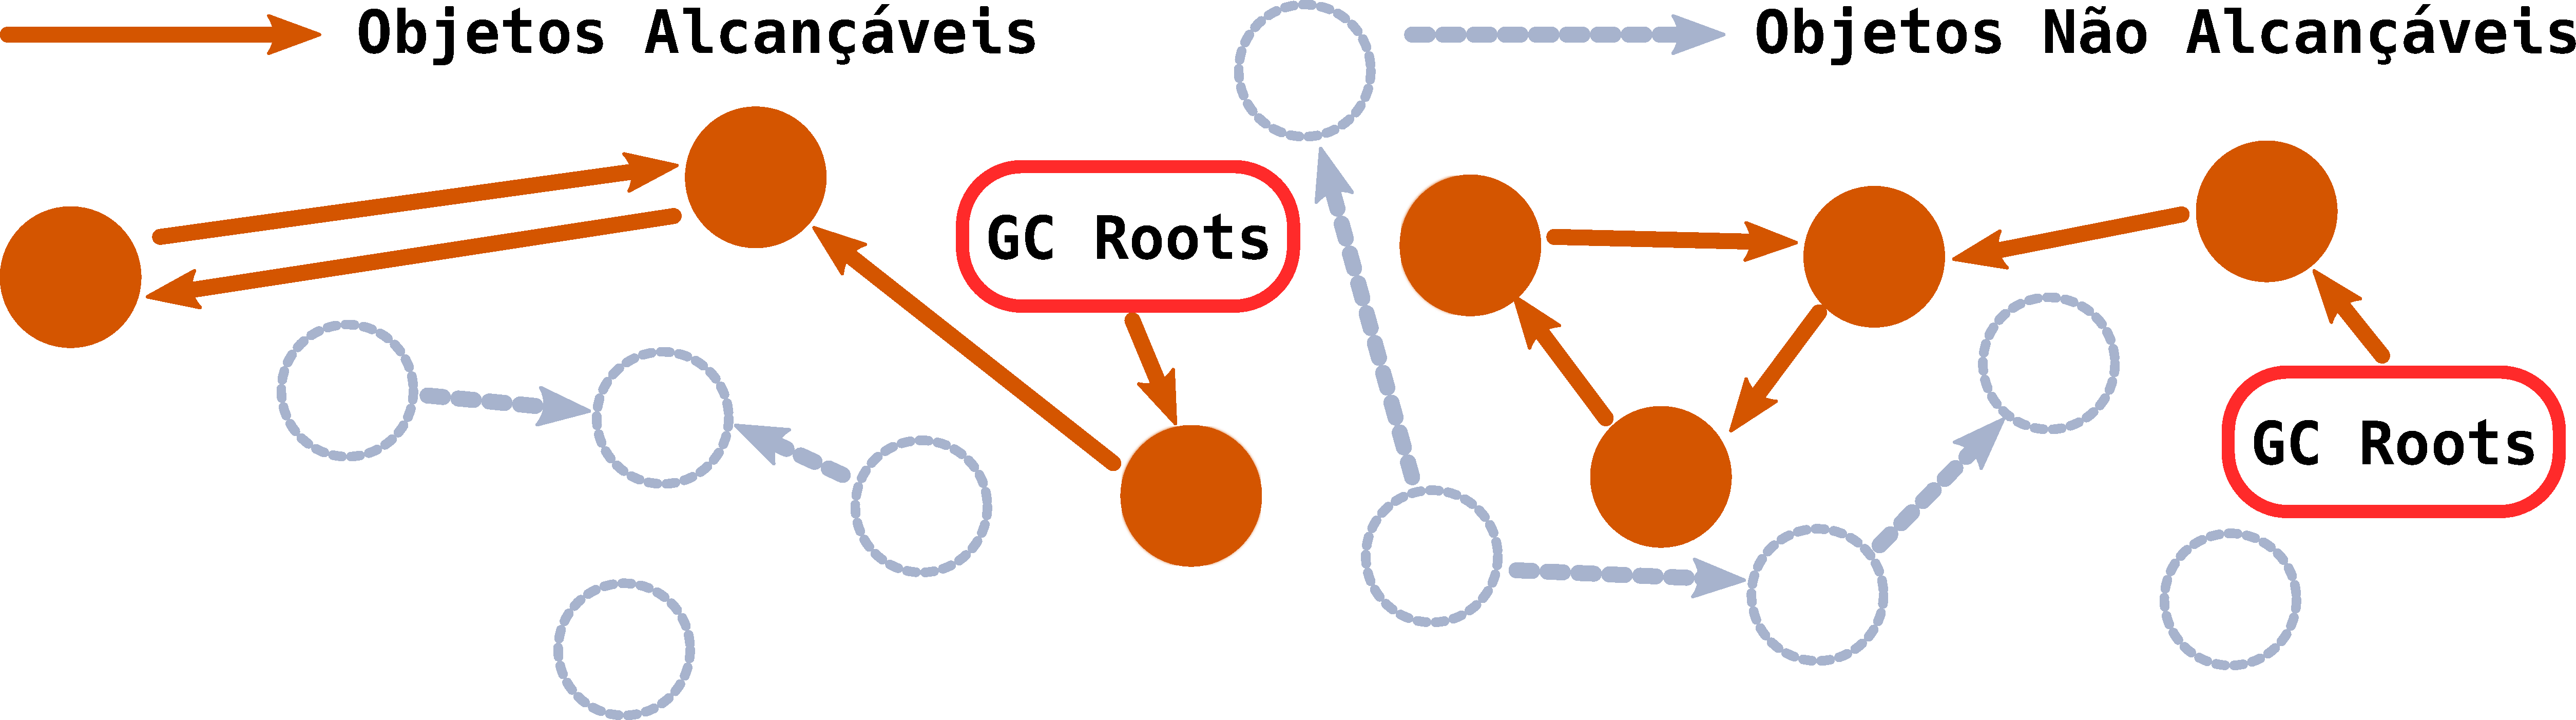
\includegraphics[width=\textwidth]{gc_algoritmo}
  \caption{Algoritmo de pintura da memória\citep{gc_basics}}
  \label{fig:gc_alg}
\end{figure}

Depois da etapa de pintar os objetos na memória, entra em ação a etapa de
remover os objetos que não foram pintados; note que essa etapa pode acontecer
em paralelo ou não, depende do algoritmo adotado. O processo de remoção pode
gerar fragmentação na memória, o que pode representar um problema uma vez que o
GC pode não encontrar espaços de memória grande o suficiente para outros
objetos. Por isso também existe uma fase de compactação na qual o GC realoca os
objetos pintados para liberar espaço contíguo. Contudo, para que a compactação
aconteça corretamente as referências dos objetos tem que ser atualizadas uma
vez que a posição física dos objetos mudou. O processo de atualizar as
referência chama-se remapeamento e ele precisa examinar toda a memória para
realizar os ajustes, note que a etapa de compactação eleva o tempo de STW. A
Figura \ref{fig:gc_mem} apresenta uma visão da memória durante as três etapas
descritas.

\begin{figure}[!h]
  \centering
  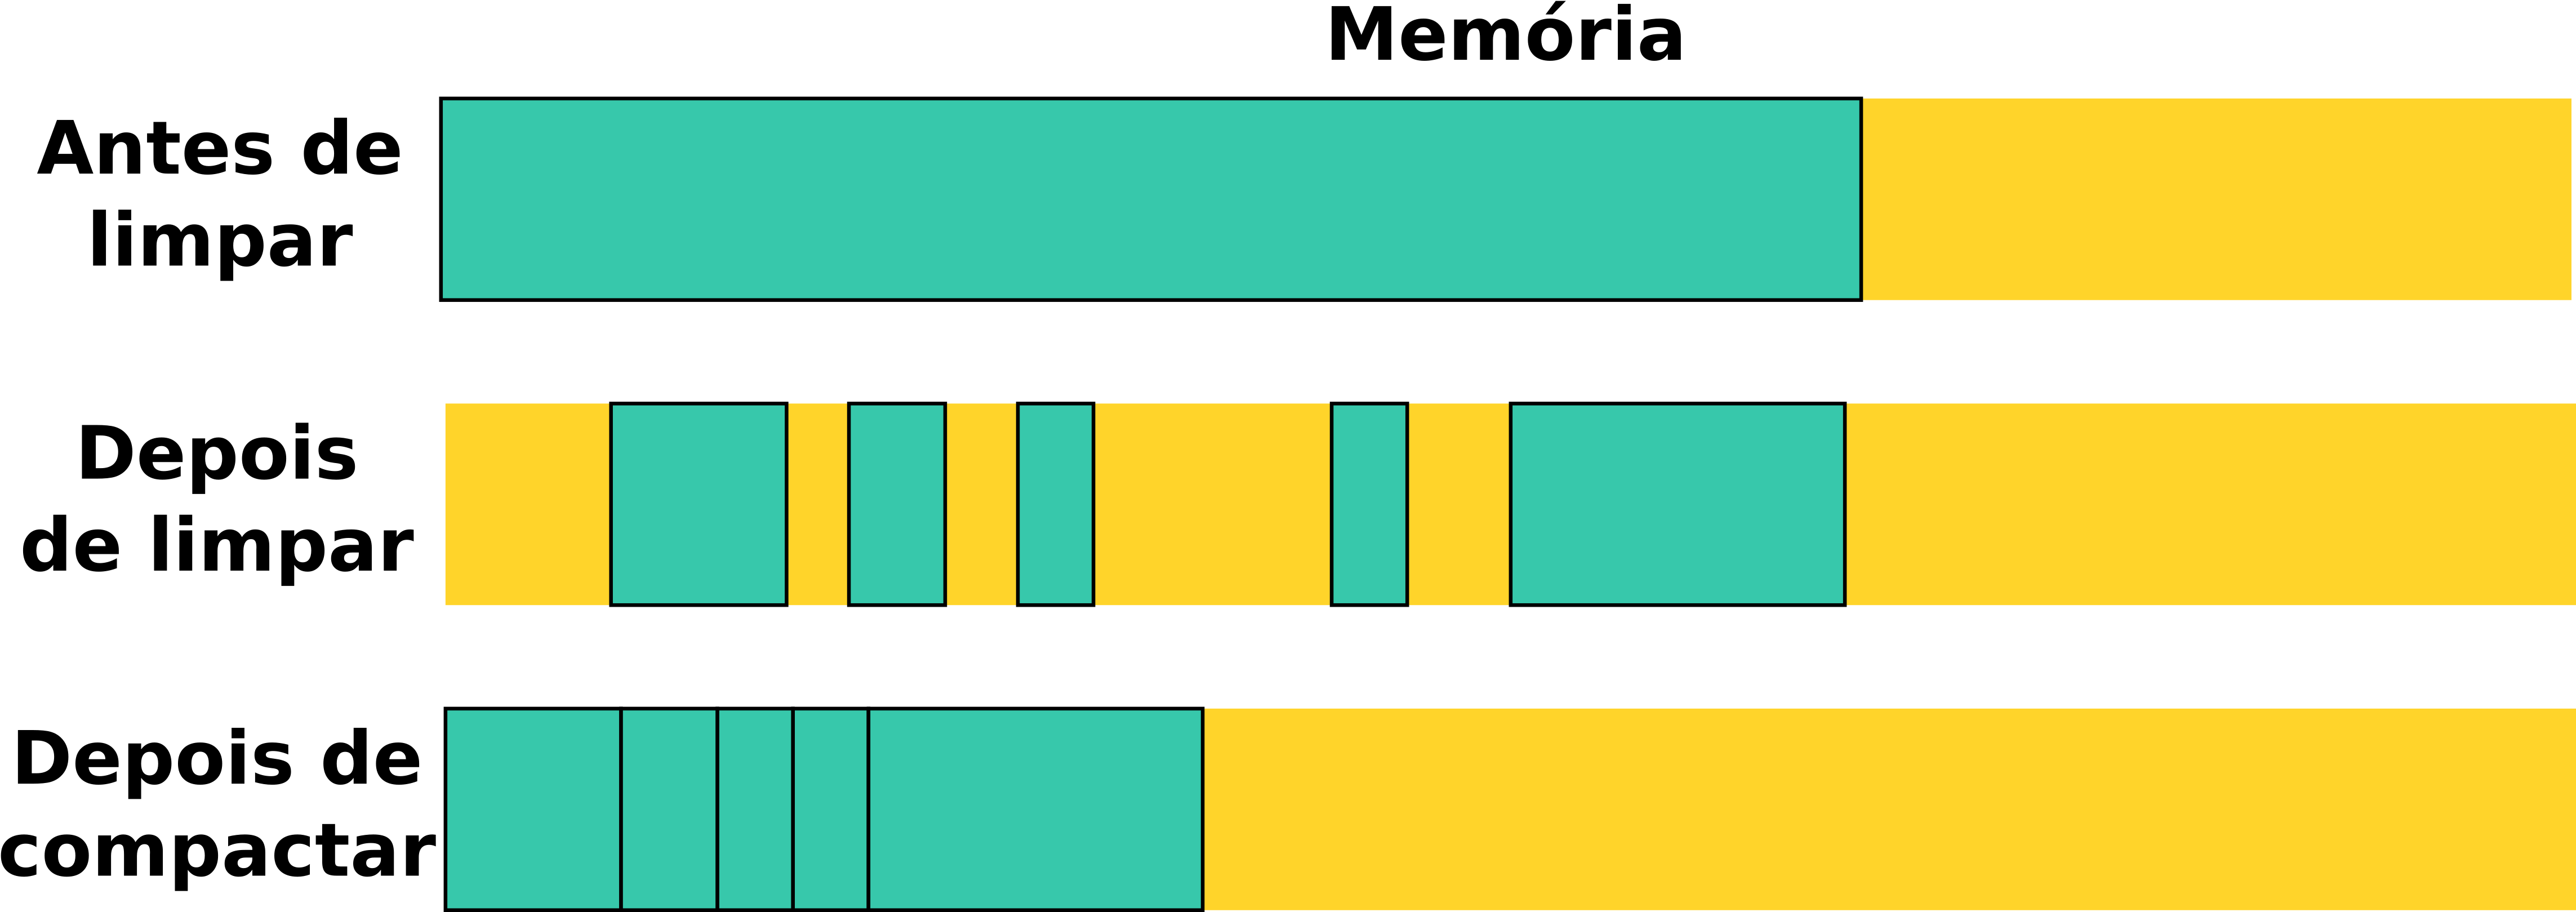
\includegraphics[width=0.8\textwidth]{gc_memory}
  \caption{Visão da memória durante a aplicação do algoritmo de GC\citep{gc_basics}}
  \label{fig:gc_mem}
\end{figure}

Vale salientar que existem diversos algoritmos de GC, cada um com suas
vantagens e desvantagens; nosso objetivo nessa seção é apenas ilustrar o
potencial de uso de tal aplicação para validar novas abstrações de processos.

\section{Discussão Sobre as Aplicações}
\label{sec:disc_app}

Desde o começo deste capítulo até está seção apresentamos algumas aplicações
destacando o seu funcionamento, estruturas básicas e os recursos exigidos por
elas. Contudo, o nosso principal objetivo é verificar quais tipos de benefícios
e validações que tais aplicações podem fornecer para o avanço das pesquisas em
novas abstrações de processos. Cada tipo de aplicação pode ser útil para
demonstrar algum aspecto da nova abstração, mas idealmente é interessante
evidenciar que as demais aplicações apresentadas também não sofrem com a nova
abstração.

O Apache e o Nginx são aplicações cujo o objetivo é servir requisições feitas
pelos usuários, ou seja, são servidores web. Esse tipo de aplicação normalmente
oferece opções para que sejam amplamente configuradas de forma a atender os
requisitos do usuário da melhor maneira possível. Tais aplicações são
especializadas para tirar o máximo de proveito possível dos recursos de hardware,
uma vez que servidores web podem lidar com enormes cargas de requisições
levando a um ostensivo uso do hardware. Nesse tipo de aplicação é comum que
ocorra um amplo consumo da memória e que a CPU esteja próxima do 100\% de
utilização em situações estresse (muitos usuários acessando).  Note que quanto
mais tempo uma requisição vive, mais memória é consumida, por isso é desejável
que as requisições sejam atendidas o mais rapidamente possível. Por sua vez o
SO tem que manipular diversos aspectos relacionados a memória, processos e
arquivos. Por esse motivo, utilizar esse tipo de software como prova de
conceito para demonstrar a eficácia de uma nova abstração de processos é algo
extremamente desejável. Essas aplicações podem ser utilizadas para mostrar que
o comportamento da alteração na abstração de processos em uma situação de alta
demanda. Contudo é importante ressaltar que os testes realizados em tais
ferramentas devem gerar uma carga substancial para que a configuração padrão
tenha que ser alterada. Esse aspecto é fundamental uma vez que não existe
grande valor em demonstrar algo usando tais ferramentas com uma carga pequena,
pois isso pouca ajuda na verificação dos reais impactos gerados pela nova
extensão do processo.

O Apache também possuí um ambiente que permite testar processos e threads de
forma equivalente. Tal característica é interessante para comparar novas
abstrações diante de dois modos de execução amplamente utilizados. De forma
similar o Nginx usa outro modelo chamado de \textit{event} que também
representa outra contexto para validação. Da forma como o Apache e o Nginx
manipulam requisições, podemos dizer que o primeiro fornece um isolamento
horizontal enquanto o segundo proporciona isolamento vertical. O isolamento
horizontal vem do fato de que um processo cria vários outros e o vertical vem
da criação de um único processo por núcleo do processador durante a
inicialização. Esses dois níveis de isolamento podem ser úteis para demonstrar
que uma nova abstração pode melhorar o isolamento sem degradar o desempenho.

O Apache trabalha com diversos \textit{plugins} que são acoplados ao código
principal dinamicamente. Essa junção tem uma boa relação desempenho e
flexibilidade, mas também elevam as chances de quebrar o Apache.  Portanto o
sistema de \textit{plugins} do Apache fornece um bom elemento de validação para
aquelas abstrações que visam trazer isolamento e recuperação.

Várias propostas de extensão da abstração de processos sugerem algum ganho de
segurança por meio do controle fino ou isolamento de pedaços da memória. Nesse
sentido o OpenSSH e OpenSSL são ferramentas interessantes, já que possuí os
requisitos de segurança adequado para a validação das novas abstrações. Em
especial, ambas as aplicações tem diversas CVEs associadas a si com correções
disponíveis a partir de uma versão especifica. Portanto uma proposta de
melhoria na abração de processo que eleva a segurança pode demonstrar o seu
real valor em uma dessas aplicações.

O Redis por sua vez é uma aplicação que trabalha com grandes quantidade de
dados na memória e que tem um excelente desempenho em situações de forte
demanda. Essas características fazem do Redis uma excelente ferramenta para
demonstrar novas técnicas de compartilhamento da memória. Além disso, um dos
objetivos do Redis é auxiliar na escalabilidade das aplicações por isso é
desejável que o mesmo reaja rapidamente a qualquer problema. Nesse contexto,
abstrações de processos novas que tragam melhorias no tempo recuperação de uma
aplicação em caso de falha podem usar o Redis com instrumento de validações.

Novas abstrações de processos podem entregar ganhos de desempenho para as
aplicações por utilizar algum recurso de hardware ou mesmo fornecer uma nova
estrutura de dados para a aplicação. Tal otimização pode ser demonstrada em um
GC uma vez que esse tipo de aplicação faz uso de vários algoritmos que dependem
de certos dados fornecidos pelo SO. Como exemplo disto, a fase de compactação
pode ser otimizada se o endereço virtual for mantido e apenas o endereço físico
alterado \citep{pauseless}.

A Tabela \ref{tab:app_alvos} busca resumir quais aplicações podem ser usadas
para demonstrar algum aspecto da nova abstração de processos. Além disso essa
seção inteira responde a pergunta RQ3 uma vez que apresenta e discute diversas
aplicações. Por fim repare da Tabela \ref{tab:app_alvos} que o Apache é uma das
ferramentas que melhor pode ser usada para demonstrar os aspectos de uma nova
abstração de processos. No Capítulo \ref{cap:estudo-de-caso} aprofundamos a
validação utilizando o Apache para testar o MVAS. 

\begin{table}[]
\small
\centering
  \begin{tabular}{|@{}c@{}|@{}c@{}|@{}c@{}|@{}c@{}|@{}c@{}|@{}c@{}|@{}c@{}|}
  % TOPO DA TABELA
  % |M{2.5cm}|M{2.5cm}|M{2.5cm}|
  \hline
  \multicolumn{1}{|l|}{\diagbox[width=2.5cm, height=2cm]{App}{Alvo}} &
    % Troca de contexto
    \multicolumn{1}{@{}c@{}|}{\begin{tabular}[c]{@{}c@{}}Controle\\fino da\\Memória\end{tabular}} &
    % Persistência de processos
    \multicolumn{1}{@{}c@{}|}{\begin{tabular}[c]{@{}c@{}}Consumo\\ de CPU \end{tabular}} &
    % Controle fino de privilégios
    \multicolumn{1}{@{}c|}{\begin{tabular}[c]{@{}c@{}}Consumo \\de Memória \end{tabular}} &
    % Segurança
    \multicolumn{1}{@{}c|}{Segurança} &
    % Recuperação
    \multicolumn{1}{@{}c|}{Recuperação} &
    % Otimização
    \multicolumn{1}{@{}c|}{Otimização} \\ \hline \hline
  % Início da tabela
  Apache  &                             & \ding{52}\ding{52}\ding{52} & \ding{52}\ding{52}\ding{52} & \ding{52}\ding{52}            & \ding{52}\ding{52} & \ding{52}\ding{52}          \\ \hline
  Nginx   & \ding{52}                   & \ding{52}\ding{52}          & \ding{52}\ding{52}          & \ding{52}                     & \ding{52}          & \ding{52}\ding{52}          \\ \hline
  OpenSSL & \ding{52}\ding{52}\ding{52} &                             &                             & \ding{52}\ding{52}\ding{52}   &                    &                             \\ \hline
  OpenSSH & \ding{52}\ding{52}\ding{52} &                             &                             & \ding{52}\ding{52}\ding{52}   &                    &                             \\ \hline
  Redis   &  \ding{52}\ding{52}         &                             & \ding{52}\ding{52}          &                               & \ding{52}          & \ding{52}                   \\ \hline
  GC      &                             & \ding{52}                   & \ding{52}\ding{52}          &                               &                    & \ding{52}\ding{52}\ding{52} \\ \hline
  \end{tabular}
\caption{Relação aplicações e alvos}
\label{tab:app_alvos}
\end{table}


\section{Microbenchmark}
\label{sec:micro}

\textit{Microbenchmarks} tem por objetivo mensurar e fornecer meio para
analisar uma única característica do objeto de estudo. Essa forma de validação
traz inúmeras vantagens, dentre elas: facilita o processo de desenvolvimento,
mostra o impacto em um único elemento de forma a facilitar a análise e são
relativamente simples de serem implementados. Contudo, a principal desvantagem
encontra-se no fato de que eles não ajudam a revelar o impacto geral do objeto
alvo. Por esse motivo é interessante trabalhar com um conjunto de
\textit{microbenchmark} e também com validações usando aplicações (como
descrito na Seção \ref{sec:disc_app}). Expandindo o contexto dos
\textit{microbenchmarks} para o subconjunto da pesquisa sobre abstrações de
processos, queremos destacar aquelas validações que lidam com a memória,
sobrecargas extra e impactos na utilização de certos recursos de hardware.

No Capítulo \ref{cap:trabalhos-analisados} apresentamos diversas propostas que
buscam de alguma maneira lidar com os mecanismos de acesso a memória. Várias
dessas propostas permitem o controle fino da memória ou algum ganho de
segurança na qual os autores normalmente demonstram por meio da alteração de
algumas aplicações (e.g., OpenSSL ou OpenSSH). Contudo, alterações no
gerenciamento da memória podem incorrer em erros e em problemas de desempenho.
Nesse sentido alguns \textit{microbenchmarks} podem ser extremamente oportuno
para validar o uso de novas abstrações de processos que lidam com a memória.
Com base em todos os trabalhos analisados no Capítulo
\ref{cap:trabalhos-analisados}, extraímos os seguintes itens:

\begin{description}

  \item[Medir tempo gasto com novos mecanismos de alocação de memória:]

Algumas propostas criam mecanismos de alocação de memória contendo
características novas, por isso é interessante comparar os mecanismos
propostos pelo pesquisador utilizando como base a forma padrão de alocação
(e.g., \texttt{malloc()} e \texttt{calloc()}). Tendo os valores base extraído
das operações já consolidadas e os valores coletados do modelo proposto,
torna-se possível ter um critério para compreender o real impacto da mudança.
Vale observar que esse tipo de \textit{microbenchmark} precisa ser feito com
múltiplas cargas de tamanhos variados, no minimo, espera-se cargas na ordem dos
KBs, MBs e GBs.

  \item[Medir tempo gasto com operações de litura e escrita:]

Mensurar o tempo de leitura e escrita em uma memória usando os mecanismos
padrão é importante para ter o custo de acesso base. Tal informação deve ser
utilizada para comparar com novas propostas de abstrações de processos que
adicionam camadas extras para acessar a memória (e.g., Nooks e Wedge).
Novamente é importante que várias cargas de trabalho sejam utilizadas.

\end{description}

Algumas propostas sugerem a adição de novas chamadas de sistema que adicionam
novos modelos de programação (e.g., lwC e MVAS). Apesar das chamadas de sistema
serem relativamente rápidas, essas adicionam \textit{overhead}. Por isso é
desejável que o pesquisador identifique alguma \textit{syscall} padrão que tem
algum nível de similaridade com a nova chamada que ele está propondo; assim ele
pode realizar medições do tempo total gasto da chamada padrão para ter um valor
base para comparar com a nova chamada. Contudo, existem casos em que a nova
chamada representa algo totalmente novo e que não faz sentido comparar com
qualquer outra chamada já existente. Independentemente de existir ou não uma
chamada base é desejável que o pesquisador execute \textit{microbenchmarks} que
validem:

\begin{description}
  \item [Aferir tempo total gasto na chamada:]

Espera-se que o tempo total da chamada seja medido considerando-se o cenário em
que a chamada é feita dezenas, centenas e milhares de vezes. Esse tipo de
parametrização é importante na validação do comportamento da chamada sob
diferentes cargas.

  \item [Aferir tempo total gasto da chamada em um contexto de concorrência:]

Testes realizados no contexto de concorrência auxiliam na validação de como
novas chamadas se comportam. Novamente, espera-se que tal teste execute
a nova chamada diversas vezes.

  \item [Quantidade de troca de contexto:]

As novas instruções podem fazer com que o número de troca de contexto aumente,
por isso é valioso medir tal aspecto referente a nova chamada.

\end{description}

Várias propostas propõem um novo hardware (e.g., Mondrix) ou uma mudança na
forma como um dispositivo é usado, o que torna importante validar alguns
aspectos de uso. Contudo, para a questão do \textit{microbenchmark} vamos
considerar apenas os aspectos referentes a reutilização do hardware de
virtualização uma vez que consideramos que tal técnica tem amplas chances de
ser adotada (discutimos esse aspecto com mais detalhes no Capítulo
\ref{cap:analise-sobre-abstracoes-de-processos}). Nesse contexto, dois
elementos devem ser medidos:

\begin{description}

  \item [Custos de operações que executam \textit{VM Entry} e \textit{Exit}:]

Chamadas que utilizam recursos de virtualização tem o custos para entrar e sair
do kernel. Mensurar tal custo é útil para analisar quais contextos valem a pena
ou não utilizar os recursos de virtualização.

  \item [Medir o uso de EPT:]

Quando se utiliza a EPT, espera-se que o total de \textit{TLB misses} se eleve
uma vez que em muitos casos é preciso procurar por dois níveis de chamadas
~\citep{belay}. Portanto, torna-se interessante medir o tempo total gasto
quando a EPT é usada sob diferentes cargas.

\end{description}

Por fim é importante ressaltar que vários dos \textit{microbenchmark} devem
utilizar recursos estatísticos para derivar seus resultados. Por exemplo,
espera-se que cada experimento execute múltiplas vezes e a sua média ou mediana
seja calculada. Além disto a combinação de múltiplos \textit{microbenchmarks}
pode auxiliar consideravelmente na validação de uma nova proposta de abstração.

\section{Discussão}

Recapitulando o objetivo deste Capítulo por meio das perguntas de pesquisa:

\begin{quote}
 \item \textit{RQ3:.} "Quais aplicações podem ser utilizadas para avaliar as nova abstração adicionadas ao SO?"
 \item \textit{RQ4:.} "Qual conjunto de \emph{microbenchmark} pode ser utilizado para auxiliar a entender os impactos de uma nova característica adicionada para as abstrações de processos?"
\end{quote}

Para responder a primeira pergunta, fizemos uma jornada da Seção
\ref{sec:web_server} até a \ref{sec:disc_app} analisando diversas aplicações
amplamente consolidadas. Em especial, a Seção \ref{sec:disc_app} apresentou uma
discussão sobre as vantagens em se utilizar as aplicações para validar as novas
abstrações de processos. A Tabela \ref{tab:app_alvos} buscou relacionar as
aplicações e a área na qual ela auxilia a validar.

Para responder a segunda pergunta, revisitamos todos os trabalhos e buscamos
compilar um conjunto de \textit{microbenchmarks} que auxiliam no processo de
validação.  A combinação de múltiplos \textit{microbenchmarks} auxiliam
mostrando o impacto da alteração de forma mais abrangente, contudo, esse tipo
de validação sozinho não é capaz de revelar os impactos gerais de uma nova
abstração.

Em um cenário ideal, a combinação das validações utilizando as aplicações
discutidas em conjunto com os \textit{microbenchmarks} representam uma boa
cobertura sobre os impactos de uma nova abstração. Por fim, é importante
relembrar que tais validações devem buscar utilizar cargas de trabalho
relevantes para tornar claro os impactos da nova abstração.

\par

\imgchapter[left]{8cm}{chapter_5_title}{Estudo de Caso}
\label{cap:estudo-de-caso}

Neste estudo de caso, nós buscamos atingir três objetivos: (1) garantir a
reprodutibilidade dos resultados, (2) construir uma estrutura que possa ser
estendida para outros cenários e (3) validar os problemas associados a novas
abstrações de processos. Utilizamos uma estrutura para preparar o ambiente
(\emph{deploy}) que é responsável por configurar todas as máquinas alvos
envolvidas nos experimentos. Para automatizar tal passo, decidimos utilizar a
ferramenta \emph{Ansible}\footnote{\url{https://www.ansible.com/}} para
controlar a implantação dos experimentos uma vez que esta é amplamente
utilizada e é relativamente simples de se utilizar. Adicionalmente, temos um
grupo de \emph{scripts} projetados para estressar diferentes
cenários\footnote{\url{https://github.com/LSS-USP/web_server_benchmark}}, esses
\emph{scripts} são baseados em uma ferramenta chamada \emph{Apache Benchmark
Tool} (ab) que por sua vez tem configurações específicas para testar diferentes
aspectos do SO e de um servidor HTTP. Temos uma coleção de programas para
processar todos os dados gerados durante a execução do experimento e produzir
os gráficos. Neste capítulo, apresentamos alguns experimentos e buscamos
validar os benefícios da abordagem utilizando Múltiplos Endereços Virtuais
(MVAS); ou seja, esse capítulo tem como objetivo testar parte do que foi
apresentado no Capítulo~\ref{cap:validacoes}.

\section{Metodologia} \label{sec:metodologia}

\begin{figure}[!h] \centering
  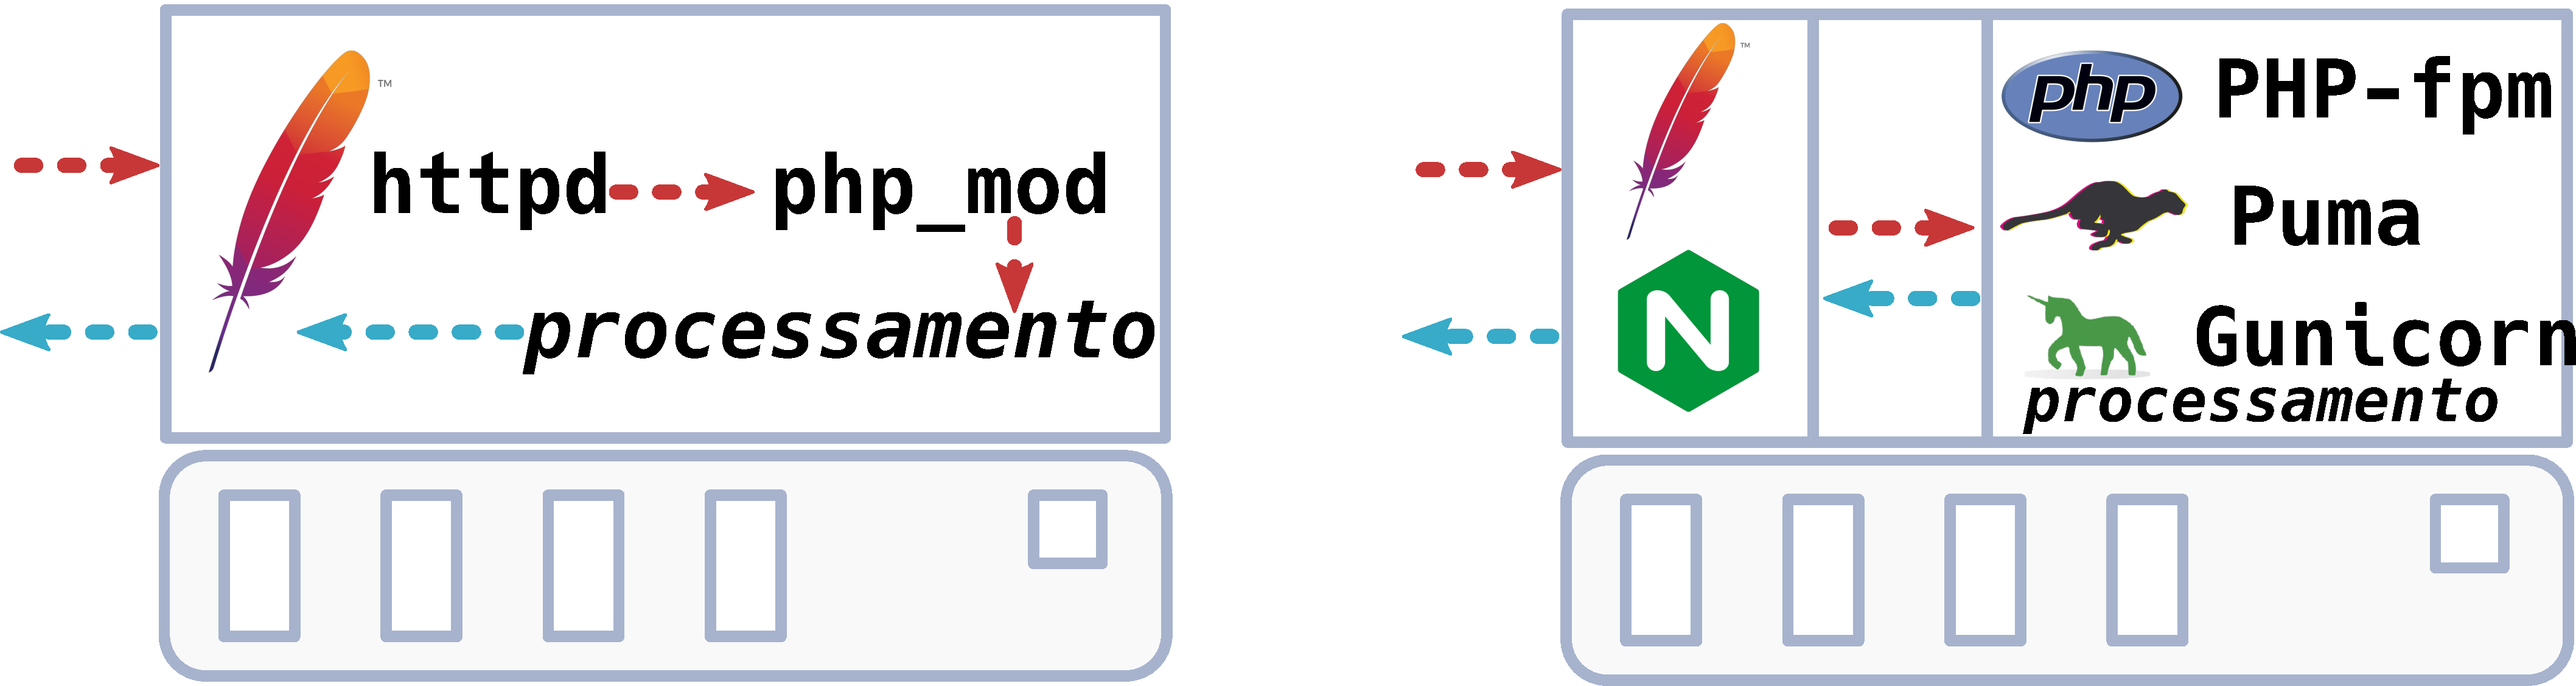
\includegraphics[width=.60\textwidth]{web_server_organization_strategy}
  \caption{Visão geral da organização de aplicações utilizando servidores Web}
\label{fig:web_server} \end{figure}

Atualmente podemos encontrar um grande número de arquiteturas que pode ser
utilizada por um sistema web. A Figura \ref{fig:web_server} ilustra duas
arquiteturas diferentes. A primeira mostra uma situação na qual uma página web
é totalmente manipulada pelo \emph{Apache HTTP Server} (httpd). Basicamente, o httpd manipula uma
solicitação e a passa para um módulo específico responsável por executar um
software (p.ex.: uma página web em PHP é executado por um módulo PHP chamado
\emph{php\_mod}). A segunda arquitetura é um exemplo de página web escrita em
\emph{Ruby on Rails} que é composta por duas camadas: (1) um servidor web para
manipular as requisições que chegaram dos clientes (pode ser o Apache ou
Nginx), (2) um servidor de aplicação responsável por executar um programa (no
exemplo da figura, temos o PUMA que é especializado em executar código Ruby).
Esses exemplos, ilustram que podemos ter diferentes formas de organizar as
aplicações.

\begin{figure}[!h] \centering
  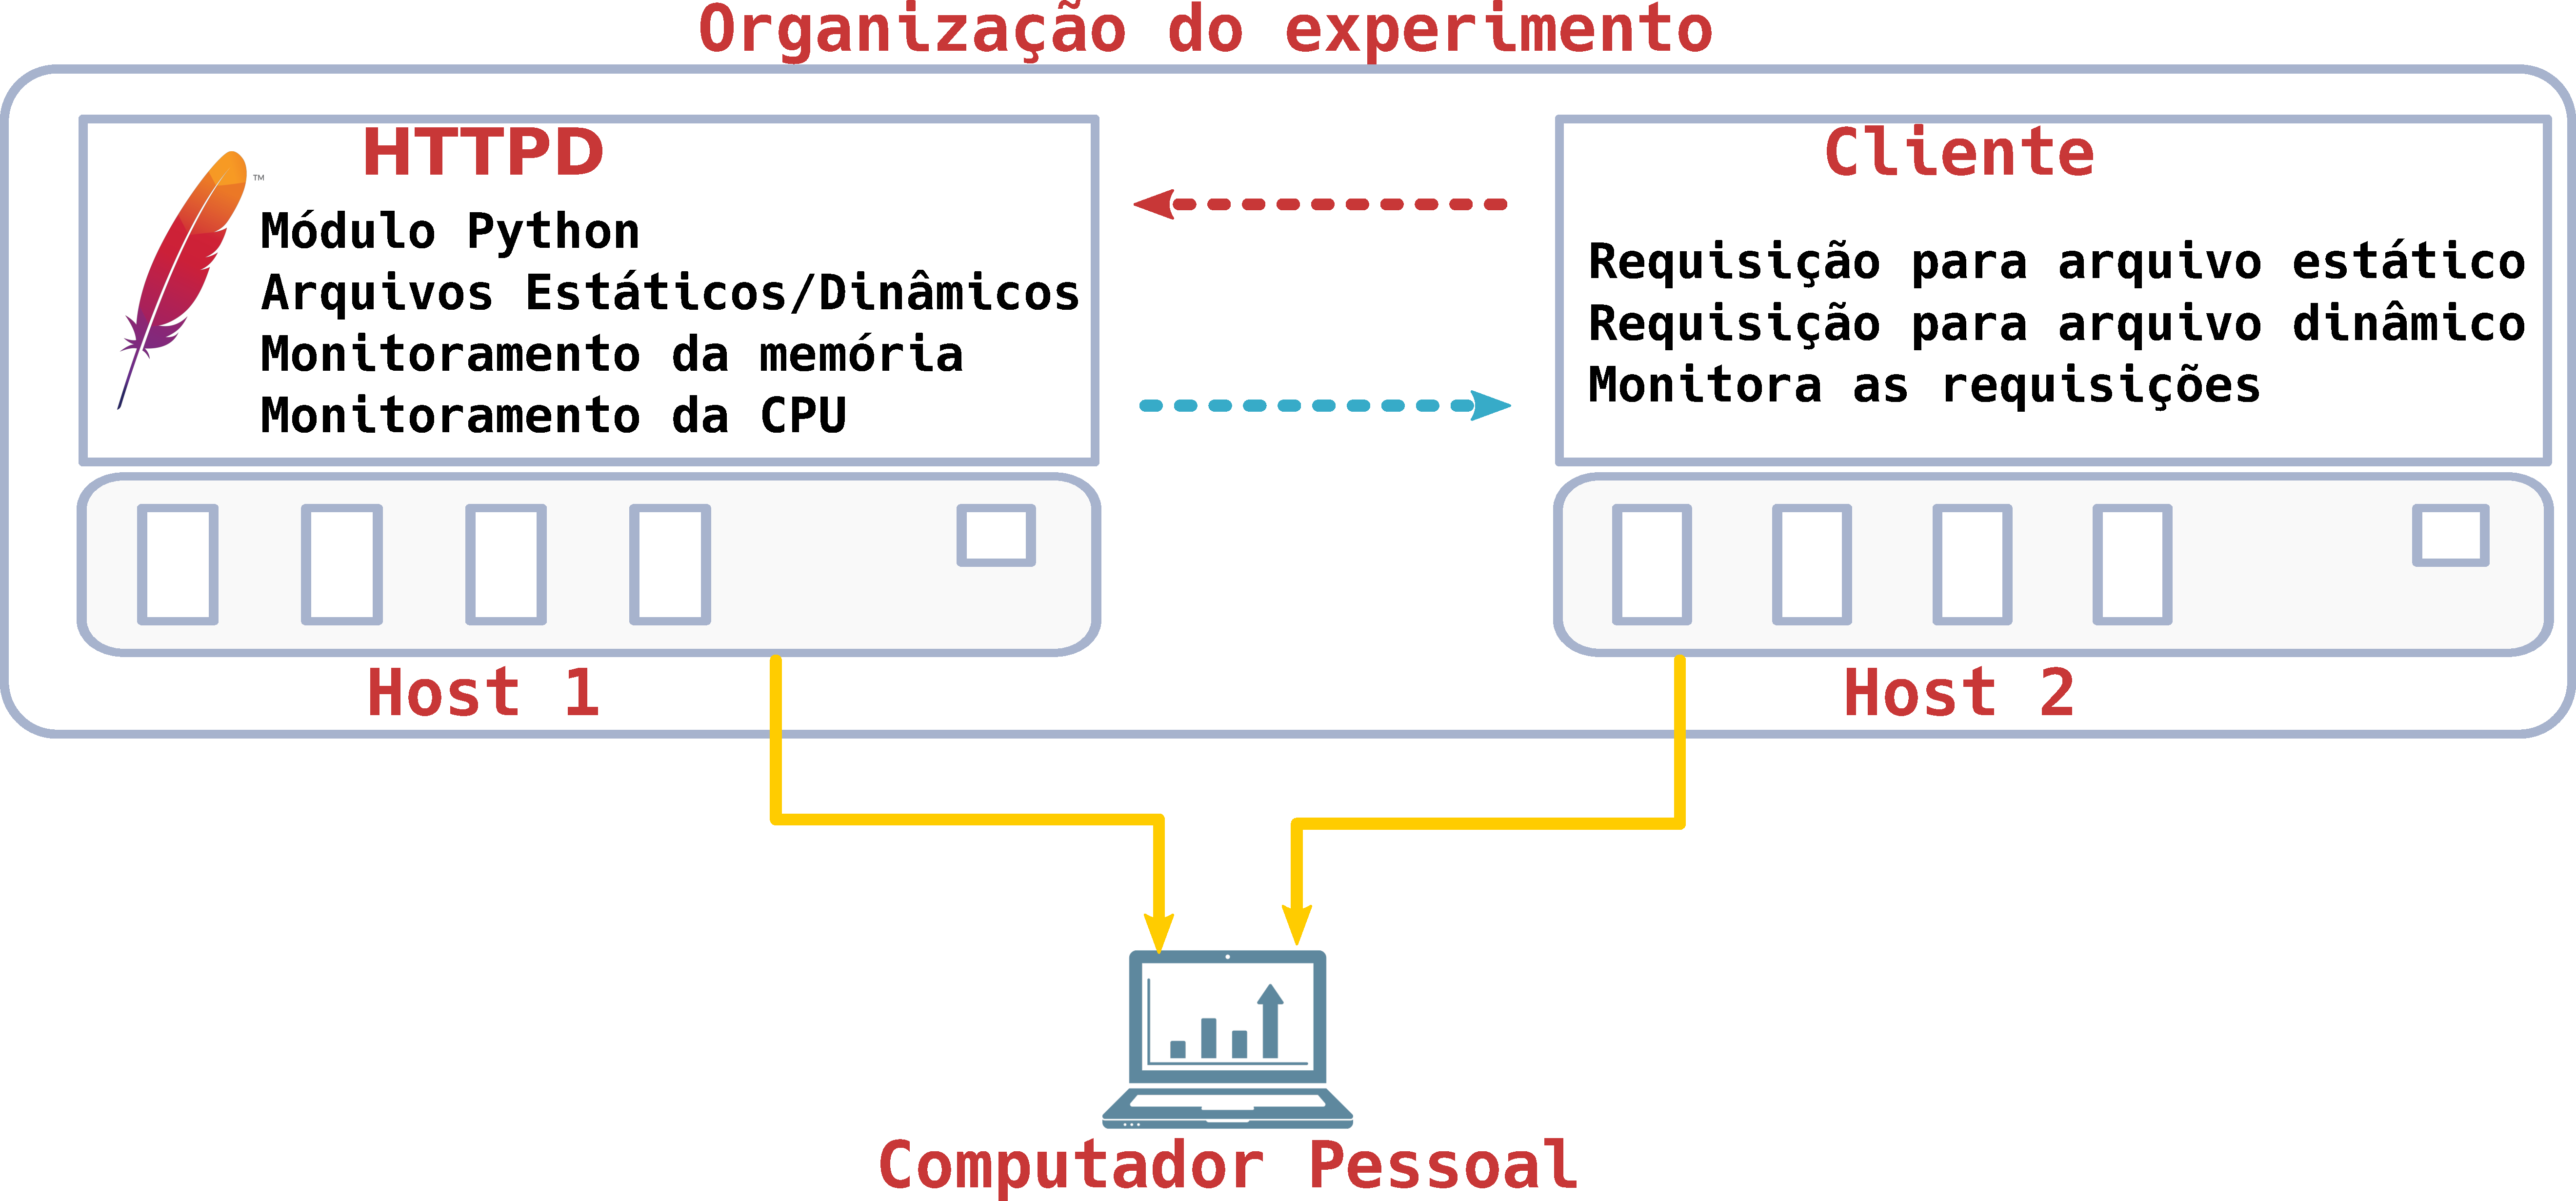
\includegraphics[width=.90\textwidth]{experiment_arhitecture}
  \caption{Arquitetura do experimento} \label{fig:experiment_architecture}
\end{figure}

A Figura  \ref{fig:experiment_architecture}, ilustra de forma geral a estrutura
utilizada para conduzir os experimentos com MVAS. Note que a figura indica duas
máquinas virtuais (Host 1 e Host 2), uma com um servidor web configurado para
dar suporte para uma grande carga de requisições geradas por uma segunda
máquina, que por sua vez, é responsável por simular um grande número de
clientes concorrentes. Ambas as máquinas são conectadas via conexão Gigabit
Ethernet, uma vez que queremos simular múltiplos cliente fazendo requisições
sem ter que se preocupar com questões de sobrecarga da rede.

Nos experimentos, queremos simular uma situação na qual o httpd terá que
lidar com uma grande carga que gere pressão na aplicação e assim eleve a
utilização de recursos de hardware. Com essa ideia em mente, conduzimos
dois experimentos empíricos com o objetivo de determinar qual seria a
configuração ideal para o Host 1. Primeiro, investigamos as principais
características das diferentes estrategias de MPM e notamos que o
\emph{Prefork} impõe um grande consumo de memória; por isso, a quantidade de
memória foi escolhida com base no \emph{Prefork} uma vez que se espera que as
estratégias de \emph{Worker} e \emph{Event} consumam menos memória. Em segundo
lugar, conduzimos um pequeno conjunto de experimentos com diferentes cargas
de trabalho e monitoramos a utilização de recursos. Analisamos os \emph{logs} e concluímos que a forma mais rápida de tornar evidente a
diferença entre as estratégias é utilizando poucos núcleos e ter um bom
tamanho de memória. Consequentemente, decidimos utilizar uma máquina de
13GB de memória RAM e 2 núcleos. Note que 13GB é um tamanho selecionado visando
dar suporte para um grande número de requisições quando o httpd é configurado
para utilizar o \emph{Prefork}. Finalmente, é importante ressaltar que o Host 1
tem uma ferramenta configurada para monitorar a utilização de memória e CPU
(Collectl\footnote{\url{http://collectl.sourceforge.net/} Acessado dia 03/07/2018}),
dados posteriormente recuperados para análise.

A segunda máquina, tem uma coleção de \emph{scripts} que utiliza a ferramenta
de Benchmark do Apache (ab) para gerar diferentes testes; a Figura
\ref{fig:experiment_architecture} ilustra a máquina que é responsável por
produzir diferentes cargas. Todas as requisições são monitoradas e salvas em
arquivos.

Por fim, o computador pessoal exerce duas funções: orquestrar os experimentos
em ambos os Hosts e processar os dados recuperados de ambas as máquina. O
computador pessoal possui as regras para iniciar os experimentos e recuperar os
dados; além disso, ele é o responsável por processar todos os dados
recuperados.

\section{Customizações no Servidor Apache e no GNU/Linux}
\label{sec:customization}

Uma das principais características do httpd é a sua habilidade de ser
facilmente ajustado por meio de arquivos de configuração. Da perspectiva de um
usuário avançado, o \emph{Apache HTTP Server} pode ser mais flexível e adaptável para
diferentes contextos. Apesar de toda a flexibilidade e capacidade do httpd,
ele vem com uma configuração conservadora por padrão para evitar que os
usuários não experientes causem algum tipo de dano ao seu próprio ambiente.
Consequentemente, é necessário configurar o httpd para suportar grandes cargas
de requisições. Da mesma forma, o GNU/Linux também vem configurado de maneira
conservadora e esse também possibilita um elevado grau de personalização.
Portanto, um usuário avançado que desejar fazer com que o Linux entregue o
melhor desempenho possível para cada hardware, precisa personalizar vários
arquivos internos (em alguns caso, até recompilar o Kernel). Nesse trabalho,
nós queremos simular uma situação que se assemelhe a de um servidor web que
manipule uma elevada carga de requisições, por isso, fizemos diversas
otimizações no servidor Apache e no Linux.

Em nossos experimentos, utilizamos e comparamos: \emph{Prefork},
\emph{Worker} e \emph{Event}. Todas as estratégias de MPM tem um arquivo de
configuração específico associado a si, na qual cada um permite algum tipo de
ajuste fino. Seguem os principais parâmetros disponíveis para configurar esse
tipo de MPM:

\begin{description}
  \item [StartServers:]
Espera um inteiro positivo que representa o total de processos que serão
iniciados junto com o httpd.  O valor padrão varia de acordo com o MPMs adotado
\citep{mpm_start_server};

  \item [MinSpareServers:]
Espera um inteiro positivo e ajusta o número mínimo de processos ociosos. É
importante ter um conjunto de processos desocupados para o caso em que o httpd
receba uma grande carga de requisições em um curto intervalo de tempo, os
filhos ociosos podem ser usados para tentar tratar as novas requisições. O
processo pai compara o total de filhos com o valor contido em
\textit{MinSpareServers}. Se tiver apenas alguns filhos ociosos, então o
processo pai cria novos filhos \citep{mpm_min_spare};

  \item [MaxSpareServers:]
Espera um valor positivo inteiro e configura o número máximo de processos
ociosos. Repare que \textit{MinSpareServers} e \textit{MaxSpareServers}
trabalham juntos controlando o total de recursos sendo utilizado pelos filhos
\citep{mpm_max_spare};

  \item [MaxRequestWorkers:]
Ajusta o número total de requisições servidas pelo httpd. Se o número total de
requisições é maior que o \textit{MaxRequestWorkers}, então toda nova
requisição será enfileirada. O tamanho da fila no \emph{Apache HTTP Server} é configurada no
parâmetro \textit{ListenBacklog} \citep{mpm_max_request};

  \item [ListenBacklog:]
Indica o tamanho máximo da fila.  Esse valor tem relação com o
tamanho da fila TCP definida pleo GNU/Linux \citep{mpm_listen};

  \item [ServerLimit:]
Eleva o número máximo de processos permitidos pelo httpd
\citep{mpm_server_limit};

  \item [MinSpareThreads:]
Espera um inteiro positivo que representa o número mínimo de \emph{threads} ociosas.
Se tem muitas requisições para o servidor e não tem \emph{threads} ociosas o
suficiente para manipular toda a carga, o processo filho cria mais \emph{threads} até
que alcance um número de \emph{threads} maior do que o valor especificado nesse
parâmetro.  Por padrão, o httpd ajusta um valor de 75 para esse
parâmetro~\citep{mpm_minsparethreads};

  \item [MaxSpareThreads:]
Espera um inteiro positivo que representa o número máximo de \emph{threads} que podem
ficar ociosas. Se o httpd tem mais \emph{threads} ociosas do que o valor especificado
nesse parâmetro, então o processo pai mata os filhos excedentes. Por padrão,
esse valor é ajustado para 100 \citep{mpm_maxsparethreads};

  \item [ThreadLimit:]
Espera um inteiro positivo que representa um limite superior de \emph{threads} por
processo \citep{mpm_threadlimits};

  \item [ThreadPerChild:]
Espera um inteiro positivo que represente o total de thread por processo filho
\citep{mpm_threadperchild};

\end{description}

\begin{table}
  \centering
  \begin{tabular}{|c|c|c|c|}
  \hline
    \textit{Parameter} & \textbf{Event} & \textbf{Worker} & \textbf{Prefork} \\
      \hline\hline
    \textbf{ServerLimit} & 6000 & 6000 & 5000\\
      \hline
    \textbf{StartServer} & 10 & 10 & 1000\\
      \hline
    \textbf{MinSpareThreads} & 512 & 512 & --\\
      \hline
    \textbf{MaxSpareThreads} & 1024 & 1024 & --\\
      \hline
    \textbf{ThreadLimit} & 64 & 64 & --\\
      \hline
    \textbf{ThreadPerChild} & 64 & 64 & --\\
      \hline
    \textbf{MaxRequestWorkers} & 5120 & 5120 & 5000\\
      \hline
    \textbf{MinSpareServers} & -- & -- & 500\\
      \hline
    \textbf{MaxSpareServers} & -- & -- & 1500\\
      \hline
  \end{tabular}

  \caption{Configuração adotada para o MPM}
  \label{tab:configuration}

\end{table}



Definir os valores para cada um dos parâmetros citados acima não é uma tarefa
trivial, por isso, fizemos de forma incremental diversos testes para encontrar
a configuração que melhor utiliza os recursos das máquinas que tínhamos.  A
Tabela \ref{tab:configuration}, ilustra os resultados finais após os nossos
testes e que definem as customizações que utilizamos para configurar o httpd
para os experimentos. Nossa configuração permite que o Apache responda a uma
elevada quantidade de requisições, o que torna o experimentos próximo de uma
situação realista. Nossas customizações no GNU/Linux e httpd permite que boa
parte do hardware seja utilizado.

\begin{table}
  \centering
  \begin{tabular}{|c|c|} \hline
  \textit{parameter} & \textbf{value}\\
    \hline\hline
   Max queue events & 1048576\\
     \hline
   Max user instances & 1048576\\
    \hline
   Max user watches & 1048576\\
    \hline
   Max map count & 262144\\
    \hline
   TCP max syn backlog & 8096\\
    \hline TCP syncookies & 0\\
    \hline
  \end{tabular}

  \caption{Configurações feitas no Kernel}
  \label{tab:kernel_config}
\end{table}



Também é necessário customizar o GNU/Linux uma vez que as configurações padrão
deste são feita para evitar o consumo de todos os recursos de hardware (p.ex.;
o Linux limita uma aplicação como o httpd). A Tabela \ref{tab:kernel_config}
mostra todas as configurações feita no GNU/Linux para esse experimento (tais
valores foram derivados de forma experimental, assim como a
Tabela~\ref{tab:configurações}).  Observe que o GNU/Linux estabelece um limite
de arquivos que podem ser abertos por meio dos \emph{File Descriptor (FD)}, tal
situação representa um problema quando o httpd precisa manipular uma grande
quantidade de requisições uma vez que cada uma mantém um FD. Para superar esse
problema, elevamos a quantidade total de FDs permitidos pelo Linux (na Tabela
\ref{tab:kernel_config}, o parâmetro \emph{Max map count}), tal alteração
permite que o httpd manipule um maior número de requisições. Além disso, o
GNU/Linux tem uma coleção de arquivos de configuração que previne alguns
ataques de rede bem conhecidos. No nosso caso, precisamos desabilitar o
\emph{SYN Flood Protection} (Tabela \ref{tab:kernel_config}, TCP syncookies)
uma vez que essa configuração evita que o SO manipule uma quantidade gigantesca
de requisições feitas de uma mesma máquina. Por fim, o tamanho padrão da fila
TCP é pequena para esse estudo de caso, portanto, nós elevamos
consideravelmente o seu tamanho (na Tabela \ref{tab:kernel_config}, TCP max syn
backlog, Max queue events, e Max user instances).

Resumindo, fizemos ajustes finos no httpd e GNU/Linux para que esses
suportassem cargas de requisições elevadas. Essas configurações são
importantes para o contexto desses experimentos uma vez que desejamos colocar o
httpd sob pressão para mostrar o comportamento do MVAS em tal situação.

\section{Cenários}
\label{sec:scenarios}

É comum encontrar aplicações executando no httpd que também trabalham com banco de
dados. Normalmente, esse tipo de aplicação tem que esperar para que uma
operação retorne algum dado. Esse cenário pode ser facilmente
expandido para uma situação na qual grandes quantidades de requisições são
feitas e o banco de dados fica ocupado. As vezes, os servidores de aplicações
também apresentam estratégias de cache, o que gera um cenário completamente
novo. Com essas questões em mente, é preciso decidir qual tipo de experimentos
queremos conduzir. Esta seção descreve os cenário adotados.

\begin{table}[!h]
  \centering
  \begin{tabular}{|c|c|c|}
      \hline 
    & \textbf{Pequeno} & \textbf{Grande}\\
      \hline\hline
    Estático & 70Kb & 120Kb\\
      \hline
    Dinâmico & 80Kb & 120Kb \\
      \hline
  \end{tabular}

  \caption{Tamanho dos arquivos para serem transferidos}
  \label{tab:file_size}
\end{table}



Nossos experimentos foram compostos por dois cenários diferentes, separados por dois
tipos de arquivos: estático e dinâmico. Utilizamos dois arquivos estáticos
com texto puramente HTML de tamanhos distintos. A Tabela \ref{tab:file_size}
mostra os arquivos adotando, em especial, os tamanhos dos arquivos são baseados
em valores de um relatório publicado em 2015 que indica que um arquivo HTML
tem em média 66KB~\citep{httpachieve}. Para os arquivos dinâmicos, foi escrito
um pequeno código em Python que gera uma saída diferente para cada requisição. Nós
decidimos por essa estratégia com os arquivos dinâmicos para evitar os sistemas
de cache. Finalmente, os arquivos dinâmicos são importantes em um cenário em
que a CPU deve ser mantida ocupada por um período maior de tempo e com o
tamanho dos arquivos afetando isso.

O httpd entrega arquivos estáticos HTML com pouca utilização de hardware uma
vez que esses arquivos não necessitam de processamento. Essas características
são desejáveis para mostrar a diferença entre o Prefork, Event e Worker ao se
utilizar o MVAS dentro do Apache com um tipo de requisição que demandam
pouca CPU. Por outro lado, os arquivos dinâmicos são utilizados para
experimentos que usam muita CPU e são usados para simular uma situação na qual
uma requisição tem que esperar por processamento. Essa situação gera sobrecarga
na CPU e, consequentemente, consome uma enorme quantidade de memória, uma vez que
os processos vivem por mais tempo (até o fim do processamento).

\begin{table}[h!]
  \centering
  \begin{tabular}{|c|c|c|}
      \hline
    Casos & \textbf{Requisições} & \textbf{Concorrência}\\
      \hline\hline
    Arquivos estáticos & 60000 & 20000\\
      \hline
    Arquivos dinâmicos & 5000 & 600 \\
      \hline
  \end{tabular}
  \caption{Carga principal aplicada}
  \label{tab:loads}
\end{table}



A Tabela \ref{tab:loads} ilustra a carga aplicada nos experimentos. Para os
arquivos estáticos, aplicamos a maior carga de requisições com o maior
nível de concorrência; já para os arquivos dinâmicos, aplicamos uma carga
de requisições menor com pouca concorrência. Nosso objetivo com essas
configurações foi examinar em um ambiente sem alteração nas abstrações de
processos, qual a diferença em utilizar uma abordagem baseada em processos e
outras usando \emph{threads}. Tendo essa clara distinção entre as estratégias,
passamos a ter um cenário base para comparações com novos cenários que utilizam
alterações nas abstrações de processos. Por fim, vale observar que estamos
ignorando os casos nas quais as requisições fazem uso de \emph{keep-alive}.

\section{MVAS Dentro do GNU/Linux e Apache HTTP Server}
\label{sec:mvas_inside_httpd}

O SpaceJMP \citep{spacejmp} foi a primeira implementação do conceito de MVAS e
está disponível para os SOs \emph{DragonFlyBSD} e \emph{Barrelfish}. Em 2016 os pesquisadores
envolvidos com o SpaceJMP decidiram implementar o MVAS no núcleo Linux com a
intenção de estender o trabalho original e enviar a modificação como uma
sequência de \emph{patches} para os mantenedores do Kernel. Como resultado, em
Agosto de 2016, foi lançado a primeira versão do MVAS para o Linux
\footnote{\url{https://github.com/l3nkz/linux/tree/mvas} Acessado dia 03/07/2017} por
um dos pesquisadores.
 
Para utilizar a atual implementação do MVAS no Linux, nós trabalhamos em um
\emph{fork} feito da \emph{branch} original mantida por Till Smejkal (o criador
da implementação do MVAS no Linux). Till é alundo de Doutorado em Ciência da
computação e criou a implementação do SpaceJMP no Linux durante o seu estágio
de pesquisa na HPe sob a supervisão de Dejan Milojicic. Parte deste trabalho
foi parte da nossa cooperação com a HPe. Durante nossos trabalhos, tivemos que
aprender como compilar, customizar e instalar a versão do Kernel com MVAS. Para
essas atividades, utilizamos o Debian com o Kernel fornecido pelo Till.

MVAS é acessível por meio de chamadas de sistema e também possui algumas
informações que permitem auxiliar na depuração de problemas. Adicionalmente,
estudamos parte da implementação da MVAS para conseguir melhorar os
experimentos e também colaborar com o mantenedor. Durante muito tempo, a
pesquisa foi conduzida em conjunto com Till Smejkal, Ranjan Sarpangala e o
laboratório da HPe (responsáveis pela pesquisa). Contudo, tal implementação foi
abandonada uma vez que não se mostrou viável e nem escalável.
 
\subsection{MVAS Dentro do Apache HTTP Server}

Uma requisição tem um ciclo de vida curto dentro do httpd uma vez que é criada
e destruída frequentemente. As informações sobre um cliente e as suas conexões
são armazenadas dentro de uma estrutura de dados para manter as informações
sobre as requisições. Note que, da perspectiva da segurança, é desejável
adicionar o maior nível de isolamento possível para cada requisição, contudo da
perspectiva do httpd o tratamento das requisições deve ser mantido leve. Embora
o modelo baseado em processos isole todas as requisições mantendo um desempenho
aceitável, ele gera um grande consumo de memória (Seção \ref{sec:prefork}).
Por outro lado, a estratégia baseada em \emph{threads} tem melhor desempenho mas
não proporciona um isolamento completo uma vez que parte da memória é
compartilhada com outras \emph{threads}.

O modelo do MVAS tem um mecanismo para criar múltiplos espaços de endereçamento
virtual, todos inteiramente isolados e com um comportamento que gera
persistência de dados (Seção \ref{sec:mvas}). Nossa hipótese sobre a utilização
do MVAS era a de que ele poderia ser utilizado como uma solução híbrida na
qual fornecesse o mesmo nível de isolamento de um processo com um desempenho
aproximado ao das \emph{threads}. Com tal ideia em mente, alteramos o ciclo
de vida das requisições do Apache com a intenção de verificar a nossa hipótese.

\begin{figure}[!h]
  \centering
  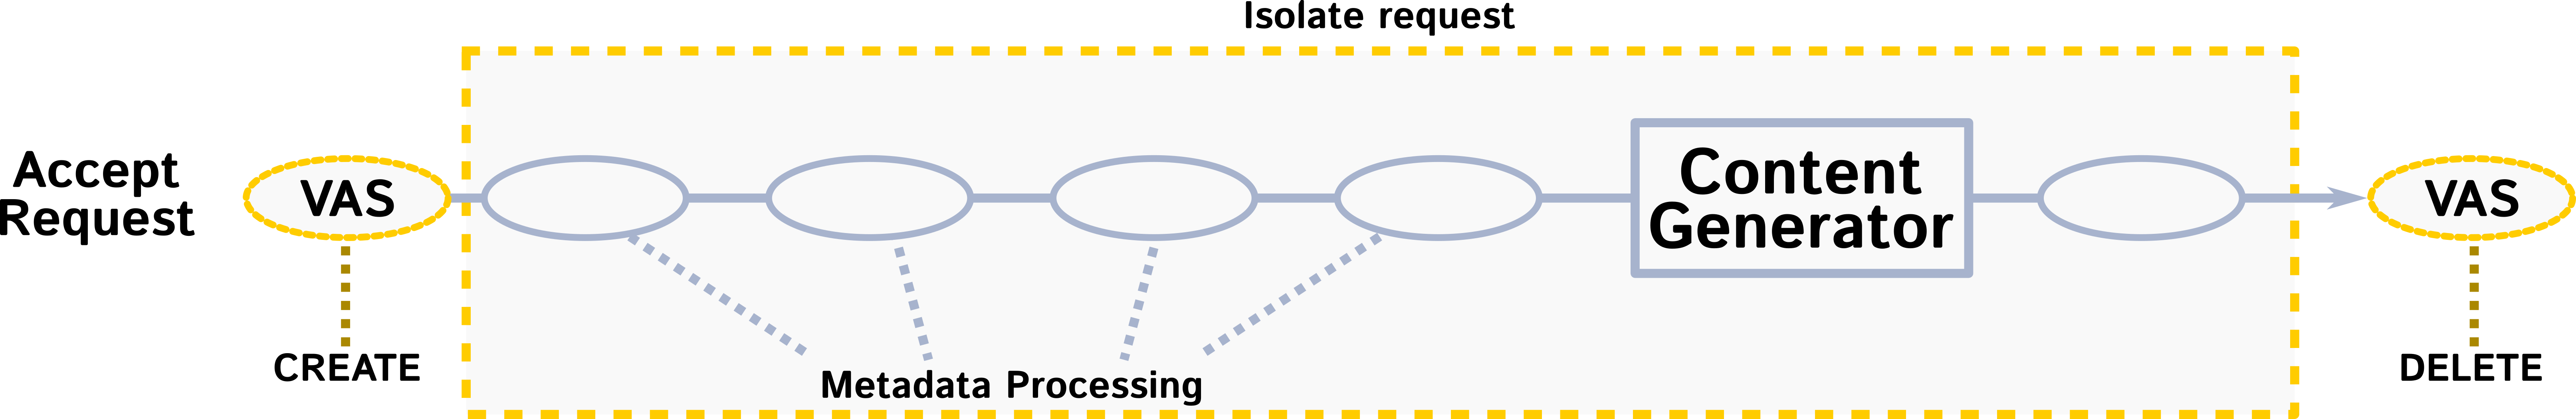
\includegraphics[width=\textwidth]{mvas_httpd}
  
  \caption{httpd com MVAS}
  \label{fig:httpd_mvas}
\end{figure}

A Figura \ref{fig:httpd_mvas} mostra a nossa abordagem para adicionar o MVAS
dentro do httpd. Antes da estrutura de dados da requisição ser construída no
\emph{Apache HTTP Server}, nós temos que criar um novo VAS, anexá-lo na \emph{thread}
atual e mudar para o novo VAS. Depois, todo o ciclo de vida da requisição vai
ser realizada da forma usual, mas dentro de uma nova VAS (totalmente isolado).
Quando uma requisição termina, procedemos com a limpeza das informações
relacionadas ao VAS. Essa abordagem garante o total isolamento de qualquer
requisição.

Nós identificamos as exatas funções que mantém todo o ciclo de vida de um
requisição e aplicamos MVAS para isola-las totalmente uma das outras.
Essas funções são:

\begin{quote}
  \texttt{process\_http\_async\_connection} e\\
  \texttt{ap\_process\_http\_sync\_connection} (ambas localizadas no arquivo
  \texttt{modules/http/http\_core.c})
\end{quote}

Os módulos MPM invocam uma dessas funções para manipular um ciclo de vida de
uma requisição, por esse motivo, adicionar MVAS nessas funções elimina a
complexidade relacionada ao código. Contudo, adicionar o MVAS eleva a
sobrecarga geral para atender as requisições.

O Código \ref{lst:http_core} é um trecho extraído de nossa implementação do MVAS
dentro do \emph{Apache HTTP Server}. Repare que a função \texttt{create\_isolate\_vas()} é
projetada para dar suporte para a criação de uma nova VAS dentro do Apache
HTTP. O código também chama as funções
\texttt{ap\_process\_http\_async\_connection} e
\texttt{ap\_process\_http\_sync\_connection}, ambas isoladas dentro de uma nova
VAS. No começo de cada uma dessas funções é criado uma nova VAS, anexada ao
processo atual e finalmente mudada para uma nova VAS depois que o httpd cria a
requisição. No fim do ciclo de vida, nós removemos a VAS. Nossa implementação
ainda precisa de melhorias, mas já é funcional. Finalmente, todo o código fonte
das nossas modificações está disponível no Github em
\url{https://github.com/LSS-USP/httpd-experiment/commit/aa9e74a3a1157e4345f4bbe977a3e6bd39445e9f}.

\begin{ruledcaption}{Alteração no Apache Server\label{lst:http_core}}
\lstinputlisting[
    language=C,
    ] {code/http_core.c}
\end{ruledcaption}

Esperamos que o MVAS adicione mais latência, contudo, queremos
investigar se a sobrecarga extra é tolerável ou não. O objetivo principal desse
experimento é verificar se o MVAS pode ser utilizado como uma substituição à
estratégia baseada em processos.

\section{Resultados}
\label{sec:preliminary}

O método proposto na Seção \ref{sec:metodologia} busca evidenciar, de forma
clara, sistemática e replicável, as diferenças entre as estratégias baseadas em
processos e \emph{threads}. Por isso, o primeiro passo desses experimentos consiste em
deixar claro a diferença entre as estratégias de MPM, para que em seguida, com
os resultados e a estrutura utilizada, possamos expandir os experimentos para a
versão do Apache que utiliza MVAS.

\subsection{Existe alguma diferença significativa de desempenho entre o apache
HTTP trabalhando com processos e threads?}

Nesse primeiro cenário, temos o httpd com as alterações explicadas na Seção
\ref{sec:customization}, mas sem as modificações do MVAS. Responder essa
pergunta traz vantagens: (1) deixa claro a diferença entre processos e \emph{threads}
no Apache, (2) temos o comportamento base para comparar com o MVAS e (3)
validamos a nossa metodologia.

\begin{table}[h!]
  \centering
  \begin{tabular}{|c|c|c|}
      \hline
    Nome & \textbf{Núcleo} & \textbf{Memória}\\
      \hline
    M1 & 2 & 13Gb \\
      \hline
    M2 & 2 & 4Gb \\
      \hline
   \end{tabular}

  \caption{Hardware}
  \label{tab:machines}
\end{table}



Na Seção \ref{sec:metodologia} e \ref{sec:scenarios}, detalhamos a nossa
metologia e a configuração básica que seguimos. Duas máquinas foram utilizadas,
uma chamada de M1 e a outra de M2 como a Tabela \ref{tab:machines} mostra.
Repare que nós decidimos utilizar apenas alguns núcleos e memórias grandes uma
vez que essas condições são melhores para revelar o comportamento do httpd.

\begin{figure}[!h]
  \centering
  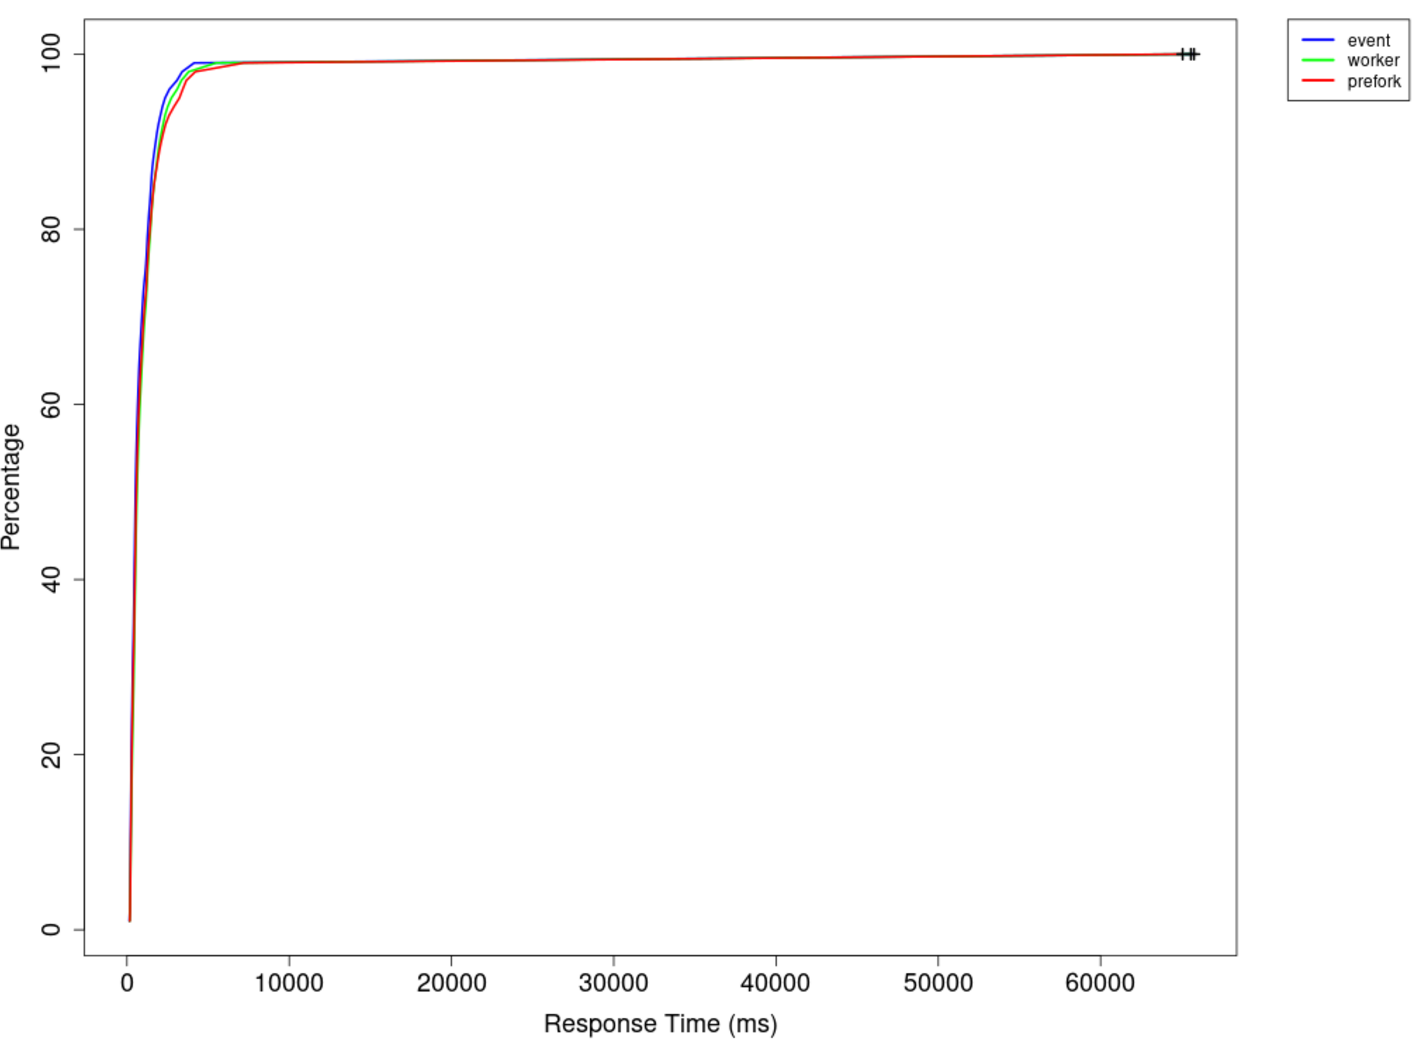
\includegraphics[width=\textwidth]{static_file}

  \caption{Arquivos estáticos: tempo gasto para servir o percentual de requisições}
  \label{fig:static_file}
\end{figure}

O gráfico na Figura \ref{fig:static_file} mostra o percentual de requisições no
eixo y; no eixo x temos o tempo gasto para atender o percentual de requisições
\citep{apache_ab}. A Figura \ref{fig:static_file} mostra o cenário na qual são
servidos arquivos estáticos, recebendo um total de 60000 requisições com até
20000 requisições em paralelo. Além disso, o gráfico ilustra o \emph{Prefork},
\emph{Worker} e \emph{Event} juntos para tornar mais simples de visualizar a
diferença.

\begin{figure}[!h]
  \centering
  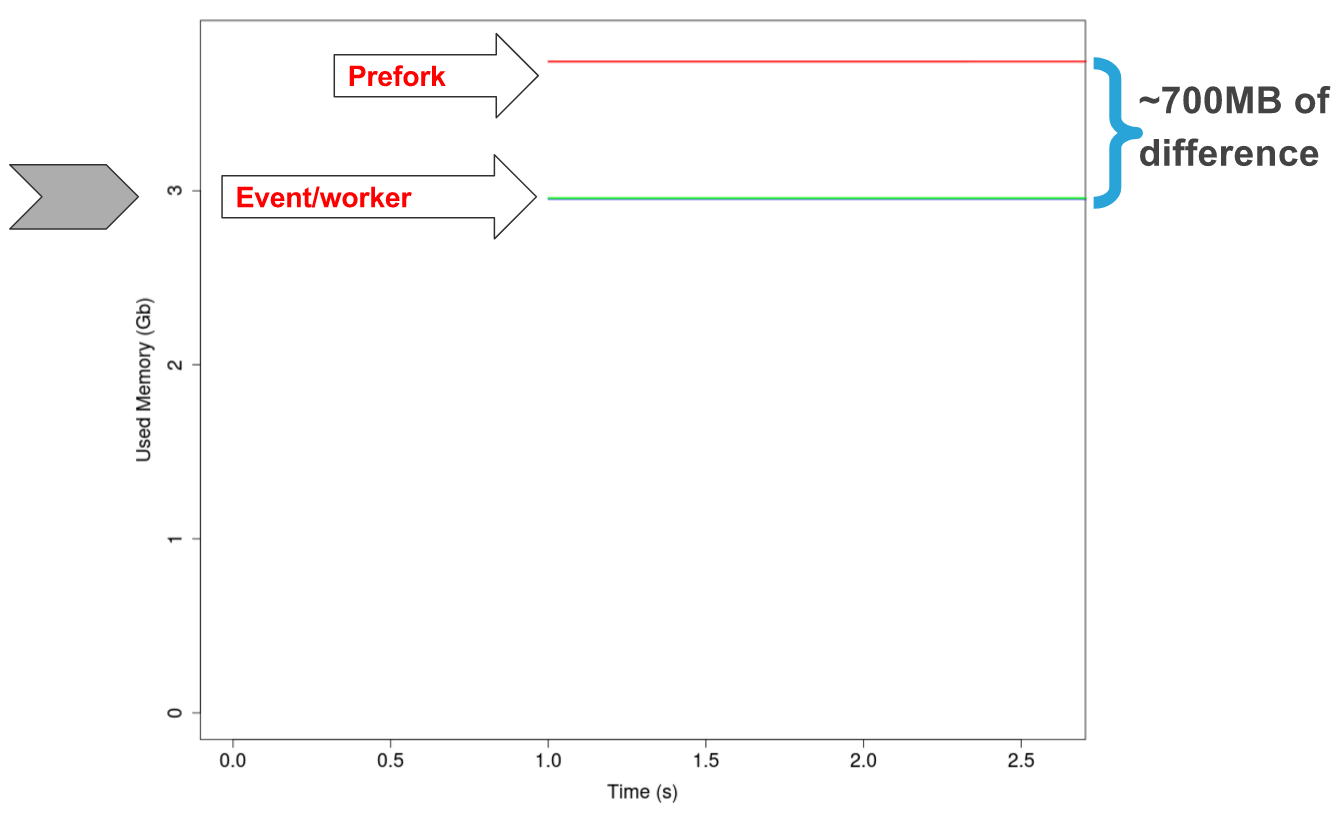
\includegraphics[width=\textwidth]{static_file_memory_usage}

  \caption{Arquivos estáticos: O consumo de memória necessário para atender todas as requisições}
  \label{fig:static_file_memory}
\end{figure}
 
Analisando a Figura \ref{fig:static_file}, é possível perceber que o tempo de
resposta foi praticamente o mesmo para todas as estratégias. Em uma primeira
análise, esse resultado pode parecer frustante uma vez que é de se esperar que
o \emph{Prefork} responda um número menor de requisições. Contudo, a Figura
\ref{fig:static_file_memory} apresenta o mesmo experimento sob a perspectiva do
consumo de memória. Repare que o \emph{prefork} utiliza aproximadamente 3.7Gb e
o \emph{event/worker} precisam de 3Gb para atender a todas as requisições. Esse
resultado evidência uma desvantagem do \emph{prefork} em um cenário simples.
Por fim, é importante ressaltar que um dos motivos de \emph{threads} e
processos terem o mesmo tempo de resposta nesse cenário vem do fato de que a
troca de contexto para \emph{threads} e processos é o mesmo no GNU/Linux
\citep{love}.

\begin{figure}[!h]
  \centering
  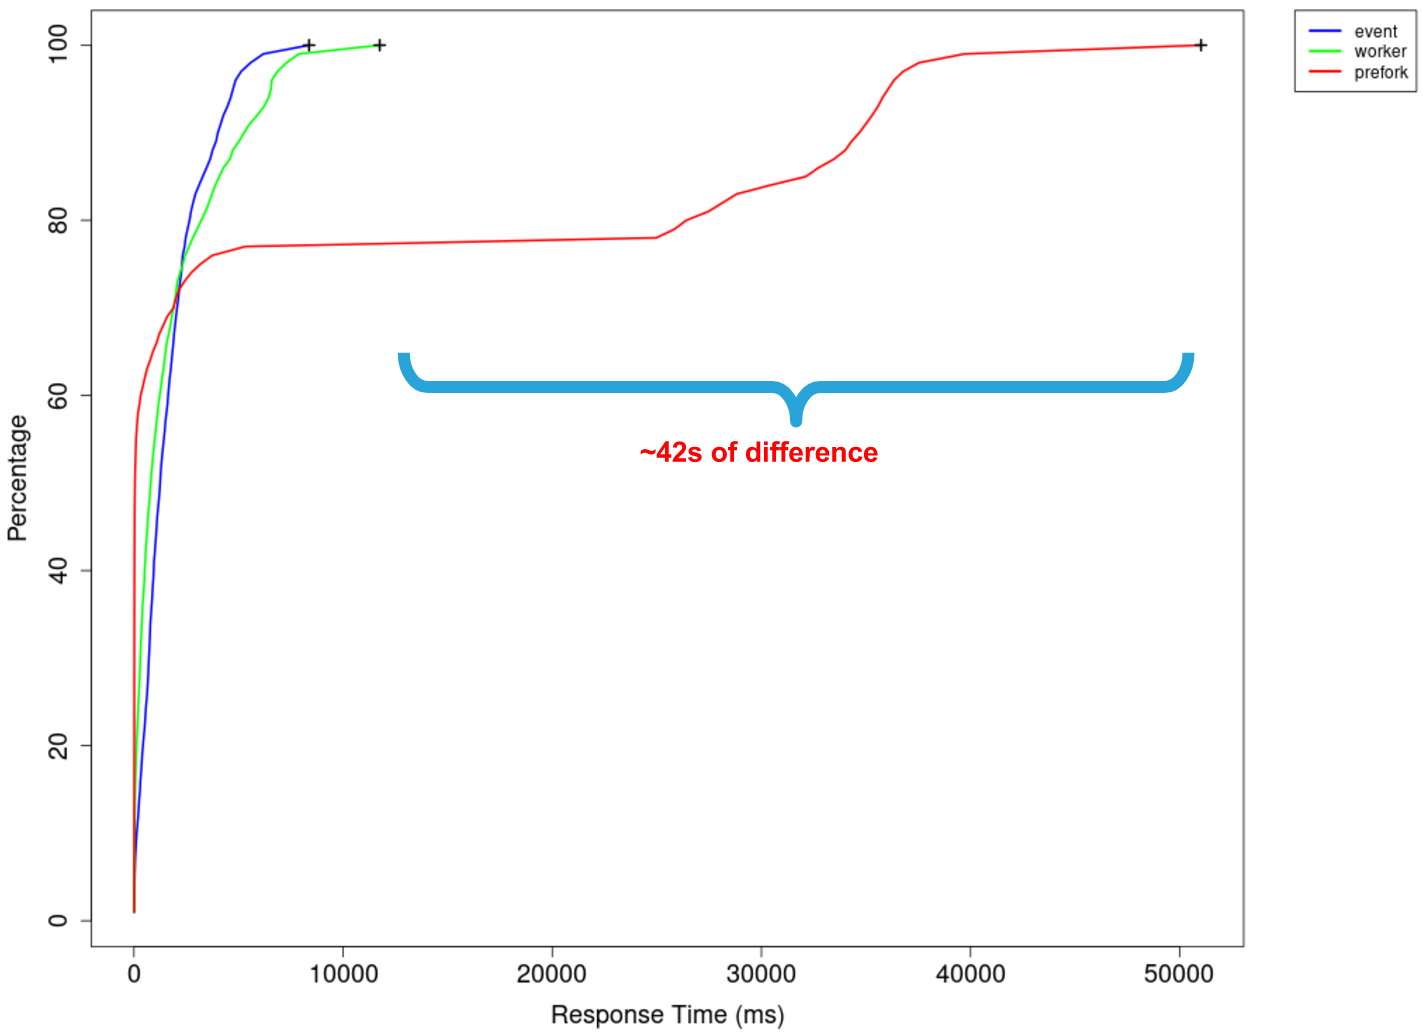
\includegraphics[width=\textwidth]{dynamic_file_request_time}

  \caption{Arquivos Dinâmicos: Tempo gasto por percentual de requisições}
  \label{fig:dynamic_file}
\end{figure}

\begin{figure}[!h]
  \centering
  \includegraphics[width=\textwidth]{dynamic_file_memory_usage}

  \caption{Arquivos Dinâmicos: Consumo de memória necessário para servir as requisições}
  \label{fig:dynamic_file_memory}
\end{figure}

A Figura \ref{fig:dynamic_file} mostra um cenário com arquivos dinâmicos. Nesse
caso, a diferença entre processos e \emph{threads} são muito mais claras. O
\emph{prefork} é mais lento do que o \emph{Event} e \emph{Worker}, a
diferença é próxima de 42 segundos o que é inaceitável em um cenário real.
Para entender melhor esse caso, a Figura \ref{fig:dynamic_file_memory} mostra o
consumo de memória e explicita o enorme gasto de memória do \emph{prefork}
quando comparado com o \emph{Event} e \emph{Worker}. Essa situação pode ser
examinada da perspectiva do SO. Basicamente o Apache tem que criar muitos
processos filhos por requisição e manter eles vivos até que o processamento
termine. Consequentemente, o Apache tem um enorme número de processos vivos e
consumindo memória. Por outro lado, \emph{threads} compartilham dados com os
processos pai, o que reduz o total de memória gasta, assim, mantendo as
\emph{threads} vivas com um custo menor.

Podemos concluir que os experimentos tornam as diferenças claras entre
processos e \emph{threads} dentro do httpd. Os dois cenários descritos são
suficientes para servir como critério para mostrar a diferença entre os MPMs. O
atual resultado fornece informações básicas necessárias para o restante dos
experimentos.

\subsection{Qual a Diferença de Desempenho do Apache Utilizando MVAS Quando
Comparado com as Estratégias Baseadas em Processos e \emph{Threads}?}

A segunda parte das validações tiveram como principais objetivos estudar o
comportamento do kernel Linux com MVAS e com o Apache fazendo uso dos seus
recursos. Como explicado na Seção \ref{sec:mvas_inside_httpd}, já temos a
versão modificada do httpd utilizando MVAS. Instalamos a versão do httpd e
executamos o \emph{benchmark} novamente. Contudo, nossos experimento apontaram
três problemas: (1) MVAS não funciona bem com múltiplas \emph{threads}, (2)
existem problemas de alocação de memória e (3) existe uma enorme sobrecarga nas
operações do MVAS.

Para o primeiro problema, nós conversamos diretamente com o autor do MVAS para
tentar identificar o que estava acontecendo. Depois de várias verificações na implementação,
o autor detectou problemas nas heurísticas de manipulação dos segmentos de
memória.  Basicamente, MVAS tem problemas relacionados a alocação de
pilha. Infelizmente, resolver esse problema requer mudar praticamente
toda a implementação atual do MVAS e essa possibilidade foi, por hora, abandonada.

Para o segundo problema, é preciso recorrer à fundamentação teórica e revisitar
como o Linux aloca memória. Na Seção \ref{sec:visao_pratica_mem} discutimos o
processo de alocação da memória em sistemas Linux e na Figura
\ref{fig:malloc_linux} ilustramos o segmento \emph{heap} para um programa.
Repare da primeira parte da Figura \ref{fig:malloc_linux} que o \emph{heap} é
mapeado para a memória física. Em seguida, o programa pede por mais memória
para o SO por meio da função \texttt{malloc()}. O Linux então estende o tamanho
do \emph{heap} e fornece uma nova referência para a memória imediatamente e
então espera que o programa tente escrever algo na memória.  Assim, depois de
uma tentativa de escrita na memória o kernel realmente aloca memória física
para o programa. Com essa ideia em mente, é possível perceber que o MVAS tem
que manipular esse tipo de situação e esse é um problema complicado para o MVAS
resolver. Infelizmente, o MVAS falha em mapear essa situação e, a cada mudança no
VAS, o SO perde a referência para a memória física.

\section{Discussão Sobre os Experimentos}

Durante a análise das diversas propostas de ampliação das abstrações de
processos, notamos que os dois principais métodos de validação consistem em
utilizar aplicações e \textit{microbenchmarks}. Como já discutimos no Capítulo
\ref{cap:validacoes}, o uso de aplicações é desejável uma vez que elas podem
ser amplamente utilizadas para verificar o impacto geral de uma modificação nas
abstrações de processos. Apesar de vários pesquisadores terem feito uso de tal
abordagem, notamos que nenhum deles realizou experimentos utilizando cargas
expressivas. Por exemplo, os trabalhos que alteraram o Apache realizavam testes
com algumas poucas dezenas de requisições para arquivos estáticos; por exemplo,
o \emph{Light-weight Contexts} faz testes com cargas irrisórias (Vide
Capítulo~\ref{cap:trabalhos-analisados}. Tais testes não evidenciam a real
natureza da alteração feita na abstração de processo pois a aplicação
modificada não é demandada de forma a exercitar o sistema sob pressão.

Esta pesquisa surgiu de uma parceria com a HPe que tinha por objetivo levar o
SpaceJMP para o Linux por meio do MVAS. Para isso era necessário
demonstrar que o MVAS funcionaria bem no Linux. Por isso, ficamos responsáveis
por trabalhar nas validações de tal técnica. Como demostrado ao longo deste
capítulo, tal técnica não é escalável da forma como foi feita. Isso é
interessante de se observar uma vez que tal resultado dialoga com a
argumentação construída no Capítulo \ref{cap:validacoes}; por meio do uso de uma
aplicação real foi demonstrado que uma nova abstração pode não escalar em um sistema real.
Note que esse resultado não significa que desacoplar a VAS é uma ideia ruim,
apenas ilustra que os estudos referentes a tal ideia ainda precisam avançar.

Repare que nos experimentos, nós utilizamos uma abordagem na qual criamos o
nosso \emph{benchmark} do zero; essa decisão foi tomada de forma natural uma
vez que o nosso principal objetivo era inserir o MVAS dentro do Apache.
Contudo, dada a complexidade em se construir
\emph{benchmarks}~\citep{benchrocketscience}, o melhor cenário a longo prazo
consiste na adoção de uma ferramenta bem consolidada de \emph{benchmark}, como
PHORONIX\footnote{\url{https://www.phoronix-test-suite.com/}} ou
LMbench\footnote{\url{http://www.bitmover.com/lmbench/}}.

Durante este trabalho, também buscamos replicar os resultados apresentados pelo
Dune; também colaboramos com os desenvolvedores do Dune por meio do envio de
correções na implementação original deles (\textit{patches}). Os
\textit{microbenchmarks} apresentados pelos pesquisadores comportam-se
perfeitamente como reportado, mas não foi possível replicar os resultados com
as aplicações pois parte do código não estava mais disponível. O Dune é uma das
propostas com maior potencial de ser incorporada nos SOs modernos, contudo a
sua implementação é insegura e não escalável. O principal motivo para isso está
no fato do Dune interceptar os endereços das chamadas de sistemas. Tal
abordagem não funciona desde o momento que o Kernel adotou o sistema de
aleatorização dos endereços de chamadas conhecido por KASLR~\citep{kaslr}.

Portanto, o principal objetivo deste capítulo era apresentar evidências e uma
visão prática da validação de uma nova abstração de processo usando uma
aplicação amplamente conhecida. Além disso, buscamos deixar claro a importância
de utilizar cargas de testes relevantes.

\par

\imgchapter[left]{8cm}{chapter_6_title}{Análise Sobre Abstrações de Processos}
\label{cap:analise-sobre-abstracoes-de-processos}

No Capítulo \ref{cap:trabalhos-analisados}, introduzimos os principais trabalhos
que orbitam em torno de novas abstrações de processos e, a partir de tais
pesquisas, pretendemos desenvolver neste capítulo uma reflexão sobre suas principais
características. Para isso, realizamos diversas análises sobre o estado da arte
da pesquisa em processos e apresentamos um modelo teórico que visa fornecer
uma perspectiva para a nova geração de abstrações de processos. Como resultado,
responderemos as seguintes questões de pesquisa:

\begin{quote}
 \item \textit{QP1:.} ``Quais são as características desejáveis para a próxima geração de abstrações de processos?''
 \item \textit{QP2:.} ``Quais são os principais desafios em se implementar a próxima geração de abstrações de processos?''
\end{quote}

Este trabalho se diferencia dos trabalhos apresentados no
Capítulo~\ref{cap:trabalhos-analisados} por buscar uma visão unificada sobre as
novas extensões nas abstrações de processos e por levar em conta SOs de uso
cotidiano, em especial o GNU/Linux. Esse último critério torna-se relevante
para futuras investigações na área, uma vez que, se tais abstrações alcançarem
SOs de ampla utilização, o impacto e o crescimento da área serão significativos.

\section{Potenciais e Dificuldades Para a Adoção de Novas Abstrações de Processos}
\label{sec:potenciais}
%TODO: Ver a onde da para cortar
Quando a academia faz uma nova proposta para sistemas que estão no ``estado da
prática'', ela deve ser genérica o bastante para ser utilizada por
múltiplas linguagens de programação e deve também considerar questões
referentes a compatibilidade, melhor uso do hardware disponível e
confiabilidade. Assim, apesar dos avanços trazidos pelas pesquisas em SO, elas
estão limitadas às diferentes restrições existentes nos SOs utilizados tanto em
produção quanto em projetos de pesquisa.

SOs usados em produção demandam rigorosa validação para manter o sistema
estável em uma variedade de configurações. Espera-se que um SO maduro busque
prevenir acessos ilegais à memória, impossibilitar a violação de APIs, evitar
consumo excessivo de recursos e impedir erros de sincronização ou
\textit{locking}. Essas características precisam ser garantidas pelo SO
\citep{mondrix}, porém, como esperado, tais restrições dificilmente são
atendidas por propostas de pesquisas devido ao foco dos pesquisadores
em um único problema, desconsiderando assim outros impactos. Por esse motivo,
para que um novo componente sugerido a partir de uma pesquisa acadêmica chegue
aos SOs atuais, é importante garantir que as aplicações que já existem não
sofram impactos negativos em termos de desempenho e de uso.

Outra perspectiva que deve ser considerada é o contínuo desenvolvimento de novos
recursos de hardware. Por exemplo, frequentemente observam-se componentes que
são especializados em um nicho e que, ao longo do tempo, chegam ao usuário
final, tornando-se comuns. Um caso simples que ilustra tal evolução é o
uso de hardware especializado para virtualização, uma vez que esses existiam
apenas para servidores e hoje estão disponíveis para a maioria dos usuários
comuns. Tais recursos representam um novo leque de opções não exploradas,
inclusive possíveis melhorias para as atuais abstrações de processos.

Entretanto, para incorporar novos recursos de hardware à abstração de processos,
não se deve descartar que tal recurso pode não estar disponível para alguns
usuários. Por essa razão, qualquer mudança nos processos para adicionar suporte
a novos recursos de hardware deve levar em consideração todo tipo de situação.
De modo inverso, propostas para melhorar uma abstração de processos podem
sugerir mudanças no hardware e promover avanços no estado da arte dos chips
modernos. Claro que a evolução do hardware necessita de cautela para evitar
quebra de compatibilidade binária com aplicações legadas. Infelizmente, é
preciso ter em mente que as alterações de hardware e suas limitações fazem com
que propostas que dependem de tal evolução sejam difíceis de serem adotadas, e
tornam a ampla adoção de uma determinada melhoria às vezes impraticável.

Algumas das novas abstrações de processos propostas por pesquisadores têm
enorme dependência com outras tecnologias experimentais. Se, por um lado, isso
traz vantagens para as tecnologias em desenvolvimento, por outro, reduz a chance
de adoção de uma nova abstração de processos por um SO de produção devido à
dependência dessa abstração de tecnologias instáveis.

Encontrar um bom balanceamento entre academia e indústria de forma a levar
benefícios para os usuários não é uma tarefa trivial. Nesse sentido, novas
propostas de mudanças na abstração de processos devem considerar as limitações
citadas nessa seção para que possam atender aos requisitos de qualidade
exigidos pelos SOs de uso cotidiano. Infelizmente, afirmar que uma proposta da
academia pode ser adotada ou não pela indústria é uma tarefa complexa dada a
enorme quantidade de variáveis envolvidas em tal análise. Mesmo assim, para
posicionar o leitor em termos do estado da arte e da prática, buscamos
estabelecer um ``potencial de adoção'' de uma nova proposta. Com base nos
critérios apresentados, definimos um conjunto de variáveis que auxilie
na definição das chances de uma pesquisa ser adotada pela indústria:

\begin{enumerate}
  \item
\textbf{Dependência Técnica}: indica se o trabalho é construído
levando-se em consideração outras tecnologias não estabilizadas. Consideramos
tal aspecto um problema para a adoção da nova técnica.

  \item \textbf{Dependência de Compatibilidade}: refere-se às propostas que
exigem alterações na semântica das aplicações em espaço de usuário para que
elas possam tirar proveito de alguma melhoria.

  \item
\textbf{Dependência de Compilador}: propostas que dependem de alterações no
compilador. Nesses casos, consideramos que a adoção torna-se mais complicada
uma vez que dois projetos precisam ser alterados.

  \item
\textbf{Implementação Pesada}: consideramos as implementações pesadas mais
complicadas, uma vez que necessitam realizar mudanças no núcleo do SO, o que
dificulta a adoção.

  \item
\textbf{Implementação Independente}: refere-se a propostas de novas
implementações, claramente de difícil adoção.

  \item
\textbf{Hardware Novo}: indica que a proposta depende de um
hardware novo que só existe em algum contexto específico ou mesmo que ainda não
foi implementado.

  \item
\textbf{Característica Específica de Hardware}: refere-se a propostas de
utilização de algum hardware bem consolidado para algum propósito diferente do
original.

\end{enumerate}

A Tabela \ref{tab:adocao} tenta apresentar o potencial de adoção de cada uma
das propostas citadas no Capítulo \ref{cap:trabalhos-analisados} de acordo com
as variáveis discutidas nesta seção. Na tabela, temos uma marcação indicada
pelo simbolo \ding{54} que significa que uma determinada proposta possui a
limitação indicada na coluna correspondente. Se a proposta não contém tal restrição, então ela
é marcada com o simbolo \ding{52}. Por uma questão de simplicidade, para
definir o potencial de adoção, atribuímos zero para cada \ding{54} e um para
\ding{52}. Por fim, toda vez que a opção ``Hardware Novo'' é marcada,
consideramos que a proposta também requer características específicas de
hardware; para as variáveis referentes à implementação, consideramos que quando
uma proposta parte de uma implementação independente, ela também é considerada
pesada.

\begin{table}[]
\small
\centering

\begin{tabular}{|@{}c@{}|@{}c@{}|@{}c@{}|@{}c@{}|@{}c@{}|@{}c@{}|@{}c|c@{}|@{}c@{}|}
% HEADERS
\hline
  \multirow{2}{*}{Trabalho}          &
  \multicolumn{3}{c|}{Dependência}   &
  \multicolumn{2}{c|}{Implementação} &
  \multicolumn{2}{c|}{Hardware}       &
  \multirow{2}{*}{Adoção} \\ \cline{2-8} &
      Técnica & Compatibilidade & Compilador & Pesada & Independente &
      \multicolumn{1}{c|}{Novo} & Característica &
\\ \hline
%           Técnica     Compatib    Compilaca   Pesada      Independente                     Novo        Caracact   Adocao
Dune      & \ding{54} & \ding{54} & \ding{54} & \ding{54} & \multicolumn{1}{c|}{\ding{54}} & \ding{54} & \ding{52} & \\ \hline
Shreds    & -- & -- & -- & \ding{54} & \multicolumn{1}{c|}{--} & -- & -- & \\ \hline
Wedge     & \ding{54} & \ding{52} & \ding{52} & \ding{52} & \multicolumn{1}{c|}{\ding{54}} & \ding{54} & \ding{54} & \\ \hline
\begin{tabular}[c]{@{}c@{}}Resource\\ Container\end{tabular} & & & & & \multicolumn{1}{c|}{} & & & \\ \hline
Nooks     & \ding{54} & \ding{52} & \ding{54} & \ding{52} & \multicolumn{1}{c|}{\ding{54}} & \ding{54} & \ding{54} & \\ \hline
Mondrian  & -- & -- & -- & -- & \multicolumn{1}{c|}{ -- } & -- & -- & \\ \hline
SpaceJMP  & \ding{54} & \ding{52} & \ding{52} & \ding{52} & \multicolumn{1}{c|}{\ding{54}} & \ding{54} & \ding{54} & \\ \hline
LwC       & \ding{54} & \ding{52} & \ding{54} & \ding{52} & \multicolumn{1}{c|}{\ding{54}} & \ding{54} & \ding{54} & \\ \hline
Exokernel & -- & -- & -- & -- & \multicolumn{1}{c|}{--} & -- & -- & \\ \hline
\end{tabular}

\caption{Potencial de adoção}
\label{tab:adocao}

\end{table}


\section{Extração de Conceitos Derivados das Pesquisas em Abstrações de Processos}
\label{sec:extracao}

Todas as pesquisas apresentadas no Capítulo \ref{cap:trabalhos-analisados}
configuram o estado da arte no que se refere às abstrações de processos.
Infelizmente, nenhuma delas encontra-se no código principal de qualquer SO de
uso cotidiano. Parte desse problema vem dos fatos apresentados anteriormente na Seção
\ref{sec:potenciais}, contudo outros aspectos que contribuem para que tais
propostas não estejam presentes nos SO modernos vêm da falta de unificação e
sistematização de tais ideias. Ao analisar cada uma das propostas, notamos que
todas elas propõem direta ou indiretamente algum nível de desacoplamento entre
os elementos presentes no SO. Tal observação nasce da abordagem radical tomada
pelos criadores do Exokernel, que levaram o nível de desacoplamento do SO ao
extremo. Apesar do Exokernel ser um sistema de difícil adoção em termos
práticos, ele nos alerta sobre as vantagens da redução de dependências
entre os elementos do SO e as possibilidades que ela pode levar ao espaço de
usuário. Tendo isso em mente, revisitamos de forma breve alguns dos trabalhos
apresentados no Capítulo \ref{cap:trabalhos-analisados} sob a ótica do
desacoplamento e seus potenciais benefícios.

Iniciamos analisando o projeto Dune. Esse projeto traz uma nova perspectiva de uso dos recursos de virtualização
disponibilizados pelas CPUs modernas que, consequentemente, traz dois
benefícios diretos: otimização e flexibilidade. Ao utilizar os recursos de
virtualização para acelerar certas tarefas, o Dune promoveu avanços em um setor
difícil de ser otimizado. Além disso, tais melhorias facilitam certas
implementações no espaço de usuário, pois removem a necessidade de códigos com
técnicas avançadas que visam trazer melhorias de desempenho; em outras
palavras, a proposta do Dune pode melhorar a legibilidade de alguns códigos.
Os avanços citados foram factíveis graças ao \textbf{desacoplamento da
virtualização}, que possibilita entregar melhorias de desempenho no
espaço de usuário de maneira relativamente simples (do ponto de vista da
aplicação) e também fornece ganhos de segurança.

Já o projeto Nooks se distancia um pouco da abstração de processos, uma vez que
busca tornar o núcleo do SO mais resiliente. Contudo, ao criar mecanismos
que reagem de forma a reduzir as chances de o sistema quebrar, tal proposta
apresenta o \textbf{desacoplamento dos recursos}, de forma a fornecer mecanismos
para que os processos possam se recuperar ou tomar ações em casos de falhas.
Adicionalmente, essa técnica cria um interessante mecanismo de
comunicação entre as extensões do Kernel e os seus drivers, permitindo que o SO
se ``defenda'' de problemas que ocorram com um código que foi acoplado ao seu
núcleo.

De forma mais direta e sistemática, o \textit{Resource Container} sugere o
controle fino do gerenciamento de recursos e consequentemente o
\textbf{desacoplamento do gerenciamento de recursos} de tal elemento. De certa
maneira, essa proposta já pode ser encontrada incorporada nos SOs atuais, sob a
forma de contêineres no Linux, mais especificamente, como o
\textit{cgroups}\footnote{\emph{cgroups} é uma funcionalidade fornecida pelo
Linux que permite limitar e isolar recursos de uma coleção de processos.}. A
principal contribuição do do \emph{Resource Container} vem da sua capacidade de permitir que a
própria aplicação tome conta da sua execução.  Ainda que parte das ideias
apresentadas por esse trabalho estejam presentes em alguns SOs, as
implementações ainda são relativamente reduzidas em termos do escopo
apresentado na pesquisa.

Uma abordagem alternativa que visa atender uma nova geração de computadores com
memórias não voláteis na ordem dos petabytes é o SpaceJMP/MVAS.  Os autores
sugerem o \textbf{desacoplamento do VAS dos processos} e permitir que eles tenham
múltiplos VAS e, de forma reativa, a aplicação torne-se capaz de mudar o VAS
atual. Essa abordagem faz com que um processo consiga acessar regiões muito
maiores do que aquelas garantidas pelo tamanho de um VAS. Indiretamente,
desacoplar um VAS adiciona a possibilidade de criar processos persistentes,
isto é, que vivem mesmo após o reboot ou mesmo após um problema. Desacoplar o VAS
pode trazer benefícios para aplicações de \textit{checkpoints}, melhorar o
gerenciamento de bibliotecas, e elevar o nível de isolamento e compartilhamento.

O projeto  Light-weight Context (lwC) indiretamente propõe o total
\textbf{desacoplamento do PC}; vale observar que os autores explicitam outros
desacoplamentos, contudo, para esse trabalho, acreditamos que o desacoplamento
do PC é o que melhor descreve as inovações propostas. Desacoplar o PC leva uma
infinidade de possibilidades para o espaço de usuário, uma vez que o processo
pode fazer operações semelhantes às do escalonador sem grandes custos e dentro
do mesmo intervalo de execução do processo. lwC tem como principal
característica um robusto e interessante modelo de programação que permite
às aplicações no espaço de usuário utilizarem novos paradigmas de desenvolvimento.
Isso cria diversas oportunidades para desenvolver novos tipos de manipulações,
tal como criar \emph{snapshots} do estado atual do processo e depois reverter o
processo para o estado anterior. Dado os múltiplos \emph{snapshots}
(contextos), é possível fazer com que um processo em execução mude para uma
outro contexto com diferentes restrições de acesso a memória permitindo isolar
trechos de código sensível.  Ao contrário do que parece, isso não é como
utilizar \emph{threads} ou processos independentes. Por não haver dependência
do escalonador para mudar o contexto do processo (o que é razoavelmente caro),
a própria aplicação pode escolher quando e qual contexto manipular e fornecer,
assim, um controle fino para os programadores (o que pode melhorar o desempenho
e a segurança).

De modo geral, percebemos que vários dos trabalhos analisados têm preocupação com o gerenciamento e acesso a
memória; em especial, vários deles questionam o tratamento dado à memória pelos
SOs atuais.  A abordagem de utilizar um único espaço de endereçamento por
processo tem se provado eficiente ao longo dos anos, porém, apesar do seu
sucesso, essa não é uma abordagem à prova de falhas e ainda carece de
melhorias. Primeiramente, a abordagem de isolar os processos por meio do
espaço de endereçamento linear melhora a confiabilidade do sistema e a
segurança. Entretanto, um processo não tem uma forma de restringir o seu próprio
acesso ao seu segmento de memória, o que pode ser útil para reduzir os riscos de
falhas de segurança ocasionados por binários de terceiros. Em segundo lugar, o
controle do compartilhamento de memória acontece no tamanho de uma página e
cria a oportunidade para explorar falhas, tais quais \emph{buffer e stack
overflow} ou mesmo o compartilhamento de bibliotecas comprometidas. Com essa preocupação, os
trabalhos Wedge, shreds e mondrix/mondrian buscam trazer melhorias para essas fragilidades.

Analisando as abstrações de processos da perspectiva da segurança, o projeto
Wedge retoma uma antiga premissa que defende o princípio do menor privilégio.
Ela afirma que precisamos mudar a lógica atual de conceder permissão por
padrão para uma ideia de negar permissão por padrão. Essa mudança de paradigma
torna supostamente possível a redução das chances de ataques e vazamento de
dados, uma vez que o programador precisa indicar explicitamente o que será
exposto. Tal pesquisa indiretamente propõe o \textbf{desacoplamento dos
privilégios} da abstração de processos. Além disso, ela mantém a
compatibilidade entre aplicações novas e legadas, sendo uma opção de uso ao programador.

Entrando um pouco mais nas questões de proteção e controle-fino da memória,
destacamos o shreds e o mondrix/mondrian. shreds nasce com a ideia de evitar
ataques conhecidos como abusos intra-processos de conteúdo da memória. Os
autores defendem que o acesso a certas regiões da memória de um processo
que esteja executando em espaço de usuário merecem proteção especial. Em tal proposta, os
autores utilizaram um recurso específico dos processadores ARM em conjunto com
um mecanismo de gerenciamento da região de memória (Seção
\ref{sec:outros_mecanismos_memoria}). Essa proposta entrega mais flexibilidade,
segurança e controle ao acesso da memória.

Na mesma linha de fornecer controle fino sobre a memória, os autores do Mondrix
propuseram, de forma mais radical, um mecanismo de controle do acesso à memória
no nível das palavras de dados. Para isso, os autores sugerem alterações no
hardware e no SO de forma a controlar todo acesso com a menor granularidade
possível. Indiretamente, shreds e mondrix são propostas de
\textbf{desacoplamento do controle de memória}.

\section{Bead: Um Modelo Teórico Para a Próxima Geração de Abstrações de Processos}
\label{sec:bead}

Neste trabalho discutimos as abstrações de processos partindo do conhecimento
já estabelecido e consolidado pela indústria até chegar ao estado da arte de
novas propostas para melhorar o conceito de processo. Durante toda a pesquisa,
percebemos que as diversas propostas giram em torno do desacoplamento de
elementos do processo, contudo, não existe uma tentativa de organizar as
diversas ideias propostas. Nesse sentido, observamos e analisamos diferentes propostas de
desacoplamento que representam o estado da arte, acreditando que várias
das ideias apresentadas podem atingir o ``estado da prática'' e assim pavimentar
novos ramos de pesquisas. Como resultado dessa pesquisa, compilamos os diversos
trabalhos estudados em um modelo que busca elevar o grau de desacoplamento
dentro das abstrações de processos.

Para exemplificar a proposta de desacoplamento deste trabalho, faremos uma
analogia com a evolução do modelo atômico. Começamos por um dos primeiros
modelos atômicos aceitos pela comunidade científica, proposto por Dalton, que
afirmava que um átomo era uma esfera maciça e indivisível. Em seguida, Thomson
propôs outro modelo no qual os átomos eram compostos por partículas positivas e
negativas, o que indicava a divisibilidade dos átomos. Posteriormente, Rutherford
refinou o modelo, propondo um esquema em que o átomo possui um núcleo e os
elétrons giram em torno desse núcleo formando um sistema semelhante ao modelo
planetário. O modelo atômico continua sendo evoluído e sofisticado, contudo a principal lição que tiramos disso para o nosso contexto é o
constante refinamento do modelo e os avanços que vêm junto com ele.

Seguindo a analogia do modelo atômico, podemos considerar que as abstrações de
processos estão em um estágio equivalente ao modelo de Thomson. A abstração de
processo não é mais um bloco sólido e indivisível; ela possui um leve grau de
desacoplamento, uma vez que no passado notou-se a vantagem em se desacoplar o PC
e a Pilha, possibilitando múltiplos fluxos de execução no mesmo processo
(\emph{threads}). Seguindo esse raciocínio e buscando avançar o modelo atual,
apresentamos o modelo \textbf{bead}\footnote{\emph{Bead} em inglês,
refere-se às pequenas contas que compõem um colar ou pulseira. Normalmente,
existe uma ampla variedade de tais objetos.} que consiste em buscar um elevado
grau de desacoplamento dos elementos da abstração de processos.


\begin{table}[]
\small
\centering
  \begin{tabular}{|@{}c@{}|@{}l@{}|@{}l@{}|@{}l@{}|@{}l@{}|@{}l@{}|@{}l@{}|}
  % TOPO DA TABELA
  % |M{2.5cm}|M{2.5cm}|M{2.5cm}|
  \hline
  \multicolumn{1}{|l|}{\diagbox[width=2.5cm, height=2cm]{Desacoplar}{Vantagem}} &
    % Troca de contexto
    \multicolumn{1}{@{}c@{}|}{\begin{tabular}[c]{@{}c@{}}Troca de\\ Contexto \\no Espaço\\ de Usuário\end{tabular}} &
    % Persistência de processos
    \multicolumn{1}{@{}c@{}|}{\begin{tabular}[c]{@{}c@{}}Persistência\\ de processos\end{tabular}} &
    % Controle fino de privilégios
    \multicolumn{1}{@{}c|}{\begin{tabular}[c]{@{}c@{}}Controle \\fino de \\ privilégios\end{tabular}} &
    % Segurança
    \multicolumn{1}{@{}c|}{Segurança} &
    % Recuperação
    \multicolumn{1}{@{}c|}{Recuperação} &
    % Otimização
    \multicolumn{1}{@{}c|}{Otimização} \\ \hline
  % Início da tabela
  PC                                                                    &                             & & & & & \\ \hline
  \begin{tabular}[c]{@{}c}Isolamento \\de memória\end{tabular}          &                             & & & & & \\ \hline
  VAS                                                                   &                             & & & & & \\ \hline
  \begin{tabular}[c]{@{}c}Resource\\ Management\end{tabular}            & \ding{52}\ding{52}\ding{52} & & & & & \\ \hline
  \begin{tabular}[c]{@{}c}Controle de\\ acesso a\\ memória\end{tabular} &                             & & & & & \\ \hline
  Virtualização                                                         &                             & & & & & \\ \hline
  Privilégios                                                           &                             & & & & & \\ \hline
  \end{tabular}
\caption{Relação desacoplamento beneficio}
\label{tab:desacoplamento_beneficio}
\end{table}


Como apresentado na Seção \ref{sec:potenciais}, para que os desacoplamentos
propostos nas pesquisas sejam absorvidos pelos SOs atuais é preciso considerar
diversos aspectos. Em especial, destacamos que as abordagens que seguem uma
implementação leve e que atendem as propostas de desacoplamento destacadas na
Tabela \ref{tab:desacoplamento_beneficio} são preferíveis. Essa tabela mostra as
propostas de desacoplamento na vertical e os benefícios que elas podem trazer
aos SOs. Por fim, utilizamos uma escala de zero a três \ding{52}, que indica o
quanto de benefício um determinado desacoplamento pode levar para uma área.

\begin{figure}[!h]
  \centering
  \includegraphics[width=\textwidth]{decomposicao_overview}
  \caption{Decomposição do processo}
  \label{fig:decomposicao_proc}
\end{figure}

A Figura \ref{fig:decomposicao_proc} busca mostrar de forma visual o modelo de
abstração de processos proposto por este trabalho. Na parte central da figura
temos os três elementos fundamentais para o uso dos processos: PC, Pilha e
contexto de E/S. Nas camadas mais externas temos o VAS, que é um elemento
importante para que os processos em SOs de propósito geral funcionem de forma
apropriada (dada sua importância, ele ocupa boa parte da representação da
abstração).  Em seguida notamos diversos elementos que orbitam a abstração
atual de processos. Eles podem ser vistos como elementos menos importantes para
o correto funcionamento da abstração, mas são fundamentais para diversas
aplicações modernas. Note na Figura a presença de ``??'', esse foi inserido na
imagem com o objetivo de simbolizar outros desacoplamentos que não detectamos
ou que venham a surgir no futuro. Por fim, no canto direito da figura,
destacamos apenas os dois principais elementos envolvidos na criação das
\emph{threads}; repare que \emph{threads} podem ser vistas como desacoplamentos
do PC e da pilha.

\subsection{A API Bead}
\label{sec:api}

Nesta subseção discutiremos a proposta de API do \emph{Bead}, que tem por
objetivo fornecer uma visão do funcionamento desse modelo; note que a
implementação do \emph{Bead} consiste em um trabalho futuro. Em termos de API e
implementação, queremos manter os critérios para adoção descritos na Seção
\ref{sec:potenciais} e, ao mesmo tempo, fornecer uma API unificada que possa
ser utilizada no espaço de usuário. Para que tal modelo possa ser implementado,
é preciso usar uma abordagem que caminha entre uma implementação estrutural
leve e pesada.  Implementação pesada significa que será necessário inserir
códigos intermediários nas atuais abstrações de processo para que esses
forneçam mecanismos externos e permitam às extensões atuar sobre o núcleo do
SO. Tal abordagem visa manter a compatibilidade com as aplicações já existentes
sem forçar mudanças nas aplicações no espaço do usuário. Implementação leve é
quando queremos o maior grau de desacoplamento possível como também facilidade
para futuras expansões no modelo.

Como mostrado no Capítulo \ref{cap:trabalhos-analisados}, cada proposta de
extensão na abstração de processo sugere uma API para o seu contexto
específico. Nesse sentido, buscamos aprender as técnicas utilizadas pelos
trabalhos anteriores e combinamos as principais chamadas dentro do bead. A
seguir, apresentamos as operações fornecidas, uma breve descrição sobre o seu
comportamento e o trabalho do qual foi derivada. Observe que o conjunto dessas
operações pode ser abstraído para uma biblioteca no espaço do usuário e que a
combinação das várias operações possibilita a criação de novos modelos de
programação (discutiremos padrões de utilização na próxima seção). 

\begin{description}
  \item [\texttt{BEAD\_SET\_CONFIG}:]

Essa operação atua diretamente nas configurações referentes às abstrações de
processos. Ela espera que o programa indique explicitamente quais
desacoplamentos utilizar. Se nenhuma informação for passada, assume-se um
conjunto de configurações padrão compatível com a maioria das aplicações
atuais. As configurações do que será desacoplado são feitas por meio desse comando.

  \begin{itemize}
    \item \textbf{Parâmetros:}

Espera uma estrutura de dados padrão que encapsula todas as informações
referentes aos desacoplamentos desejados.

    \item \textbf{Retorno:}

Se todas as configurações solicitadas pelo usuário forem suportadas, então a
função devolve o status 0. Se alguma das operações falhar, o status é um valor
positivo construído por meio de manipulações binárias na qual cada bit
significa uma falha que ocorreu\footnote{Definir o significado para cada bit,
representa um nível de detalhe que pode varia de SO para SO. Por isso, não
especificamos tais valores.}. 

    \item \textbf{Referência:}

Essa operação surge da necessidade de unificar as diversas propostas, por isso
não tem referência direta a nenhum trabalho.

  \end{itemize}

  \item [\texttt{BEAD\_GET\_CONFIG}:]

Essa operação atua recuperando as configurações referentes às abstrações de
processos. 

  \begin{itemize}
    \item \textbf{Parâmetros:}

Espera uma estrutura de dados padrão que será utilizada para preencher as
informações.

    \item \textbf{Retorno:}

Devolve 0 se tudo ocorrer como esperado, ou um valor negativo de status de
erro.

    \item \textbf{Referência:}

Operação criada no contexto deste trabalho.

  \end{itemize}

  \item [\texttt{BEAD\_NEW\_CONTEXT\_INSTANCE}:]

Essa chamada comporta-se de forma similar ao \texttt{fork()}, pois
faz uma cópia idêntica dos elementos do processo pai, porém diferencia-se dela
por não criar uma nova \emph{thread} e
compartilhar o mesmo PID do processo pai. Na prática, essa função também pode
receber alguns parâmetros que alteram o seu comportamento padrão.

  \begin{itemize}
    \item \textbf{Retorno:}

Se estiver no processo que invocou a operação, então um descritor do novo
contexto é retornado. Caso contrário, se estiver dentro de um contexto criado,
retorna -1.

    \item \textbf{Referência:}

Chamada baseada em \texttt{lwCreate()}, proposta pelo lwC.

  \end{itemize}

  \item [\texttt{BEAD\_SWITCH}:]

Dentre as operações mais comuns observadas nos diversos trabalhos, destaca-se o
mecanismo de troca de alguma propriedade dentro do processo. Nesse contexto, a
operação \texttt{BEAD\_SWITCH} unifica operações de mudanças dentro do
processo. Destacam-se os casos da troca de contexto e de entrada em regiões
mais seguras da memória. A operação pode esperar um descritor que referencia uma
instância de um contexto que seja válida. Com base no descritor recebido, essa
chamada transfere a \emph{thread} de execução do processo que invocou tal chamada para
a instância de contexto criada anteriormente. Outra utilização dessa operação é
a troca da execução de uma área menos segura para outra mais segura por meio da
operação \texttt{BEAD\_ENTER\_CONTEXT}.

  \begin{itemize}
    \item \textbf{Parâmetros:} 

    \begin{itemize}
      \item \texttt{Descriptor}: Descritor do contexto alvo
    \end{itemize}

    \item \textbf{Retorno:}

Se algo der errado, essa função devolve um valor negativo informando o erro.

    \item \textbf{Referência:}

Chamada baseada em \texttt{lwSwitch()}, proposta pelo lwC.

  \end{itemize}

  \item [\texttt{BEAD\_VIRTUALIZATION\_MODE}:]

A chamada para essa operação faz com que o processo entre em modo de
virtualização, i.e., faz uso dos recursos de virtualização disponíveis. Essa função pode ter o seu comportamento alterado via parâmetro ou via
configurações externas. Dentre as possíveis configurações, encontra-se a
possibilidade de restringir qual operação de virtualização deseja-se utilizar.

  \begin{itemize}
    \item \textbf{Parâmetros:}

    \begin{itemize}
    \item \texttt{Options}: Recebe opções que determinam o modo de virtualização.
    \end{itemize}

    \item \textbf{Retorno:}

Se algo der errado, essa função devolve um valor negativo informando o erro.

    \item \textbf{Referência:}

Chamada baseada em \texttt{dune\_entry()}, do Dune.

  \end{itemize}

  \item [\texttt{BEAD\_ENTER\_COMPARTMENT}:]

Essa operação faz com que a \emph{thread} em execução tenha associado a si um
compartimento ao qual apenas ela tem acesso. Isso auxilia contra
ataques intra-processos. Nenhuma outra \emph{thread} do processo tem acesso a qualquer
dado do compartimento e o mesmo vale para os dados dentro do compartimento
(i.e., o compartimento é isolado). Devido ao isolamento oferecido por essa
técnica, torna-se necessária uma função especial para realizar a alocação de memória
dentro do compartimento. Essa operação trabalha em conjunto com a operação
\texttt{BEAD\_SWITCH}.

  \begin{itemize}
    \item \textbf{Retorno:}

Devolve 0 se tudo ocorrer bem, ou um código de erro se algo der errado.

    \item \textbf{Referência:}

Chamada baseada em \texttt{shred\_enter()}, proposta pelo Shred.

\end{itemize}

  \item [\texttt{BEAD\_EXIT\_COMPARTMENT}:]

Essa função sai do compartimento atual.

  \begin{itemize}

    \item \textbf{Retorno:}

Devolve 0 se tudo ocorrer bem, ou um código de erro se algo der errado.

    \item \textbf{Referência:}

Chamada baseada em \texttt{shred\_exit()}, proposta pelo Shred.

  \end{itemize}

  \item [\texttt{BEAD\_ALLOC\_COMPARTMENT}:]

Essa operação é responsável por alocar memória dentro de um compartimento e tem
o seu funcionamento similar ao da função \texttt{malloc()}. Uma vez que a
memória é alocada utilizando essa operação, ela é acessível
apenas dentro da \emph{thread} que solicitou entrar no compartimento. Esse mecanismo
de isolamento de memória faz com que as páginas do próprio processo tenham o
seu acesso restrito a uma \emph{thread}.

  \begin{itemize}
    \item \textbf{Parâmetros:}

    \begin{itemize}
      \item \texttt{tamanho}: Tamanho em bytes que se deseja alocar.
    \end{itemize}

    \item \textbf{Retorno:}

Devolve um ponteiro para a região de memória alocada. Em caso de erro, o valor
NULL é devolvido.

    \item \textbf{Referência:}

Chamada baseada no Shred.

  \end{itemize}

  \item [\texttt{BEAD\_FREE\_COMPARTMENT}:]

A operação de liberar o compartimento alocado simplesmente reverte a operação
feita por \texttt{BEAD\_ALLOC\_COMPARTMENT}.

  \begin{itemize}
    \item \textbf{Parâmetros:}

    \begin{itemize}
      \item \texttt{Ref}: Ponteiro para a memória previamente alocada.
    \end{itemize}

    \item \textbf{Retorno:}

Não devolve nada.

    \item \textbf{Referência:}

Chamada baseada no Shred.

  \end{itemize}
%  \item [\texttt{BEAD\_REGISTER\_TRANSFER\_CONTROL}:]
%  \item [\texttt{BEAD\_REGISTER\_TRANSFER\_ENTRY}:]
%  \item [\texttt{BEAD\_NEW\_EXECUTION\_CONTEXT}:]
\end{description}

\subsection{Padrões de Utilização}
\label{sec:padroes}

As operações indicadas na Seção~\ref{sec:api} podem ser entendidas como funções
ou constantes utilizadas para determinar o procedimento que deve ser
feito\footnote{Entendemos que tal decisão deve ser tomada pelo próprio
desenvolvedor.}. Para manipular as diversas operações fornecidas pelo
\emph{bead}, utilizaremos uma função central (\texttt{beadctl()}) responsável
por gerenciar as chamadas de sistema solicitadas pelo usuário. Essa função
receberá dois valores como parâmetro: (1) uma constante representando a
operação do \emph{bead} solicitada e (2) uma estrutura de dados padronizada
(\texttt{bead\_data}). O \texttt{beadctl()} atua de forma seletiva sobre as
operações solicitadas como pode ser visto no Pseudocódigo~\ref{alg:ctlbead} --
ao longo deste capítulo, adotaremos essa função como padrão. Note que ela se
comporta como um adaptador chamado no espaço de usuário e que, por sua vez, faz
o pedido direto para o Kernel (essa função é análoga ao IOCTL presente no
Linux).

\begin{pseudocode}

\begin{lstlisting}[language=pseudocode, style=pseudocode]
function beadctl(code, data)
  ret $\gets 0$
  switch(code)
    case BEAD_SET_CONFIG:
      bead_set_config(data)
      break
    case BEAD_GET_CONFIG:
      break
    case BEAD_NEW_CONTEXT_INSTANCE:
      ret $\gets$ bead_ctx_instance(data)
      break
    case BEAD_SWITCH:
      ret $\gets$ bead_ctx_switch(data)
      break
    case BEAD_VIRTUALIZATION_MODE:
      ret $\gets$ bead_virtualization(data)
      break
    case BEAD_ALLOC_COMPARTMENT:
      break
    case BEAD_FREE_COMPARTMENT:
      break
    case BEAD_ENTER_COMPARTMENT:
      break
    case BEAD_EXIT_COMPARTMENT:
      break
    default:
      break

  return ret

\end{lstlisting}

  \caption{Função de controle das propriedades do \emph{bead}}
  \label{alg:ctlbead}
\end{pseudocode}


Para passar dados do espaço de usuário para o kernel (e vice-versa), definimos
uma estrutura de dados para realizar a troca de informações de forma
padronizada. O Pseudocódigo~\ref{alg:beadata} ilustra uma potencial estrutura
de dados para realizar a troca de informação do espaço de usuário para o kernel.
Note que essa estrutura de dados nasce com o objetivo de simplificar as
chamadas de função, unificar as diferentes propostas e a facilitar a
comunicação.

\begin{pseudocode}

\begin{lstlisting}[language=pseudocode, style=pseudocode]
struct bead_data {
  enable_recursive_snapshot, // Total de fotografias recursivas, falso por padrão
  max_snapshot_level, // Total de fotografias recursivas
  total_of_snapshot, // Total de fotografias tiradas
  ctx_ids[], // Estrutura de dados contendo as referências para os ids
  vitualization_flags, // Conjunto de flags de controle sobre quais recursos oferecer para o processo
  vas_flags, // Conjunto de flags utilizada para controlar o desacoplamento da VAS
  switch_option, // Flags de configuração feita sobre a troca
  compartments, // Flags de configuração do compartimento
  compartmentS_size, // Tamanho de um compartimento
}

\end{lstlisting}

  \caption{Estrutura de dados utilizada pelo bead para troca de dados do espaço de usuário com o de kernel (vice-versa)}
  \label{alg:beadata}
\end{pseudocode}


Introduzimos nesta seção alguns dos possíveis padrões de utilização do
\emph{bead}. Nosso objetivo é ilustrar como tal API pode levar benefícios para
as aplicações, principalmente em termos de novos modelos de programação.
Apresentamos alguns usos elementares, mas que servirão de apoio para outros
padrões mais sofisticados. Além de mostrar o pseudocódigo, também discutimos o
potencial uso de determinado padrão em aplicações reais\footnote{Vale observar
que nem todos os padrões apresentados nesta seção têm aplicação direta nas
aplicações atuais.}.

\subsubsection{Padrão Configuração}

Uma das operações mais comuns presentes nos trabalhos discutidos no
Capítulo~\ref{cap:trabalhos-analisados} é a possibilidade de configurar certas
funcionalidades. A maioria dos projetos realiza tal procedimento por meio de
parâmetros passados para as funções. Dado que o \emph{bead} busca unificar as
diversas propostas e ampliar a decomposição das abstrações de processos, faz-se
necessário um mecanismo simplificado para ajustes de configuração. O
Pseudocódigo~\ref{alg:exconfig} mostra a manipulação das operações
\texttt{BEAD\_SET\_CONFIG} e \texttt{BEAD\_GET\_CONFIG}, que tem por objetivo
lidar com as diferentes opções de desacoplamentos do processo.

\begin{pseudocode}

\begin{lstlisting}[language=pseudocode, style=pseudocode]
function MAIN()
  struct bead_data data, retrieve;
  status $\gets 0$

  // Queremos que o processo utilize recursos de virtualização e tenha multiplas VAS
  data.virtualization_flags = EXCEPTIONS
  data.vas_flags = MVAS

  status $\gets$ beadctl(BEAD_SET_CONFIG, &data)
  // Idealmente, status deve ser varificado para chegar se tudo ocorreu bem

  status $\gets$ beadctl(BEAD_GET_CONFIG, &retrieve)

\end{lstlisting}

  \caption{Código ilustrando o processo de manipular as configurações  do\emph{bead}}
  \label{alg:exconfig}
\end{pseudocode}


O Pseudocódigo~\ref{alg:exconfig} ilustra de forma geral o processo de
utilização das operações de ajuste e recuperação da configuração. A
estrutura \texttt{bead\_data} padroniza a comunicação entre o espaço de usuário
e o Kernel. Vale acrescentar que esse tipo de operação pode ser facilmente
encapsulada e explorada em bibliotecas no espaço do usuário (p.ex.,
\texttt{libead}).

A operação \texttt{BEAD\_SET\_CONFIG} recebe uma estrutura de dados do tipo
\texttt{bead\_data}. Por sua vez, essa estrutura deve ser preenchida no espaço
de usuário de forma a conter as propriedades de desacoplamento que o
programador deseja explorar. Por exemplo, se o programador deseja utilizar
recursos de virtualização e de desacoplamento do VAS, ele pode preencher os
campos \texttt{VITUALIZATION\_FLAGS} e \texttt{VAS\_FLAGS} da estrutura
\texttt{bead\_data} para, em seguida, chamar a função \texttt{beadctl()},
passando tal informação como parâmetro. A opção \texttt{BEAD\_SET\_CONFIG} é
uma operação de baixo nível que vai preencher estruturas internas do Kernel
referentes aos processos. Essa função pode ser chamada a qualquer
momento durante a execução do processo, tornando flexível o ajuste de algumas
configurações.

A operação \texttt{BEAD\_GET\_CONFIG} permite recuperar as configurações feitas
nos processos. Se o programador não tiver feito nenhuma alteração, então o
Kernel utiliza uma configuração padrão que é compatível com a abstração atual
de processos -- isso permite manter a compatibilidade com as
aplicações atuais. Essa operação é de baixo nível e devolve uma estrutura de dados
do tipo \texttt{bead\_data} preenchida pelo Kernel com as configurações atuais.

\begin{figure}[!h]
  \centering
  \includegraphics[width=.8\textwidth]{decomposition_conf}
  \caption{Ilustração do padrão configuração}
  \label{fig:decomposicao_conf}
\end{figure}

A Figura~\ref{fig:decomposicao_conf} fornece uma visão geral sobre os elementos
afetados pelo padrão configuração. Ele representa as fronteiras entre
os diversos componentes da abstração de processos. Esse padrão também pode ser
expandido para dar suporte a mecanismos sofisticados que permitem à
aplicação em espaço de usuário passar informações sobre como o \emph{bead}
deve proceder em determinadas situações. Uma aplicação poderia fazer uso de
algum padrão consolidado, por exemplo, o \emph{BSD Packet Filter}~\citep{bpf}, e
assim dizer para o núcleo do SO como agir de forma similar a como o
\emph{Resource Container} sugere (Seção~\ref{sec:rc}).

\subsubsection{Padrão Fotografia}
\label{sec:fotografia}

O \emph{lwC} introduz a funcionalidade \emph{snapshot} (utilizaremos o termo
fotografia), duplicando as informações do processo de forma
similar ao \texttt{fork()}. O \texttt{snapshot()} diferencia-se do
\texttt{fork()}, uma vez que ele não cria uma nova \emph{thread} e nem um novo PID
(para mais detalhes, veja Seção~\ref{sec:lwc}). Inspirado por tal
funcionalidade, o \emph{bead} busca oferecer esse recurso e, adicionalmente, a
possibilidade de ter maior controle sobre a operação de fotografar o processo.
O Pseudocódigo~\ref{alg:fotografia} ilustra o uso dessa operação.

\begin{algorithm}
	\caption{My algorithm}\label{euclid}
	\begin{algorithmic}[1]
	\Procedure{MyProcedure}{}
	\State $\textit{stringlen} \gets \text{length of }\textit{string}$
	\State $i \gets \textit{patlen}$
	\BState \emph{top}:
	\If {$i > \textit{stringlen}$} \Return false
	\EndIf
	\State $j \gets \textit{patlen}$
	\BState \emph{loop}:
	\If {$\textit{string}(i) = \textit{path}(j)$}
	\State $j \gets j-1$.
	\State $i \gets i-1$.
	\State \textbf{goto} \emph{loop}.
	\State \textbf{close};
	\EndIf
	\State $i \gets i+\max(\textit{delta}_1(\textit{string}(i)),\textit{delta}_2(j))$.
	\State \textbf{goto} \emph{top}.
	\EndProcedure
	\end{algorithmic}
\end{algorithm}


A Linha~\ref{line:fotografiaMAIN} do Pseudocódigo~\ref{alg:fotografia}
representa o ponto de início de um programa qualquer. Como indicado no
comentário, várias operações podem ser realizadas antes de tirar uma fotografia
do estado do processo, ou seja, o processo atinge um estado qualquer sem a
influência do \emph{bead}. O programador deve decidir em qual momento da
execução do processo ele quer tirar uma fotografia do estado, então ele dá
início a tal tarefa seguindo a semântica introduzida pelo \emph{bead}. Ainda na
função \texttt{MAIN()}, o desenvolvedor pode configurar detalhes da operação de
fotografar o estado para que ela seja recursiva em relação ao ponto na qual a
fotografia foi tirada ou não\footnote{O programador pode definir quantas vezes
ele quer repetir o processo de fotografar de forma similar a um \emph{loop}.}.
A operação de fazer uma cópia do processo começa no momento em que a função
\texttt{context\_instance()} é chamada.

A função \texttt{context\_instance()} na
Linha~\ref{line:fotografiaContextIntance} é responsável pela operação de criar
e salvar a cópia do estado. Ela começa realizando uma chamada para a função
\texttt{beadctl()} passando a solicitação da operação de
\texttt{BEAD\_NEW\_CONTEXT\_INSTANCE}. No momento que essa chamada termina, uma
cópia do estado atual do processo foi feita. Note que o atributo \texttt{id}
pode assumir valores diferentes dependendo do contexto no qual o processo está
executando. Se a \emph{thread} do processo estiver no processo pai (aquele que
chamou \texttt{context\_instance()}) então o \texttt{id} será um identificador
da fotografia do processo; do contrário, ela receberá -1. Na primeira execução,
a função vai devolver o \texttt{id} para a função \texttt{MAIN()} que, por sua
vez, vai prosseguir com a sua execução normalmente. Observe que o \texttt{id} é
armazenado em uma estrutura de dados interna para simplificar a recuperação
dessa informação em outras fotografias do processo. Quando a
Linha~\ref{line:fotografiaPosSwitch} for atingida, ocorrerá a troca do estado
atual do processo para o estado anteriormente fotografado. Logo que a troca de
estados acontece, a Linha~\ref{line:fotografiaNewCtx} retorna -1, pois a
execução do processo acontecerá dentro do estado anterior; o código da
Linha~\ref{line:fotografiaPosSwitch} em diante dá seguimento a execução.

A Linha~\ref{line:fotografiaCheck} ilustra como a troca de contexto pode ser
feita de forma recursiva ou limitada por um determinado número de chamadas. Se
as condições do \texttt{if} forem atendidas, então recupera-se o \texttt{id} do
pai e, em seguida, remove-se as informações do estado por meio da função
\texttt{close()}. Por fim, a função \texttt{context\_instance()} é chamada
recursivamente e uma nova fotografia do processo é tirada; note que o SO deve
controlar tal recursividade de forma a evitar sobrecarga no sistema. Se a
condição do \texttt{if} falhar, então a troca de contexto encerra devolvendo
\texttt{NO\_SWITCH} para o espaço de usuário. A aplicação pode realizar o
tratamento que julgar necessário com base no retorno.

\begin{figure}[!h]
  \centering
  \includegraphics[width=.8\textwidth]{decomposition_fotografia}
  \caption{Ilustração dos principais elemento envolvidos no padrão fotografia}
  \label{fig:decomposicao_fotografia}
\end{figure}

A Figura~\ref{fig:decomposicao_fotografia} ilustra os principais elementos
envolvidos no padrão fotografia: o VAS e o PC. Durante o processo de
criação do novo contexto, o VAS é fotografado e mantido ao longo do tempo; por
sua vez, o PC é usado para alternar pelas diferentes fotografias do processo.
Esse padrão pode ser útil em alguns cenários; dentre eles, destaca-se a
aceleração e isolamento de algumas atividades que necessitam ser inicializadas
várias vezes.

Para ilustrar a utilização desse padrão em uma aplicação real, recorremos
ao tratamento de requisições feito pelo servidor Apache Httpd (para mais
detalhes vide Seção~\ref{sec:architecture}). Para cada requisição, o Apache
precisa iniciar uma série de estruturas de dados e, em seguida, proceder
com o tratamento da solicitação. Essa etapa inicial pode ser otimizada
utilizando o padrão fotografia. Para isso, bastaria que, ao final do procedimento de
iniciação, o programador explicitamente tirasse uma foto do estado atual do
processo. O Apache procederia normalmente com o tratamento da requisição,
contudo, quando o processamento da requisição fosse finalizado, faria uma troca para o
contexto anteriormente criado e tiraria uma nova fotografia do estado. Além de
evitar a repetição do trabalho de iniciação, esse procedimento poderia ainda
melhorar o isolamento entre as requisições. Essa mesma ideia é expansível para
aplicações menores que têm uma etapa de iniciação reutilizável.

\subsubsection{Padrão Virtualização Controlada}
\label{sec:virtctl}

O padrão virtualização controlada nasce do projeto Dune como uma especialização
do modo de operação no qual o processo faz uso dos recursos de virtualização.
Nesse contexto, quando um processo em execução entra em \emph{modo Dune}, ele
irreversivelmente passa utilizar os recursos de virtualização em sua execução e
não pode mais voltar ao seu estado normal (para mais detalhes,
veja~\ref{sec:dune}). Motivado por tal funcionalidade e buscando elevar o grau
de desacoplamento da virtualização, o \emph{bead} busca dar suporte para
funcionalidades similares às do Dune utilizando uma abordagem com maior
controle. Veja o Pseudocódigo~\ref{alg:virtMode} ilustrando tal forma de
utilização.

\begin{pseudocode}
\begin{lstlisting}[language=pseudocode, style=pseudocode]

function virtualization_mode(void *func_pointer, options)
  struct bead_data bead
  id $\gets$ 0
  options $\gets$ (!options ? ALL_VIRT_CAPABILITY : options)

  // Configuração básica para o modo de virtualização
  bead.virtualization = options /// \label{line:confBegin}
  bead.vas_flags $\gets$ SHARED_HEAP_STACK
  bead.max_snapshot_level $\gets$ 1
  bead.enable_recursive_snapshot $\gets$ false
  beadctl(BEAD_SET_CONFIG, &bead) /// \label{line:confEnd}

  id $\gets$ context_instace() /// \label{line:instance}
  if $id != -1$ then // pai, entra em modo virtualização
    beadctl(BEAD_VIRTUALIZATION_MODE, &bead)

  if !func_pointer then /// \label{line:funcParam}
    if $id != -1$ then
      func_pointer()
      beadctl(BEAD_CONTEXT_SWITCH, &bead) /// \label{line:backState}
    else /// \label{line:virtModeElse}
      beadctl(BEAD_VIRTUALIZATION_EXIT, &bead)
      return VM_OPERATION_END // Avisa que a operação executou com sucesso

  return VM_MODE_EXIT // Indica que a VM saiu do modo de virtualização

function any_function() /// \label{line:exFuncHook}
  // ... qualquer código para ser executado em modo virtualização ...      

function MAIN() /// \label{line:virtMAIN}
  // ... qualquer código ...
  OPTIONS $\gets 0$
  virtualization_mode(any_function, OPTIONS) /// \label{line:virtModeCall}
  
\end{lstlisting}

  \caption{Padrão Virtualização Controlada}
  \label{alg:virtMode}
\end{pseudocode}


O Pseudocódigo~\ref{alg:virtMode} começa a execução na
Linha~\ref{line:virtMAIN}. Como indicado no comentário, logo após a função
\texttt{MAIN()}, notamos que a semântica do programa não sofre alteração. A
Linha~\ref{line:virtModeCall} ilustra uma chamada para a função
\texttt{virtualization\_mode()} que espera por um ponteiro para uma função que
será executada em modo de virtualização; se uma referência nula for passada no
parâmetro, todo o processo vai executar em modo virtualização. Na
Linha~\ref{line:exFuncHook}, temos um exemplo de como poderia ser o
protótipo da função\footnote{Note que esse é apenas um exemplo para a
demonstração de uso. Em uma implementação real, tal protótipo de função pode
conter diversos parâmetros ou outra assinatura.}. Quando a função
\texttt{virtualization\_mode()} começa a executar, a primeira tarefa dela
consiste em configurar os elementos da virtualização, como pode ser visto da
Linha~\ref{line:confBegin} até a Linha~\ref{line:confEnd} (seguindo o padrão
configuração). Os parâmetros de virtualização podem aceitar diversos argumentos,
permitindo o controle fino dos recursos de virtualização (não definimos esse
nível de compartilhamento, pois pode haver diversas formas de implementar tal
recurso); por padrão, vamos supor que o processo quer utilizar todos os
recursos de virtualização disponíveis.

Na Linha~\ref{line:instance} é feita uma cópia do estado atual do processo. Se
tudo ocorrer bem, o \emph{bead} entra em modo de virtualização nas linhas
subsequentes. Note que, na Linha~\ref{line:funcParam}, é realizada uma verificação
no ponteiro da função passada por parâmetro, o que faz com que essa função
assuma duas formas de execução diferentes. Se um ponteiro para função for
passado, ela executará em modo virtualização e ao final da execução ocorrerá um
retorno para o estado anterior da aplicação, na Linha~\ref{line:backState}. Em
seguida, no estado restaurado, o \emph{else} da Linha~\ref{line:virtModeElse}
será executado de forma a desabilitar as funcionalidades de virtualização e
devolverá um código de fim da operação (\texttt{VM\_OPERATION\_END}). Se
\texttt{virtualization\_mode()} receber um ponteiro nulo para a função,
significa que o programador quer que todo o processo execute em modo de
virtualização (similar ao modo Dune).

\begin{figure}[!h]
  \centering
  \includegraphics[width=.8\textwidth]{decomposicao_virt_controlada}
  \caption{Ilustração dos elementos envolvidos no padrão virtualização}
  \label{fig:decomposicao_virt}
\end{figure}

A Figura~\ref{fig:decomposicao_virt} mostra os elementos alvos para o
desacoplamento das características de virtualização de um processo. O
padrão virtualização pode comportar-se como uma extensão do padrão fotografia
(Seção~\ref{sec:fotografia}) ou simplesmente reagir de forma a executar durante
todo o tempo em modo virtualização. Esse padrão pode ser utilizado em alguns
contextos; dentre eles, em ferramentas de depuração e interceptação de erros. Em
especial, aplicações como \emph{Garbage Collectors (GC)} podem se beneficiar de
tais recursos, uma vez que é possível utilizar as funcionalidades fornecidas
pela virtualização para otimizar tarefas. Os algoritmos de compactação de
memória são potenciais alvos de otimização utilizando recursos de
virtualização: a compactação adotada pelo GC pode fazer uso dos recursos de
acesso direto às páginas de memória fornecido pelos mecanismos de virtualização. Em poucas
palavras, quando o GC compacta a memória, ele precisa varrer todas as
referências usadas pelo programa em execução e atualizar os endereços para as
novas posições pós compactação (Seção~\ref{sec:gc}). Utilizando mecanismos de
virtualização, é possível intervir diretamente nas referências das aplicações,
mantendo o endereço virtual e alterando apenas o mapeamento para o endereço
físico novo. Isso é possível pois os recursos de virtualização permitem o
acesso direto às suas páginas de memória e, assim, o GC poderia atuar diretamente sob tais
valores. 

\subsubsection{Padrão Persistência}

Parte do padrão persistência nasce indiretamente da proposta do MVAS, que
permite que um processo tenha múltiplas VASes que, por sua vez, persistem além do
tempo de execução padrão do processo. Nesse contexto, o \emph{bead} fornece um
mecanismo similar no qual o contexto do processo pode ser salvo somente
para leitura e, assim, ser usado como base por outros processos do mesmo tipo. O
Pseudocódigo~\ref{alg:persistencia} ilustra de maneira geral como esse
padrão trabalha. Por questão de simplicidade, nós representamos duas execuções
diferentes de processos no mesmo pseudocódigo (ilustrado na
Linha~\ref{line:persistenciaMain1} e \ref{line:persistenciaMain2}).

\begin{pseudocode}
\begin{lstlisting}[language=pseudocode, style=pseudocode]

function persistent_context()
  // ... qualquer código ...
  // Configuração preparatória para ter um contexto persistente
  bead.decouple_vas $\gets$ SHARED | PERSISTENT
  bead.max_snapshot_level $\gets 1$
  bead.enable_recursive_snapshot $\gets$ false
  beadctl(BEAD_SET_CONFIG, &bead)

  id $\gets$ context_instance(&data) // \label{line:persistenciaCxtInstance}
  save("PATH/FILE", id)

  return id

// Primeira execução da função principal
function MAIN() // \label{line:persistenciaMain1}
  // .. qualquer código ...
  persistent_context()
  // .. qualquer código ...
  exit 0

// Execução de outra função principal
function MAIN() // \label{line:persistenciaMain2}
  open("PATH/FILEID", value)
  beadctl(BEAD_SWITCH, value)
  
\end{lstlisting}

  \label{alg:persistencia}
  \caption{Padrão Persistência}
\end{pseudocode}


Na Linha~\ref{line:persistenciaMain1} do Pseudocódigo~\ref{alg:persistencia},
temos o processo que criará um novo contexto persistente, isto é, o contexto do
processo viverá além do tempo de execução do processo que o criou. O primeiro
passo da função consiste em realizar a configuração sobre o contexto que será
criado, por isso é preciso passar duas \emph{flags} específicas:
\texttt{SHARED} e \texttt{PERSISTENT}. A combinação dessas duas \emph{flags},
faz com que o \emph{bead} crie um contexto persistente gerenciado pelo núcleo
do SO que pode ser utilizado por outras aplicações. Idealmente, para que o
padrão persistência funcione corretamente, o SO deve armazenar diversos
metadados sobre os processos para que ele tenha mecanismos de validação durante
a tentativa de carregar um estado (posteriormente). Na
Linha~\ref{line:persistenciaCxtInstance}, notamos que foi passada uma variável
\texttt{data} para a função \texttt{context\_instance()}. Isso é feito uma vez
que um identificador especial é criado e salvo em \texttt{data}. Dessa forma, o
processo pode passar o identificador da maneira que achar melhor. No exemplo,
simplesmente salvamos o identificador em um arquivo.

Quando o novo processo indicado na Linha~\ref{line:persistenciaMain2} inicia,
ele abre o arquivo contendo o identificador e recupera o valor. Em seguida, a
operação de troca de contexto é feita utilizando o valor carregado.

\subsubsection{Padrão Atualização em Tempo Execução}
\label{sec:ate}

O padrão de Atualização em Tempo de Execução (ATE), ou simplesmente
\emph{live-patching}, nasce do desacoplamento do VAS, PC e da utilização de
técnicas que calculam a diferença entre dois arquivos (\emph{diff}). Em
complemento ao trabalho do SpaceJMP, o \emph{bead} busca adicionar um nível de
controle maior sobre a VAS, permitindo o controle fino em cada um dos seus
elementos. A ideia do \emph{live-patching} já existe e consiste em aplicar
\emph{patches} \footnote{Um pedaço de software que visa consertar ou melhorar
algum programa.} sem desligar/reiniciar o sistema; o Kernel Linux já suporta
tal funcionalidade, mas empregar esse tipo de atualização em aplicações no
espaço do usuário ainda é um desafio.

\begin{figure}[!h]
  \centering
  \includegraphics[width=\textwidth]{live-patching}
  \caption{Funcionamento do padrão atualização em tempo de execução}
  \label{fig:atr}
\end{figure}

Buscando uma possível solução para este problema, a Figura~\ref{fig:atr}
ilustra de forma geral o padrão ATE. Na ilustração temos um processo chamado de
$A'$ que é o alvo da atualização em tempo de execução; ainda na figura, repare a linha
do tempo indicando a execução de $A'$. No período de tempo $t_1$, uma instância
idêntica do processo $A$ é iniciada e recebe o nome de $A''$.  Repare que o
processo $A''$ recebe a \emph{flag} \texttt{--live-patching} como parâmetro
durante a sua inicialização, isso significa que $A''$ vai iniciar em um estado
especial; por fim uma fotografia persistente é feita. Quando tal estado é
atingido $A''$ envia um sinal para $A'$, que por sua vez manipula o sinal
recebido.  Dentro da operação de tratamento do sinal, $A'$ faz com que uma
operação de troca (\texttt{BEAD\_SWITCH}) com a \emph{flag} \texttt{DIFF} para
a fotografia de $A''$ aconteça. Essa troca ocorre fazendo uma operação que
calcula a diferença (\emph{diff}) do segmento de \emph{BSS} e \emph{Data} de
$A'$ com $A''$; por fim, é feito uma troca do segmento de texto de $A'$ com
$A''$.

\begin{pseudocode}
\begin{lstlisting}[language=pseudocode, style=pseudocode]
function live_patch_handler(signal)
  // ... qualquer outro tipo de manipulação de sintal ...
  struct bead_data bead

  if signal = SIG_LIVE_PATCHING then
    bead.switch_option $\gets$ DIFF /// \label{line:liveConf}
    \func{beadctl(BEAD_SET_CONFIG, &bead)}

    id $\gets$ \func{get_snapshot_target()} /// \label{line:getSnap}
    \func{beadctl(BEAD_SWITCH, id)}

function live_patch_action()
  // ... qualquer código necessário ...
  \func{persistent_context()}
  \func{signal(SIG_LIVE_PATCHING)}

function MAIN(args) /// \label{line:livePatch}
  if args = "--live-patching" /// \label{line:arg}
    \func{live_patch_action()}
    exit 0
  // ... qualquer código ...
\end{lstlisting}

  \caption{Padrão Atualização em Tempo Real}
  \label{alg:livePatch}
\end{pseudocode}


O Pseudocódigo~\ref{alg:livePatch} ilustra como seria uma possível
implementação do padrão ATE. A função \texttt{MAIN()} de algum programa
qualquer precisaria ser alterada para aceitar o parâmetro
\texttt{--live-patching}\footnote{O nome do parâmetro poderia ser qualquer um
que o programador queira adotar.} como a Linha~\ref{line:arg} ilustra. Se o
parâmetro \texttt{--live-patching} for recebido, uma função especial deve entrar em ação para por o
software em um estado considerado seguro pela aplicação para em seguida tirar
uma fotografia persistente do estado atual; por fim, essa deve enviar um sinal
para o processo que será atualizado. Quando o sinal chegar para a aplicação,
então a função \texttt{live\_patch\_handler()} deve ser executada de forma a
tratar o sinal e como a Linha~\ref{line:liveConf} indica o \emph{bead} deve ser
configurado para realizar a atualização. A Linha~\ref{line:getSnap} mostra uma
função que deve buscar a fotografia persistente referente ao processo, note que
essa função pode ser implementada de várias maneiras visando garantir segurança
e consistência; para esse pseudocódigo, apenas considere que ela retornará o
identificador da fotografia tirada do processo na Linha~\ref{line:arg}. Por
fim, o processo faz a atualização por meio da operação de \texttt{BEAD\_SWITCH}
previamente configurada.

\subsubsection{Padrão Compartimento}
%TODO: Atualizar o switch para ele aceitar os compartimentos. BEAD_CONTEXT_SWITCH -> BEAD_SWITCH

O padrão Compartimento nasce dos conceitos apresentados pelo shred, que busca apresentar uma técnica para evitar ataques intra-processos
baseado em um recurso de hardware subutilizado. Essa ideia é fundamentada em um
novo recurso fornecido por várias CPUs que permite definir domínios de acesso
dentro da memória do processo (Seção~\ref{sec:outros_mecanismos_memoria}). O
principal objetivo do compartimento dentro do próprio processo consiste em
adicionar maior nível de isolamento e dificultar/impedir ataques que ocorram
dentro do processo.

\begin{pseudocode}
\begin{lstlisting}[language=pseudocode, style=pseudocode]
function special_function() /// \label{line:compartimentoFuncaoEsp}
  struct bead_data bead

  bead.compartment_size $\gets 300$
  \func{beadctl(BEAD_SET_CONFIG, &bead)}
  // ... qualquer código que precisa de um bom isolamento ...
  // Aloca memória dentro do compartimento
  \func{beadctl(BEAD_ALLOC_COMPARTMENT_MEMORY, &bead)} /// \label{line:compartimentoAlloc}
  // Libera a memória do compartimento
  \func{beadctl(BEAD_FREE_COMPARTMENT_MEMORY, &bead)} /// \label{line:compartimentoFree}

function enter_compartment()
  struct bead_data bead

  bead.compartments $\gets$ BEAD_ENTER_COMPARTMENT /// \label{line:compartimentoConfig}
  \func{beadctl(BEAD_SET_CONFIG, &bead)}
  \func{beadctl(BEAD_SWITCH, &bead)} // Troca o contexto de executação atual

function exit_compartment() /// \label{line:compartimentoExit}
  struct bead_data bead

  bead.compartments $\gets$ BEAD_EXIT_COMPARTMENT
  \func{beadctl(BEAD_SET_CONFIG, &bead)}
  \func{beadctl(BEAD_SWITCH, &bead)} // Troca o contexto de executação atual

function MAIN() /// \label{line:compartimentoMAIN}
  // ... qualquer código ...
  // Função crítica
  \func{enter_compartment()} /// \label{line:compartimentoEnter}
  \func{special_function()}
  \func{exit_compartment()}
  // ... qualquer código ...
  
\end{lstlisting}

  \caption{Padrão compartimento}
  \label{alg:compartimento}
\end{pseudocode}


O Pseudocódigo~\ref{alg:compartimento} ilustra como esse padrão se comporta. O
exemplo começa na Linha~\ref{line:compartimentoMAIN}, onde a semântica do
código original não sofre alteração. Em um determinado trecho de uma aplicação,
pode ser necessário executar uma operação sobre dados sensíveis (p.ex., senhas),
portanto, é desejável que o acesso a tal informação seja o mais restrito
possível. Nesse contexto, a Linha~\ref{line:compartimentoEnter} ilustra a
operação \texttt{enter\_compartment()} que é responsável por mudar o fluxo de
execução do processo para o compartimento. Em seguida, na
Linha~\ref{line:compartimentoConfig}, podemos acompanhar o processo de
configuração necessário para criar o compartimento. Se tudo ocorrer bem, o processo passa a executar dentro de
um compartimento isolado das demais \emph{threads}. 

A operação \texttt{BEAD\_ENTER\_COMPARTMENT} foi introduzida na Seção~\ref{sec:api}. Ela foi
utilizada no processo de configurar o compartimento e a operação de troca foi
utilizada para entrar em tal modo (vale destacar que esse é um uso diferente da
operação de troca). Dentro do compartimento, não é possível utilizar as operações de alocação de memória
padrão, uma vez que é preciso utilizar o recurso de controle de acesso fornecido
pelo hardware. Nesse sentido, o \emph{bead} fornece a operação
\texttt{BEAD\_ALLOC\_COMPARTMENT\_MEMORY}, responsável por alocar memória e impedindo
a qualquer \emph{thread} externa ter acesso a ela.
A Linha~\ref{line:compartimentoAlloc} é responsável por alocar memória
dentro do próprio compartimento. Por fim, para remover a memória alocada basta
chamar a função \texttt{BEAD\_FREE\_COMPARTMENT\_MEMORY}.

Quando todas as operações sobre dados sensíveis tiver acabado, o programador
pode solicitar ao \emph{bead} para sair do compartimento. A
Linha~\ref{line:compartimentoExit} ilustra a função que faz a operação de sair
do compartimento.

\subsubsection{Outras Possibilidades de Padrões}

Os padrões ilustrados na Seção~\ref{sec:padroes} são apenas algumas das
possibilidades ao se usar a API do \emph{bead}, note que outros padrões podem
surgir da utilização dos recursos de desacoplamento dos processos. Em especial
é importante ressaltar que alguns recursos de hardware modernos podem ser
utilizados para dar maior controle de acesso a memória. Tais recursos podem
significar uma alternativa a propostas como a do \emph{Mondrian}
(Seção~\ref{sec:mondrian}) que exigem a alterações no hardware da CPU.

Em 2015 a Intel lançou um novo recurso chamado de \textbf{Extensões de Proteção
de Memória} ou simplesmente MPX (\boldAndIndex{Memory Protection Extensions}).
Essa extensão adiciona um novo conjunto de registradores, instruções e uma
tabala de limites; o objetivo principal dessa alteração consistem em inserir
novos mecanismos de segurança para a verificação dos ponteiros utilizado pelas
aplicações. O MPX adiciona proteções na forma como um ponteiro é acesso com o
objetivo de evitar acessos não permitidos a certas regiões da
memória~\citep{mpx}. Note que essa tecnologia, de certa forma, é similar ao que
foi proposto pelo \emph{Mondrian} e representa uma alternativa para implementar
o nível de controle fino sugerido pelos pesquisadores. A tecnologia MPX ainda é
pouco explorada e tem alguns problemas de desempenho como demonstrado
por~\cite{intelmpx}; contudo, essa tecnologia ainda mostra-se promissora para
ser explorado do ponto de vista das abstrações de processos.

Ainda no campo do desacoplamento do isolamento e do controle fino da memória,
citamos uma nova tecnologia presente nos processadores da Intel e que recebe o
nome de \boldAndIndex{Software Guard Extensions (SGX)}. O objetivo dessa nova
tecnologia consiste em criar formas para que as aplicações possam executar
códigos que exigem maior proteção de forma isolada dentro da
CPU~\citep{intelsgx}. Repare que esse conjunto de instruções se interpõe entre
a proposta feita pelo \emph{Mondrix}~(Seção \ref{sec:mondrian}) e
\emph{Shreds}~(Seção~\ref{sec:shreds}), adicionando assim novos mecanismos de
isolamento de códigos considerados sensíveis.

\subsection{A Biblioteca \texttt{libbead}}

Na Seção~\ref{sec:padroes}, procuramos evidenciar o comportamento de baixo
nível do \emph{bead} de forma a explicitar o desacoplamento das abstrações de
processos. Na prática, não esperamos que os usuários do \emph{bead} utilizem os
padrões da forma como foi descrito na Seção~\ref{sec:padroes}, uma vez que elas
representam operações de baixo nível. Idealmente, a implementação do
\emph{bead} deve vir acompanhada de uma biblioteca (chamaremos de
\emph{libbead} neste texto) que se comporte como uma camada de abstração sobre
as operações de baixo nível e assim facilite a utilização nos novos recursos
oferecidos pelo \emph{bead}. Note que tal biblioteca deve prover os padrões
descritos da Seção~\ref{sec:padroes}.

O padrão fotografia (Seção~\ref{sec:fotografia}) poderia ser encapsulado em
duas funções: \texttt{beadGetContext()} e \texttt{beadSwitch()}. A função
\texttt{beadGetContext()} espera alguns parâmetro de configuração que definem a
forma como a fotografia deve operar e em seguida salva o contexto.
Posteriormente, o desenvolvedor precisaria realizar o \texttt{beadSwitch()}
para o contexto novo. O Pseudocódigo~\ref{alg:libBeadFotografia} ilustra como
pode ser usado a operação descrita na Seção~\ref{sec:fotografia}, da perpectiva
de um usuário da \emph{libbead}.

\begin{pseudocode}
\begin{lstlisting}[language=pseudocode, style=pseudocode]
function MAIN()
  recursive $\gets$ true
  // ... qualquer código ...
  \func{beadGetContext(recursive, &id)} // Ponto no código no qual é feito uma cópia
  // ... qualquer código ...
  \func{beadSwitch(id)} // Troca o contexto de executação atual
  
\end{lstlisting}

  \caption{\emph{libbead}: Padrão fotografia}
  \label{alg:libBeadFotografia}
\end{pseudocode}


Outra funcionalidade que poderia ser consideravelmente simplificada pela
\texttt{libbead} é a operação de virtualização controlada apresentada na
Seção~\ref{sec:virtctl}. O Código~\ref{alg:libBeadvirtMode} ilustra como a
\texttt{libbead} pode simplificar a tarefa de usar os recursos de
virtualização. Note que a função \texttt{beadVirtualMode()} espera um conjunto
de parâmetros de configuração e uma função para ser executada em modo
virtualização; se \texttt{NULL} for passada no último parâmetro, todo o
processo vai executar em modo de virtualização.

\begin{pseudocode}
\begin{lstlisting}[language=pseudocode, style=pseudocode]
function any_function()
  // ... qualquer código para ser executado em modo virtualização ...      

function MAIN()
  params $\gets$ ALL_VIRT_CAPABILITY
  // ... qualquer código ...
  \func{beadVirtualMode(params, any_function)}
  
\end{lstlisting}

  \caption{\emph{libbead}: Padrão Virtualização Controlada}
  \label{alg:libBeadvirtMode}
\end{pseudocode}


Em termos de utilização do padrão de atualização em tempo de execução
(Seção~\ref{sec:ate}), a \emph{libbead} representa uma enorme simplificação. O
Pseudocódigo~\ref{alg:beadLivePatch} ilustra o padrão ATE da perspectiva do
\emph{libbead}, note que precisamos apenas da função
\texttt{beadInstallLivePatching()} para adicionar suporte para a atualização em
tempo de execução. Essa função instala no processo um mecanismo que leva ele
para um estado \emph{quiescence}~\citep{quiescence} que pode permitir a
atualização em tempo de execução. Note do pseudocódigo, que ainda é necessário
tratar o recebimento do pedido de atualização.

\begin{pseudocode}
\begin{lstlisting}[language=pseudocode, style=pseudocode]
function MAIN(args)
  beadInstallLivePatching()

  if args = "--live-patching"
    \func{live_patch_action()}
    exit 0
  // ... qualquer código ...
\end{lstlisting}

  \caption{\emph{libbead:} Padrão Atualização em Tempo Real}
  \label{alg:beadLivePatch}
\end{pseudocode}


Por fim, o mais importante a se notar sobre a \texttt{libbead} é que ela
comporta-se como uma camada de abstração para as operações de baixo nível. Essa
biblioteca deve tornar simles o processo de utilização do \texttt{bead}, assim
como a \texttt{libc}\footnote{\url{https://www.gnu.org/software/libc/}} e a
\texttt{libdrm}\footnote{\url{https://01.org/linuxgraphics/community/libdrm}}
fazem.

\section{Sumário}

Neste capítulo os nossos objetivos consistiram em responder as seguintes
questões de pesquisa:

\begin{quote}
 \item \textit{QP1:.} ``Quais são as características desejáveis para a próxima geração de abstrações de processos?''
 \item \textit{QP2:.} ``Quais são os principais desafios em se implementar a próxima geração de abstrações de processos?''
\end{quote}

Para responder a primeira questão de pesquisa, fizemos uma análise da
Seção~\ref{sec:extracao} até a \ref{sec:bead} discutindo as diversas
característica desejáveis para a próxima geração de abstração de processos. Em
especial, a Tabela~\ref{tab:desacoplamento_beneficio} apresenta uma visão
centralizada dos diversos desacoplamentos passíveis de serem adotados. Além
disso a Figura~\ref{fig:decomposicao_proc} ilustra graficamente como a nova
geração de abstrações de processo pode se organizar levando-se em consideração
os diversos desacoplamentos sugeridos. Por fim, introduzimos da
Seção~\ref{sec:bead} até \ref{sec:padroes} um modelo teórico chamado de
\emph{bead} que tem por principal objetivo mostrar uma unificação dos diversos
trabalhos e ilustrar os potenciais usos dessa nova técnica.

Para responder a segunda questão de pesquisa, realizamos uma ampla discussão na
Seção~\ref{sec:potenciais} que busca dialogar com o
Capítulo~\ref{cap:validacoes}. Em especial, com base em certos critérios,
criamos a Tabela~\ref{tab:adocao} mostrando o potencial de adoção de novas
abstrações de processos.

Por fim, destacamos que levar avanços para as abstrações de processos atuais
significa abrir novos campos de pesquisa e reaquecer os projetos de SO
modernos. Note que um SO monolítico, como o Kernel Linux, pode mudar
completamente o seu \emph{design} para modelos mais flexíveis e desacoplados
tendo como ponto inicial a evolução dos processos. 


\par

%% ------------------------------------------------------------------------- %%
\imgchapter[right]{3cm}{chapter_7_title}{Conclusões}
\label{cap:conclusoes}

Ao longo deste trabalho investigamos diversos aspectos referentes às abstrações
de processos. Começamos revisitando conceitos já consolidados (Capítulo
\ref{cap:fundamentacao}) para que em seguida pudéssemos expandir a visão sobre
os processos (procuramos apresentar diferentes perspectivas sobre esse conceito).
No Capítulo~\ref{cap:trabalhos-analisados} elencamos e resumimos diversos
trabalhos relacionados as abstrações de processos fornecendo assim um panorama
geral sobre as pesquisas já realizadas. Buscamos o estado da arte e suas
intersecções com o estado da prática utilizando a implementação do MVAS como
estudo de caso (Capítulo \ref{cap:estudo-de-caso}). Além disso, durante este
trabalho, interagimos com a indústria por meio do Kernel Linux e com uma
parceria com a HPe (tal parceria durou apenas alguns meses). Por várias vezes
tentamos consertar o MVAS, juntamente com alguns funcionários da HPe, não
atingindo exito em tal tarefa; contudo, extraímos dessa experiência diversas
ideias nas quais refinamos no decorrer deste mestrado.

Durante o aprofundamento na pesquisa sobre novas abstrações de processos
percebemos que, por vários anos, a academia vem buscando inovações nesse campo,
mas tais progressos não chegam aos SOs de uso cotidiano. Como o Capítulo
\ref{cap:validacoes} discute, parte disso vem do fato de que algumas propostas
negligenciam aspectos importantes que precisam ser considerados para avançar
sistemas usados em produção. Por exemplo, é fundamental que as novas gerações
de abstração de processos levem em consideração aplicações amplamente adotadas.
No Capítulo \ref{cap:validacoes}, evidenciamos um subconjunto de aplicações que
podem servir como alicerce para demonstrar o uso e potencial de adoção de uma
nova abstração. Além disso, não basta levar ganhos em uma área ao custo de
fazer com que outras partes da aplicação sejam afetadas negativamente, é preciso
fazer uma análise geral dos impactos gerados por novas abstrações. Como
exemplo, o estudo de caso apresentado no Capítulo~\ref{cap:estudo-de-caso}
revelou como uma determinada proposta pode comprometer todo o sistema. Por
fim, muitos dos trabalhos analisados não realizam testes de estresse
consistentes, o que não revela a real natureza dos impactos.

Por outro lado, notamos da análise dos diversos trabalhos que não há uma
tentativa de unificar as propostas, normalmente cada trabalho busca
apresentar-se como diferentes de todos os outros já feitos. Após o estudo das
diversas propostas, notamos que a melhor forma de levar os avanços sugeridos
pelos pesquisadores para os SOs de uso cotidiano é buscando unificar as
pesquisas e adaptando elas para as necessidades atuais. No Capítulo
\ref{cap:analise-sobre-abstracoes-de-processos} buscamos mostrar tal aspecto
apontando um caminho para a próxima geração de abstrações de processos.
Qualquer tentativa de avançar o estado da prática também deve buscar o menor
impacto possível nos SOs.

Os anos 80 e 90 representaram o período áureo da pesquisa em SO; parte disso
deve-se ao fato de que tal área era muito jovem e carente de novas
definições. Com o natural amadurecimento da área tornou-se cada vez mais
complicado e menos atraente realizar pesquisa em SOs; pode-se dizer que hoje, o
interesse por tal área é relativamente morno quando comparado com outras áreas.
Parte desse momento dormente da pesquisa em SO pode ser fundamento no
distanciamento entre indústria e academia ou ainda na falta de novos
paradigmas em SO. Este trabalho é uma modesta tentativa de discutir
novos caminhos para a pesquisa em SO com a esperança de contribuir de forma a
inspirar novos e velhos pesquisadores a olhar essa área com mais interesse.

\section{Trabalhos Futuros}

% <chaws> acho que um ponto de partida seria pegar as CVEs existentes de kernel e tentar prioriza-las pra iniciar os testes

Este trabalho teve como objetivo estudar e colocar em evidência um campo de
pesquisa com pouca visibilidade. Dentre os trabalhos futuros que identificamos,
nós destacamos: escrever um \textit{survey} sobre o estado da arte das
abstrações de processos, a criação de um sistema de validações de abstrações de
processos que funcione de forma automatizada e a implementação da abstração de
processos da próxima geração proposta no
Capítulo~\ref{cap:analise-sobre-abstracoes-de-processos}.

Como podemos observar no Capítulo \ref{cap:trabalhos-analisados}, diversos
pesquisadores vem colocando esforços para fazer com que as abstrações de
processo evoluam. Além disso, as abstrações de processos adotadas na prática
também distinguem-se daquelas apresentadas na bibliografia padrão. Por esse
motivo, faz-se necessário um levantamento profundo e detalhado das pesquisas
referentes às abstrações de processos. Acreditamos que um
\textit{survey} com tal temática traria novas perspectivas de pesquisa para a
área de SO. Além desse trabalho, o Capítulo \ref{cap:validacoes} apontou a
falta de um trabalho que apresente uma taxonomia das aplicações de forma
similar ao que é feito na biologia.  Tal taxonomia pode ser útil para
generalizar certas características das aplicações e assim facilitar a seleção
de subgrupos de software para serem utilizadas em outros trabalho (p.ex., o
Capítulo \ref{cap:validacoes} poderia ter feito uso de tal taxonomia).

O assunto tratado no Capítulo \ref{cap:validacoes} em conjunto com a experiência adquirida sobre o
núcleo Linux e os experimentos realizados (Capítulo \ref{cap:estudo-de-caso}),
revelaram a necessidade de uma ferramenta automatizada para testar falhas de
segurança. Seria interessante construir um software que de forma sistemática
tente explorar as falhas de segurança já catalogadas e assim verificar se
alguma regressão aconteceu. Por exemplo, o openSSL apresentou a vulnerabilidade
\textit{Heartbleed} nas versões 1.0.1 e que foram corrigidas. Nesse contexto
seria interessante ter um teste que verifique se tal ataque ainda é possível.
Note que tal ferramenta seria extremamente valiosa na demonstração da utilidade
de novas abstrações de processos. Uma determinada proposta poderia utilizar uma
versão comprometida de uma determinada aplicação junto com o teste que explora
uma falha e assim demonstrar que a sua proposta de extensão da abstração de
processos resolve algum problema de segurança.

A Seção \ref{sec:micro} abordou o tema dos \textit{microbenchmarks} tendo como
foco as validações para novas abstrações de processos. Nesse contexto, seria
interessante a construção de um arcabouço de \textit{microbenchmark}
automatizado que possa ser utilizado para validar as novas abstrações. Tal
ferramenta tem que ser simples de ser alterada para que seja possível validar
as diferentes propostas sem grandes esforços de implementação.

Por fim, o trabalho futuro mais interessante consiste em implementar a nova
geração de abstrações de processos apresentada no Capítulo
\ref{cap:analise-sobre-abstracoes-de-processos}. Tal implementação
em um Kernel monolítico pode significar um avanço de como os SO modernos são
organizados e abrir caminhos para uma nova geração de SOs. Além disso, novos
paradigmas, técnicas e padrões de projetos podem emergir com a nova
geração de abstrações de processos.

\section{Outras Contribuições deste Mestrado}

Durante este mestrado, busquei investir na minha formação passando pelas
seguintes áreas: ensino, pesquisa, orientação e desenvolvimento. Nesse sentido,
segue o resumo de outras contribuições que tive durante o mestrado:

\begin{enumerate}
  \item Publicações como primeiro autor:
    \begin{itemize}
      \item
SIQUEIRA, Rodrigo et al. Continuous delivery: building trust in a large-scale, complex government organization. IEEE Software, v. 35, n. 2, p. 38-43, 2018.
      \item \emph{The Next-Generation OS Process Abstraction} -- IEEE Computer -- (Aguardando para submeter)
    \end{itemize}

  \item Publicações como co-autor:
    \begin{itemize}
			\item
WEN, Melissa et al. FLOSS Project Management in Government-Academia Collaboration. In: IFIP International Conference on Open Source Systems. Springer, Cham, 2018. p. 15-25. -- (Prêmio de melhor artigo)
      \item 
MEIRELLES, Paulo et al. Brazilian Public Software Portal: an integrated platform for collaborative development. In: Proceedings of the 13th International Symposium on Open Collaboration. ACM, 2017. p. 16.
      \item
BELINASSI, Giuliano AF et al. Optimizing a Boundary Elements Method for Stationary Elastodynamic Problems implementation with GPUs. WSCAD-WIC 2017, p. 51. -- (Prêmio de segundo melhor artigo da WSCAD-WIC)
      \item
WEN, Melissa et al. Leading successful government-academia collaboration using FLOSS and agile values. In: Journal of Systems and Software -- (Aguardando Revisão)
    \end{itemize}
  \item Trabalhos relacionados a orientandos:
    \begin{itemize}
      \item
Giuliano A. F. Belinassi: Auxiliei na orientação do Giuliano no seu TCC, e na
produção do artigo: \emph{Optimizing a Boundary Elements Method for Stationary
Elastodynamic Problems implementation with GPUs} (Prêmio de segundo melhor
artigo na WSCAD-WIC). Durante o mestrado dele, eu tenho auxiliado na definição
do tema e na construção de experimentos.
    \end{itemize}
  \item Contribuições para Software livre:
    \begin{itemize}
      \item Kernel Linux:
        \begin{itemize}
          \item VKMS: Fui um dos autores do driver VKMS
          \item IIO: Ajudei a fundar o grupo de estudo de Kernel na USP. Esse grupo já colaborou movendo mais de três \emph{drivers} da \emph{staging} do Linux para a árvore princípal. Veja: \url{https://flusp.ime.usp.br}.
          \item Tenho mais de 30 contribuições de código no repositório principal do Linux
        \end{itemize}
      \item Debian:
        \begin{itemize}
          \item Mantenedor de alguns pacotes, em especial do Dia
          \item Promovi diversos eventos sobre o Debian em São Paulo e em Brasília
        \end{itemize}
    \end{itemize}

  \item Apresentações:
    \begin{itemize}
      \item Linuxdev-br: Da linuxdev-br ao GSoC: Displays Virtuais no Kernel (\url{https://youtu.be/S0hBHiiTDjA})
      \item XDC18: VKMS (\url{https://youtu.be/ber_9vkj_-U})
      \item The 14th International Conference on Open Source Systems: FLOSS Project Management in Government-Academia Collaboration
    \end{itemize}

  \item Outros:
    \begin{itemize}
      \item
Participei do programa \emph{Google Summer of Code 2018} sob o guarda-chuva da
\emph{Xorg Foundation}. Trabalhei em conjunto com uma desenvolvedora para criar
as bases de um novo driver chamado VKMS (para mais detalhes, veja
\url{https://siqueira.tech/report/gsoc-final-report/})

    \end{itemize}
\end{enumerate}

\par

%%%%%%%%%%%%%%%%%%%%%%%%%%%% APÊNDICES E ANEXOS %%%%%%%%%%%%%%%%%%%%%%%%%%%%%%%%

% Um apêndice é algum conteúdo adicional de sua autoria que colabora com a
% ideia geral do texto mas que, por alguma razão, não precisa fazer parte
% da sequência do discurso; por exemplo, a demonstração de um teorema, as
% perguntas usadas em uma pesquisa qualitativa etc.
%
% Um anexo é um documento que não é de sua autoria mas que é relevante para
% a tese; por exemplo, a especificação do padrão que o trabalho discute.
% Apêndices
%\appendix
%
%% Apague as duas linhas abaixo (elas servem apenas para gerar um
% aviso no arquivo PDF quando não há nenhum dado a imprimir) e
% insira aqui o conteúdo dos apêndices do seu trabalho (ou deixe
% este arquivo vazio)

\providecommand\aviso[1]{
  \clearpage
  \null
  \vfill
  \begin{hyphenrules}{nohyphenation}
    \centering\bfseries\Large
    #1\par
  \end{hyphenrules}
  \vfill
  \clearpage
}

\providecommand\avisoFolhasDeRosto{
  \aviso{
    {\huge Você precisa editar os arquivos no diretório ``\texttt{conteudo}''!}
    \par\bigskip\bigskip\bigskip\bigskip
    Para gerar a capa e demais folhas de rosto no formato correto,
    modifique o arquivo ``\texttt{conteudo/folhas-de-rosto.tex}'',
    usando como base o arquivo correspondente no diretório
    ``\texttt{conteudo-exemplo}''.
  }
}

\providecommand\avisoCapitulos{
  \aviso{
    Insira o conteúdo dos capítulos do seu trabalho no arquivo
    ``\texttt{capitulos.tex}'' do diretório ``\texttt{conteudo}''.
  }
}

\providecommand\avisoApendices{
  \aviso{
    Insira o conteúdo dos apêndices do seu trabalho no arquivo
    ``\texttt{apendices.tex}'' do diretório ``\texttt{conteudo}''.
  }
}

\providecommand\avisoAnexos{
  \aviso{
    Insira o conteúdo dos anexos do seu trabalho no arquivo
    ``\texttt{anexos.tex}'' do diretório ``\texttt{conteudo}''.
  }
}

\providecommand\avisoArtigo{
  \aviso{
    Insira o conteúdo do artigo no arquivo ``\texttt{corpo-artigo.tex}''
    do diretório ``\texttt{conteudo}''. Não se esqueça de consultar
    o exemplo no diretório ``\texttt{conteudo-exemplo}'' para a
    definição do título, autoria etc.
  }
}

\providecommand\avisoApresentacao{
  \begin{frame}{Insira o conteúdo!}
  \aviso{
    Insira o conteúdo da apresentação no arquivo ``\texttt{corpo-apresentacao.tex}''
    do diretório ``\texttt{conteudo}''. Não se esqueça de consultar
    o exemplo no diretório ``\texttt{conteudo-exemplo}'' para a
    definição do título, autoria, estrutura etc.
  }
  \end{frame}
}

\providecommand\avisoPoster{
  \begin{document}
  \aviso{
    Insira o conteúdo do poster no arquivo ``\texttt{corpo-poster.tex}''
    do diretório ``\texttt{conteudo}''. Não se esqueça de consultar
    o exemplo no diretório ``\texttt{conteudo-exemplo}'' para a
    definição do título, autoria, estrutura etc.
  }
  \end{document}
}

\providecommand\avisoResumo{
  \aviso{
    Insira o conteúdo do resumo e do abstract no arquivo
    ``\texttt{resumo-abstract.tex}'' do diretório ``\texttt{conteudo}''.
  }
}

\avisoApendices

% Os apêndices podem ser inseridos diretamente aqui ou "puxados" de outros
% arquivos
%\input{conteudo/...}
%\par

%\par
%
%% Anexos
%\annex
%
%% Apague as duas linhas abaixo (elas servem apenas para gerar um
% aviso no arquivo PDF quando não há nenhum dado a imprimir) e
% insira aqui o conteúdo dos anexos do seu trabalho (ou deixe este
% arquivo vazio)

\providecommand\aviso[1]{
  \clearpage
  \null
  \vfill
  \begin{hyphenrules}{nohyphenation}
    \centering\bfseries\Large
    #1\par
  \end{hyphenrules}
  \vfill
  \clearpage
}

\providecommand\avisoFolhasDeRosto{
  \aviso{
    {\huge Você precisa editar os arquivos no diretório ``\texttt{conteudo}''!}
    \par\bigskip\bigskip\bigskip\bigskip
    Para gerar a capa e demais folhas de rosto no formato correto,
    modifique o arquivo ``\texttt{conteudo/folhas-de-rosto.tex}'',
    usando como base o arquivo correspondente no diretório
    ``\texttt{conteudo-exemplo}''.
  }
}

\providecommand\avisoCapitulos{
  \aviso{
    Insira o conteúdo dos capítulos do seu trabalho no arquivo
    ``\texttt{capitulos.tex}'' do diretório ``\texttt{conteudo}''.
  }
}

\providecommand\avisoApendices{
  \aviso{
    Insira o conteúdo dos apêndices do seu trabalho no arquivo
    ``\texttt{apendices.tex}'' do diretório ``\texttt{conteudo}''.
  }
}

\providecommand\avisoAnexos{
  \aviso{
    Insira o conteúdo dos anexos do seu trabalho no arquivo
    ``\texttt{anexos.tex}'' do diretório ``\texttt{conteudo}''.
  }
}

\providecommand\avisoArtigo{
  \aviso{
    Insira o conteúdo do artigo no arquivo ``\texttt{corpo-artigo.tex}''
    do diretório ``\texttt{conteudo}''. Não se esqueça de consultar
    o exemplo no diretório ``\texttt{conteudo-exemplo}'' para a
    definição do título, autoria etc.
  }
}

\providecommand\avisoApresentacao{
  \begin{frame}{Insira o conteúdo!}
  \aviso{
    Insira o conteúdo da apresentação no arquivo ``\texttt{corpo-apresentacao.tex}''
    do diretório ``\texttt{conteudo}''. Não se esqueça de consultar
    o exemplo no diretório ``\texttt{conteudo-exemplo}'' para a
    definição do título, autoria, estrutura etc.
  }
  \end{frame}
}

\providecommand\avisoPoster{
  \begin{document}
  \aviso{
    Insira o conteúdo do poster no arquivo ``\texttt{corpo-poster.tex}''
    do diretório ``\texttt{conteudo}''. Não se esqueça de consultar
    o exemplo no diretório ``\texttt{conteudo-exemplo}'' para a
    definição do título, autoria, estrutura etc.
  }
  \end{document}
}

\providecommand\avisoResumo{
  \aviso{
    Insira o conteúdo do resumo e do abstract no arquivo
    ``\texttt{resumo-abstract.tex}'' do diretório ``\texttt{conteudo}''.
  }
}

\avisoAnexos

% Os anexos podem ser inseridos diretamente aqui ou "puxados" de outros
% arquivos
%\input{conteudo/...}
%\par

%\par

%%%%%%%%%%%%%%%%%%%%%%%%%%%%%% SEÇÕES FINAIS %%%%%%%%%%%%%%%%%%%%%%%%%%%%%%%%%%%

% Aqui vão a bibliografia, índice remissivo e outras seções similares.
% O comando backmatter desabilita a numeração de capítulos e também não existe
% na classe "article".
\backmatter

% Este formato está definido na package imeusp-headers
\pagestyle{frontback}

% A bibliografia é obrigatória

%%%%%%%%% Bibliografia com natbib (preterido): %%%%%%%%%
%\bibliographystyle{extras/alpha-ime}% citação bibliográfica alpha
%\bibliographystyle{extras/plainnat-ime} % citação bibliográfica textual
%\bibliography{bibliografia}  % associado ao arquivo: 'bibliografia.bib'

%%%%%%%% Bibliografia com biblatex (preferido): %%%%%%%%

\printbibliography[
  title=\refname\label{bibliografia}, % "Referências", recomendado pela ABNT
  %title=\bibname\label{bibliografia}, % "Bibliografia"
  % Inclui a bibliografia no sumário; comente se estiver usando "article"
  heading=bibintoc,
]

% imprime o índice remissivo no documento (opcional)
\printindex

\end{document}
